%
% Standard book document class, with all pages looking the same
\documentclass[12pt,oneside,openany]{book}
%
% AMS math package for additional math type-setting commands
\usepackage{amsmath}
%
% Long table package for tables that can break across pages
\usepackage{longtable}
%
% Package fncychap for typesetting the Chapter titles
\usepackage{fncychap}
\ChNameUpperCase
\ChTitleUpperCase
\ChNameVar{\centering\large}
\ChNumVar{\centering\large}
\ChTitleVar{\centering\bfseries\Large}
%
% TOCloft package for customizing the table of contents; the titles
% option makes it not override the fncychap style for the Contents title
\usepackage[titles]{tocloft}
%
% The wrapfig package is used to wrap text around the figures in chap. 6
\usepackage{wrapfig}
%
% The ulem package enables overlining as in chap. 14 and the strikeout used
% in the Frege index fix
\usepackage{ulem}
%
% The multicol package is used for the two-column layout in the index
\usepackage{multicol}
%
% The marginnote package for the page numbers in the margins; I had better luck
% with this than with LaTeX's \marginpar command, though neither is perfect.
\usepackage{marginnote}
%
% For customizing the look and indentation of lists; used for hanging displays
% in the text, as well as in the Appendix
\usepackage{enumitem}
%
% Improves typesetting in cramped quarters; mainly useful for ebook version
\usepackage{microtype}
%
% The KP fonts project sets the main font used throughout; the fulloldstylenums
% option makes all numerals ``old style'' or ``lowercase''
\usepackage[fulloldstylenums]{kpfonts}
%
% For hanging paragraphs, used in the index.
\usepackage{hanging}
%
% A powerful diagram-drawing package used for the figures in chap. 6
\usepackage{tikz}
%
% The ToCenter package is used to center the main text block on the page even
% with the margin notes; otherwise the right side would have to be bigger
\usepackage{tocenter}
\ToCenter{30pc}{50.5pc}
%
% Hyperref package used to create links in the TOC, in the index, set the PDF
% metadata, create the PDF bookmarks, etc. The second line adds some additional
% set-up options.
\usepackage[hyperref,hyperfootnotes=false]{hyperref}
\hypersetup{colorlinks=true, linkcolor=blue, bookmarksnumbered=true, pdfauthor=Bertrand Russell, pdftitle=Introduction to Mathematical Philosophy, pdfcreator=Kevin C. Klement, pdfsubject=Philosophy}
%
% Typical LaTeX title and author, though these aren't actually used anywhere
\title{Introduction to Mathematical Philosophy}
\author{Bertrand Russell}
\date{London: George Allen \& Unwin, Ltd. May 1919.\\ Second Edition April 1920.}
%
% Basic paragraph types
% -- normal paragraph
\newcommand{\kkparagraph}[1]{

#1}
% -- Hanging display
\newcommand{\kkdisplay}[1]%
{\begin{description}[noitemsep,labelindent=1em,leftmargin=4em,rightmargin=0em]
  \item #1
 \end{description}
}
% -- Index entry
\newcommand{\kkie}[1]{

\hangpara{1.6em}{1} #1}
%
% Page number markers; anchors for links
\newcommand{\kkpageindicate}[2]{\hypertarget{#2}{\ensuremath{\textcolor{red}{\mathbf{\vert}}}} \marginnote{#1}}
% Page indicators at start of chapter
\newcommand{\kkpageindicatechapstart}[3]{\marginnote{#1}\hypertarget{#2}{#3}}
% Page indicators at end of paragraph/beginning of next
\newcommand{\kkpnoteonly}[2]{\marginnote{#1}{\hypertarget{#2}{\vphantom{x}}}}
\newcommand{\kkpmarkonly}{\ensuremath{\textcolor{red}{\mathbf{\vert}}}}
%
% For use if the version has hyperlinks
\newcommand{\kklinked}[1]{#1}
%
% Commands used only in certain versions
\newcommand{\ltronly}[1]{#1}    % Letter version only; used
\newcommand{\lxonly}[1]{}       % two sided letter version only; unused
\newcommand{\afouronly}[1]{}    % One sided A4 version only; unused
\newcommand{\aftonly}[1]{}      % Two sided A4 version only; unused
\newcommand{\ebkonly}[1]{}      % Ebook size only; unused 
\newcommand{\iphoneonly}[1]{}   % iPhone size only; unused
%
% Commands used in all but certain versions
\newcommand{\allbutaf}[1]{(page \pageref{change:fnswapone} / original page 160)}   % Something done everywhere but certain version
\newcommand{\allbutiphone}[1]{#1}
%
% Set up title page spacing
\newlength{\titlepagetop}
\setlength{\titlepagetop}{50pt}
\newlength{\titlepageby}
\setlength{\titlepageby}{50pt}
\newlength{\titlepagemiddle}
\setlength{\titlepagemiddle}{230pt}
%
%
% figures one and two from chapter 6
\newcommand{\figone}{\begin{wrapfigure}[11]{l}{2in}
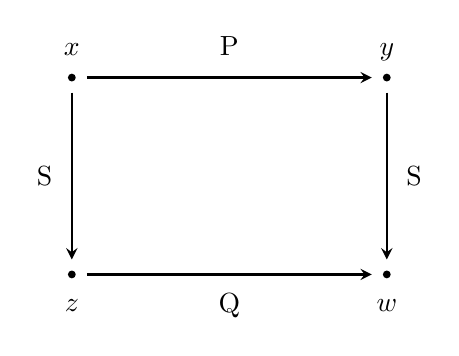
\begin{tikzpicture}
\usetikzlibrary{calc}
\pgfsetarrows{latex-latex};
\pgfsetarrowsend{latex};
\path node (z) at (0.5,-2.8) [shape=circle,inner sep=1pt,outer sep=4pt,fill,label=below:$z$] {}
      node (w) at (4.5,-2.8) [shape=circle,inner sep=1pt,outer sep=4pt,fill,label=below:$w$] {}
      node (x) at (0.5,-0.3) [shape=circle,inner sep=1pt,outer sep=4pt,fill,label={[label distance=-3pt]above:$x\vphantom{y}$}] {}
      node (y) at (4.5,-0.3) [shape=circle,inner sep=1pt,outer sep=4pt,fill,label={[label distance=-3pt]above:$y$}] {};
\draw [->,thick,>=stealth] (z) to (w);
\draw [->,thick,>=stealth] (x) to (z);
\draw [->,thick,>=stealth] (y) to (w);
\draw [->,thick,>=stealth] (x) to (y);
\node [label=below:Q] (q) at ($(z)!.5!(w)$) {};
\node [outer sep=4pt,label={[label distance=-3pt]above:P}] (p) at ($(x)!.5!(y)$) {};
\node [label=left:S] (p) at ($(x)!.5!(z)$) {};
\node [label=right:S] (p) at ($(w)!.5!(y)$) {};
\end{tikzpicture}
\end{wrapfigure}}
%
\newcommand{\figtwo}{\begin{wrapfigure}[11]{l}{1.55in}
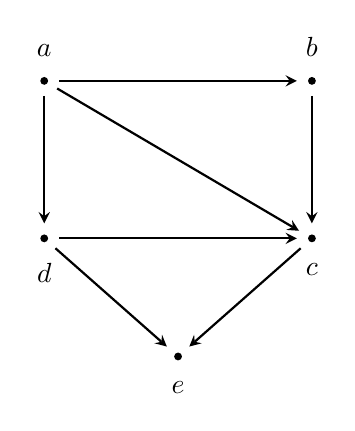
\begin{tikzpicture}
\path node (d) at (0.5,-2.3) [shape=circle,inner sep=1pt,outer sep=4pt,fill,label=below:$d$] {}
      node (c) at (3.9,-2.3) [shape=circle,inner sep=1pt,outer sep=4pt,fill,label=below:$c$] {} 
      node (a) at (0.5,-0.3) [shape=circle,inner sep=1pt,outer sep=4pt,fill,label=above:$a$] {}
      node (b) at (3.9,-0.3) [shape=circle,inner sep=1pt,outer sep=4pt,fill,label=above:$b$] {}
      node (e) at (2.2,-3.8) [shape=circle,inner sep=1pt,outer sep=4pt,fill,label=below:$e$] {};
\draw [->,thick,>=stealth] (a) to (b);
\draw [->,thick,>=stealth] (a) to (c);
\draw [->,thick,>=stealth] (a) to (d);
\draw [->,thick,>=stealth] (b) to (c);
\draw [->,thick,>=stealth] (c) to (e);
\draw [->,thick,>=stealth] (d) to (c);
\draw [->,thick,>=stealth] (d) to (e);
\end{tikzpicture}
\end{wrapfigure}}
%
% Inserts core document
% My own way of tracking the changes
\newcommand{\version}{$1.0$}
%
% % Marking changes from Allen and Unwin version
\newcommand{\change}[1]{\textcolor[rgb]{0,0.4,0}{#1}}
\newcommand{\kckaddition}[1]{\textcolor{red}{#1}}
%
% Some mathematical notation
\newcommand{\kktimes}{\mathbin{.}} % old multiplication dot
\newcommand{\kknicefrac}[2]{#1/#2} % in-paragraph fraction
\newcommand{\kkssb}{\mathrel{\vert}} % vertical Sheffer stroke
\newcommand{\kkssd}{\mathord{\raisebox{-.07em}{\rotatebox{10}{/}}}} % slanted Sheffer stroke

% For adding larger spaces after sentences ending in ellipses
\newcommand{\kksentencespace}{\spacefactor\sfcode`.{ }}

% makes Chapter numbers Roman
\renewcommand{\thechapter}{\Roman{chapter}}
%
% package for CC icons at end
\usepackage{ccicons}
%
\begin{document}
%
% Uses appropriate headers for full sized page versions
\lxonly{\pagestyle{myheadings}\markboth{\hfill\textit{Introduction to Mathematical Philosophy}\hfill}{}}
\ltronly{\pagestyle{myheadings}\markboth{\hfill\textit{Introduction to Mathematical Philosophy}\hfill}{}}
\afouronly{\pagestyle{myheadings}\markboth{\hfill\textit{Introduction to Mathematical Philosophy}\hfill}{}}
\aftonly{\pagestyle{myheadings}\markboth{\hfill\textit{Introduction to Mathematical Philosophy}\hfill}{}}
% begins font matter -- uses Roman numerals
\frontmatter
%
% Cover pages for the electronic versions
%
\ebkonly{%
    \begin{center}\thispagestyle{empty}
    \includegraphics[width=\textwidth]{CoverDesign.jpg}\clearpage
    \end{center}%
}
\iphoneonly{%
    \begin{center}
    \vspace*{4pt}\thispagestyle{empty}
    \includegraphics[width=\textwidth]{CoverDesign.jpg}\clearpage
    \end{center}
}
%
% The titlepage
%
    \thispagestyle{empty} 
    \begin{center}
    \vspace*{\titlepagetop}
    \Huge{\textbf{\ebkonly{\Large}\iphoneonly{\Large} Introduction to \iphoneonly{\\ \Large}Mathematical \iphoneonly{\\ \Large}Philosophy}}  \iphoneonly{\Large}\\
    \vspace*{\titlepageby}
    \Large{\ebkonly{\normalsize}\iphoneonly{\normalsize} by}\\
    \vspace*{\titlepageby} 
    \Large{\ebkonly{\normalsize}\iphoneonly{\normalsize} Bertrand Russell}\\
    \vspace*{\titlepagemiddle}
    \small{\iphoneonly{\scriptsize}\textit{Originally published by}}\\
    \normalfont{\iphoneonly{\scriptsize}George Allen \& Unwin, Ltd., London. May 1919. \allbutiphone{\\} Online Corrected Edition version \version\ (\today),\allbutiphone{\\} based on the ``second edition'' (second printing) of April 1920, incorporating additional corrections, \ebkonly{\\}\change{marked in green}.}\iphoneonly{\scriptsize}\\
    \end{center}
%
% Used to put content on right side for 2 sided version
\lxonly{\clearpage ~\setcounter{page}{0}}
% Do not put page numbers in ebook version
\ebkonly{\pagestyle{empty}}
%
% dustjacket text
\newlength{\dustjacketspace}
\setlength{\dustjacketspace}{0.1\textheight}
\ebkonly{\setlength{\dustjacketspace}{0.05\textheight}}
\iphoneonly{\setlength{\dustjacketspace}{0\textheight}}
\clearpage\vspace*{\dustjacketspace}
\noindent\kckaddition{[Russell's blurb from the original dustcover:]}\bigskip\\
\noindent This book is intended for those who have no previous acquaintance with the topics of which it treats, and no more knowledge of mathematics than can be acquired at a primary school or even at Eton. It sets forth in elementary form the logical definition of number, the analysis of the notion of order, the modern doctrine of the infinite, and the theory of descriptions and classes as symbolic fictions. The more controversial and uncertain aspects of the subject are subordinated to those which can by now be regarded as acquired scientific knowledge. These are explained without the use of symbols, but in such a way as to give readers a general understanding of the methods and purposes of mathematical logic, which, it is hoped, will be of interest not only to those who wish to proceed to a more serious study of the subject, but also to that wider circle who feel a desire to know the bearings of this important modern science.
%
% Sets spacing between ToC entriesl; different for different version
%
\iphoneonly{\setlength{\cftbeforechapskip}{.1em}}
\aftonly{\setlength{\cftbeforechapskip}{.0em}}
\ltronly{\setlength{\cftbeforechapskip}{.25em}}
\afouronly{\setlength{\cftbeforechapskip}{.3em}}
\lxonly{\setlength{\cftbeforechapskip}{.3em}}
\ebkonly{\setlength{\cftbeforechapskip}{.1em}}
%
% How far to right indent chapter numbers in ToC
\allbutiphone{\setlength{\cftchapnumwidth}{3.5em}}
\iphoneonly{\setlength{\cftchapnumwidth}{2.7em}}
%
% Sets dots to end of line in ToC
\renewcommand{\cftchapdotsep}{\cftdotsep}
%
% iPhoneOnly ToC settings; make unbold
\iphoneonly{\renewcommand{\cftchapfont}{\mdseries}%
\renewcommand{\cftchappagefont}{\mdseries}}
% Fills to right after ToC entry
\renewcommand{\cftchappresnum}{\hfill}
%
% Puts a period and space after a chapter number in ToC
\renewcommand{\cftchapaftersnum}{.\hspace*{0.5em}}

% Inserts table of contents
\iphoneonly{\tocloftpagestyle{empty}}
\clearpage\phantomsection%
\markboth{\normalsize\hfill\textit{Introduction to Mathematical Philosophy}\hfill}{\normalsize\hfill\textit{Contents}\hfill}
\addcontentsline{toc}{chapter}{Contents}\tableofcontents
\ebkonly{\thispagestyle{empty}}\iphoneonly{\thispagestyle{empty}}
%
\iphoneonly{\pagestyle{fancy}}
%
\clearpage\phantomsection\addcontentsline{toc}{chapter}{Preface}\chapter*{Preface}\iphoneonly{\vspace{-2cm}}\ebkonly{\thispagestyle{empty}}
\markboth{\normalsize\hfill\textit{Introduction to Mathematical Philosophy}\hfill}{\normalsize\hfill\textit{Preface}\hfill}
\kkparagraph{\noindent\kkpageindicatechapstart{v}{pagev}{\textsc{This}}  
 book is intended essentially as an ``Introduction,'' and
does not aim at giving an exhaustive discussion of the problems with
which it deals. It seemed desirable to set forth certain results,
hitherto only available to those who have mastered logical symbolism,
in a form offering the minimum of difficulty to the beginner. The
utmost endeavour has been made to avoid dogmatism on such questions as
are still open to serious doubt, and this endeavour has to some extent
dominated the choice of topics considered. The beginnings of
mathematical logic are less definitely known than its later portions,
but are of at least equal philosophical interest. Much of what is set
forth in the following chapters is not properly to be called
``philosophy,'' though the matters concerned were included in philosophy
so long as no satisfactory science of them existed. The nature of
infinity and continuity, for example, belonged in former days to
philosophy, but belongs now to mathematics. Mathematical \textit{philosophy}, in
the strict sense, cannot, perhaps, be held to include such definite
scientific results as have been obtained in this region; the philosophy
of mathematics will naturally be expected to deal with questions on the
frontier of knowledge, as to which comparative certainty is not yet
attained. But speculation on such questions is hardly likely to be
fruitful unless the more scientific parts of the principles of
mathematics are known. A book dealing with those parts may, therefore,
claim to be an \textit{introduction}
to mathematical philosophy, though it can hardly claim, except where it
steps outside its province, to be actually dealing with a part of
philosophy. It does deal, \kkpageindicate{vi}{pagevi} 
however, with a body of knowledge which, to
those who accept it, appears to invalidate much traditional philosophy,
and even a good deal of what is current in the present day. In this
way, as well as by its bearing on still unsolved problems, mathematical
logic is relevant to philosophy. For this reason, as well as on account
of the intrinsic importance of the subject, some purpose may be served
by a succinct account of the main results of mathematical logic in a
form requiring neither a knowledge of mathematics nor an aptitude for
mathematical symbolism. Here, however, as elsewhere, the method is more
important than
the results, from the point of view of further research; and the method
cannot well be explained within the framework of such a book as the
following. It is to be hoped that some readers may be sufficiently
interested to advance to a study of the method by which mathematical
logic can be made helpful in investigating the traditional problems of
philosophy. But that is a topic with which the following pages have not
attempted to deal.}
\\ \phantom{x} \hfill BERTRAND RUSSELL.
\clearpage\phantomsection\addcontentsline{toc}{chapter}{Editor's Note}%
\chapter*{Editor's Note}\iphoneonly{\vspace{-2cm}}\ebkonly{\thispagestyle{empty}}
\markboth{\normalsize\hfill\textit{Introduction to Mathematical Philosophy}\hfill}{\normalsize\hfill\textit{Editor's Note}\hfill}
\noindent\kkpageindicatechapstart{vii}{pagevii}{\kckaddition{[The}}\kckaddition{\ note below was written
by J.\ H.\ Muirhead, LL.D., editor of the Library of Philosophy series in which
\textit{Introduction to Mathematical Philosophy}
was originally published.]}

\phantom{x}

\noindent\textsc{Those} who, 
relying on the
distinction between Mathematical
Philosophy and the Philosophy of Mathematics, think that this book is
out of place in the present Library, may be referred to what the author
himself says on this head in the Preface. It is not necessary to agree
with what he there suggests as to the readjustment of the field of
philosophy by the transference from it to mathematics of such problems
as those of class, continuity, infinity, in order to perceive the
bearing of the definitions and discussions that follow on the work of
``traditional philosophy.'' If philosophers cannot consent to relegate
the criticism of these categories to any of the special sciences, it is
essential, at any rate, that they should know the precise meaning that
the science of mathematics, in which these concepts play so large a
part, assigns to them. If, on the other hand, there be mathematicians
to whom these definitions and discussions seem to be an elaboration and
complication of the simple, it may be well to remind them from the side
of philosophy that here, as elsewhere, apparent simplicity may conceal
a complexity which it is the business of somebody, whether philosopher
or mathematician, or, like the author of this volume, both in one, to
unravel.
\mainmatter%
\iphoneonly{\setcounter{origpage}{0}
\renewcommand{\theorigpage}{\arabic{origpage}}}
\chapter{The Series of Natural Numbers}\iphoneonly{\vspace{-1cm}}\ebkonly{\thispagestyle{empty}}
\markboth{\normalsize\hfill\textit{Introduction to Mathematical Philosophy}\hfill}{\normalsize\hfill\textit{Chap.\ \thechapter.\ \  The Series of Natural Numbers}\hfill}
\kkparagraph{\noindent\kkpageindicatechapstart{1}{page1}{\textsc{Mathematics}} is a 
study which, when we start from its most
familiar portions, may be pursued in either of two opposite directions.
The more familiar direction is constructive, towards gradually
increasing complexity: from integers to fractions, real numbers,
complex numbers; from addition and multiplication to differentiation
and integration, and on to higher mathematics. The other direction,
which is less familiar, proceeds, by analysing, to greater and greater
abstractness and logical simplicity; instead of asking what can be
defined and deduced from what is assumed to begin with, we ask instead
what more general ideas and principles can be found, in terms of which
what was our starting-point can be defined or deduced. It is the fact
of pursuing this opposite direction that characterises mathematical
philosophy as opposed to ordinary mathematics. But it
should be understood that the distinction is one, not
in the subject matter, but in the state of mind of the investigator.
Early Greek geometers, passing from the empirical rules of
Egyptian land-surveying to the general propositions by which those
rules were found to be justifiable, and thence to Euclid's axioms and
postulates, were engaged in mathematical philosophy, according to the
above definition; but when once the axioms and postulates had been
reached, their deductive employment, as we find it in Euclid, belonged
to mathematics in the \kkpageindicate{2}{page2} 
ordinary sense. The distinction between
mathematics and mathematical philosophy is one which depends upon the
interest inspiring the research, and upon the stage which the research
has reached; not upon the propositions with which the research is
concerned.}
\kkparagraph{We may state the same distinction in another way. The
most
obvious and easy things in mathematics are not those that come
logically at the beginning; they are things that, from the point of
view of logical deduction, come somewhere in the middle. Just as the
easiest bodies to see are those that are neither very near nor very
far, neither very small nor very great, so the easiest conceptions to
grasp are those that are neither very complex nor very simple (using
``simple'' in a \textit{logical}
sense). And as we need two sorts of instruments, the telescope
and the microscope, for the enlargement of our visual powers, so we
need two sorts of instruments for the enlargement of our logical
powers, one to take us forward to the higher mathematics, the other to
take us backward to the logical foundations of the things that we are
inclined to take for granted in mathematics. We shall find that by
analysing our ordinary mathematical notions we acquire fresh insight,
new powers, and the means of reaching whole new mathematical subjects
by adopting fresh lines of advance after our backward journey. It is
the purpose of this book to explain mathematical philosophy
simply and untechnically, without enlarging upon those portions which
are so doubtful or difficult that an elementary treatment is scarcely
possible. A full treatment will be found in \textit{Principia 
Mathematica};\footnote{Cambridge University Press, vol.\ i., 1910; vol.\ ii., \phantomsection\label{change:pmyear}\change{1912}; vol.\ iii., 
1913. By Whitehead and
Russell.} the treatment in the present volume is intended merely as an
introduction.}
\kkparagraph{To the average educated person of the present day, the
obvious
starting-point of mathematics \ebkonly{\linebreak[4]}would be the series of whole numbers,}\iphoneonly{

}\[1,\thickspace 2,\thickspace 3,\thickspace 4,\thickspace{\ldots}\thickspace\textup{etc.~}\kkpmarkonly\] 
\kkparagraph{\noindent \kkpnoteonly{3}{page3}Probably  
only a person with some mathematical knowledge
would
think of beginning with 0 instead of with 1, but we will presume this
degree of knowledge; we will take as our starting-point the series:}
\[0,\thickspace 1,\thickspace 2,\thickspace 3,\thickspace{\ldots}\thickspace n,\thickspace n+1,\thickspace{\ldots}\]
\kkparagraph{\noindent and it is this series that we shall
mean when we speak of the ``series of natural numbers.''}
\kkparagraph{It is only at a high stage of civilisation that we could
take
this series as our starting-point. It must have required many ages to
discover that a brace of pheasants and a couple of days were both
instances of the number 2: the degree of abstraction involved is far
from easy. And the discovery that 1 is a number must have been
difficult. As for 0, it is a very recent addition; the Greeks and
Romans had no such digit. If we had been embarking upon mathematical
philosophy in earlier days, we should have had to start with something
less abstract than the series of natural numbers, which we should reach
as a stage on our backward journey. When the logical foundations of
mathematics have grown more familiar, we shall be able to start
further back, at what is now a late stage in our analysis. But for the
moment the natural numbers seem to represent what is easiest and most
familiar in mathematics.}
\kkparagraph{But though familiar, they are not understood. Very few
people
are prepared with a definition of what is meant by ``number,'' or ``0,'' or
``1.'' It is not very difficult to see that, starting from 0, any other
of the natural numbers can be reached by repeated additions of 1, but
we shall have to define what we mean by ``adding 1,'' and what we mean by
``repeated.'' These questions are by no means easy. It was believed until
recently that some, at least, of these first notions of arithmetic must
be accepted as too simple and primitive to be defined. Since all terms
that are defined are defined by means of other terms,
it is clear that human knowledge must always be content to accept some
terms as intelligible without definition, in 
order \kkpageindicate{4}{page4} to have a
starting-point for its definitions. It is not clear that there must be
terms which are \textit{incapable}
of definition: it is possible that, however
far back we go in defining, we always \textit{might} go further
still. On the
other hand, it is also possible that, when analysis has been pushed far
enough, we can reach terms that really are simple, and therefore
logically incapable of the sort of definition that consists in
analysing. This is a question which it is not necessary for us to
decide; for our purposes it is sufficient to observe that, since human
powers are finite, the definitions known to us must always begin
somewhere, with terms undefined for the moment, though perhaps not
permanently.}
\kkparagraph{All traditional pure mathematics, including analytical
geometry, may be regarded as consisting wholly of propositions about
the natural
numbers. That is to say, the terms which occur can be defined by means
of the natural numbers, and the propositions can be deduced from the
properties of the natural numbers---with the addition, in
each case, of the ideas and propositions of pure logic.}
\kkparagraph{That all traditional pure mathematics can be derived
from the
natural numbers is a fairly recent discovery, though it had long been
suspected. Pythagoras, who believed that not only mathematics, but
everything else could be deduced from numbers, was the discoverer of
the most serious obstacle in the way of what is called the
``arithmetising'' of mathematics. It was Pythagoras who discovered the
existence of incommensurables,
and, in particular, the incommensurability of the side of a square and
the diagonal. If the length of the side is 1 inch, the number of inches
in the diagonal is the square root of 2, which appeared not to be a
number at all. The problem thus raised was solved only in our own day,
and was only solved \textit{completely}
by the help of the reduction of arithmetic to logic, which will be
explained in following chapters. For the present, we shall take for
granted the arithmetisation of mathematics, though this was a feat of
the very greatest importance.~\kkpmarkonly}
\kkparagraph{ Having\kkpnoteonly{5}{page5}
reduced all traditional pure mathematics to the theory
of the natural numbers, the next step in logical analysis was to reduce
this theory itself to the smallest set of premisses and undefined terms
from which it could be derived. This work was accomplished by Peano. He
showed that the entire theory of the natural numbers could be derived
from three primitive ideas and five primitive propositions in addition
to those of pure logic. These three ideas and five propositions thus
became, as it were, hostages for the whole of traditional pure
mathematics. If they could be defined and proved in terms of others, so
could all pure mathematics. Their logical ``weight,'' if one may use such
an expression, is equal to that of the whole series of sciences that
have been deduced from the theory of the natural numbers; the truth of
this whole series is assured if the truth of the five primitive
propositions is guaranteed, provided, of course, that there is nothing
erroneous in the purely logical apparatus which is also involved. The
work of analysing mathematics is extraordinarily facilitated by this
work of Peano's.}
\kkparagraph{The three primitive ideas in Peano's arithmetic are:}
\[0,\thickspace \text{number,}\thickspace \text{successor}.\]
\kkparagraph{\noindent By ``successor'' he means the next number in the natural
order.
That is to say, the successor of 0 is 1, the successor of 1 is 2, and
so on. By ``number'' he means, in this connection, the class of the
natural numbers.\footnote{\phantomsection\label{fn:example}We shall use ``number'' in
this sense in the present chapter.
Afterwards the word will be used in a more general sense.} He
is not assuming that we know all the members of this
class, but only that we know what we mean when we say that this or that
is a number, just as we know what we mean when we say ``Jones is a man,''
though we do not know all men individually.}
\kkparagraph{The five primitive propositions which Peano assumes are:}
\kkdisplay{(1) 0 is a number.
\item (2) The successor of any number is a number.
\item (3) No two numbers have the same successor. 
\kkpmarkonly 
\item (4) \kkpnoteonly{6}{page6}0 is not the successor of any number.
\item (5) Any property which belongs to 0, and also to the successor
of every number which has the property, belongs to all numbers.}
\kkparagraph{\noindent The last of these is the principle of mathematical
induction.
We shall have much to say concerning mathematical induction in
the sequel; for the present, we are concerned with it only as it occurs
in Peano's analysis of arithmetic.}
\kkparagraph{Let us consider briefly the kind of way in which the
theory of
the natural numbers results from these three ideas and five
propositions. To begin with, we define 1 as ``the successor of 0,'' 2 as
``the successor
of 1,'' and so on. We can obviously go on as long as we like with these
definitions, since, in virtue of (2), every number that we reach will
have a successor, and, in virtue of (3), this cannot be any of the
numbers already defined, because, if it were, two different numbers
would have the same successor; and in virtue of (4) none of the numbers
we reach in the series of successors can be 0. Thus the series of
successors gives us an endless series of continually new numbers. In
virtue of (5) all numbers come in this series, which begins with 0 and
travels on through successive successors: for (\textit{a}) 0 belongs to this
series, and (\textit{b}) if a number \textit{n}
belongs to it, so does its successor,
whence, by mathematical induction, every number belongs to the series.}
\kkparagraph{Suppose we wish to define the sum of two numbers. Taking
any
number $m$, we define $m+0$
as $m$, and $m+(n+1)$ as the
successor of $m+n$. In
virtue of (5) this gives a definition of the sum of \textit{m} and \textit{n}, whatever number \textit{n}
may be. Similarly we can define the product of any two
numbers. The reader can easily convince himself that any ordinary
elementary proposition of arithmetic can be proved by means of our five
premisses, and if he has any difficulty he can find the proof in Peano.}
\kkparagraph{It is time now to turn to the considerations which make
it
necessary to advance beyond the standpoint of Peano, who 
\kkpageindicate{7}{page7}  represents the
last perfection of the ``arithmetisation'' of mathematics, to that of
Frege, who first succeeded in ``logicising'' mathematics, \textit{i.e.}\ in
reducing to logic the arithmetical notions which his predecessors had
shown to be sufficient for mathematics. We shall not, in this chapter,
actually give Frege's
definition of number and of particular numbers, but we shall give some
of the reasons why Peano's treatment is less final than it appears to
be.}
\kkparagraph{In the first place, Peano's three primitive
ideas---namely, ``0,''
``number,'' and ``suc\-ces\-sor''---are capable of an infinite number of
different interpretations, all of which will satisfy the five primitive
propositions. We will give some examples.}
\kkparagraph{(1) Let ``0'' be taken to mean 100, and let ``number'' be
taken to
mean the numbers from 100 onward in the series of natural numbers. Then
all our primitive propositions are satisfied, even the fourth, for,
though 100 is the successor of 99, 99 is not a ``number'' in the sense
which we are now
giving to the word ``number.'' It is obvious that any number may be
substituted for 100 in this example.}
\kkparagraph{(2) Let ``0'' have its usual meaning, but let ``number''
mean what
we usually call ``even numbers,'' and let the ``successor'' of a number be
what results from adding two to it. Then ``1'' will stand for the number
two, ``2'' will stand for the number four, and so on; the series of
``numbers'' now will be}
\[0,\thickspace \textup{two,\thickspace four,\thickspace six,\thickspace eight}~{\ldots}\]
\kkparagraph{\noindent All Peano's five premisses are satisfied still.}
\kkparagraph{(3) Let ``0'' mean the number one, let ``number'' mean the
set}\iphoneonly{

}\[1,\thickspace \tfrac{1}{2},\thickspace \tfrac{1}{4},\thickspace \tfrac{1}{8},\thickspace \tfrac{1}{16},\thickspace\ldots\]
\kkparagraph{\noindent and let ``successor'' mean ``half.'' Then all
Peano's five axioms will be true of this set.}
\kkparagraph{It is clear that such examples might be multiplied
indefinitely. In fact, given any series}
\[\noindent x_0,\thickspace x_1,\thickspace x_2,\thickspace x_3,\thickspace{\ldots}\thickspace{x_n},\thickspace{\ldots}\thickspace\kkpmarkonly
\]
\kkparagraph{\noindent \kkpnoteonly{8}{page8}which is
endless, contains no repetitions,
has a beginning, and has no terms that cannot be reached from the
beginning in a finite number of steps, we have a set of terms verifying
Peano's axioms. This is easily seen, though the formal proof is
somewhat long. Let ``0'' mean $x_0$,
let ``number'' mean the whole set of terms,
and let the ``successor'' of $x_n$
mean $x_{n+1}$.
Then}
\kkparagraph{(1) ``0 is a number,'' \textit{i.e.}\ $x_0$
is a member of the set.}
\kkparagraph{(2) ``The successor of any number is a number,'' \textit{i.e.}\
taking any term $x_n$
in the set, $x_{n+1}$
is also in the set.}
\kkparagraph{(3) ``No two numbers have the same successor,'' \textit{i.e.}\
if $x_m$ and $x_n$
are
two different members of the set, $x_{m+1}$
and $x_{n+1}$ 
are different; this
results from the fact that (by hypothesis) there are no repetitions in
the set.}
\kkparagraph{(4) ``0 is not the successor of any number,'' \textit{i.e.}\ no term in
the set comes before $x_0$.}
\kkparagraph{(5) This becomes: Any property which belongs to $x_0$,
and belongs to $x_{n+1}$ 
provided it belongs to $x_n$,
belongs to all the $x$'s.}
\kkparagraph{This follows from the corresponding property for numbers.}
\kkparagraph{A series of the form}
\[%
x_0,\thickspace x_1,\thickspace x_2,\thickspace{\ldots}\thickspace{x_n},\thickspace{\ldots}
\]
\kkparagraph{\noindent in which there is a first term, a
successor to each term (so that there is no last term), no repetitions,
and every term can be reached from the start in a finite number of
steps, is called a \textit{progression}.
Progressions are of great importance in the
principles of mathematics. As we have just seen, every progression
verifies Peano's five axioms. It can be proved, conversely, that every
series which verifies Peano's five axioms is a progression. Hence these
five axioms may be used to define the class of progressions:
``progressions'' are ``those series which verify these five axioms.'' Any
progression may be taken as the basis of pure mathematics: we may give
the name ``0'' to its first term, the name ``number'' to the whole set of
its terms, and the name ``successor'' to the next in the progression. The
progression need not be composed of numbers: it may 
be \kkpageindicate{9}{page9}  composed of points in space,
or moments of time, or any other terms of
which there is an infinite supply. Each different progression will give
rise to a different interpretation of all the propositions of
traditional pure mathematics; all these possible interpretations will
be equally true.}
\kkparagraph{In Peano's system there is nothing to enable us to
distinguish between these different interpretations of his primitive
ideas. It is assumed that we know what is meant by ``0,'' and that we
shall not suppose that this symbol means 100 or Cleopatra's Needle or
any of the other things that it might mean.}
\kkparagraph{This point, that ``0'' and ``number'' and ``successor'' cannot
be
defined by means of Peano's five axioms, but must be independently
understood, is important. We want our numbers not merely to verify
mathematical formul{\ae}, but to apply in the right way to common objects.
We want to have ten fingers and two eyes and one nose. A system in
which ``1'' meant 100, and ``2'' meant 101, and so on, might be all right
for pure mathematics, but would not suit daily life. We want ``0'' and
``number'' and ``successor'' to have meanings which will give us the right
allowance of fingers and eyes and noses. We have already some knowledge
(though not sufficiently
articulate or analytic) of what we mean by ``1'' and ``2'' and so on, and
our use of numbers in arithmetic must conform to this knowledge. We
cannot secure that this shall be the case by Peano's method; all that
we can do, if we adopt his method, is to say ``we know what we mean by
`0' and `number' and `successor,' though we cannot explain what we mean
in
terms of other simpler concepts.'' It is quite legitimate to say this
when we must, and at \textit{some} point we all must; but it is the object of
mathematical philosophy to put off saying it as long as possible. By
the logical theory of arithmetic we are able to put it off for a very
long time.}
\kkparagraph{It might be suggested that, instead of setting up ``0''
and
``number'' and ``successor'' as terms of which we know the meaning although
we cannot define them, we might let them \kkpageindicate{10}{page10}  stand for \textit{any}
three terms
that verify Peano's five axioms. They will then no longer be terms
which have a meaning that is definite though undefined: they will be
``variables,'' terms concerning which we make certain hypotheses, namely,
those stated in the five axioms, but which are otherwise undetermined.
If we adopt this plan, our theorems will not be proved concerning an
ascertained set of terms called ``the natural numbers,'' but concerning
all sets of terms having certain properties. Such a procedure is not
fallacious; indeed for certain purposes it represents a valuable
generalisation. But from two points of view it fails to give an
adequate basis for arithmetic. In the first place, it does not enable
us to know whether there are any sets of terms verifying Peano's
axioms; it does not even give the faintest suggestion of any way of
discovering whether there are such sets. In the second place, as
already observed, we want our
numbers to be such as can be used for counting common objects, and this
requires that our numbers should have a \textit{definite} meaning,
not merely that they should
have certain formal properties. This definite meaning is defined by the
logical theory of arithmetic.}
\chapter{Definition of Number}\iphoneonly{\vspace{-1cm}}\ebkonly{\thispagestyle{empty}}
\markboth{\normalsize\hfill\textit{Introduction to Mathematical Philosophy}\hfill}{\normalsize\hfill\textit{Chap.\ \thechapter.\ \  Definition of Number}\hfill}
\kkparagraph{\noindent\kkpageindicatechapstart{11}{page11}{\textsc{The}} question ``What is a
number?''\ is
one which has been often
asked, but
has only been correctly answered in our own time. The answer was given
by Frege in 1884, in his \textit{Grundlagen
der Arithmetik}.\footnote{The same answer is given
more fully and with more
development in his
\textit{Grundgesetze der
Arithmetik}, vol.\ i.,\ 1893.} Although
this book
is quite short, not difficult, and of the very highest importance, it
attracted almost no attention, and the definition of number which it
contains remained
practically unknown until it was rediscovered by the present author in
1901.}
\kkparagraph{In seeking a definition of number, the first thing to be
clear
about is
what we may call the grammar of our inquiry. Many philosophers, when
attempting to define number, are really setting to work to define
plurality, which is quite a different thing. \textit{Number} is what is
characteristic of numbers, as \textit{man}
is what is characteristic of men. A
plurality is not an instance of number, but of some particular number.
A trio of men, for example, is an instance of the number 3, and the
number 3 is an instance of number; but the trio is not an instance of
number. This point may seem elementary and scarcely worth mentioning;
yet it has proved too subtle for the philosophers, with few exceptions.}
\kkparagraph{A particular number is not identical with any collection
of
terms
having that number: the number 3 is not identical with \kkpageindicate{12}{page12}  the trio
consisting of Brown, Jones, and Robinson. The number 3 is something
which all trios have in common, and which distinguishes them from
other collections. A number is something that characterises certain
collections, namely, those that have that number.}\afouronly{\enlargethispage{\baselineskip}}
\kkparagraph{Instead of speaking of a ``collection,'' we shall as a
rule
speak of a
``class,'' or sometimes a ``set.'' Other words used in mathematics for the
same thing are ``aggregate'' and ``manifold.'' We shall have much to say
later on about classes. For the present, we will say as little as
possible. But there are some remarks that must be made immediately.}
\kkparagraph{A class or collection may be defined in two ways that at
first
sight
seem quite distinct. We may enumerate its members, as when we say, ``The
collection I mean is Brown, Jones, and Robinson.'' Or we may mention a
defining property, as when we speak of ``mankind'' or ``the inhabitants of
London.'' The definition which enumerates is called a definition by
``extension,'' and the one which mentions a defining property is called a
definition by ``intension.'' Of these two kinds of definition, the one by
intension is logically more fundamental. This is shown by two
considerations: (1) that the extensional definition can always be
reduced to an intensional one; (2) that the intensional one often
cannot even theoretically be reduced to the extensional one. Each of
these points needs a word of explanation.}
\kkparagraph{(1) Brown, Jones, and Robinson all of them possess a
certain
property
which is possessed by nothing else in the whole universe, namely, the
property of being either Brown or Jones or Robinson. This 
property can be used to give a definition by
intension
of
the
class consisting of Brown and Jones and Robinson. Consider such a
formula as ``\textit{x}
is Brown or \textit{x}
is Jones or \textit{x}
is Robinson.'' This formula will be true for just three \textit{x}'s, namely, Brown
and Jones
and Robinson. In this respect it resembles a cubic equation with its
three roots. It may be taken as assigning a property common to the
members of the class consisting of these three \kkpageindicate{13}{page13}  men, and peculiar to
them. A similar treatment can obviously be applied to any other class
given in extension.}%\aftonly{\enlargethispage{\baselineskip}}
\kkparagraph{(2) It is obvious that in practice we can often know a
great
deal about
a class without being able to enumerate its members. No one man could
actually enumerate all men, or even all the
inhabitants of London, yet a great deal is known about each of these
classes. This is enough to show that definition by extension is not
\textit{necessary}
to knowledge about a class. But when we come to consider
infinite classes, we find that enumeration is not even theoretically
possible for beings who only live for a finite time. We cannot
enumerate all the natural numbers: they are 0, 1,
2,
3, \textit{and
so on}. At some point we must content ourselves with ``and
so on.'' We
cannot enumerate all fractions or all irrational numbers, or all of any
other infinite collection. Thus our knowledge in regard to all such
collections can only be derived from a definition by intension.}
\kkparagraph{These remarks are relevant, when we are seeking the
definition
of
number, in three different ways. In the first place, numbers themselves
form an infinite collection, and cannot therefore be defined by
enumeration. In the second place, the collections having a given number
of terms themselves presumably form an infinite collection: it is to be
presumed, for example, that there are an infinite collection of trios
in the world, for if this were not the case the total number of things
in the world would be finite, which, though possible, seems unlikely.
In the third place, we wish to define ``number'' in such a way that
infinite numbers may be possible; thus we must be able to speak of the
number of terms in an infinite collection, and such a collection must
be defined by intension, \textit{i.e.}\ by a property common to all its members
and peculiar to them.}
\kkparagraph{For many purposes, a class and a defining characteristic
of
it
are
practically interchangeable. The vital difference between the two
consists in the fact that there is only one class having a given set of
members, whereas there are always many different characteristics by
which a given class may be defined. Men \kkpageindicate{14}{page14}  may be defined as featherless
bipeds, or as rational animals, or (more correctly) by the traits by
which Swift delineates the Yahoos. \hypertarget{c2n2}{It} is this fact that a defining
characteristic is never unique which makes classes useful; otherwise we
could be content with the properties common and peculiar to their
members.\footnote{As will be explained
later, classes may be regarded as
logical
fictions, manufactured out of defining characteristics. But for the
present it will simplify our exposition to treat classes as if they
were real.} Any one of
these properties can be used in place of the
class whenever uniqueness is not important.}
\kkparagraph{Returning now to the definition of number, it is clear
that
number is a
way of bringing together certain collections, name\-ly, those that have a
given number of terms. We can suppose all couples in one bundle, all
trios in another, and so on. In this way we obtain various bundles of
collections, each bundle consisting of all the collections that have a
certain number of terms. Each bundle is a class whose members are
collections, \textit{i.e.}\ classes; thus each is a class of classes. The bundle
consisting of all couples, for example, is a class of classes: each
couple is a class with two members, and the whole bundle of couples is
a class with an infinite number of members, each of which is a class of
two members.}
\kkparagraph{How shall we decide wheth\-er two collections are to
belong to
the same
bundle? The answer that suggests itself is: ``Find out how many members
each has, and put them in the same bundle if they have the same number
of members.'' But this presupposes that we have defined numbers, and
that we know how to discover how many terms a collection has. We are so
used to the operation of counting that such a presupposition might
easily pass unnoticed. In fact, however, counting, though familiar, is
logically a very complex operation; moreover it is only available, as
a means of discovering how many terms a collection has, when the
collection is finite. Our definition of number must not assume in
advance that all numbers are finite; and we cannot in any case, without
a vicious circle, \kkpageindicate{15}{page15} 
use counting to define numbers, because numbers are
used in counting. We need, therefore, some other method of deciding
when two collections have the same number of terms.}
\kkparagraph{In actual fact, it is simpler logically to find out
whether
two
collections have the same number of terms than it is to define what
that number is. An illustration will make this clear. If there were no
polygamy or polyandry anywhere in the
world,
it is
clear that the number of husbands living at any moment would be exactly
the same as the number of wives. We do not need a census to assure us
of this, nor do we need to know what is the actual number of husbands
and of wives. We know the number must be the same in both collections,
because each husband has one wife and each wife has one husband. The
relation of husband and wife is what is called ``one-one.''}
\kkparagraph{A relation is said to be ``one-one'' when, if \textit{x} has the
relation
in
question to \textit{y},
no other term $x^\prime$
has the same relation to \textit{y},
and \textit{x} does
not have the same relation to any term $y^\prime$ other 
than \textit{y}. When only the
first of these two conditions is fulfilled, the relation is called
``one-many''; when only the second is fulfilled, it is called ``many-one.''
It should be observed that the number 1 is not used in these
definitions.}
\kkparagraph{In Christian countries, the relation of husband to wife
is
one-one; in
Mahometan countries it is one-many; in Tibet it is many-one. The
relation of father to son is one-many; that of son to father is
many-one, but that of eldest son to father is one-one. If \textit{n} is any
number, the relation of \textit{n}
to $n+1$ is
one-one; so is the relation of \textit{n}
to $2n$ or to
$3n$. When we
are considering only positive numbers, the
relation of \textit{n}
to $n^2$ is one-one; but when negative numbers are admitted,
it becomes two-one, since \textit{n}
and $-n$ have
the same square. These instances
should suffice to make clear the notions of one-one, one-many, and
many-one relations, which play a great part in the principles of
mathematics, not only in relation to the definition of numbers, but in
many other connections.}
\kkparagraph{Two classes are said to be ``similar'' when there is a
one-one \kkpageindicate{16}{page16}  relation
which correlates the terms of the one class each with one term of the
other class, in the same manner in which the relation of marriage
correlates husbands with wives. A few preliminary definitions will help
us to state this definition more precisely. The class of those terms
that have a given relation to something or other is called the \textit{domain}
of that relation: thus fathers are the domain of the relation of father
to child, husbands are the domain of the relation of husband to wife,
wives are the domain of the relation of wife to husband, and husbands
and wives together are the domain of the relation of marriage. The
relation of wife to husband is called the \textit{converse} of the
relation of
husband to wife. Similarly \textit{less}
is the converse of \textit{greater},
\textit{later}
is
the converse of \textit{earlier},
and so on. Generally, the converse of a given
relation is that relation which holds between \textit{y} and \textit{x} whenever the
given relation holds between \textit{x}
and \textit{y}. The
\textit{converse domain}
of a relation
is the domain of its converse: thus the class of wives is the converse
domain of the relation of husband to wife. We may now state our
definition of similarity as follows:---}
\kkparagraph{\textit{One class is said to
be
``similar'' to another when there is a
one-one
relation of which the one class is the domain, while the other is the
converse domain.}}
\kkparagraph{It is easy to prove (1) that every class is similar to
itself, (2) that if a class \ensuremath{\alpha} is similar to 
a class \ensuremath{\beta}, then \ensuremath{\beta} is
similar to \ensuremath{\alpha},
(3) that if \ensuremath{\alpha} is similar 
to \ensuremath{\beta} and \ensuremath{\beta} to \ensuremath{\gamma}, 
then \ensuremath{\alpha} is similar to \ensuremath{\gamma}. A
relation is said to be \textit{reflexive}
when it possesses the first of these
properties, \textit{symmetrical}
when it possesses the second, and \textit{transitive}
when it possesses the third. It is obvious that a relation which is
symmetrical and transitive must be reflexive throughout its domain.
Relations which possess these properties are an important kind, and it
is worth while to note that similarity is one of this kind of relations.}
\kkparagraph{It is obvious to common sense that two finite classes
have
the
same
number of terms if they are similar, but not otherwise. The act of
counting consists in establishing a one-one
correlation \kkpageindicate{17}{page17}  be\-tween
the set of objects counted and the natural numbers (excluding
0) that are used up in the process. Accordingly common sense concludes
that there are as many objects in the set to be counted as there are
numbers up to the last number used in the counting. And we also know
that, so long as we confine ourselves to finite numbers, there are just
\textit{n}
numbers
from 1 up to \textit{n}.
Hence it follows that the last number used in
counting a collection is the number of terms in the collection,
provided the collection is finite. But this result, besides being only
applicable to finite collections, depends upon and assumes the fact
that two classes which are similar have the same number of terms; for
what we do when we count (say) 10 objects is to show that the set of
these objects is similar to the set of numbers 1 to 10. The notion of
similarity is logically presupposed in the operation of counting, and
is logically simpler though less familiar. In counting, it is necessary
to take the objects counted in a certain order, as first, second,
third, etc., but order is not of the essence of number: it is an
irrelevant addition, an unnecessary complication from the logical
point of view. The notion of similarity does not demand an order: for
example, we saw that the number of husbands is the same as the number
of wives, without having to establish an order of precedence among
them. The notion of similarity also does not require that the classes
which are similar should be finite. Take, for example, the natural
numbers (excluding 0) on the one hand, and the fractions which have 1
for their numerator on the other hand: it is obvious that we can
correlate 2 with \phantomsection\label{fracchange17}$\kknicefrac{1}{2}$, 3 with $\kknicefrac{1}{3}$, and so on, thus proving
that the two classes are similar.\\
\indent We may thus use the notion of ``similarity'' to decide
when two
collections are to belong to the same bundle, in the sense in which we
were asking this question earlier in this chapter. We want 
to make one bundle containing the class that has
no
members:
this will be for the number 0. Then we want a bundle of all the classes
that have one member: this will be for the number 1. Then, for the
number 2, we want a bundle consisting \kkpageindicate{18}{page18}  of all couples; then one of all
trios; and so on. Given any collection, we can define the bundle it is
to belong to as being the class of all those collections that are
``similar'' to it. It is very easy to see that if (for example) a
collection has three members, the class of all those collections that
are similar to it will be the class of trios. And whatever number of
terms a collection may have, those collections that are ``similar'' to it
will have the same number of terms. We may take this as a \textit{definition} of
``having the same number of terms.'' It is obvious that it gives results
conformable to usage so long as we confine ourselves to finite
collections.}
\kkparagraph{So far we have not suggested anything in the slightest
degree
paradoxical. But when we come to the actual definition of numbers we
cannot avoid what must at first sight seem a paradox, though this
impression will soon wear off. We naturally think that the class of
couples (for example) is something different from the number 2. But
there is no doubt about the class of couples: it is indubitable and not
difficult to define, whereas the number 2, in any other sense, is a
metaphysical entity about which we can never feel sure that it exists
or that we have tracked it down. It is therefore more prudent to
content ourselves with the class of couples, which we are sure of, than
to hunt for a problematical number 2 which must always remain elusive.
Accordingly we set up the following definition:---}
\kkparagraph{\textit{The number of a class
is
the class of all those classes that
are
similar to it.}}
\kkparagraph{Thus the number of a couple will be the class of all
couples.
In fact, the class of all couples will \textit{be} the number 2,
according to
our definition. At the expense of a little oddity, this definition
secures definiteness and indubitableness; and it is not difficult to
prove that numbers so defined have all the properties that we expect
numbers to have.}
\kkparagraph{We may now go on to define numbers in general as any one
of
the bundles
into which similarity collects classes. A number will be a set of
classes such as that any two are similar to each \kkpageindicate{19}{page19} other, and none
outside the set are similar to any inside the set. In 
other words, a number (in general) is any collection
which
is the
number of one of its members; or, more simply still:}
\kkparagraph{\textit{A number is anything
which
is the number of some class.}}
\kkparagraph{Such a definition has a verbal appearance of being
circular,
but in
fact it is not. We define ``the number of a given class'' without using
the notion of number in general; therefore we may define number in
general in terms of ``the number of a given class'' without committing
any logical error.}
\kkparagraph{Definitions of this sort are in fact very common. The
class
of
fathers,
for example, would have to be defined by first defining what it is to
be the father of somebody; then the class of fathers will be all those
who are somebody's father. Similarly if we want to define square
numbers (say), we must first define what we mean by saying that one
number is the square of another, and then define square numbers as
those that are the squares of other numbers. This kind of procedure is
very common, and it is important to realise that it is legitimate and
even often necessary.}
\kkparagraph{We have now given a definition of numbers which will
serve
for
finite
collections. It remains to be seen how it will serve for infinite
collections. But first we must decide what we mean by ``finite'' and
\ebkonly{\linebreak[4]\clearpage\noindent\negmedspace}``infinite,'' which cannot be \iphoneonly{\linebreak[4]\clearpage\noindent}done within the limits of the present
chapter.}
\chapter{Finitude and Mathematical Induction}\iphoneonly{\vspace{-1cm}}\ebkonly{\thispagestyle{empty}}
\markboth{\normalsize\hfill\textit{Introduction to Mathematical Philosophy}\hfill}{\normalsize\hfill\textit{Chap.\ \thechapter.\ \  Finitude and Mathematical Induction}\hfill}
\kkparagraph{\noindent\kkpageindicatechapstart{20}{page20}{\textsc{The}} 
series of natural numbers, as we saw in Chapter I.,
can
all be
defined if we know what we mean by the three terms ``0,'' ``number,'' and
``successor.'' But we may go a step farther: we can define all the
natural numbers if we know what we mean by ``0'' and ``successor.'' It will
help us to understand the difference between finite and infinite to see
how this can be done, and why the method by which it is done cannot be
extended beyond the finite. We will not yet consider how ``0'' and
``successor'' are to be defined: we will for the moment assume that we
know what these terms mean, and show how thence all other natural
numbers can be obtained.}\lxonly{\enlargethispage{\baselineskip}}
\kkparagraph{It is easy to see that we can reach any assigned number,
say
30,000. We
first define ``1'' as ``the successor of 0,'' then we define ``2'' as ``the
successor of 1,'' and so on. In the case of an assigned number, such as
30,000, the proof that we can reach it by proceeding step by step in
this fashion may be made, if we have the patience, by actual
experiment: we can go on until we actually arrive at 30,000. But
although the method of experiment is available for each particular
natural number, it is not available for proving the general proposition
that \textit{all} such numbers can be reached in this way, \textit{i.e.}\ by proceeding
from 0 step by step from each number to its successor. Is there any
other way by which this can be proved?}\afouronly{\enlargethispage{\baselineskip}}
\kkparagraph{Let us consider the question the other way round. What
are
the
numbers
that can be reached, given the terms ``0'' and \kkpageindicate{21}{page21}  ``successor''? Is there any
way
by which we can define the whole class of such numbers? We reach 1, as
the successor of 0; 2, as the successor of 1; 3, as the successor of 2;
and so on. It is this ``and so on'' that we wish to replace by something
less vague and indefinite. We might be tempted to say that ``and so on''
means that the process of proceeding to the successor may be repeated
\textit{any finite number}
of times; but the problem upon which we are engaged
is the problem of defining ``finite number,'' and therefore we must not
use this notion in our definition. Our definition must not assume that
we know what a finite number is.}\lxonly{\enlargethispage{\baselineskip}}
\kkparagraph{The key to our problem lies in \textit{mathematical induction}.
It
will
be
remembered that, in Chapter I., this was the fifth of the five
primitive propositions which we laid down about the natural numbers. It
stated that any property which belongs to 0, and to the successor of
any number which has the property, belongs to all the natural numbers.
This was then presented as a principle, but we shall now adopt it as a
definition. It is not difficult to see that the terms obeying it are
the same as the numbers that can be reached from 0 by successive steps
from next to next, but as the point is important we will set forth the
matter in some detail.}
\kkparagraph{We shall do well to begin with some definitions, which
will
be
useful
in other connections also.}
\kkparagraph{A property is said to be ``hereditary'' in the
na\-tural-number
series if,
whenever it belongs to a number \textit{n},
it also belongs to $n+1$,
the
successor of \textit{n}.
Similarly a class is said to be ``hereditary'' if,
whenever $n$ is a member of the class, so is $n+1$. It is easy to \textit{see},
though we are not yet supposed to know, that to say a property is
hereditary is equivalent to saying that it belongs to all the natural
numbers not less than some one of them, \textit{e.g.}\ it must belong
to all that
are not less than 100, or all that are \phantomsection\label{change:notless}\change{not} less than 1000, or it may be
that it belongs to all that are not less than 0, \textit{i.e.}\ to all without
exception.}
\kkparagraph{A property is said to be ``inductive'' when it is a
hereditary \kkpageindicate{22}{page22}  property
which belongs to 0. Similarly a class is ``inductive'' when it is a
hereditary class of which 0 is a member.}
\kkparagraph{Given a hereditary class of which 0 is a member, it
follows
that 1 is a
member of it, because a hereditary class contains the successors of its
members, and 1 is the successor of 0. Similarly, given a hereditary
class of which 1 is a member, it follows that 2 is a member of it; and
so on. Thus we can prove by a step-by-step procedure that any assigned
natural number, say 30,000, is a member of every inductive class.}
\kkparagraph{We will define the ``posterity'' of a given natural number
with
respect
to the relation
``immediate predecessor'' (which is the converse of
``successor'') as all those terms that belong to every hereditary class
to which the given number belongs. It is again easy to \textit{see} that the
posterity of a natural number consists of itself and all greater
natural numbers; but this also we do not yet officially know.}
\kkparagraph{By the above definitions, the posterity of 0 will
consist of
those
terms which belong to every inductive class.}
\kkparagraph{It is now not difficult to make it obvious that the
posterity
of 0 is
the same set as those terms that can be reached from 0 by successive
steps from next to next. For, in the first place, 0 belongs to both
these sets (in the sense in which we have defined our terms); in the
second place, if \textit{n}
belongs to both sets, so does $n+1$.
It is to be
observed that we are dealing here with the kind of matter that does not
admit of precise proof, namely, the comparison of a relatively vague
idea with a relatively precise one. The notion of ``those terms that can
be reached from 0 by successive steps from next to next'' is
vague,
though it \textit{seems}
as if it conveyed a definite meaning; on the other
hand, ``the posterity of 0'' is precise and explicit just where the other
idea is hazy. It may be taken as giving what we \textit{meant} to mean when
we
spoke of the terms that can be reached from 0 by successive steps.}
\kkparagraph{We now lay down the following definition:---}
\kkparagraph{\textit{The
``natural
numbers'' are
the posterity of} 0 \textit{with respect to the} \kkpageindicate{23}{page23}  \textit{relation ``immediate predecessor''} (which is the converse of
``successor'').}
\kkparagraph{We have thus arrived at a definition of one of Peano's
three
primitive ideas in terms of the other two. As a result of this
definition, two of
his primitive propositions---namely, the one asserting that 0 is a number
and the one asserting mathematical induction---become unnecessary, since
they result from the definition. The one asserting that the successor
of a natural number is a natural number is only needed in the weakened
form ``every natural number has a successor.''}
\kkparagraph{We can, of course, easily define ``0'' and ``successor'' by
means
of the definition of number in
general which we arrived at in Chapter II.\ The number 0 is the number
of terms in a class which has no members, \textit{i.e.}\ in the class
which is
called the ``null-class.'' By the general definition of number, the
number
of terms in the null-class is the set of all classes similar to the
null-class, \textit{i.e.}\ (as is easily proved) the set consisting of the
null-class all alone, \textit{i.e.}\ the class whose only member is the
null-class. (This is not identical with the null-class: it has one
member, namely, the null-class, whereas the null-class itself has no
members. A class which has one member is never identical with that one
member, as we shall explain when we come to the theory of classes.)
Thus we have the following purely logical definition:--- }


0 \textit{is the class
whose only member is the null-class.}

\kkparagraph{It remains to define ``successor.'' Given any number \textit{n}, let \ensuremath{\alpha} be a class
which has \textit{n}
members, and let \textit{x}
be a term which is not a member of \ensuremath{\alpha}.
Then the class consisting of \ensuremath{\alpha} with \textit{x} added on will
have $n+1$
members.
Thus we have the following definition:---}
\kkparagraph{\textit{The
successor
of the number of terms in the class \ensuremath{\alpha} is the
number of
terms in the class consisting of} \ensuremath{\alpha} \textit{together with} x, \textit{where} x \textit{is any term
not belonging to the class.}}
\kkparagraph{Certain niceties are required to make this definition
perfect,
but they
need not concern us.\footnote{See \textit{Principia Mathematica},
vol.\ ii.\ $*\thinspace$110.} It will be remembered
that we \kkpageindicate{24}{page24}  have already
given
(in Chapter II.) a logical definition of the number of terms in a
class, namely, we defined it as the set of all classes that are similar
to the given class.}\afouronly{\enlargethispage{\baselineskip}}
\kkparagraph{We have thus reduced Pea\-no's three primitive ideas to
ideas
of
logic:
we have given definitions of them which make them definite, no longer
capable of an infinity of different meanings, as they were when they
were only determinate to the extent of obeying Peano's five axioms. We
have removed them from the fundamental apparatus of terms that must be
merely apprehended, and have thus increased the deductive articulation
of mathematics.}
\kkparagraph{As regards the five primitive propositions, we have
already
succeeded
in making two of them demonstrable by our definition of ``natural
number.'' How stands it with the remaining three? It is very easy to
prove that 0 is not the successor of any
number, and
that the successor of any number is a number. But there is a difficulty
about the remaining primitive proposition, namely, ``no two numbers have
the same successor.'' The difficulty does not arise unless the total
number of individuals in the universe is finite; for given two numbers
\textit{m} and
\textit{n},
neither of which
is the total number of individuals in the
universe, it is easy to prove that we cannot have $m+1=n+1$ unless we
have $m=n$. But let us
suppose that the total number of individuals in the
universe were (say) 10; then there would be no class of 11 individuals,
and the number 11 would be the null-class. So would the number 12.
Thus we should have $11=12$; therefore the successor of 10 would be the
same as the successor of 11, although 10 would not be the same as 11.
Thus we should have two different numbers with the same successor. This
failure of the third axiom cannot arise, however, if the number of
individuals in the world is not finite. We shall return to this topic
at a
later stage.\footnote{See Chapter XIII.}}
\kkparagraph{Assuming that the number of individuals in the universe
is
not
finite,
we have now succeeded not only in defining Peano's \kkpageindicate{25}{page25}  three primitive
ideas, but in seeing how to prove his five primitive propositions, by
means of primitive ideas and propositions belonging to logic. It
follows that all pure mathematics, in so far as it is deducible from
the theory of the natural numbers, is only a prolongation of logic. The
extension of this result to those modern branches of mathematics which
are not deducible from the theory of the natural numbers offers no
difficulty of principle, as we have shown elsewhere.\footnote{For geometry, in so far
as it is not purely analytical,
see
\textit{Principles of
Mathematics},
part vi.; for rational dynamics, \textit{ibid}.,
part
vii.}}
\kkparagraph{The process of mathematical induction, by means of which
we
defined the
natural numbers, is capable of generalisation. We defined the natural
numbers as the ``posterity'' of 0 with
respect to
the relation of a number to its immediate successor. If we call this
relation N, any number \textit{m}
will have this
relation to $m+1$.
A property is ``hereditary with respect to N,'' or simply
``N-hereditary,'' if, whenever the property belongs to a number \textit{m}, it
also belongs to $m+1$,
\textit{i.e.}\ to the
number to which \textit{m}
has the relation N.
And a number \textit{n}
will be said to belong to the ``posterity'' of \textit{m} with
respect to the relation N if \textit{n}
has every N-hereditary property
belonging to \textit{m}.
These definitions can all be applied to any other
relation just as well as to N. \hypertarget{fregenote1}{Thus} if R is any relation whatever, we
can lay down the following definitions:\footnote{These definitions, and
the generalised theory of
induction,
are due
to Frege, and were published so long ago as 1879 in his
\textit{Begriffsschrift}. In spite of the great value of this work, I was, I
believe, the first person who ever read it---more than twenty years after
its publication.}---}
\kkparagraph{A property is called ``R-hereditary'' when, if it belongs
to a
term \textit{x},
and \textit{x} has
the relation R to \textit{y},
then it belongs to \textit{y}.}
\kkparagraph{A class is R-hereditary when its defining property is
R-heredi\-tary.}
\kkparagraph{A term \textit{x}
is said to be an ``R-ancestor'' of the term \textit{y} if \textit{y}
has
every
R-hereditary property that \textit{x}
has, provided \textit{x}
is a term which has the
relation R to something or to which something has the relation R. (This
is only to exclude trivial cases.)}
\kkpmarkonly 
\kkparagraph{The \kkpnoteonly{26}{page26}``R-posterity'' of \textit{x}
is all the terms of which \textit{x}
is an
R-ances\-tor.}
\kkparagraph{We have framed the above definitions so that if a term
is
the
ancestor
of anything it is its own ancestor and belongs to its own posterity.
This is merely for convenience.}
\kkparagraph{It will be observed that if we take for R the relation
``parent,''
``ancestor'' and ``posterity'' will have the usual meanings, except that a
person will be included among his own ancestors and posterity. It is,
of course, obvious at once that ``ancestor'' must be capable of
definition in terms of ``parent,'' but until Frege developed his
generalised theory of induction, no one could have defined ``ancestor''
precisely in terms of ``parent.'' A brief consideration of this point
will serve to show the importance of the theory. A person confronted
for the first time with the problem of defining ``ancestor'' in terms of
``parent'' would naturally say that A is an ancestor of Z if, between A
and Z, there are a certain number of people, B, C, {\ldots}, of whom B is
a child of A, each is a parent of the next, until the last, who is a
parent of Z. But this definition is not adequate unless we add that the
number of intermediate terms is to be finite. Take, for example, such a
series as the following:---}
\[-1,\thickspace -\tfrac{1}{2},\thickspace -\tfrac{1}{4},\thickspace -\tfrac{1}{8},\thickspace \ldots\thickspace \tfrac{1}{8},\thickspace \tfrac{1}{4},\thickspace \tfrac{1}{2},\thickspace 1.\]
\kkparagraph{\noindent Here we have first a series of negative fractions with
no
end, and then a series of positive fractions with no beginning. Shall we say that, in
this series, \phantomsection\label{fracchange26}$-\kknicefrac{1}{8}$ is an ancestor of $\kknicefrac{1}{8}$? It will be so according to the
beginner's definition suggested above, but it will not be so according
to any definition which will give the kind of idea that we wish to
define. For this purpose, it is essential that the number of
intermediaries should be finite. But, as we saw, ``finite'' is to be
defined by means of
mathematical
induction, and it is simpler to define the ancestral relation generally
at once than to define it first only for the case of the relation of \textit{n}
to $n+1$,
and then extend it to other cases. Here, as constantly
elsewhere, generality from the first, though it may \kkpageindicate{27}{page27}  require more
thought at the start, will be
found in the long run to economise thought and increase logical power.}
\kkparagraph{The use of mathematical induction in demonstrations was,
in
the past,
something of a mystery. There seemed no reasonable doubt that it was a
valid method of proof, but no one quite knew why it was valid. Some
believed it to be really a case of induction, in the sense in which
that word is used in logic. Poincar\'e\footnote{\textit{Science and
Method}, chap.\ iv.} considered it to be a
principle of the utmost
importance, by
means of which an infinite number of syllogisms could be condensed into
one argument. We now know that all such views are mistaken, and that
mathematical induction is a definition, not a principle. There are some
numbers to which it can be applied, and there are others (as we shall
see in Chapter VIII.) to which it cannot be applied. We \textit{define} the
``natural numbers'' as those to which proofs by mathematical induction
can be applied, \textit{i.e.}\ as those that possess all inductive properties. It
follows that such proofs can be applied to the natural numbers, not in
virtue of any mysterious intuition or axiom or principle, but as a
purely verbal proposition. If ``quadrupeds'' are defined as animals
having four legs, it will follow that animals that have four legs are
quadrupeds; and the case of numbers that obey mathematical induction is
exactly similar.}
\kkparagraph{We shall use the phrase ``inductive numbers'' to mean the
same
set as we
have hitherto spoken of as the ``natural numbers.'' The phrase ``inductive
numbers'' is preferable as affording a
reminder
that the definition of this set of numbers is obtained from
mathematical induction.}
\kkparagraph{Mathematical induction affords, more than anything else,
the
essential
characteristic by which the finite is distinguished from the infinite.
The principle of mathematical induction might be stated popularly in
some such form as ``what can be inferred from next to next can be
inferred from first to last.'' This is true when the number of
intermediate steps between
first and
last is finite, not otherwise. Anyone who has ever \kkpageindicate{28}{page28}  watched a goods
train beginning to move will have noticed how the impulse is
communicated with a jerk from each truck to the next, until at last
even the hindmost truck is in motion. When the train is very long, it
is a very long time before
the
last
truck moves. If the train were infinitely long, there would be an
infinite succession of jerks, and the time would never come when the
whole train would be in motion. Nevertheless, if there were a series of
trucks no longer than the series of inductive numbers (which, as we
shall see, is an instance of the smallest of infinites), every truck
would begin to move sooner or later if the engine persevered, though
there would always be other trucks further back which had not yet begun
to move. This image will help to elucidate the argument from next to
next, and its connection with finitude. When we come to infinite
numbers, where arguments from mathematical induction will be no longer
valid, the properties of such numbers will help to make clear, by
contrast, the almost unconscious use that is made of mathematical
induction where finite numbers are concerned.}
\chapter{The Definition of Order}\iphoneonly{\vspace{-1cm}}\ebkonly{\thispagestyle{empty}}
\markboth{\normalsize\hfill\textit{Introduction to Mathematical Philosophy}\hfill}{\normalsize\hfill\textit{Chap.\ \thechapter.\ \ The Definition of Order}\hfill}
\kkparagraph{\noindent\kkpageindicatechapstart{29}{page29}{\textsc{We}} have now carried our
analysis of the series of natural numbers to the point where we
have
obtained logical definitions of the members of this series, of the whole class
of its members, and of the relation of a number to its immediate
successor. We must now consider the \textit{serial} character of
the natural
numbers in the order 0, 1, 2, 3, {\ldots} We ordinarily think of the
numbers as in this \textit{order},
and it is an essential part of the work of
analysing our data to seek a definition of ``order'' or ``series'' in
logical terms.}
\kkparagraph{The notion of order is one which has enormous importance
in
mathematics. Not only the integers, but also rational fractions and
all real numbers have an order of magnitude, and this is essential to
most of their mathematical properties. The order of points on a line is
essential to geometry; so is the slightly more complicated order of
lines through a point in a plane, or of planes through a line.
Dimensions, in geometry, are a development of order. The conception of
a \textit{limit},
which underlies all higher mathematics, is a serial
conception. There are parts of mathematics which do not depend upon the
notion of order, but they are very few in comparison with the parts in
which this notion is involved.}
\kkparagraph{In seeking a definition of order, the first thing to
realise
is that no
set of terms has just \textit{one}
order to the exclusion of others. A set of terms has all the orders of
which it is capable.
Sometimes
one order is so much more familiar and natural to our \kkpageindicate{30}{page30}  thoughts that we
are inclined to regard it as \textit{the}
order of that set of terms; but this
is a mistake. The natural numbers---or the ``inductive'' numbers, as we
shall also call them---occur to us most readily in order of magnitude;
but they are capable of an infinite number of other arrangements. We
might, for example, consider first all the odd numbers and then all the
even numbers; or first 1, then all the even numbers, then all the odd
multiples of 3, then all the multiples of 5 but not of 2 or 3, then all
the multiples of 7 but not of 2 or 3 or 5, and so on through the whole
series of primes. When we say that we ``arrange'' the numbers in these
various orders, that is an inaccurate expression: what we really do is
to turn our attention to certain relations between the natural numbers,
which themselves generate such-and-such an arrangement. We can no more
``arrange'' the natural numbers than we can the starry heavens; but just
as we may notice among the fixed stars either their order of brightness
or their distribution in the sky, so there are various relations among
numbers which may be observed, and which give rise to various different
orders among numbers, all equally legitimate. And what is true of
numbers is equally true of points on a line or of the moments of time:
one order is more familiar, but others are equally valid. We might, for
example, take first, on a line, all the points that have integral
co-ordinates, then all those that have non-integral rational
co-ordinates, then all those that have algebraic non-rational
co-ordinates, and so on, through any set of complications we please.
The resulting order will be one which the points of the line certainly
have, whether we choose to notice it or not; the only thing that is
arbitrary about the various orders of a set of terms is our attention,
for the terms themselves have always all the orders of which they are
capable.\lxonly{\enlargethispage{\baselineskip}}\aftonly{\enlargethispage{\baselineskip}}

One important result of this consideration is that we
must
not
look for
the definition of order in the nature of the set of terms to be
ordered, since one set of terms has many orders. The order lies, not in
the \textit{class}
of terms, but in a relation
among \kkpageindicate{31}{page31}  the
members of the class, in respect of which some appear as earlier and
some as later. The fact that a class may have many orders is due to the
fact that there can be many relations holding among the members of one
single class. What properties must a relation have in order to give
rise to an order?}
\kkparagraph{The essential characteristics of a relation which is to
give
rise to
order may be discovered by considering that in respect of such a
relation we must be able to say, of any two terms in the class which is
to be ordered, that one ``precedes'' and the other ``follows.'' Now, in
order that we may be able to use these words in the way in which we
should naturally understand them, we require that the ordering relation
should have three properties:---}\afouronly{\enlargethispage{\baselineskip}}
\kkparagraph{(1) If \textit{x}
precedes \textit{y},
\textit{y}
must not
also precede \textit{x}.
This is an
obvious
characteristic of the kind of relations that lead to series. If \textit{x} is less than \textit{y}, \textit{y} is not also less
than \textit{x}. If
\textit{x} is
earlier in time
than \textit{y}, \textit{y} is not also
earlier than \textit{x}.
If \textit{x} is to
the left of \textit{y},
\textit{y} is
not to the left of \textit{x}.
On the other hand, relations which do not give
rise to series often do not have this property. If \textit{x} is a brother or
sister of \textit{y},
\textit{y} is
a
brother or sister of \textit{x}.
If \textit{x} is of
the same height
as \textit{y}, \textit{y} is of the same
height as \textit{x}.
If \textit{x} is of
a different height from
\textit{y}, \textit{y} is of a different
height from \textit{x}.
In all these cases, when the
relation holds between \textit{x}
and \textit{y}, it
also holds between \textit{y}
and \textit{x}. But
with
serial relations such a thing cannot happen. A relation having this
first property is called \textit{asymmetrical}.}\lxonly{\enlargethispage{\baselineskip}}\aftonly{\enlargethispage{\baselineskip}}
\kkparagraph{(2) If \textit{x}
precedes \textit{y}
and \textit{y}
precedes \textit{z},
\textit{x}
must
precede \textit{z}.
This
may be
illustrated by the same instances as before: \textit{less}, \textit{earlier}, \textit{left of}.
But as instances of relations which do \textit{not} have this
property only two
of our previous three instances will serve. If \textit{x} is brother or
sister of \textit{y},
and \textit{y} of \textit{z}, \textit{x} may not be
brother or
sister of \textit{z},
since \textit{x}
and \textit{z} may
be the same person. The same applies to
difference of height, but not to sameness of height, which has our
second property but not our first. The relation ``father,'' on the other
hand, has our first property but not \kkpageindicate{32}{page32}  our second. A relation having our
second property is called \textit{transitive}.}
\kkparagraph{(3) Given any two terms of the class which is to be
ordered,
there must
be one which precedes and the other which follows. For example, of any
two integers, or fractions, or real
numbers, one is
smaller and the other greater; but of any two complex numbers this is
not true. Of any two moments in time, one must be earlier than the
other; but of events, which may be simultaneous, this cannot be said.
Of two points on a line, one must be to the left of the other. A
relation having this third property is called \textit{connected}.}
\kkparagraph{When a relation possesses these three properties, it is
of
the
sort to
give rise to an order among the terms between which it holds; and
wherever an order exists, some relation having these three properties
can be found generating it.}
\kkparagraph{\hypertarget{peircenote}{Before} illustrating this thesis, we will introduce a few
definitions.}
\kkparagraph{(1) A relation is said to be an 
aliorelative,\footnote{This term is due to C.\ S.\ Peirce.}
or to \textit{be
contained in}
or \textit{imply diversity},
if no term has this relation to itself. Thus, for example, ``greater,''
``different in size,''
``brother,''
``husband,'' ``father'' are aliorelatives; but ``equal,'' ``born of the same
parents,'' ``dear friend'' are not.}
\kkparagraph{(2) The \textit{square}
of a relation is that relation which holds
between two
terms \textit{x}
and \textit{z} when
there is an intermediate term \textit{y}
such that the given
relation holds between \textit{x}
and \textit{y} and
between \textit{y}
and \textit{z}.
Thus ``paternal
grandfather'' is the square of ``father,'' ``greater by 2'' is the square of
``greater by 1,'' and so on.}
\kkparagraph{(3) The \textit{domain}
of a relation consists of all those terms
that
have the
relation to something or other, and the \textit{converse domain}
consists of all
those terms to which something or other has the relation. These words
have been already defined, but are recalled here for the sake of the
following definition:---}
\kkparagraph{(4) The \textit{field}
of a relation consists of its domain and
converse domain
together.}
\kkpmarkonly
\kkparagraph{(5) \kkpnoteonly{33}{page33}One relation is said to \textit{contain} or \textit{be implied by}
another
if it
holds whenever the other holds.}
\kkparagraph{It will be seen that an \textit{asymmetrical}
relation is the same
thing as a
relation whose square is an aliorelative. It often happens that a
relation is an aliorelative without being asymmetrical, though an
asymmetrical relation is always an aliorelative. For example, ``spouse''
is an aliorelative, but is symmetrical, since if \textit{x} is the spouse of \textit{y},
\textit{y} is
the
spouse of \textit{x}.
But among \textit{transitive}
relations, all aliorelatives
are asymmetrical as well as \textit{vice
versa}.}
\kkparagraph{From the definitions it will be seen that a \textit{transitive}
relation is one
which is implied by its square, or, as we also say, ``contains'' its
square. Thus ``ancestor'' is transitive, because an ancestor's ancestor
is an ancestor; but ``father'' is not transitive, because a father's
father is not a father. A transitive aliorelative is one which contains
its square and is contained in diversity; or, what comes to the same
thing, one whose square implies both it and diversity---because, when a
relation is transitive, asymmetry is equivalent to being an
aliorelative.}
\kkparagraph{A relation is \textit{connected}
when, given any two different terms
of
its
field, the relation holds between the first and the second or between
the second and the first (not excluding the possibility that both may
happen, though both cannot happen if the relation is asymmetrical).}
\kkparagraph{It will be seen that the relation ``ancestor,'' for
example,
is
an
aliorelative and transitive, but not connected; it is because it is not
connected that it does not suffice to arrange the human race in a
series.}
\kkparagraph{The relation ``less than or equal to,'' among numbers, is
transitive and
connected, but not asymmetrical or an aliorelative.}
\kkparagraph{The relation ``greater or less'' among numbers is an
aliorelative and is
connected, but is not transitive, for if \textit{x} is greater or
less than \textit{y},
and \textit{y} is
greater or less than \textit{z},
it may happen that \textit{x}
and \textit{z} are
the
same number.}
\kkparagraph{Thus the three properties of being (1) an aliorelative,
(2)
\kkpageindicate{34}{page34}  tran\-si\-tive,
and (3) connected, are mutually independent, since a relation may have
any two without having the third.}
\kkparagraph{We now lay down the following definition:---}
\kkparagraph{A relation is \textit{serial}
when it is an aliorelative, transitive,
and
connected; or, what is equivalent, when it is asymmetrical, transitive,
and connected.}
\kkparagraph{A \textit{series}
is the same thing as a serial relation.}
\kkparagraph{It might have been thought that a series should be the
\textit{field}
of a
serial relation, not the serial relation itself. But this would be an
error. For example,}
\begin{equation*}\iphoneonly{\begin{gathered}}1,\medspace 2,\medspace 3;\thickspace 1,\medspace 3,\medspace 2;\thickspace 2,\medspace 3,\medspace 1;\thickspace 2,\medspace 1,\medspace 3;\iphoneonly{\\}\thickspace 3,\medspace 1,\medspace 2;\thickspace 3,\medspace
2,\medspace
1\iphoneonly{\end{gathered}}\end{equation*}
\kkparagraph{\noindent are six different series which all have the same field.
If the
field
\textit{were}
the
series, there could only be one series with a given field.
What distinguishes the above six series is simply the different
ordering relations in the six cases. Given the ordering relation, the
field and the order are both determinate. Thus the ordering relation
may be taken to \textit{be}
the series, but the field cannot be so taken.}
\kkparagraph{Given any serial relation, say P, we shall say that, in
respect of this
relation, \textit{x}
``precedes'' \textit{y}
if \textit{x} has
the relation P to \textit{y},
which we shall
write ``\textit{x}P\textit{y}'' for short. The
three characteristics which P must have in
order to be serial are:}
\kkdisplay{(1) We must never have
\textit{x}P\textit{x}, \textit{i.e.}\ no term must
precede itself.
\item (2) $\textup{P}^2$ must imply P, \textit{i.e.}\ if \textit{x} precedes \textit{y} and \textit{y} precedes $z$,
\textit{x}
must
precede $z$.
\item (3) If \textit{x}
and \textit{y} are
two different terms in the field of P, we
shall have
\textit{x}P\textit{y} or \textit{y}P\textit{x}, \textit{i.e.}\ one of the
two must precede the other.}
\kkparagraph{\noindent The reader can easily convince himself that, where these
three
properties are found in an ordering relation, the characteristics we
expect of series will also be found, and \textit{vice versa}. We are
therefore
justified in taking the above as a definition of order \kkpageindicate{35}{page35}  or series. And
it will be observed that the definition is
effected in purely logical terms.}\aftonly{\enlargethispage{\baselineskip}}
\kkparagraph{Although a transitive asymmetrical connected relation
always
exists
wherever there is a series, it is not always the relation which would
most naturally be regarded as generating the series. The natural-number
series may serve as an illustration. The
relation we
assumed in considering the natural numbers was the relation of
immediate succession, \textit{i.e.}\ the relation between consecutive integers.
This relation is asymmetrical, but not transitive or connected. We can,
however, derive from it, by the method of mathematical induction, the
``ancestral'' relation which we considered in the preceding chapter. This
relation will be the same as ``less than or equal to'' among inductive
integers. For purposes of generating the series of natural numbers, we
want the relation ``less than,'' excluding ``equal to.'' This is the
relation of \textit{m }to
\textit{n}
when \textit{m} is
an ancestor of
\textit{n} but
not
identical with \textit{n},
or
(what comes to the same thing) when the successor of \textit{m} is an ancestor
of \textit{n} in
the sense in which a number is its own ancestor. That is to
say, we shall lay down the following definition:---}
\kkparagraph{An inductive number \textit{m}
is said to be \textit{less than}
another number
\textit{n}
when \textit{n}
possesses every hereditary property possessed by the successor of \textit{m}.}
\kkparagraph{It is easy to see, and not difficult to prove, that the
relation ``less
than,'' so defined, is asymmetrical, transitive, and connected, and has
the inductive numbers for its field. Thus by means of this relation the
inductive numbers acquire an order in the sense in which we defined the
term ``order,'' and this order is the so-called ``natural'' order, or order
of magnitude.}\aftonly{\enlargethispage{\baselineskip}}
\kkparagraph{The generation of series by means of relations more or
less
resembling
that of \textit{n}
to $n+1$ is
very common. The series of the Kings of England,
for example, is generated by relations of each to his successor. This
is probably the easiest way, where it is applicable, of conceiving the
generation of a series. In this method we pass on from each term to the
next, as long as there \kkpageindicate{36}{page36} 
is a next, or back to the one before, as long as
there is one before. This method always requires the generalised form
of mathematical
induction in order to enable us to define ``earlier'' and ``later'' in a
series so generated. On the analogy of ``proper fractions,'' let us give
the name ``proper posterity of $x$ with respect to R'' to the class of
those terms that belong to the R-posterity of some term to which $x$ has
the relation R, in the sense which we gave before to ``posterity,'' which
includes a term in its own posterity. Reverting to the fundamental
definitions, we find that the ``proper posterity'' may be defined as
follows:---}
\kkparagraph{The ``proper posterity'' of $x$ with respect to R consists
of
all
terms
that possess every R-here\-ditary property possessed by every term to
which $x$ has the relation R.}
\kkparagraph{It is to be observed that this definition has to be so
framed
as to be
applicable not only when there is only one term to which $x$ has the
relation R, but also in cases (as \textit{e.g.}\ that of father and child) where
there may be many terms to which \textit{x}
has the relation R. We define
further:}
\kkparagraph{A term \textit{x}
is a ``proper ancestor'' of \textit{y}
with respect to R if \textit{y}
belongs to
the proper posterity of \textit{x}
with respect to R.}
\kkparagraph{We shall speak for short of ``R-posterity'' and
``R-an\-ces\-tors''
\aftonly{\linebreak[4]}when these
terms seem more convenient.}\afouronly{\enlargethispage{\baselineskip}}
\kkparagraph{Reverting now to the generation of series by the
relation R
between
consecutive terms, we see that, if this method is to be possible, the
relation ``proper R-ancestor'' must be an aliorelative, transitive, and
connected. Under what circumstances will this occur? It will always be
transitive: no matter what sort of relation R may be, ``R-ancestor'' and
``proper R-ancestor'' are always both transitive. But it is only under
certain circumstances that it will be an aliorelative or connected.
Consider, for example, the relation to one's left-hand neighbour at a
round dinner-table at which there are twelve people. If we call this
relation R, the proper R-posterity of a person consists of all who can
be reached by going round the table from right to left. This includes
everybody at the table, including the person himself, 
since \kkpageindicate{37}{page37}  twelve
steps bring us back to our
starting-point. Thus in such a case, though the relation ``proper
R-ancestor'' is connected, and though R itself is an aliorelative, we do
not get a series because ``proper R-ancestor'' is not an aliorelative. It
is for this reason that we cannot say that one person comes before
another with respect to the relation ``right of'' or to its ancestral
derivative.}
\kkparagraph{The above was an instance in which the ancestral
relation
was
connected
but not contained in diversity. An instance where it is contained in
diversity but not connected is derived from the ordinary sense of the
word ``ancestor.'' If \textit{x}
is a proper ancestor of \textit{y},
\textit{x} and
\textit{y}
cannot be the
same person; but it is not true that of any two persons one must be an
ancestor of the other.}
\kkparagraph{The question of the circumstances under which series can
be
generated
by ancestral relations derived from relations of consecutiveness is
often important. Some of the most important cases are the following:
Let R be a many-one relation, and let us confine our attention to the
posterity of some term \textit{x}.
When so confined, the relation ``proper
R-ancestor'' must be connected; therefore all that remains to ensure its
being serial is that it shall be contained in diversity. This is a
generalisation of the instance of the dinner-table. Another
generalisation consists in taking R to be a one-one relation, and
including the ancestry of \textit{x}
as well as the posterity. Here again, the
one condition required to secure the generation of a series is that the
relation ``proper R-ancestor'' shall be contained in diversity.}
\kkparagraph{The generation of order by means of relations of
consecutiveness,
though important in its own sphere, is less general than the method
which uses a transitive relation to define the order. It often happens
in a series that there are an infinite number of intermediate terms
between any two that may be selected, however near together these may
be. Take, for instance, fractions in order of magnitude. Between any
two fractions there are others---for example, the arithmetic mean of the
two. Consequently there is no such thing as a pair of consecutive
fractions. If we de\-pen\-ded~\kkpageindicate{38}{page38} u\-pon consecutiveness for defining order, we
should not be able to define the order of magnitude among fractions.
But in fact the relations of greater and less among fractions do not
demand generation from relations of consecutiveness, and the relations
of greater and less among fractions have the three characteristics
which we need for defining serial relations. In all such cases the
order must be defined by means of a \textit{transitive}
relation, since only
such a relation is able to leap over an infinite number of intermediate
terms. The method of consecutiveness, like that of counting for
discovering the number of a collection, is appropriate to the finite;
it may even be extended to certain infinite series, namely, those in
which, though the total number of terms is infinite, the number of
terms between any two is always finite; but it must not be regarded as
general. Not only so, but care must be taken to eradicate from the
imagination all habits of thought resulting from supposing it general.
If this is not done, series in which there are no consecutive terms
will remain difficult and puzzling. And such series are of vital
importance for the understanding of continuity, space, time, and motion.}\afouronly{\enlargethispage{\baselineskip}}
\kkparagraph{There are many ways in which series may be generated,
but
all
depend
upon the finding or construction of an asymmetrical transitive
connected relation. Some of these ways have considerable importance.
We may take as illustrative the generation of series by means of a
three-term relation which we may call ``between.'' This method is very
useful in geometry, and may serve as an introduction to relations
having more than two terms; it is best introduced in connection with
elementary geometry.}
\kkparagraph{Given any three points on a straight line in ordinary
space,
there must
be one of them which is \textit{between} the other two. This will not be the
case with the points on a circle or any other closed curve,
because,
given any three points on a circle, we can travel from any one to any
other without passing through the third. In 
fact, the notion ``between'' is characteristic of open
series---or
series in the strict sense---as opposed to what may be called \kkpageindicate{39}{page39}  ``cyclic''
series, where, as with people at the dinner-table, a sufficient journey
brings us back to our starting-point. This notion of ``between'' may be
chosen as the fundamental notion of ordinary geometry; but for the
present we will only consider its application to a single straight line
and to the ordering of the points on a straight line.\footnote{Cf.\ \textit{Rivista di Matematica},
iv.\ pp.\ 55ff.; \textit{Principles
of
Mathematics},
p.\ 394 ({\S}375).} Taking any two
points \textit{a},
\textit{b},
the line
(\textit{ab})
consists of three parts (besides \textit{a}
and \textit{b}
themselves):}
\kkdisplay{(1) Points between \textit{a} and \textit{b}. 
\item (2) Points \textit{x}
such that \textit{a}
is between \textit{x}
and \textit{b}.
\item (3) Points \textit{y}
such that \textit{b}
is between \textit{y}
and \textit{a}.}
\kkparagraph{\noindent Thus the line (\textit{ab})
can be defined in terms of the relation
``between.''}
\kkparagraph{In order that this relation ``between'' may arrange the
points
of the
line in an order from left to right, we need certain assumptions,
namely, the following:---}

(1) If anything is
between \textit{a}
and \textit{b}, \textit{a} and \textit{b} are not
identical.

(2) Anything between \textit{a}
and \textit{b} is
also between \textit{b}
and \textit{a}.

(3) Anything between \textit{a}
and \textit{b} is
not identical with \textit{a} (nor,
consequently, with \textit{b},
in virtue of (2)).

(4) If \textit{x}
is between \textit{a}
and \textit{b},
anything between \textit{a}
and \textit{x} is
also
between \textit{a}
and \textit{b}.

(5) If \textit{x}
is between \textit{a}
and \textit{b}, and
\textit{b} is
between \textit{x}
and \textit{y},
then
\textit{b}
is
between $a$ and $y$.
 
(6) If \textit{x}
and \textit{y} are
between \textit{a}
and \textit{b},
then either \textit{x}
and \textit{y} are
identical,
or \textit{x} is
between \textit{a}
and \textit{y}, or \textit{x} is between \textit{y} and \textit{b}.

(7) If \textit{b}
is between \textit{a}
and \textit{x} and
also between \textit{a}
and \textit{y},
then
either \textit{x}
and \textit{y} are
identical, or \textit{x}
is between \textit{b} and \textit{y},
or \textit{y} is
between \textit{b}
and \textit{x}.

\kkparagraph{These seven properties are obviously verified in the
case of
points on
a straight line in ordinary space. Any three-term relation which
verifies them gives rise to series, as may be seen from the following
definitions. For the sake of definiteness, let us 
\allbutiphone{as\-sume \kkpageindicate{40}{page40} that}%
\iphoneonly{as\-sume~\kkpageindicate{40}{page40}~that} \textit{a} is to
the left of \textit{b}.
Then the points of the line (\textit{ab})
are (1) those between
which and \textit{b},
\textit{a}
lies---these we will call to the left of \textit{a}; (2) \textit{a}
itself;
(3) those between \textit{a}
and \textit{b}; (4)
\textit{b}
itself;
(5) those between which and \textit{a}
lies \textit{b}---these we will call to the right of \textit{b}.
We may now define
generally that of two points \textit{x}, \textit{y},
on the line (\textit{ab}), we shall say that
\textit{x} is ``to the left of'' \textit{y} in
any of the following cases:---}
\kkdisplay{(1) When \textit{x}
and \textit{y} are
both to the left of \textit{a},
and \textit{y} is
between
\textit{x}
and \textit{a}; 
\item (2) When \textit{x}
is to the left of \textit{a},
and \textit{y} is \textit{a} or \textit{b} or between \textit{a}
and \textit{b} or
to the right of \textit{b};
\item (3) When \textit{x}
is \textit{a}, and \textit{y} is between \textit{a} and \textit{b} or is \textit{b} or is to
the right of
\textit{b};
\item (4) When \textit{x}
and \textit{y} are both between \textit{a} and \textit{b},
and \textit{y} is between \textit{x}
and \textit{b}; 
\item (5) When \textit{x}
is between \textit{a}
and \textit{b}, and \textit{y}
is \textit{b} or to
the
right of \textit{b}; 
\item (6) When \textit{x}
is \textit{b} and \textit{y}
is to the right of \textit{b}; 
\item (7) When \textit{x}
and \textit{y} are
both to the right of \textit{b}
and \textit{x} is
between
\textit{b}
and \textit{y}.}
\kkparagraph{It will be found that, from the seven properties which
we
have
assigned
to the relation ``between,'' it can be deduced that the relation ``to the
left of,'' as above defined, is a \textit{serial}
relation as we defined that
term. It is important to notice that nothing in the definitions or the
argument depends upon our meaning by ``between'' the actual relation of
that name which occurs in empirical space: any three-term relation
having the above seven purely formal properties will serve the purpose
of the argument equally well.}
\kkparagraph{Cyclic order, such as that of the points on a circle,
cannot
be
generated by means of three-term relations of ``between.'' We need a
relation of four terms, which may be called ``separation of couples.''
The point may be illustrated by considering a journey round the world.
One may go from England to New Zealand by way of Suez or by way of San
Francisco; we cannot \kkpageindicate{41}{page41} say definitely that
either of these two places is ``between'' England and New Zealand. But if
a man chooses that route to go round the world, whichever way round he
goes, his times in England and New Zealand are separated from each
other by his times in Suez and San Francisco, and conversely.
Generalising, if we take any four points on a circle, we can separate
them into two couples, say \textit{a}
and \textit{b} and \textit{x} and \textit{y}, such that, in
order to
get from \textit{a}
to \textit{b} one
must pass through either \textit{x}
or \textit{y}, and
in order to
get from \textit{x}
to \textit{y} one
must pass through either \textit{a}
or \textit{b}.
Under these
circumstances we say that the couple (\textit{a}, \textit{b}) are ``separated''
by the
couple (\textit{x}, \textit{y}). Out of this
relation a cyclic order can be generated,
in a way resembling that in which we generated an open order from
``between,'' but somewhat more complicated.\footnote{Cf.\ \textit{Principles of Mathematics},
p.\ 205 ({\S}194), and
references
there
given.}}
\kkparagraph{The purpose of the latter half of this chapter has been
to
suggest the
subject which one may call ``generation of serial relations.'' When such
relations have been defined, the generation of
them
from
other relations possessing only some of the properties required for
series becomes very important, especially in the philosophy of geometry
and physics. But we cannot, within the limits of the present volume, do
more than make the reader aware that such a subject exists.}
\chapter{Kinds of Relations}\iphoneonly{\vspace{-1cm}}\ebkonly{\thispagestyle{empty}}
\markboth{\normalsize\hfill\textit{Introduction to Mathematical Philosophy}\hfill}{\normalsize\hfill\textit{Chap.\ \thechapter.\ \  Kinds of Relations}\hfill}
\kkparagraph{\noindent\kkpageindicatechapstart{42}{page42}{\textsc{A great}} part of the philosophy of mathematics is
concerned
with
\textit{relations},
and many different kinds of relations have different kinds
of uses. It often happens that a property which belongs to \textit{all}
relations is only important as regards relations of certain sorts; in
these cases the reader will not see the bearing of the proposition
asserting such a property unless he has in mind the sorts of relations
for which it is useful. For reasons of this description, as well as
from the intrinsic interest of the subject, it is well to have in our
minds a rough list of the more mathematically serviceable varieties of
relations.}
\kkparagraph{We dealt in the preceding chapter with a su\-premely
important
class,
namely, \textit{serial}
relations. Each of the three properties which we
combined in defining series---namely, \textit{asymmetry}, \textit{transitiveness}, and
\textit{connexity}---has
its own importance. We will begin by saying something on
each of these three.}
\kkparagraph{\textit{Asymmetry},
\textit{i.e.}\ the
property of being incompatible with the
converse,
is a characteristic of the very greatest interest and importance. In
order to develop its functions, we will consider various examples. The
relation \textit{husband}
is asymmetrical, and so is the relation \textit{wife}; \textit{i.e.}\ if
\textit{a} is
husband of \textit{b},
\textit{b}
cannot be
husband of \textit{a},
and similarly in the case
of \textit{wife}.
On the other hand, the relation ``spouse'' is symmetrical: if \textit{a}
is spouse of \textit{b},
then \textit{b} is
spouse of \textit{a}.
Suppose now we are given the
relation \textit{spouse},
and we wish to derive the relation \textit{husband}.
\textit{Husband}
is
the same as \textit{male spouse}
or \textit{spouse of a female};
thus the relation
\textit{husband }can
\kkpageindicate{43}{page43}  be derived from
\textit{spouse}
either by limiting the domain to
males or by limiting the converse \phantomsection\label{change:conversedomain}\change{domain} to females. We see from this instance
that, when a symmetrical relation is given, it is sometimes possible,
without the help of any further relation, to separate it into two
asymmetrical relations. But the cases where this is possible are rare
and exceptional: they are cases where there are two mutually exclusive
classes, say \ensuremath{\alpha} and \ensuremath{\beta}, such that whenever the relation holds between
two terms, one of the terms is a member of \ensuremath{\alpha} and the other is a
member
of \ensuremath{\beta}---as, in the case of \textit{spouse},
one term of the relation belongs
to
the class of males and one to the class of females. In such a case, the
relation with its domain confined to \ensuremath{\alpha} will be asymmetrical,
and so
will the relation with its domain confined to \ensuremath{\beta}. But such cases are
not of the sort that occur when we are dealing with series of more than
two terms; for in a series, all terms, except the first and last (if
these exist), belong both to the domain and to the converse domain of
the generating relation, so that a relation like \textit{husband}, where the
domain and converse domain do not overlap, is excluded.\\
\indent The question how to \textit{construct}
relations having some useful
\aftonly{\linebreak[4]}property by
means of operations upon relations which only have rudiments of the
property is one of considerable importance. Transitiveness and
connexity are easily constructed in many
cases \aftonly{\linebreak[4]}where
the originally given relation does not possess them: for example, if R
is any relation whatever, the ancestral relation derived from R by
generalised induction is transitive; and if R is a many-one relation,
the ancestral relation will be connected if confined to the posterity
of a given term. But asymmetry is a much more difficult property to
secure by construction. The method by which we derived \textit{husband} from
\textit{spouse}
is,
as we have seen, not available in the most important cases,
such as \textit{greater},
\textit{before},
\textit{to the right of},
where domain and converse
domain overlap. In all these cases, we can of course obtain a
symmetrical
relation by
adding together the given relation and its converse, but we cannot pass
back from this symmetrical relation to the original asymmetrical
relation except by the help of some asymmetrical \kkpageindicate{44}{page44}  relation. Take, for
example, the relation \textit{greater}:
the relation \textit{greater or
less}---i.e.\ \textit{unequal}---is
symmetrical, but there is nothing in this relation to show
that it is the sum of two asymmetrical relations. Take such a relation
as ``differing in shape.'' This is not the sum of an asymmetrical
relation and its converse, since shapes do not form a single series;
but there is nothing to show that it differs from ``differing in
magnitude'' if we did not already know that magnitudes have relations of
greater and less. This illustrates the fundamental character of
asymmetry as a property of relations.\aftonly{\enlargethispage{\baselineskip}}

From the point of view of the classification of
relations,
being
asymmetrical is a much more important characteristic than implying
diversity. Asymmetrical relations imply diversity, but the converse is
not the case. ``Unequal,'' for example, implies diversity, but is
symmetrical. Broadly speaking, we may say that, if we wished as far as
possible to dispense with relational propositions and replace them by
such as ascribed predicates to subjects, we could succeed in this so
long as we confined ourselves to \textit{symmetrical}
relations: those that do
not imply diversity, if they are transitive, may be regarded as
asserting a common predicate, while those that do imply diversity may
be
regarded as asserting incompatible predicates. For example, consider
the relation of \textit{similarity
between classes}, by means of which we
defined numbers. This relation is symmetrical and transitive and does
not imply diversity. It would be possible, though less simple than the
procedure we adopted, to regard the number of a collection as a
predicate of the collection: then two similar classes will be two that
have the same numerical predicate, while two that are not similar will
be two that have different numerical predicates. Such a method of
replacing relations by predicates is formally possible (though often
very inconvenient) so long as the relations concerned are symmetrical;
but it is formally impossible when the relations are asymmetrical,
because both sameness and difference of predicates are symmetrical.
Asymmetrical relations are, we may \kkpageindicate{45}{page45}  say, the most characteristically
relational of relations, and the most important to the philosopher who
wishes to study the ultimate logical nature of relations.

Another class of relations that is of the greatest use
is
the
class of
one-many relations, \textit{i.e.}\ 
relations which at most one term can have to a
given term. Such are father, mother, husband (except in Tibet), square
of, sine of, and so on. But parent, square root, and so on, are not
one-many. It is possible, formally, to replace all relations by
one-many relations by means of a device. Take (say) the relation \textit{less}
among the inductive numbers. Given any number \textit{n }greater than 1,
there
will not be only one number having the relation \textit{less} to \textit{n}, but we can
form the whole class of numbers that are less than \textit{n}. This is one
class, and its relation to \textit{n}
is not shared by any other class. We may call the class of numbers that
are less than \textit{n}
the
``proper
ancestry'' of \textit{n},
in the sense in which we spoke of ancestry and
posterity in connection with mathematical induction. Then ``proper
ancestry'' is a one-many relation (\textit{one-many}
will always be used so as to
include \textit{one-one}),
since each number determines a single class of
numbers as constituting its proper ancestry. Thus the relation \textit{less than} can be
replaced by \textit{being a
member
of the
proper ancestry of}. In this way a one-many relation in
which the one is
a class, together with membership of this class, can always formally
replace a relation which is not one-many. Peano, who for some reason
always instinctively conceives of a relation as one-many, deals in this
way with those that are naturally not so. Reduction to one-many
relations by this method, however, though possible as a matter of form,
does not represent a technical simplification, and there is every
reason to think that it does not represent a philosophical analysis, if
only because classes must be regarded as ``logical fictions.'' We shall
therefore continue to regard one-many relations as a special kind of
relations.\aftonly{\enlargethispage{\baselineskip}}

One-many relations are involved in all phrases of the
form
``the
so-and-so of such-and-such.'' ``The King of England,'' \kkpageindicate{46}{page46}  ``the wife of
Socrates,'' ``the father of John Stuart Mill,'' and so on, all describe
some person by means of a one-many relation to a given term. A person
cannot have more than one father, therefore ``the father of John Stuart
Mill'' described some one person, even if we did not know whom. There is
much to say on the subject of descriptions, but for the present it is
relations that we are concerned with, and descriptions are only
relevant as exemplifying the uses of one-many relations. It should be
observed that all mathematical functions result from one-many
relations: the logarithm of \textit{x},
the cosine of \textit{x},
etc., are, like the
father of \textit{x},
terms described by means of a one-many relation
(logarithm, cosine, etc.) to a given term (\textit{x}). The notion of \textit{function}
need not be confined to numbers, or to the uses to which mathematicians
have accustomed us; it can be extended to all cases of one-many
relations, and ``the father of \textit{x}''
is just as legitimately a function of
which $x$ is the argument as is ``the logarithm of \textit{x}.'' Functions in
this
sense are \textit{descriptive}
functions. As we shall see later, there are
functions of a still more general and more fundamental sort, namely,
\textit{propositional}
functions; but for the present we shall confine our
attention to descriptive functions, \textit{i.e.}\ ``the term
having the relation
R to \textit{x},''
or, for short, ``the R of \textit{x},''
where R is any one-many relation.\\
\indent It will be observed that if ``the R of \textit{x}'' is to describe a
definite
term, $x$ must be a term to which something has the relation R, and there
must not be more than one term having the relation R to \textit{x}, since ``the,''
correctly used, must imply uniqueness. Thus we may speak of ``the father
of \textit{x}'' if \textit{x} is any human
being
except
Adam and Eve; but we cannot speak of ``the father of \textit{x}'' if \textit{x} is a table
or a chair or anything else that does not have a father. We shall say
that the R of \textit{x}
``exists'' when there is just one term, and no more,
having the relation R to \textit{x}.
Thus if R is a one-many relation, the R of \textit{x} exists whenever
\textit{x}
belongs
to the converse domain of R, and not otherwise. Regarding ``the R of \textit{x}'' as a function in
the mathematical \kkpageindicate{47}{page47} 
sense, we say
that \textit{x} is
the ``argument'' of the function, and if \textit{y} is the term which
has the relation R to \textit{x},
\textit{i.e.}\ if \textit{y} is
the R of \textit{x},
then \textit{y} is
the ``value''
of the function for the argument \textit{x}.
If R is a one-many relation, the
range of possible arguments to the function is the converse domain of
R, and the range of values is the domain. Thus the range of possible
arguments to the function ``the father of \textit{x}'' is all who have
fathers,
\textit{i.e.}\ the
converse domain of the relation \textit{father},
while the range of
possible values for the function is all fathers, \textit{i.e.}\ the domain of
the
relation.\\
\indent Many of the most important notions in the logic of
relations
are
descriptive functions, for example: \textit{converse}, \textit{domain}, \textit{converse domain},
\textit{field}.
Other examples will occur as we proceed.\\
\indent Among one-many relations, \textit{one-one}
relations are a specially
important
class. We have already had occasion to speak of one-one relations in
connection with the definition of number, but it is necessary to be
familiar with them, and not merely to know their formal definition.
Their formal definition may be derived from that of one-many relations:
they may be defined as one-many relations which are also the converses
of one-many relations, \textit{i.e.}\ as relations which are both one-many and
many-one. One-many relations may be defined as relations such that, if
\textit{x} has
the
relation in question to \textit{y},
there is no other term $x^\prime$
which
also has the relation to \textit{y}.
Or, again, they may be defined as follows:
Given two terms \textit{x}
and $x^\prime$,
the terms to which \textit{x}
has the given relation
and those to which $x^\prime$
has it have no member in common. Or, again, they
may be defined as relations such that the relative product of one of
them and its converse implies identity, where the ``relative product'' of
two relations R and S is that relation which holds between \textit{x} 
and \textit{z} when
there is an intermediate term \textit{y},
such that \textit{x}
has the relation R to \textit{y}
and \textit{y} has
the relation S to \textit{z}.
Thus, for example, if R is the relation
of father to son, the relative product of R and its converse will be
the relation which holds between \textit{x}
and a man \textit{z}
when there is a person
\textit{y},
such
that \textit{x} is
the father of \textit{y}
and \textit{y} is
the son of \textit{z}.
It is obvious
that \textit{x} and
\textit{z}
must be \kkpageindicate{48}{page48}  the same
person. If, on the other hand, we take
the relation of parent and child, which is not one-many, we can no
longer argue that, if \textit{x}
is a parent of \textit{y}
and \textit{y} is a
child of \textit{z},
\textit{x} and
\textit{z}
must be the same person, because one may be the father of \textit{y} and the
other the mother. This illustrates that it is characteristic of
one-many relations when the relative product of a relation and its
converse implies identity. In the case of one-one relations this
happens, and also the relative product of the converse and the relation
implies identity. Given a relation R, it is convenient, if \textit{x} has the
relation R to \textit{y},
to think of \textit{y}
as being reached from \textit{x}
by an ``R-step''
or an ``R-vector.'' In the same case \textit{x}
will be reached from \textit{y}
by a
``backward R-step.'' Thus we may state the characteristic of one-many
relations with which we have been dealing by saying that an R-step
followed by a backward R-step must bring us back to our
starting-point. With other relations, this is by no means the case; for
example, if R is the relation of child to parent, the relative product
of R and its converse is the relation ``self or brother or sister,'' and
if R is the relation of grandchild to grandparent, the relative product
of R and its converse is ``self or brother or sister or first cousin.''
It will be observed that the relative product of two
relations
is not
in general commutative, \textit{i.e.}\ the relative product of R and S is not in
general the same relation as the relative product of S and R. \textit{E.g.}\ the
relative product of parent and brother is uncle, but the relative
product of brother and parent is parent.\\
\indent One-one relations give a correlation of two class\-es,
term
for
term, so
that each term in either class has its correlate in the other. Such
correlations are simplest to grasp when the two classes have no members
in common, like the class of husbands and the class of wives; for in
that case we know at once whether a term is to be considered as one
\textit{from}
which
the correlating relation R goes, or as one \textit{to} which it goes.
It is convenient to use the word \textit{referent}
for the term \textit{from}
which the
relation goes, and the term \textit{relatum}
for the term \textit{to}
which it goes. Thus
if \textit{x} and \textit{y} are husband and wife, then, with respect to the relation \kkpageindicate{49}{page49}  ``husband,'' \textit{x}
is referent and \textit{y}
relatum, but with respect to the
relation ``wife,'' \textit{y}
is referent and \textit{x}
relatum. We say that a relation
and its converse have opposite ``senses''; thus the ``sense'' of a relation
that goes from \textit{x}
to \textit{y} is
the opposite of that of the corresponding
relation from \textit{y}
to \textit{x}. The
fact that a relation has a ``sense'' is
fundamental, and is part of the reason why order can be generated by
suitable relations. It will be observed that the class of all possible
referents to a given relation is its domain, and the class of all
possible relata is its converse domain.}
\kkparagraph{But it very often happens that the domain and converse
domain
of a
one-one relation overlap. Take, for example, the first ten integers
(excluding 0), and add 1 to each; thus instead of the first ten
integers we now have the integers}\begin{equation*}
2,\thickspace 3,\thickspace 4,\thickspace 5,\thickspace 6,\thickspace 7,\thickspace 8,\thickspace
9,\thickspace 10,\thickspace 11.
\end{equation*}
\kkparagraph{\noindent These are the same as those we had before, except that 1
has
been cut
off at the beginning and 11 has been joined on at the end. There are
still ten integers: they are correlated with the previous ten by the
relation of \textit{n}
to $n+1$,
which is a one-one relation. Or, again, instead
of adding 1 to each of our original ten integers, we could have doubled
each of them, thus obtaining the integers}\ltronly{

}\begin{equation*}
\iphoneonly{\begin{gathered}}
2,\thickspace 4,\thickspace 6,\thickspace 8,\thickspace 10,\thickspace \iphoneonly{\\}12,\thickspace
14,\thickspace 16,\thickspace
18,\thickspace 20.\iphoneonly{\end{gathered}}
\end{equation*}
\kkparagraph{\noindent Here we still have five of our previous set of integers,
namely, 2, 4, 6, 8, 10. The correlating relation in this case is the
relation
of a number to its double, which is again a one-one relation. Or we 
might have replaced each number by its square,
thus
obtaining the
set}%
\begin{equation*}\iphoneonly{\begin{gathered}}
1,\thickspace 4,\thickspace 9,\thickspace 16,\thickspace 25,\thickspace 36,\thickspace
49,\thickspace 64,\thickspace\iphoneonly{\\}
81,\thickspace 100.\iphoneonly{\end{gathered}}
\end{equation*}
\kkparagraph{\noindent On this occasion only three of our original set are
left,
namely, 1, 4,
9. Such processes of correlation may be varied endlessly.}
\kkparagraph{The most interesting case of the above kind is the case
where
our
one-one relation has a converse domain which is part, but \kkpageindicate{50}{page50}  not the
whole, of the domain. If, instead of confining the domain to the first
ten integers, we had considered the whole of the inductive numbers, the
above instances would have illustrated this case. We may place the
numbers concerned in two rows, putting the correlate directly under the
number whose correlate it is. Thus when the correlator is the relation
of \textit{n} to $n+1$, we have the two
rows:}%
\begin{align*}%
&1,\thickspace 2,\thickspace 3,\thickspace 4,\thickspace 5,\thickspace {\ldots}\thickspace
\textit{n}\thickspace {\ldots} \\
&2,\thickspace 3,\thickspace 4,\thickspace 5,\thickspace
6,\thickspace {\ldots}\thickspace n+1 \thickspace{\ldots}
\end{align*}
\kkparagraph{\noindent When the correlator is the relation of a number to its
double,
we have
the two rows:}
\begin{align*}
&1,\thickspace 2,\thickspace 3,\thickspace 4,\thickspace
5,\thickspace {\ldots}\thickspace \textit{n}\thickspace
{\ldots} \\ &2,\thickspace 4,\thickspace 6,\thickspace 8,\thickspace
10,\thickspace {\ldots}\thickspace 2\textit{n}\thickspace {\ldots}
\end{align*}
\kkparagraph{\noindent When the correlator is the relation of a number to its
square,
the rows
are:}
\begin{align*}
&1,\thickspace 2,\thickspace 3,\thickspace 4,\thickspace
5,\thickspace {\ldots}\thickspace \textit{n}\thickspace {\ldots} \\ &1,\thickspace 4,\thickspace 9,\thickspace 16,\thickspace
25,\thickspace {\ldots}\thickspace n^2 \thickspace{\ldots}
\end{align*}
\kkparagraph{\noindent In all these cases, all inductive numbers occur in the
top
row, and
only some in the bottom row.}
\kkparagraph{Cases of this sort, where the converse domain is a
``proper
part'' of the
domain (\textit{i.e.}\ a part not the whole), will occupy us again when we come
to deal with infinity. For the present, we wish only to note that they
exist and demand consideration.}
\kkparagraph{Another class of correlations which are often important
is
the
class
called ``permutations,'' where the domain and converse domain are
identical. Consider, for example, the six possible arrangements of
three letters: }
%\begin{center}
\begin{longtable}{l l l}
a, &b, &c \\ 
a, &c, &b \\ 
b, &c, &a \\ 
b, &a, &c \\ 
c, &a, &b \\ 
c, &b, &a~ 
\kkpmarkonly 
\end{longtable}
%\end{center}
\kkparagraph{\noindent \kkpnoteonly{51}{page51}Each of
these can be obtained from any one of the others by means of a
correlation. Take, for example, the first and last, (a,~b,~c) and (c,~b,~a). Here \textit{a}
is correlated with \textit{c},
\textit{b}
with
itself, and \textit{c}
with \textit{a}. It
is
obvious that the combination of two permutations is again a
permutation, \textit{i.e.}\ the permutations of a given class form what is called
a ``group.''}
\kkparagraph{These various kinds of correlations have importance in
various
connections, some for one purpose, some for another. The general notion
of one-one correlations has boundless importance in the philosophy of
mathematics, as we have partly seen already, but shall see much more
fully as we proceed. One of its uses will occupy us in our next chapter.}
\chapter{Similarity of Relations}\iphoneonly{\vspace{-1cm}}\ebkonly{\thispagestyle{empty}}
\markboth{\normalsize\hfill\textit{Introduction to Mathematical Philosophy}\hfill}{\normalsize\hfill\textit{Chap.\ \thechapter.\ \  Similarity of Relations}\hfill}
\kkparagraph{\noindent\kkpageindicatechapstart{52}{page52}{\textsc{We}}~saw in Chapter II.\ that two classes have the same
number
of
terms
when they are ``similar,'' \textit{i.e.}\ when there is a one-one relation whose
domain is the one class and whose converse domain is the other. In such
a case we say that there is a ``one-one correlation'' between the two
classes.}
\kkparagraph{In the present chapter we have to define a relation
between
relations,
which will play the same part for them that similarity of classes plays
for classes. We will call this relation ``similarity of relations,'' or
``likeness'' when it seems desirable to use a different word from that
which we use for classes. How is likeness to be defined?}
\kkparagraph{We shall employ still the notion of correlation: we
shall
assume that
the domain of the one relation can be correlated with the domain of the
other, and the converse domain with the converse domain; but that is
not enough for the sort of resemblance which we desire to have between
our two relations. What we desire is that, whenever either relation
holds
between
two
terms, the other relation shall hold between the correlates of these
two terms. The easiest example of the sort of thing we desire is a map.
When one place is north of another, the place on the map corresponding
to the one is above the place on the map corresponding to the other;
when one place is west of another, the place on the map corresponding
to the one is to the left of the place on the map corresponding to the
other; and so on. The structure of the map corresponds with 
that of \kkpageindicate{53}{page53}  the
country of which it is a map. The space-relations in the map have
``likeness'' to the space-relations in the country mapped. It is this
kind of connection between relations that we wish to define.}
\kkparagraph{We may, in the first place, profitably introduce a
certain
restriction.
We will confine ourselves, in defining likeness, to such relations as
have ``fields,'' \textit{i.e.}\ to such as permit of the formation of a single
class out of the domain and the converse domain. This is not always the
case. Take, for example, the relation ``domain,'' \textit{i.e.}\ the relation
which
the domain of a relation has to the relation. This relation has all
classes for its domain, since every class is the domain of some
relation; and it has all relations for its converse domain, since every
relation has a domain. But classes and relations cannot be added
together to form a new single class, because they are of different
logical ``types.'' We do not need to enter upon the difficult doctrine of
types, but it is well to know when we are abstaining from entering upon
it. We may say, without entering upon the grounds for the assertion,
that a relation only has a ``field'' when it is what we call
``homogeneous,'' \textit{i.e.}\ when its domain and converse domain are of the same
logical type; and as a rough-and-ready indication of what we mean by a
``type,'' we may say that individuals, classes of individuals, relations
between individuals, relations between classes, relations of classes to
individuals, and so on, are different types. Now the notion of likeness
is not very useful as applied to relations that are not homogeneous; we
shall, therefore, in defining likeness, simplify our problem by
speaking of the ``field'' of one of the relations concerned. This
somewhat limits the generality of our definition, but the limitation is
not of any practical importance. And having been stated, it need no
longer be remembered. 

\phantomsection\label{minor:page53}We may define two relations P and Q as ``similar,''
or as
having
``likeness,'' when there is a one-one relation S whose domain is the
field of P and whose converse domain is the field of \phantomsection\label{change:minor53}Q, and which is
such that, if one term has the relation 
P \kkpageindicate{54}{page54}  to another, the correlate of
the one has the relation Q to the correlate of the other, and \textit{vice
versa}. A figure will make this clearer. \iphoneonly{\figone} 
Let \textit{x} and \textit{y} \lxonly{\figone}be two \aftonly{\figone}terms
having the \ltronly{\figone}\afouronly{\figone}\ebkonly{\figone}relation P. Then there are to be two terms \textit{z}, \textit{w}, such that \textit{x} has the
relation S to
\textit{z}, \textit{y} has the relation
S to \textit{w},
and \textit{z} has
the relation Q to \textit{w}.
If this happens with every pair of terms such as \textit{x} and \textit{y}, and if
the converse happens with every pair of terms such as \textit{z} and \textit{w}, it is
clear that for every instance in which the relation P holds there is a
corresponding instance in which the relation Q holds, and \textit{vice versa};
and this is what we desire to secure by our definition. We can
eliminate some redundancies in the above sketch of a definition, by
observing that, when the above conditions are realised, the relation P
is the same as the relative product of S and Q and the converse of S,
\textit{i.e.}\ the
P-step from \textit{x}
to \textit{y} may
be replaced by the succession of the
S-step from \textit{x}
to \textit{z}, the
Q-step from \textit{z}
to \textit{w}, and
the backward S-step
from \textit{w} to \textit{y}. Thus we may set
up the following definitions:---}
\kkparagraph{A relation S is said to be a ``correlator'' or an ``ordinal
correlator'' of
two relations P and Q if S is one-one, has the field of Q for its
converse domain, and is such that P is the relative product of S and Q
and the converse of S.}
\kkparagraph{Two relations P and Q are said to be ``similar,'' or to
have
``likeness,''
when there is at least one correlator of P and Q.}
\kkparagraph{These definitions will be found to yield what we above
decided
to be
necessary.}
\kkparagraph{It will be found that, when two relations are similar,
they
share all
properties which do not depend upon the actual terms in their fields.
For instance, if one implies diversity, so does the other; if one is
transitive, so is the other; if one is connected, so is the other.
Hence if one is serial, so is the other. Again, if one is one-many or
one-one, the other is one-many \kkpageindicate{55}{page55} 
or
one-one;
and so on, through all the general properties of relations. Even
statements involving the actual terms of the field of a relation,
though they may not be true as they stand when applied to a similar
relation, will always be capable of translation into statements that
are analogous. We are led by such considerations to a problem which
has, in mathematical philosophy, an importance by no means adequately
recognised hitherto. Our problem may be stated as follows:---}
\kkparagraph{Given some statement in a language of which we know the
grammar and the
syntax, but not the vocabulary, what are the possible meanings of such
a statement, and what are the meanings of the unknown words that would
make it true?}
\kkparagraph{The reason that this question is important is that it
represents, much
more nearly than might be supposed, the state of our knowledge of
nature. We know that certain scientific propositions---which, in the
most advanced sciences, are expressed in mathematical sym\-bols---are more
or less true of the world, but we are very much at sea as to the
interpretation to be put upon the terms which occur in these
propositions. We know much more (to use, for a moment, an old-fashioned
pair of terms) about the \textit{form
}of nature than about the \textit{matter}.
Accordingly, what we really know when we enunciate a law of
nature is
only that there is probably \textit{some}
interpretation of our terms which will
make the law approximately true. Thus great importance attaches to the
question: What are the possible meanings of a law expressed in terms of
which we do not know the substantive meaning, but only the grammar and
syntax? And this question is the one suggested above.}
\kkparagraph{For the present we will ignore the general question,
which
will occupy
us again at a later stage; the subject of likeness itself must first be
further investigated.}
\kkparagraph{Owing to the fact that, when two relations are similar,
their
properties are the same except when they depend upon the fields being
composed of just the terms of which they are composed, it is desirable
to have a nomenclature which collects \kkpageindicate{56}{page56}  together all the relations that
are similar to a given relation. Just as we called the set of those
classes that are similar
to
a given
class the ``number'' of that class, so we may call the set of all those
relations that are similar to a given relation the ``number'' of that
relation. But in order to avoid confusion with the numbers appropriate
to classes, we will speak, in this case, of a ``relation-number.'' Thus
we have the following definitions:---}
\kkparagraph{The ``relation-number'' of a given relation is the class
of
all
those
relations that are similar to the given relation.}
\kkparagraph{``Relation-numbers'' are the set of all those class\-es of
relations that
are relation-numbers of various relations; or, what comes to the same
thing, a \phantomsection\label{minor:page56}relation-number is a class of relations consisting of all
those relations that are similar to one member of the class.}
\kkparagraph{When it is necessary to speak of the numbers of class\-es
in a
way which
makes it impossible to confuse them with relation-numbers, we shall call
them ``cardinal numbers.'' Thus cardinal numbers are the numbers
appropriate to classes. These include the ordinary integers of daily
life, and also certain infinite numbers, of which we shall speak later.
When we speak of ``numbers'' without qualification, we are to be
understood as meaning \textit{cardinal}
numbers. The definition of a cardinal
number, it will be remembered, is as follows:---}
\kkparagraph{The ``cardinal number'' of a given class is the set of all
those
classes
that are similar to the given class.}
\kkparagraph{The most obvious application of relation-num\-bers is to
\textit{series}.
Two
series may be regarded as equally long when they have
the
same
relation-num\-ber. Two \textit{finite}
series will have the same relation-number
when their fields have the same cardinal number of terms, and only then---\textit{i.e.}\ a series of
(say) 15 terms will have the same relation-number as
any other series of fifteen terms, but will not have the same
relation-number as a series of 14 or 16 terms, nor, of course, the
same relation-number as a relation which is not serial. Thus, in the
quite special case of finite series, there is parallelism between
cardinal and relation-numbers. The relation-numbers applicable to series
may be \kkpageindicate{57}{page57}  called
``serial numbers'' (what are commonly called ``ordinal
numbers'' are a sub-class of these); thus a finite serial number is
determinate when we know the cardinal number of terms in the field of a
series having the serial number in question. If \textit{n} is a finite
cardinal number, the relation-number of a
series which
has $n$ terms is called the ``ordinal'' number \textit{n}. (There are also
infinite
ordinal numbers, but of them we shall speak in a later chapter.) When
the cardinal number of terms in the field of a series is infinite, the
relation-number of the series is not determined merely by the cardinal
number, indeed an infinite number of relation-numbers exist for one
infinite cardinal number, as we shall see when we come to consider
infinite series. When a series is infinite, what we may call its
``length,''
\textit{i.e.}\ its
relation-number, may vary without change in the cardinal number; but
when a series is finite, this cannot happen.\afouronly{\enlargethispage{\baselineskip}}

We can define addition and multiplication for
re\-la\-tion-num\-bers
as well
as for cardinal numbers, and a whole arithmetic of re\-la\-tion-num\-bers can
be developed. The manner in which this is to be done is easily seen by
considering the case of series. Suppose, for example, that we wish to
define the sum of two
non-overlapping series in such a way that the relation-number of the
sum shall be capable of being defined as the sum of the
relation-numbers of the two series. In the first place, it is clear
that there is an \textit{order}
involved as between the two series: one of them
must be placed before the other. Thus if P and Q are the generating
relations of the two series, in the series which is their sum with P
put before Q, every member of the field of P will precede every member
of the field of Q. Thus the serial relation which is to be defined as
the sum of P and Q is not ``P or Q'' simply, but ``P or Q or the relation
of any member of the field of P to any member of the field of Q.''
Assuming that P and Q do not overlap, this relation is serial, but ``P
or Q'' is not serial, being not connected, since it does not hold
between a member of the field of P and a member of the field of Q. Thus
the sum of P and Q, as above defined, is what we 
need in order \kkpageindicate{58}{page58}  to
define the sum of two relation-numbers. Similar modifications are
needed for products and powers. The resulting arithmetic does not obey
the commutative law: the sum or product of two relation-numbers
generally depends upon the order in which they are taken. But it obeys
the associative law, one form of the distributive law, and two of the
formal laws for powers, not only as applied to serial numbers, but as
applied to relation-numbers generally. Relation-arithmetic, in fact,
though recent, is a thoroughly respectable branch of mathematics.\\
\indent It must not be supposed, merely because series afford
the
most
obvious
application of the idea of likeness, that there are no other
applications that are important. We have already mentioned maps, and we
might extend our thoughts from this illustration to geometry generally.
If the system of relations by which a geometry is applied to a certain
set of terms can be brought fully into relations of likeness with a
system applying to another set of terms, then the geometry of the two
sets is indistinguishable from the mathematical point of view, \textit{i.e.}\ all
the propositions are the same, except for the fact that they are
applied in one case to one set of terms and in the other to another. We
may illustrate this by the relations of the sort that may
be called
``between,'' which we considered in Chapter IV.\ We there saw that,
provided a three-term relation has certain formal logical properties,
it will give rise to series, and may be called a ``between-relation.''
Given any two points, we can use the between-relation to define the
straight line determined by those two points; it consists of \textit{a} and \textit{b}
together with all points \textit{x},
such that the between-relation holds
between the three points \textit{a},
\textit{b}, \textit{x} in some order or
other. It has been
shown by O.\ Veblen that we may regard our whole space as the field of a
three-term between-relation, and define our geometry by the properties
we assign to our between-relation.\footnote{This does not apply to
elliptic space, but only to spaces
in
which
the straight line is an open series. \textit{Modern Mathematics},
edited by J.\ W.\ A.\ Young, pp.\ 3--51 (monograph by O.\ Veblen on ``The Foundations of
Geometry'').} Now likeness
is just as easily \kkpageindicate{59}{page59} 
definable between three-term relations as between two-term relations.
If B and B$^\prime$
are two between-relations, so that ``\textit{x}B(\textit{y},~\textit{z})'' means ``\textit{x} is
between \textit{y}
and \textit{z} with
respect to B,'' we shall call S a correlator of B
and B$^\prime$
if it has the field of B$^\prime$
for its converse domain, and is such
that the relation B holds between three terms when B$^\prime$ holds between
their S-correlates, and only then. And we shall say that B is
like B$^\prime$
when there is at least one correlator of B with B$^\prime$. The reader can
easily convince himself that, if B is like B$^\prime$ in this sense,
there can
be no difference between the geometry generated by B and that generated
by B$^\prime$.\\
\indent It follows from this that the mathematician need not
concern
himself
with the particular being or intrinsic nature of his points, lines, and
planes, even when he is speculating as an \textit{applied}
mathematician. We may
say that there is empirical evidence of the approximate truth of such
parts of geometry as are not matters of definition. But there is no
empirical evidence as to what a ``point'' is to be. It has to be
something that as nearly as possible satisfies our axioms, but it does
not have to be ``very small'' or ``without parts.'' Whether or not it is
those things is a matter of indifference, so long as it satisfies the
axioms. If we can, out of empirical material, construct a logical
structure, no matter how complicated, which will satisfy our
geometrical axioms, that structure may legitimately be called a
``point.'' We must not say that there is nothing else that could
legitimately be
called a ``point''; we must only say: ``This object we have constructed
is sufficient for the geometer; it may be one of many objects, any of
which would be sufficient, but that is no concern of ours, since this
object is enough to vindicate the empirical truth of geometry, in so
far as geometry is not a matter of definition.'' This is only an
illustration of the general principle that what matters in mathematics,
and to a very great extent in physical science, is not the intrinsic
nature of our terms, but the logical nature of their interrelations.\\
\indent We may say, of two similar relations, that they have the
same \kkpageindicate{60}{page60}  ``structure.''
For mathematical purposes (though not for those of pure
philosophy) the only thing of importance about a relation is the cases
in which it holds, not its intrinsic nature. Just as a class may be
defined by various different but co-extensive concepts---\textit{e.g.}\ ``man'' and
\phantomsection\label{change:minor60}``featherless bi\-ped''---so two relations which are conceptually different
may hold in the same set of instances. An ``instance'' in which a
relation holds is to be conceived
as
a couple
of terms, with an order, so that one of the terms comes first and the
other second; the couple is to be, of course, such that its first term
has the relation in question to its second. Take (say) the relation
``father'': we can define what we may
call the
``extension'' of this relation as the class of all ordered
couples (\textit{x},
\textit{y})
which are such that \textit{x}
is the father of \textit{y}.
From the mathematical point
of view, the only thing of importance about the relation ``father'' is
that it defines this set of ordered couples. Speaking generally, we say:\\
\indent The ``extension'' of a relation is the class of those
ordered
couples (\textit{x},
\textit{y})
which
are such that \textit{x}
has the relation in question to \textit{y}.\\
\indent We can now go a step further in the process of
abstraction,
and
consider what we mean by ``structure.'' Given any relation, \lxonly{\figtwo\enlargethispage{\baselineskip}}we can, if it
is a sufficiently simple one, construct a map of it. For the sake of
definiteness,
let us take a relation of
which 
the
extension is the following couples: \textit{ab}, \textit{ac}, \textit{ad}, \textit{bc}, \textit{ce}, \textit{dc}, \textit{de},
where \textit{a}, \textit{b}, \textit{c}, \textit{d}, \textit{e} are five \aftonly{\figtwo}terms,
no \afouronly{\figtwo}matter \ebkonly{\figtwo}what. We may make
a ``map'' of this relation by taking five points on a plane
and connecting them by arrows, as in the accompanying fig\-ure. What is
revealed by the map \iphoneonly{\figtwo}is what we call the ``structure'' of the relation.

\ltronly{\figtwo}It is clear that the ``structure'' of the
relation does
not
depend upon
the particular terms that make up the field of the relation. The field
may be changed without changing the structure, and
the
structure may be changed without changing the field---for \protect\kkpageindicate{61}{page61} example,\afouronly{\marginpar{61}}\aftonly{\marginpar{61}}\lxonly{\marginpar{61}}\ltronly{\marginpar{61}} if we
were to add the couple \textit{ae}
in the above illustration we should alter the
structure but not the field. Two relations have the same ``structure,''
we shall say, when the same map will do for both---or, what comes to the
same thing, when either can be a map for the other (since every
relation can be its own map). And that, as a moment's reflection shows,
is the very same thing as what we have called ``likeness.'' That is to
say, two relations have the same structure when they have likeness,
\textit{i.e.}\ when
they have the same relation-number. Thus what we defined as
the ``relation-number'' is the very same thing as is obscurely
intended
by the word ``structure''---a word which, important as it is, is never (so
far as we know) defined in precise terms by those who use it.\lxonly{\enlargethispage{\baselineskip}}

There has been a great deal of speculation in
traditional
philosophy
which might have been avoided if the importance of structure, and the
difficulty of getting behind it, had been realised. For example, it is
often said that space and time are
subjective, but
they have objective counterparts; or that phenomena are subjective, but
are caused by things in themselves, which must have differences \textit{inter
se} corresponding with the differences in the phenomena to
which they
give rise. Where such hypotheses are made, it is generally supposed
that we can know very little about the objective counterparts. In
actual fact, however, if the hypotheses as stated were correct, the
objective counterparts would form a world having the same structure as
the phenomenal world, and allowing us to infer from phenomena the truth
of all propositions that can be stated in abstract terms and are known
to be true of phenomena. If the phenomenal world has three dimensions,
so must the world behind phenomena; if the phenomenal world is
Euclidean, so must the other be; and so on. In short, every proposition
having a communicable
significance
must be
true of both worlds or of neither: the only difference must lie in just
that essence of individuality which always eludes words and baffles
description, but which, for that very reason, is irrelevant to science.
Now the only purpose that philosophers \protect\kkpageindicate{62}{page62} have\afouronly{\marginpar{62}}\lxonly{\marginpar{62}}\ltronly{\marginpar{62}}\aftonly{\marginpar{62}} in view in condemning
phenomena is in order to persuade themselves and others that the real
world is very different from the world of appearance. We can all
sympathise with their wish to prove such a very desirable proposition,
but we cannot congratulate them on their success. It is true that many
of them do not assert objective counterparts to phenomena, and these
escape from the above argument. Those who do assert counterparts are,
as a rule, very reticent on the subject, probably because they feel
instinctively that, if pursued, it will bring about too much of a
\textit{rapprochement}
between the real and the phenomenal world. If they were
to pursue the topic, they could hardly avoid the conclusions which we
have been suggesting. In such ways, as well as in many others, the
notion of structure or relation-number is important.}
\chapter{Rational, Real, and Complex Numbers}\iphoneonly{\vspace{-1cm}}\ebkonly{\thispagestyle{empty}}
\markboth{\normalsize\hfill\textit{Introduction to Mathematical Philosophy}\hfill}{\normalsize\hfill\textit{Chap.\ \thechapter.\ \  Rational, Real, and Complex Numbers}\hfill}
\kkparagraph{\noindent\kkpageindicatechapstart{63}{page63}{\textsc{We}}~have now seen how to
define
cardinal numbers, and also
re\-la\-tion-num\-bers, of which what are commonly called ordinal numbers are
a particular species. It will be found that each of these kinds of
number may be infinite just as well as finite. But neither is capable,
as it stands, of the more familiar
extensions
of the idea of number, namely, the extensions to negative, fractional,
irrational, and complex numbers. In the present chapter we shall
briefly supply logical definitions of these various extensions.}\aftonly{\enlargethispage{\baselineskip}}
\kkparagraph{One of the mistakes that have delayed the discovery of
correct
definitions in this region is the common idea that each extension of
number included the previous sorts as special cases. It was thought
that, in dealing with positive and negative integers, the positive
integers might be identified with the original signless integers. Again
it was thought that a fraction whose denominator is 1 may be identified
with the natural number which is its numerator. And the irrational
numbers, such as the square root of 2, were supposed to find their
place among rational fractions, as being greater than some of them and
less than the others, so that rational and irrational numbers could be
taken together as one class, called ``real numbers.'' And when the idea
of number was further extended so as to 
include ``complex'' numbers, \textit{i.e.}\ numbers involving the 
square root of \ensuremath{-}1, it was thought that real
numbers could be regarded as those among complex numbers in which the
imaginary part (\textit{i.e.}\ the 
part \kkpageindicate{64}{page64}  which was a
multiple of the square root
of \ensuremath{-}1) was zero. All these suppositions were erroneous, and must be
discarded, as we shall find, if correct definitions are to be given.\\
\indent Let us begin with \textit{positive
and negative integers}. It is
obvious on a
moment's consideration that +1 and \ensuremath{-}1 must both be relations, and in
fact must be each other's converses. The obvious and sufficient
definition is that +1 is the relation 
of $n+1$ to \textit{n}, and \ensuremath{-}1 is the
relation of \textit{n}
to $n+1$.
Generally, if \textit{m}
is any inductive number, +\textit{m}
will be the relation of $n+m$ to \textit{n} (for any \textit{n}), and \ensuremath{-}\textit{m} will be the
relation of \textit{n}
to $n+m$. According to
this definition, +\textit{m}
is a
relation which is one-one so long as \textit{n} is a cardinal
number (finite or
infinite) and \textit{m}
is an inductive cardinal number. But +\textit{m} is under no
circumstances capable of being identified with \textit{m}, which is not a
relation, but a class of classes. Indeed, +\textit{m} is every bit as
distinct
from \textit{m} as \ensuremath{-}\textit{m} is.\\
\indent \textit{Fractions}
are more interesting than positive or negative
integers. We need fractions for many purposes, but perhaps most
obviously for
purposes of measurement. My friend and collaborator Dr A.\ N.\ Whitehead
has developed a theory of fractions specially adapted for their
application to measurement, which is set forth in \textit{Principia
Mathematica}.\footnote{Vol.\ iii.\ $*\thinspace$300ff.,
especially 303.} But if all that is
needed is to define objects having the
required purely mathematical properties, this purpose can be achieved
by a simpler method, which we shall here adopt. We shall define the
fraction $\kknicefrac{m}{n}$ as being that
relation which holds between two inductive
numbers \textit{x},
\textit{y}
when $xn=ym$. This definition
enables us to prove that $\kknicefrac{m}{n}$
is a one-one relation, provided neither \textit{m} \phantomsection\label{change:ornor}\change{nor} \textit{n} is zero. And of
course
$\kknicefrac{n}{m}$ is the converse
relation to $\kknicefrac{m}{n}$.}
\kkparagraph{From the above definition it is clear that the fraction $\kknicefrac{m}{1}$
is
that
relation between two integers \textit{x}
and \textit{y}
which consists in the fact that 
$x=my$. This relation,
like the relation +\textit{m},
is by no means capable of
being identified with the inductive cardinal number \textit{m}, 
because a
relation and a class of classes are objects 
\kkpageindicate{65}{page65}  of utterly 
different kinds.\footnote{Of course in practice we
shall continue to speak of a
fraction as
(say) greater or less than 1, meaning greater or less than the ratio
$\kknicefrac{1}{1}$. So long as it is understood that the ratio $\kknicefrac{1}{1}$ and the cardinal
number 1 are different, it is not necessary to be always pedantic in
emphasising the difference.} It will be seen that $\kknicefrac{0}{n}$
is always the same relation, whatever
inductive number \textit{n}
may be; it is, in short, the relation of 0 to any
other inductive cardinal. We may call this the zero of rational
numbers; it is not, of course, identical with the cardinal number 0.
Conversely, the relation $\kknicefrac{m}{0}$
is always the same, whatever inductive
number \textit{m}
may be. There is not any inductive cardinal to correspond to
$\kknicefrac{m}{0}$.
We may
call it ``the infinity of rationals.'' It is an instance of
the sort of infinite that is traditional in mathematics, and that is
represented by ``\ensuremath{\infty}.'' This is a totally different 
sort from the true
Cantorian infinite, which we shall consider in our next chapter. The
infinity of rationals does not demand, for its definition or use, any
infinite classes or infinite integers. It is not, in actual fact, a
very important notion, and we could dispense with it altogether if
there were any object in doing so. The Cantorian infinite, on the other
hand, is of the greatest and most fundamental importance; the
understanding of it opens the way to whole new realms of mathematics
and philosophy.}
\kkparagraph{It will be observed that zero and infinity, alone among
ratios, are not
one-one. Zero is one-many, and infinity is many-one.}
\kkparagraph{There is not any difficulty in defining \textit{greater} 
and \textit{less}
among
ratios
(or fractions). Given two ratios $\kknicefrac{m}{n}$ and $\kknicefrac{p}{q}$, we shall say
that $\kknicefrac{m}{n}$ is
\textit{less} than $\kknicefrac{p}{q}$ if $mq$ is less than $pn$. There is no
difficulty in proving
that the relation ``less than,'' so defined, is serial, so that the
ratios form a series in order of magnitude. In this series, zero is the
smallest term and infinity is the largest. If we omit zero and infinity
from our series, there is no
longer any
smallest or largest ratio; it is obvious that if $\kknicefrac{m}{n}$ 
is any ratio
other
than zero and infinity, $\kknicefrac{m}{2n}$ is smaller and 
$\kknicefrac{2m}{n}$ is larger, though
neither is zero or infinity, so that $\kknicefrac{m}{n}$ is neither the
smallest \kkpageindicate{66}{page66}  nor
the largest ratio, and therefore (when zero and infinity are omitted)
there is no smallest or largest, since $\kknicefrac{m}{n}$ was chosen
arbitrarily. In
like manner we can prove that however nearly equal two fractions may
be, there are always other fractions between them. For, let $\kknicefrac{m}{n}$ and $\kknicefrac{p}{q}$
be two fractions, of which $\kknicefrac{p}{q}$ is the greater.
Then it is easy to see
(or to prove) that $\kknicefrac{(m+p)}{(n+q)}$ will be greater
than $\kknicefrac{m}{n}$ and less than
$\kknicefrac{p}{q}$. Thus the series
of ratios is one in which no two terms are
consecutive, but there are always other terms between any two. \hypertarget{infinitynote}{Since}
there are other terms between these others, and so on \textit{ad infinitum}, it
is obvious that there are an infinite number of ratios between any two,
however nearly equal these two may be.\footnote{Strictly speaking, this
statement, as well as those
following to the
end of the paragraph, involves what is called the ``axiom of infinity,''
which will be discussed in a later chapter.} A series having the property
that there are always other terms between any two, so that no two are
consecutive, is called ``compact.'' Thus the ratios in order of magnitude
form a ``compact''
series. Such series have many important properties, and it is
important to
observe that ratios afford an instance of a compact series generated
purely logically, without any appeal to space or time or any other
empirical datum.}
\kkparagraph{Positive and negative ratios can be defined in a way
analogous
to that
in which we defined positive and negative integers. Having first
defined the sum of two ratios $\kknicefrac{m}{n}$ and $\kknicefrac{p}{q}$ as
$\kknicefrac{(mq + pn)}{nq}$,
we define $+\kknicefrac{p}{q}$ as the relation
of $\kknicefrac{m}{n} + \kknicefrac{p}{q}$ to $\kknicefrac{m}{n}$, 
where $\kknicefrac{m}{n}$ is any
ratio; and $-\kknicefrac{p}{q}$ is of course the
converse of $+\kknicefrac{p}{q}$. This is not the
only possible way of defining positive and negative ratios, but it is a
way which, for our purpose, has the merit of being an obvious
adaptation of the way we adopted in the case of integers.}
\kkparagraph{We come now to a more interesting extension of the idea
of
number, \textit{i.e.}\ the extension to what are called ``real'' 
numbers, which are the kind
that embrace irrationals. In Chapter I.\ we had occasion to mention
``incommensurables'' and their \kkpageindicate{67}{page67} 
discovery by Pythagoras. It was through
them, \textit{i.e.}
through geometry, that irrational numbers were first thought
of. A square of which the side is one inch long will have a diagonal of
which the length is the square root of 2 inches. But, as the ancients
discovered, there is no fraction of which the square is 2. This
proposition is proved in the tenth book of Euclid,
which
is one of
those books that schoolboys supposed to be fortunately lost in the days
when Euclid was still used as a text-book. The proof is extraordinarily
simple. If possible, let $\kknicefrac{m}{n}$ be the square
root of 2, so that $\kknicefrac{m^2}{n^2} = 2$, \textit{i.e.}\ $m^2 = 2n^2$. Thus 
$m^2$ is an even number, and therefore \textit{m}
must
be an even number, because the square of an odd number is odd. Now if \textit{m}
is even, $m^2$ must divide by 4, for 
if $m=2p$, then $m^2=4p^2$. Thus we
shall have $4p^2=2n^2$, where $p$ is half of $m$. 
Hence $2p^2=n^2$, 
and
therefore $\kknicefrac{n}{p}$ will also be the
square root of 2. But then we can repeat
the argument: if $n=2q$, $\kknicefrac{p}{q}$ will also be the
square root of 2, and so
on, through an unending series of numbers that are each half of its
predecessor. But this is impossible; if we divide a number by 2, and
then
halve the
half, and so on, we must reach an odd number after a finite number of
steps. Or we may put the argument even more simply by assuming that the
$\kknicefrac{m}{n}$ we start with is
in its lowest terms; in that case, \textit{m}
and \textit{n}
cannot
both be even; yet we have seen that, if $\kknicefrac{m^2}{n^2}=2$,
they must be. Thus
there cannot be any fraction $\kknicefrac{m}{n}$ whose square is 2.}
\kkparagraph{Thus no fraction will express exactly the length of the
diagonal of a
square whose side is one inch long. This seems like a challenge thrown
out by nature to arithmetic. However the arithmetician may boast (as
Pythagoras did) about the power of numbers, nature seems able to baffle
him by exhibiting lengths which no numbers can estimate in terms of the
unit. But the problem did not remain in this geometrical form. As soon
as algebra was invented, the same problem arose as regards the solution
of equations, though here it took on a wider form, since it also
involved complex numbers.}
\kkparagraph{It is clear that fractions can be found which approach
nearer \kkpageindicate{68}{page68}  and
nearer to having their square equal to 2. We can form an ascending
series of fractions all of which have their squares less than 2, but
differing from 2 in their later members by less than any assigned
amount. That is to say, suppose I assign some small amount in advance,
say one-billionth, it will be found that all the terms of our series
after a certain one, say the tenth, have squares that differ from 2 by
less than this amount. And if I had assigned a still smaller amount, it
might have
been
necessary to go further along the series, but we should have reached
sooner or later a term in the series, say the twentieth, after which
all terms would have had squares differing from 2 by less than this
still smaller amount. If we set to work to extract the square root of 2
by the usual arithmetical rule, we shall obtain an unending decimal
which, taken to so-and-so many places, exactly fulfils the above
conditions. We can equally well form a descending series of fractions
whose squares are all greater than 2, but greater by continually
smaller amounts as we come to later terms of the series, and differing,
sooner or later, by less than any assigned amount. In this way we seem
to be drawing a cordon round the square root of 2, and it may seem
difficult to believe that it can permanently escape us. Nevertheless,
it is not by this method that we shall
actually
reach the
square root of 2.\\
\indent If we divide \textit{all}
ratios into two classes, according as their
squares
are less than 2 or not, we find that, among those whose squares are \textit{not}
less than 2, all have their squares greater than 2. There is no maximum
to the ratios whose square is less than
2,
and no
minimum to those whose square is greater than 2. There is no lower
limit short of zero to the difference between the numbers whose square
is a little less than 2 and the numbers whose square is a little
greater than 2. We can, in short, divide \textit{all} ratios into two classes
such that all the terms in one class are less than all in the other,
there is no maximum to the one class, and there is no minimum to the
other. Between these two classes, where $\sqrt{2}$ ought to be, there is
nothing. Thus our \kkpageindicate{69}{page69} 
cordon, though we have drawn it as tight as possible,
has been drawn in the wrong place, and has not caught $\sqrt{2}$.

The above method of dividing all the terms of a series
into
two
classes, of which the one wholly precedes the other, was brought into
prominence by Dedekind,\footnote{\textit{Stetigkeit und irrationale Zahlen},
2nd edition, Brunswick,
1892.} and is
therefore called a ``Dedekind cut.''
With respect to what happens at the point of section, there are four
possibilities: (1) there may be a maximum to the lower section and a
minimum to the upper section, (2) there may be a maximum to the one and
no minimum to the other, (3) there may be no maximum to the one, but a
minimum to the other, (4) there may be neither a maximum to the one nor
a minimum to the other. Of these four cases, the first is illustrated
by any series in which there are consecutive terms: in the series of
integers, for instance, a lower section must end with some number \textit{n} and
the upper section must then begin with $n+1$. The second
case will be
illustrated in the series of ratios if we take as our lower section all
ratios up to and including 1, and in our upper section all ratios
greater than 1. The third case is illustrated if we take for our lower
section all ratios less than 1, and for our upper section all ratios
from 1 upward (including 1 itself). The fourth case, as we have seen,
is illustrated if we put in our lower section all ratios whose square
is less than 2, and in our upper section all ratios whose square is
greater than 2.}
\kkparagraph{We may neglect the first of our four cases, since it
only
arises in
series where there are consecutive terms. In the second of our four
cases, we say that the maximum of the lower section is the \textit{lower limit}
of the upper section, or of any set of terms chosen out of the upper
section in such a way that no term of the upper section is before all
of them. In the third of our four cases, we say that the minimum of the
upper section is the upper limit of the lower section, or of any set of
terms chosen out of the lower section in such a way that no term of the
lower section is after all of them. In the fourth case, we say that \kkpageindicate{70}{page70}  there is a ``gap'': neither
the upper section nor the lower has a limit
or a last term. In this case, we may also say that we have an
``irrational section,'' since sections of the series of ratios have
``gaps'' when
they correspond to irrationals.}
\kkparagraph{What delayed the true theory of irrationals was a
mistaken
belief that
there must be ``limits'' of series of ratios. The notion of
``limit'' is of
the utmost importance, and before proceeding further it will be well to
define it.}
\kkparagraph{A term \textit{x}
is said to be an ``upper limit'' of a class \ensuremath{\alpha} with
respect to a
relation P if (1) \ensuremath{\alpha} has no maximum in P, (2) every member of \ensuremath{\alpha} which
belongs to the field of P precedes \textit{x},
(3) every member of the field of
P which precedes \textit{x}
precedes some member of \ensuremath{\alpha}. (By ``precedes'' we
mean
``has the relation P to.'')}
\kkparagraph{This presupposes the following definition of a
``max\-i\-{\lxonly{-\linebreak}}mum'':---}
\kkparagraph{A term \textit{x}
is said to be a ``maximum'' of a class \ensuremath{\alpha} with respect
to a
relation P if \textit{x}
is a member of \ensuremath{\alpha} and of the field of P and does not
have the relation P to any other member of \ensuremath{\alpha}.}
\kkparagraph{These definitions do not demand that the terms to which
they
are
applied should be quantitative. For example, given a series of moments
of time arranged by earlier and later, their ``maximum'' (if any) will be
the last of the moments; but if they are arranged by later and earlier,
their ``maximum'' (if any) will be the first of the moments.}
\kkparagraph{The ``minimum'' of a class with respect to P is its
maximum
with
respect
to the converse of P; and the ``lower limit'' with respect to P
is the
upper limit with respect to the converse of P.}
\kkparagraph{The notions of limit and maximum do not essentially
demand
that the
relation in respect to which they are defined should be serial, but
they have few important applications except to cases when the relation
is serial or quasi-serial. A notion which is often important is the
notion ``upper limit or maximum,'' to which we may give the name ``upper
boundary.'' Thus the ``upper boundary'' of a set of terms chosen out of a
series is their last member if they have one, but, if not, it is the
first term after all of them, if there is such a term. If there is
neither \kkpageindicate{71}{page71}  a maximum
nor a limit,
there is no upper boundary. The ``lower boundary'' is the lower limit or
minimum.}\afouronly{\enlargethispage{\baselineskip}}
\kkparagraph{Reverting to the four kinds of Dedekind section, we see
that
in the
case of the first three kinds each section has a boundary (upper or
lower as the case may be), while in the fourth kind neither has a
boundary. It is also clear that, whenever the lower section has an
upper boundary, the upper section has a lower boundary. In the second
and third cases, the two boundaries are identical; in the first, they
are consecutive terms of the series.}
\kkparagraph{A series is called ``Dedekindian'' when every section has
a
boundary,
upper or lower as the case may be.}
\kkparagraph{We have seen that the series of ratios in order of
magnitude
is not
Dedekindian.}
\kkparagraph{From the habit of being influenced by spatial
imagination,
people have
supposed that series \textit{must}
have limits in cases where it seems odd if
they do not. Thus, perceiving that there was no \textit{rational} limit to
the
ratios whose square is less than 2, they allowed themselves to
``postulate'' an \textit{irrational}
limit, which was to fill the Dedekind gap.
Dedekind, in the above-mentioned work, set up the axiom that the gap
must always be filled, \textit{i.e.}\ that every section must have a boundary. It
is for this reason that series where his axiom is verified are called
``Dedekindian.'' But there are an infinite number of series for which it
is
not
verified.}
\kkparagraph{The method of ``postulating'' what we want has many
advantages;
they are
the same as the advantages of theft over honest toil. Let us leave them
to others and proceed with our honest toil.}
\kkparagraph{It is clear that an irrational Dedekind cut in some way
``represents'' an irrational. In order to make use of this,
which to begin with is no
more than a vague feeling, we must find some way of eliciting from it a
precise definition; and in order to do this, we must disabuse our minds
of the notion that an irrational must be the limit of a set of ratios.
Just as ratios whose denominator is 1 are not identical with integers,
so those rational \kkpageindicate{72}{page72} 
numbers which can be greater or less than
irrationals, or can have irrationals as their limits, must not be
identified with ratios. We have to define a new kind of numbers called
``real
numbers,''
of which
some will be rational and some irrational. Those that are rational
``correspond'' to ratios, in the same kind of way in which the
ratio $\kknicefrac{n}{1}$
corresponds to the integer \textit{n};
but they are not the same as ratios. In
order to decide what they are to be, let us observe that an irrational
is represented by an irrational cut, and a cut is represented by its
lower section. Let us confine ourselves to cuts in which the lower
section has no maximum; in this case we will call the lower section a
``segment.'' Then those segments that correspond to ratios are those that
consist of all ratios less than the ratio they correspond to, which is
their boundary; while those that represent irrationals are those that
have no boundary. Segments, both those that have boundaries and those
that do not, are such that, of any two pertaining to one series, one
must be part of the other; hence they can all be arranged in a series
by the relation of whole and part. A series in which there are Dedekind
gaps, \textit{i.e.}\ in which there are segments that have no boundary, will give
rise to more segments than it has terms, since each term will define a
segment having that term for boundary, and then the segments without
boundaries will be extra.}\afouronly{\enlargethispage{\baselineskip}}
\kkparagraph{We are now in a position to define a real number and an
irrational
number.}
\kkparagraph{A ``real number'' is a segment of the series of
ratios
in
order
of
magnitude.}
\kkparagraph{An ``irrational number'' is a segment of the
series of
ratios
which has
no boundary.}
\kkparagraph{A ``rational real number'' is a segment of the
series
of
ratios
which has
a boundary.}
\kkparagraph{Thus a rational real number consists of all ratios less
than
a
certain
ratio, and it is the rational real number corresponding to that ratio.
The real number 1, for instance, is the class of proper
fractions.~\kkpmarkonly} 
\kkparagraph{In
\kkpnoteonly{73}{page73}the cases in which we naturally supposed that an irrational must be the
limit of a set of ratios, the truth is that it is the limit of the
corresponding set of rational real numbers in the series of segments
ordered by whole and part. For example, $\sqrt{2}$
is the upper limit of all
those segments of the series of ratios that correspond to ratios whose
square is less than 2. More simply still, $\sqrt{2}$
is the segment \textit{consisting}
of all those ratios whose square is less than 2.}
\kkparagraph{It is easy to prove that the series of segments of any
series
is
Dedekindian. For, given any set of segments, their boundary will be
their logical sum, \textit{i.e.}\ the class of all those terms that belong to at
least one segment of the set.\footnote{For a fuller treatment of
the subject of segments and
Dedekindian
relations, see \textit{Principia
Mathematica}, vol.\ ii.\ $*\thinspace$210--214. For a fuller
treatment of real numbers, see \textit{ibid}.,
vol.\ iii.\ $*\thinspace$310ff., and
\textit{Principles of
Mathematics},
chaps.\ xxxiii.\ and xxxiv.}}
\kkparagraph{The above definition of real numbers is an example of
``construction'' as
against ``postulation,'' of which we had another example in the
definition of cardinal numbers. The great advantage of this method is
that it requires no new assumptions, but enables us to proceed
deductively from the original apparatus of logic.}
\kkparagraph{There is no difficulty in defining addition and
multiplication
for real
numbers as above defined. Giv\-en two real numbers \ensuremath{\mu} 
and \ensuremath{\nu}, each
being a
class of ratios, take any member of \ensuremath{\mu} and any member
of \ensuremath{\nu} and add
them together according to the rule for the addition of ratios. Form
the class of all such sums obtainable by varying the selected members
of \ensuremath{\mu} and \ensuremath{\nu}. This gives a new class of ratios, and it
is easy to prove
that this new class is a segment of the series of ratios. We define it
as the sum of \ensuremath{\mu} and \ensuremath{\nu}. We may state the definition
more shortly as
follows:---}
\kkparagraph{The \textit{arithmetical
sum of two real numbers} is the class of the
arithmetical sums of a member of the one and a member of the other
chosen in all possible ways.~\kkpmarkonly} 
\kkparagraph{%\iphoneonly{\vspace{-10pt}} ** use for Utopia
We \kkpnoteonly{74}{page74}can define the arithmetical product of two real
numbers
in
exactly
the same way, by multiplying a member of the one by a member of the
other in all possible ways. The class of ratios thus generated is
defined as the product of the two real numbers. (In all such
definitions, the series of ratios is to be
defined as
excluding 0 and infinity.)}\afouronly{\enlargethispage{\baselineskip}}
\kkparagraph{There is no difficulty in extending our definitions to
positive and
negative real numbers and their addition and multiplication.}
\kkparagraph{It remains to give the definition of complex numbers.}
\kkparagraph{Complex numbers, though capable of a geometrical
interpretation, are
not demanded by geometry in the same imperative way in which
irrationals are demanded. A ``complex'' number means a number
involving
the square root of a negative number, whether integral, fractional, or
real. Since the square of a negative number is positive, a number whose
square is to be negative has to be a new sort of number. Using the
letter \textit{i}
for the square root of $-1$, any number involving the square root
of a negative number can be expressed in the form $x+yi$, where 
\textit{x} and \textit{y}
are real. The part \textit{yi}
is called the ``imaginary'' part of this number, \textit{x}
being the ``real'' part. (The reason for the phrase ``real
numbers'' is
that they are contrasted with such as are ``imaginary.'') Complex
numbers have been for a long time habitually used by mathematicians, in
spite of the absence of any precise definition. It has been simply
assumed that they would obey the usual arithmetical rules, and on this
assumption their employment has been found profitable. They are
required less for geometry than for algebra and analysis. We desire,
for example, to be able to say that every quadratic equation has two
roots, and every cubic equation has three, and so on. But if we are
confined to real numbers, such an equation as $x^2+1=0$ has no roots,
and such an equation as $x^3-1=0$
has only one. Every generalisation of
number has first presented itself as needed for some simple problem:
negative numbers were needed in order that subtraction might be always
possible, since otherwise $a-b$ would be
meaningless if \textit{a}
were less than
\textit{b};
fractions were needed \kkpageindicate{75}{page75} 
in
order that division might be always possible; and complex numbers are
needed in order that extraction of roots and solution of equations may
be always possible. But extensions of number are not \textit{created} by the
mere need for them: they are created by the definition, and it is to
the definition of complex numbers that we must now turn our attention.

A complex number may be regarded and defined as simply
an
ordered
couple of real numbers. Here, as elsewhere, many definitions are
possible. All that is necessary is that the definitions adopted shall
lead to certain properties. In the case of complex numbers, if they are
defined as ordered couples of real numbers, we secure at once some of
the properties required, namely, that two real numbers are required to
determine a complex number, and that among these we can distinguish a
first and a second, and that two complex numbers are only identical
when the first real number involved in the one is equal to the first
involved in the other, and the second to the second. What is needed
further can be secured by defining the rules of addition and
multiplication. We are to have }\afouronly{

}\aftonly{

\clearpage\vspace*{-36pt}}\begin{align*}
 (x+yi)+(x^\prime + y^\prime i) &= (x + x^\prime) + \iphoneonly{\\ & \qquad}(y + y^\prime)i \\
 (x+yi)(x^\prime + y^\prime i) &= (xx^\prime - yy^\prime) \iphoneonly{\\ &\negthickspace} + (xy^\prime + x^\prime y)i. 
\end{align*}
\kkparagraph{\noindent Thus we shall define that, given two
ordered couples of real numbers, $(x,y)$
and $(x^\prime\negthinspace, y^\prime)$, their sum is
to
be the couple $(x+x^\prime\negthinspace,\thickspace y+y^\prime)$, and their
product is to be the
couple $(xx^\prime - yy^\prime\negthinspace,\thickspace xy^\prime + x^\prime y)$. By these
definitions we shall secure that our ordered
couples
shall
have the properties we desire. For example, take the product of the two
couples $(0, y)$
and $(0, y^\prime)$.
This will, by the above rule, be the couple
$(-yy^\prime\negthinspace, 0)$.
Thus the square of the couple $(0, 1)$ will be the couple $(-1,
0)$. Now those couples in which the second term is 0 are those which,
according to the usual nomenclature, have their imaginary part zero; in
the notation $x+yi$, they are $x+0i$, which it is
natural to write
simply \textit{x}.
Just as it is natural (but erroneous) \kkpageindicate{76}{page76}  to 
identify ratios
whose denominator is unity with integers, so it is natural (but
erroneous) to identify complex numbers whose imaginary part is
zero
with real numbers. Although this is an error in theory, it is a
convenience in practice; ``$x+0i$'' may be
replaced simply by ``\textit{x}''
and
``$0+yi$'' by ``$yi$,'' provided we
remember that the ``\textit{x}'' is
not really a
real number, but a special case of a complex number. And 
when \textit{y} is 1, ``$yi$'' may of course
be replaced by ``\textit{i}.''
Thus
the couple
$(0, 1)$ is represented by \textit{i},
and the couple $(-1, 0)$ is represented by $-1$.
Now our rules of multiplication make the square of $(0, 1)$ equal to $(-1,
0)$, \textit{i.e.}\ the square of \textit{i}
is $-1$. This is what we desired to secure. Thus
our definitions serve all necessary purposes.}
\kkparagraph{It is easy to give a geometrical interpretation of
complex
numbers in
the geometry of the plane. This subject was agreeably expounded by 
W.~K.\ Clifford in his \textit{Common
Sense of the Exact Sciences}, a book of great
merit, but written before the importance of purely logical definitions
had been realised.}
\kkparagraph{Complex numbers of a higher order, though much less
useful
and
important than those what we have been defining, have certain uses that
are not without importance in geometry, as may be seen, for example, in
Dr Whitehead's \textit{Universal
Algebra}. The definition of complex numbers of order \textit{n} is obtained by
an
obvious
extension of the definition we have given. We define a complex number
of order \textit{n}
as a one-many relation whose domain consists of certain real
numbers and whose converse domain consists of the integers from 1 to \textit{n}.\footnote{Cf.\ \textit{Principles of Mathematics},
{\S}360, p.\ 379.} This is what would ordinarily be indicated by the notation 
$(x_1,\thickspace x_2,\thickspace x_3,\thickspace \ldots\thickspace x_n)$, where the
suffixes denote correlation with the
integers used as suffixes, and the correlation is one-many, not
necessarily one-one, because $x_r$
and $x_s$
may be equal when \textit{r}
and \textit{s} are
not equal. The above definition, with a suitable rule of
multiplication, will serve all purposes for which complex numbers of
higher orders are needed.}
\kkparagraph{We have now completed our review of those extensions of
number
which do
not involve infinity. The application of number to infinite collections
must be our next topic.}
\chapter{Infinite Cardinal Numbers}\iphoneonly{\vspace{-1cm}}\ebkonly{\thispagestyle{empty}}
\markboth{\normalsize\hfill\textit{Introduction to Mathematical Philosophy}\hfill}{\normalsize\hfill\textit{Chap.\ \thechapter.\ \  Infinite Cardinal Numbers}\hfill}
\kkparagraph{\noindent\kkpageindicatechapstart{77}{page77}{\textsc{The}} definition of cardinal
numbers
which we gave in Chapter
II.\ was
applied in Chapter III.\ to finite numbers, \textit{i.e.}\ to the
ordinary natural
numbers. To these we gave the name ``inductive numbers,'' because we
found that they are to be defined as numbers which obey mathematical
induction starting from 0. But we have not yet considered collections
which do not have
an
inductive number of terms, nor have we inquired whether such
collections can be said to have a number at all. This is an ancient
problem, which has been solved in our own day, chiefly by Georg Cantor.
In the present chapter we shall attempt to explain the theory of
transfinite or infinite cardinal numbers as it results from a
combination of his discoveries with those of Frege on the logical
theory of numbers.}
\kkparagraph{It cannot be said to be \textit{certain}
that there are in fact any
infinite
collections in the world. The assumption that there are is what we call
the ``axiom of infinity.'' Although various ways suggest themselves by
which we might hope to prove this axiom, there is reason to fear that
they are all fallacious, and that there is no conclusive logical reason
for believing it to be true. At the same time, there is certainly no
logical reason \textit{against}
infinite collections, and we are therefore
justified, in logic, in investigating the hypothesis that there are
such collections. The practical form of this hypothesis, for our
present purposes, is the assumption that, if \textit{n} is any inductive
number,
\textit{n} is
not
equal to $n+1$.
Various subtleties arise in identifying this
form of our assumption with \kkpageindicate{78}{page78} 
the form that asserts the existence of
infinite collections; but we will leave these out of account until, in
a later chapter, we come to consider the axiom of infinity on its own
account. For the present we shall merely assume that, if \textit{n} is an
inductive number, \textit{n}
is not equal to $n+1$.
This is involved in Peano's
assumption that no two inductive numbers have the same successor; for,
if $n=n+1$, then $n-1$ and \textit{n} have the
same successor, namely \textit{n}.
Thus we
are assuming nothing that was not involved in Peano's primitive
propositions.}\afouronly{\enlargethispage{\baselineskip}}
\kkparagraph{Let us now consider the collection of the inductive
numbers
themselves.
This is a perfectly well-defined class. In the first place, a cardinal
number is a set of classes which are all similar to each other and are
not similar to anything except each other. We then define as the
``inductive numbers'' those among
cardinals which
belong to the posterity of 0 with respect to the relation 
of \textit{n} to $n+1$, \textit{i.e.}\ those which
possess every property possessed by 0 and
by the successors of possessors, meaning by the ``successor'' of \textit{n} the
number $n+1$.
Thus the class of ``inductive numbers'' is perfectly
definite. By our general definition of cardinal numbers, the number of
terms in the class of inductive numbers is to be defined as ``all those
classes that are similar to the class of inductive numbers''---\textit{i.e.}\ this
set of classes \textit{is} the number of the inductive numbers according to our
definitions.}
\kkparagraph{Now it is easy to see that this number is not one of the
inductive
numbers. If \textit{n}
is any inductive number, the number of numbers from 0 to
\textit{n}
(both
included) is $n+1$;
therefore the total number of inductive
numbers is greater than \textit{n},
no matter which of the inductive numbers \textit{n}
may be. If we arrange the inductive numbers in a series in order of
magnitude, this series has no last term; but if \textit{n} is an inductive
number, every series whose field has \textit{n} terms has a last
term, as it is
easy to prove. Such differences might be multiplied \textit{ad lib}.
Thus the number of inductive numbers is a new number, different from
all of them, not possessing all inductive properties. It may happen
that 0 has a certain \kkpageindicate{79}{page79} 
property, and that if \textit{n}
has it so has $n+1$,
and yet
that this new number does not have it. The difficulties that so long
delayed the theory of infinite numbers were largely due to the fact
that some, at least, of the inductive properties were wrongly judged to
be such as \textit{must}
belong to all numbers; indeed it was thought that they
could not be denied without contradiction. The first step in
understanding infinite numbers consists in realising the mistakenness
of this view.}
\kkparagraph{The most noteworthy and astonishing difference between
an
inductive
number and this new number is that this new number is unchanged by
adding 1 or subtracting 1 or doubling or halving or any of a number of
other operations which we think of as necessarily making a number
larger or smaller. The fact of being not altered by the addition of 1
is used by Cantor for the definition of what he calls ``transfinite''
cardinal numbers; but for various reasons, some of which will appear
as we proceed, it is better to define an infinite cardinal number as
one which does not possess all inductive properties, \textit{i.e.}\ simply as one
which is not an inductive number. Nevertheless, the property of being
unchanged by the addition of 1 is a very important one, and we must
dwell on it for a time.}
\kkparagraph{To say that a class has a number which is not altered by
the
addition
of 1 is the same thing as to say that, if we take a term \textit{x} which does
not belong to the class, we can find a one-one relation whose domain is
the class and whose converse domain is obtained by adding \textit{x} to the
class. For in that case, the class is similar to the sum of itself and
the term \textit{x},
\textit{i.e.}\ to a class having one extra term; so that it has the
same number as a class with one extra term, so that if \textit{n} is this
number, $n=n+1$. In this case,
we shall also have $n=n-1$, \textit{i.e.}\ there will
be one-one relations whose domains consist of the whole class and whose
converse domains consist of just one term short of the whole class. It
can be shown that the cases in which this happens are the same as the
apparently more general cases in which \textit{some} part (short of
the whole)
can be put into one-one relation with the whole. When this can be done,
\kkpageindicate{80}{page80}  the correlator
by which it is done may be said to
``reflect'' the
whole class into a part of itself; for this reason, such classes will
be called ``reflexive.'' Thus:}
\kkparagraph{A ``reflexive'' class is one which is similar to a proper
part
of itself.
(A ``proper part'' is a part short of the whole.)}
\kkparagraph{A ``reflexive'' cardinal number is the cardinal number of
a
reflexive
class.}
\kkparagraph{We have now to consider this property of reflexiveness.}
\kkparagraph{One of the most striking instances of a
``reflexion'' is
Royce's
illustration of the map: he imagines it decided to make a map of
England upon a part of the surface of England. A map, if it is
accurate, has a perfect one-one correspondence with its original; thus
our map, which is part, is in one-one relation with the whole, and must
contain the same number of points as the whole, which must therefore be
a reflexive number. Royce is interested in the fact that the map, if it
is correct, must contain a map of the map, which must in turn contain a
map of the map of the map, and so on \textit{ad infinitum}. This
point is
interesting, but need not occupy us at this moment. In fact, we shall
do well to pass from picturesque illustrations to such as are more
completely definite, and for this purpose we cannot do better than
consider the number-series itself.}
\kkparagraph{The relation of \textit{n}
to $n+1$,
confined to inductive numbers,
is
one-one,
has the whole of the inductive numbers for its domain, and all except 0
for its converse domain. Thus the whole class of inductive numbers is
similar to what the same class becomes when we omit 0. Consequently it
is a ``reflexive'' class according to the definition, and the
number of
its terms is a ``reflexive'' number. Again, the relation of \textit{n} to $2n$,
confined to inductive numbers, is one-one, has the whole of the
inductive numbers for its domain, and the even inductive numbers alone
for its converse domain. Hence the total number of inductive numbers is
the same as the number of even inductive numbers. This property was
used by Leibniz (and many others) as a proof that infinite numbers are
impossible; it was thought 
self-contradictory that \kkpageindicate{81}{page81}  
``the part should be
equal to the whole.'' But this is one of those phrases that depend for
their plausibility upon an unperceived vagueness: the word
``equal'' has
many meanings, but if it is taken to mean what we have called
``similar,'' there is no contradiction, since an infinite collection can
perfectly well have parts similar to itself. Those who regard this as
impossible have, unconsciously as a rule, attributed to numbers in
general properties which can only be proved by mathematical induction,
and which only their familiarity makes us regard, mistakenly, as true
beyond the region of the finite.}
\kkparagraph{Whenever we can ``reflect'' a class into a part
of
itself, the
same
relation will necessarily reflect that part into a smaller part, and so
on \textit{ad infinitum}.
For example, we can reflect, as we have just seen, all
the inductive numbers into the even numbers; we can, by the same
relation (that of \textit{n}
to $2n$)
reflect the even numbers into the multiples
of 4, these into the multiples of 8, and so on. This is an abstract
analogue to Royce's problem of the map. The even numbers are a
``map'' of
all the inductive numbers; the multiples of 4 are a map of the map; the
multiples of 8 are a map of the map of the map; and so on. If we had
applied the same process to the relation of \textit{n} to $n+1$, our ``map''
would
have consisted of all the inductive numbers except 0; the map of the
map would have consisted of all from 2 onward, the map of the map of
the map of all from 3 onward; and so on. The chief use of such
illustrations is in order to become
familiar with
the idea of reflexive classes, so that apparently paradoxical
arithmetical propositions can be readily translated into the language
of reflexions and classes, in which the air of paradox is much less.}
\kkparagraph{It will be useful to give a definition of the number
which
is
that of
the inductive cardinals. For this purpose we will first define the kind
of series exemplified by the inductive cardinals in order of magnitude.
The kind of series which is called a ``progression'' has already been
considered in Chapter I. It is a series which can be generated by a
relation of consecutiveness: \kkpageindicate{82}{page82} 
every member of the series is to have a
successor, but there is to be just one which has no predecessor, and
every member of the series is to be in the posterity of this term with
respect to the relation ``immediate predecessor.'' These characteristics
may be summed up in the following definition:---\footnote{Cf.\ \textit{Principia Mathematica},
vol.\ ii.\ $*\thinspace$123.}}\afouronly{\enlargethispage{\baselineskip}}
\kkparagraph{A \phantomsection\label{minor:progression}``progression'' is a one-one relation such that
there
is just
one term
belonging to the domain but not to the converse domain, and the domain
is identical with the posterity of this one term.}
\kkparagraph{It is easy to see that a progression, so defined,
satisfies
Peano's
five axioms. The term belonging to the domain but not to the converse
domain will be what he calls ``0''; the term to which a term has the
one-one relation will be the ``successor'' of the term; and the
domain of
the one-one relation will be what he calls ``number.'' Taking his five
axioms in turn, we have the following transla\-tions:---}
\kkparagraph{(1) ``0 is a number'' becomes: ``The member of the
domain which
is not a
member of the converse domain is a member of the domain.'' This is
equivalent to the existence of such a member, which is given in our
definition. We will call this member ``the first term.''}
\kkparagraph{(2) ``The successor of any number is a
number'' becomes:
``The
term to
which a given member of the domain has the relation in question is
again a member of the domain.'' This is proved as follows: By the
definition, every member of the domain is a member of the posterity of
the first term; hence the successor of a member of the domain must be a
member of the posterity of the first term (because the posterity of a
term always contains its own successors, by the general definition of
posterity), and therefore a member of the domain, because by the
definition the posterity of the first term is the same as the domain.}
\kkparagraph{(3) ``No two numbers have the same successor.'' This is
only
to
say that
the relation is one-many, which it is by definition (being one-one).}
\kkpmarkonly 
\kkparagraph{(4) \kkpnoteonly{83}{page83}``0 is not the successor of any
number'' becomes:
``The
first
term is
not a member of the converse domain,'' which is again an immediate
result of the definition.}
\kkparagraph{(5) This is mathematical induction, and becomes: ``Every
member
of the
domain belongs to the posterity of the first term,'' which was part of
our definition.}
\kkparagraph{Thus progressions as we have defined them have the five
formal
properties from which Peano deduces arithmetic. It is easy to show that
two \phantomsection\label{minor:progression2}progressions are ``similar'' in the sense defined for
similarity of
relations in Chapter VI. We can, of course, derive a relation which is
serial from the one-one relation by which we define a progression: the
method used is that explained in Chapter IV., and the relation is that
of a term to a member of its proper posterity with respect to the
original one-one relation.}
\kkparagraph{Two transitive asymmetrical relations which generate
progressions are
similar, for the same reasons for which the corresponding one-one
relations are similar. The class of all such transitive generators of
progressions is a ``serial number'' in the sense of Chapter VI.;
it is in
fact the smallest of infinite serial numbers, the number to which
Cantor has given the name \ensuremath{\omega}, by which he has made it famous.}
\kkparagraph{But we are concerned, for the moment, with \textit{cardinal} numbers.
Since two progressions are similar relations, it follows
that
their
domains (or their fields, which are the same as their domains) are
similar classes. The domains of progressions form a cardinal number,
since every class which is similar to the domain of a progression is
easily shown to be itself the domain of a progression. This cardinal
number is the smallest of the infinite
cardinal
numbers;
it is the one to which Cantor has appropriated the Hebrew Aleph with
the suffix 0, to distinguish it from larger infinite cardinals, which
have other suffixes. Thus the name of the smallest of infinite
cardinals is $\aleph_0$.}
\kkparagraph{To say that a class has $\aleph_0$
terms is the same thing as to say
that it is
a member of $\aleph_0$, and this is the same
thing as to say \kkpageindicate{84}{page84}  that
the members of
the class can be arranged in a progression. It is obvious that any
progression remains a progression if
we
omit a
finite number of terms from it, or every other term, or all except
every tenth term or every hundredth term. These methods of thinning out
a progression do not make it cease to be a progression, and therefore
do not diminish the number of its terms, which remains $\aleph_0$.
In fact, any
selection from a progression is a progression if it has no last term,
however sparsely it may be distributed. Take (say) inductive numbers of
the form $n^n$, or $n^{n^n}$.
Such numbers grow very rare in the higher parts
of the number series, and yet there are just as many of them as there
are inductive numbers altogether, namely, $\aleph_0$.}
\kkparagraph{Conversely, we can add terms to the inductive numbers
without
increasing their number. Take, for example, ratios. One might be
inclined to think that there must be many more ratios than integers,
since ratios whose denominator is 1 correspond to the integers, and
seem to be only an infinitesimal proportion of ratios. But in actual
fact the number of ratios (or fractions) is exactly the same as the
number of inductive numbers, namely, $\aleph_0$.
This is easily seen by
arranging ratios in a series on the following plan: If the sum of
numerator and denominator in one is less than in the other, put the one
before the other; if the sum is equal in the two, put first the one
with the smaller numerator. This gives us the series }
\[\phantomsection\label{page84display}1,\thickspace \tfrac{1}{2},\thickspace 2,\thickspace \tfrac{1}{3},\thickspace 3,\thickspace
\tfrac{1}{4},\thickspace \tfrac{2}{3},\thickspace \tfrac{3}{2},\thickspace 4,\thickspace \tfrac{1}{5},\thickspace {\ldots}\]
\kkparagraph{\noindent This series is a progression, and all ratios occur in it
sooner or
later. Hence we can arrange all ratios in a progression, and their
number is therefore $\aleph_0$.}
\kkparagraph{It is not the case, however, that \textit{all} infinite
collections
have $\aleph_0$
terms. The number of real numbers, for example, is greater
than $\aleph_0$; it
is, in fact, $2^{\aleph_0}$, and it
is not hard to prove that $2^n$ is
greater than \textit{n}
even when \textit{n}
is infinite. The easiest way of proving this is to prove,
first, that if a class has \textit{n}
members, it contains $2^n$
sub-classes---in
other words, that there are $2^n$ ways \kkpageindicate{85}{page85}  of
selecting some of its members (including the extreme cases where we
select all or none); and secondly, that the number of sub-classes
contained in a class is always greater than the number of members of
the class. Of these two propositions, the first is familiar in the case
of finite numbers, and is not hard to extend to infinite numbers. The
proof of the second is so simple and so instructive that we shall give
it:}
\kkparagraph{In the first place, it is clear that the number of
sub-classes
of a
given class (say \ensuremath{\alpha}) is at least as great as the number of
members,
since each member constitutes a sub-class, and we thus have a
correlation of all the members with some of the sub-classes. Hence it
follows that, if the number of sub-classes is not \textit{equal} to the number
of members, it must be \textit{greater}.
\hypertarget{c8n2}{Now} it is easy to prove that the number
is not equal, by showing that, given any one-one relation whose domain
is the members and whose converse domain is contained among the set of
sub-classes, there must be at least one sub-class not belonging to the
converse domain. The proof is as follows:\footnote{This proof is taken from
Cantor, with some
simplifications:
see
\phantomsection\label{change:deutschen}\textit{Jahresbericht der
\change{Deutschen} Mathematiker-Vereinigung}, i.\ (1892), p.\ 77.} When a
one-one correlation R
is established between all the members of \ensuremath{\alpha} and some of the
sub-classes, it may happen that a given member \textit{x} is correlated
with a
sub-class of which it is a member; or, again, it may happen that \textit{x} is
correlated with a sub-class of which it is not a member. Let us form
the whole class, \ensuremath{\beta} say, of those members \textit{x} which are
correlated
with
sub-classes of which they are not members. This is a sub-class
of \ensuremath{\alpha},
and it is not correlated with any member of \ensuremath{\alpha}. For, taking
first the
members of \ensuremath{\beta}, each of them is (by the definition
of \ensuremath{\beta})
correlated
with some sub-class of which it is not a member, and is therefore not
correlated with \ensuremath{\beta}. Taking next the terms which are not members
of \ensuremath{\beta},
each of them (by the definition of \ensuremath{\beta}) is correlated with some
sub-class of which it is a member, and therefore again is not
correlated with \ensuremath{\beta}. Thus no member of \ensuremath{\alpha} is correlated
with \ensuremath{\beta}. Since R
was \textit{any}
one-one correlation of all members \kkpageindicate{86}{page86} 
with some sub-classes, it
follows that there is \aftonly{\enlargethispage{\baselineskip}}no correlation of all members with \textit{all}
sub-classes. It does not matter to the proof if \ensuremath{\beta} has no
members: all
that happens in that case is that the sub-class which is shown to be
omitted is the null-class. Hence in any case the number of sub-classes
is not equal to
the number
of members, and therefore, by what was said earlier, it is greater.
Combining this with the proposition that, if \textit{n} is the number of
members, $2^n$ 
is the number of sub-classes, we have the theorem that $2^n$ 
is always greater than \textit{n},
even when \textit{n}
is infinite.}
\kkparagraph{It follows from this proposition that there is no
maximum to
the
infinite cardinal numbers. However great an infinite number \textit{n} may be, 
$2^n$ will
be still greater. The arithmetic of infinite numbers is somewhat
surprising until one becomes accustomed to it. We have, for
example,
%%
%\allbutiphone{%
%\begin{align*}
%\aleph_0 + 1 &= \aleph_0, \\ 
%\aleph_0 + n &= \aleph_0,\textup{~where~} n \textup{~is~any}\iphoneonly{\\ & \qquad\quad}\textup{~inductive~number,}\\
%{\aleph_0}^2 &= \aleph_0. 
%\end{align*}}
%%
\aftonly{\enlargethispage{\baselineskip}}
\iphoneonly{

\begin{equation*}
\begin{split}
\aleph_0 + 1 &= \aleph_0, \\ 
\aleph_0 + n &= \aleph_0,\textup{~where~} n \textup{~is~any}\iphoneonly{\\ & \qquad}\textup{~inductive~number,}\\
{\aleph_0}^2 &= \aleph_0. 
\end{split}
\end{equation*}%

\noindent (This follows from the
case of the ratios, for, since a ratio is determined by a pair of
inductive numbers, it is easy to see that the number of ratios is the
square of the number of inductive numbers, \textit{i.e.}\ it
is ${\aleph_0}^2$; but
we saw
that it is also $\aleph_0$.)

\funkytable\vspace*{-24pt}}

\ebkonly{\begin{align*}
\aleph_0 + 1 &= \aleph_0, \\ 
\aleph_0 + n &= \aleph_0,\text{ where } n \text{ is any} \ebkonly{\\ & \qquad\quad}\text{ inductive number,}\\
{\aleph_0}^2 &= \aleph_0.
\end{align*}
%
%
(This follows from the
case of the ratios, for, since a ratio is determined by a pair of
inductive numbers, it is easy to see that the number of ratios is the
square of the number of inductive numbers, \textit{i.e.}\ it
is ${\aleph_0}^2$; but
we saw
that it is also $\aleph_0$.)

\begin{align*}
{\aleph_0}^n &= \aleph_0, \text{ where $n$ is any}\ebkonly{\\ & \qquad\quad}\text{ inductive number.}\end{align*}

\begin{align*}
\text{(This follows from } {\aleph_0}^2 &= \aleph_0 \text{ by induction;}\\ \qquad \text{for if } {\aleph_0}^n = \aleph_0,\\
\text{then \phantom{mmmmmm}}{\aleph_0}^{n+1} &= {\aleph_0}^2 = \aleph_0.)\\
\text{But \phantom{..........................}} 2^{\aleph_0} &> \aleph_0.
\end{align*}}
\afouronly{\begin{align*}
\aleph_0 + 1 &= \aleph_0, \\ 
\aleph_0 + n &= \aleph_0,\text{ where } n \text{ is any} \ebkonly{\\ & \qquad\quad}\text{ inductive number,}\\
{\aleph_0}^2 &= \aleph_0.\\
%
%
\intertext{(This follows from the
case of the ratios, for, since a ratio is determined by a pair of
inductive numbers, it is easy to see that the number of ratios is the
square of the number of inductive numbers, \textit{i.e.}\ it
is ${\aleph_0}^2$; but
we saw
that it is also $\aleph_0$.)}
{\aleph_0}^n &= \aleph_0, \text{ where $n$ is any}\ebkonly{\\ & \qquad\quad}\text{ inductive number.}\\
\text{(This follows from } {\aleph_0}^2 &= \aleph_0 \text{ by induction; for if } {\aleph_0}^n = \aleph_0,\\
\text{then \phantom{mmmmmm}}{\aleph_0}^{n+1} &= {\aleph_0}^2 = \aleph_0.)\\
\text{But \phantom{..........................}} 2^{\aleph_0} &> \aleph_0.
\end{align*}}
\aftonly{\vspace*{-1\baselineskip}\begin{align*}
\aleph_0 + 1 &= \aleph_0, \\ 
\aleph_0 + n &= \aleph_0,\text{ where } n \text{ is any} \ebkonly{\\ & \qquad\quad}\text{ inductive number,}\\
{\aleph_0}^2 &= \aleph_0.\\
%
%
\intertext{(This follows from the
case of the ratios, for, since a ratio is determined by a pair of
inductive numbers, it is easy to see that the number of ratios is the
square of the number of inductive numbers, \textit{i.e.}\ it
is ${\aleph_0}^2$; but
we saw
that it is also $\aleph_0$.)}
{\aleph_0}^n &= \aleph_0, \text{ where $n$ is any}\ebkonly{\\ & \qquad\quad}\text{ inductive number.}\\
\text{(This follows from } {\aleph_0}^2 &= \aleph_0 \text{ by induction; for if } {\aleph_0}^n = \aleph_0,\\
\text{then \phantom{mmmmmm}}{\aleph_0}^{n+1} &= {\aleph_0}^2 = \aleph_0.)\\
\text{But \phantom{..........................}} 2^{\aleph_0} &> \aleph_0.
\end{align*}}
\ltronly{\begin{align*}
\aleph_0 + 1 &= \aleph_0, \\ 
\aleph_0 + n &= \aleph_0,\text{ where } n \text{ is any} \ebkonly{\\ & \qquad\quad}\text{ inductive number,}\\
{\aleph_0}^2 &= \aleph_0.\\
%
%
\intertext{(This follows from the
case of the ratios, for, since a ratio is determined by a pair of
inductive numbers, it is easy to see that the number of ratios is the
square of the number of inductive numbers, \textit{i.e.}\ it
is ${\aleph_0}^2$; but
we saw
that it is also $\aleph_0$.)}
{\aleph_0}^n &= \aleph_0, \text{ where $n$ is any}\ebkonly{\\ & \qquad\quad}\text{ inductive number.}\\
\text{(This follows from } {\aleph_0}^2 &= \aleph_0 \text{ by induction; for if } {\aleph_0}^n = \aleph_0,\\
\text{then \phantom{mmmmmm}}{\aleph_0}^{n+1} &= {\aleph_0}^2 = \aleph_0.)\\
\text{But \phantom{..........................}} 2^{\aleph_0} &> \aleph_0.
\end{align*}}
\lxonly{\vspace{-.5\baselineskip}\begin{align*}
\aleph_0 + 1 &= \aleph_0, \\ 
\aleph_0 + n &= \aleph_0,\text{ where } n \text{ is any} \ebkonly{\\ & \qquad\quad}\text{ inductive number,}\\
{\aleph_0}^2 &= \aleph_0.\\
%
%
\intertext{(This follows from the
case of the ratios, for, since a ratio is determined by a pair of
inductive numbers, it is easy to see that the number of ratios is the
square of the number of inductive numbers, \textit{i.e.}\ it
is ${\aleph_0}^2$; but
we saw
that it is also $\aleph_0$.)}
{\aleph_0}^n &= \aleph_0, \text{ where $n$ is any}\ebkonly{\\ & \qquad\quad}\text{ inductive number.}\\
\text{(This follows from } {\aleph_0}^2 &= \aleph_0 \text{ by induction; for if } {\aleph_0}^n = \aleph_0,\\
\text{then \phantom{mmmmmm}}{\aleph_0}^{n+1} &= {\aleph_0}^2 = \aleph_0.)\\
\text{But \phantom{..........................}} 2^{\aleph_0} &> \aleph_0.
\end{align*}}

\noindent In fact, as we shall see later, $2^{\aleph_0}$
is a very important
number,
name\-ly,
the number of terms in a series which has ``continuity'' in the sense in
which this word is used by Cantor. Assuming space and time to be
continuous in this sense (as we commonly do in analytical geometry and
kinematics), this will be the number of points in space or of instants
in time; it will also be the number of points in any finite portion of
space, whether \kkpageindicate{87}{page87}  line,
area, or volume. After $\aleph_0$, $2^{\aleph_0}$
is the most important
and interesting of infinite cardinal numbers.}
\kkparagraph{Although addition and multiplication are always possible
with
infinite
cardinals, subtraction and division no longer give definite results,
and cannot therefore be employed as they are employed in elementary
arithmetic. Take subtraction to begin with: so long as the number
subtracted is finite, all goes well; if the other number is reflexive,
it remains unchanged. Thus $\aleph_0 - n=\aleph_0$,
if \textit{n} is
finite; so far,
subtraction gives a perfectly definite result. But it is otherwise when
we subtract $\aleph_0$ from itself; we may then
get any result, from 0 up to $\aleph_0$.
This is easily seen by examples. From the inductive numbers, take away
the following collections of $\aleph_0$ terms:---}
\kkparagraph{(1) All the inductive num\-bers---re\-main\-der, \ebkonly{\linebreak[4]}zero.}
\kkparagraph{(2) All the inductive numbers from \textit{n}
on\-wards---re\-main\-der,
the
numbers
from 0 to \textit{n}\ensuremath{-}1,
numbering \textit{n}
terms in all.}
\kkparagraph{(3) All the odd numbers---remainder, all the even numbers,
numbering $\aleph_0$
terms.}
\kkparagraph{All these are different ways of subtracting $\aleph_0$
from $\aleph_0$, and
all
give
different results.}
\kkparagraph{As regards division, very similar results follow from
the
fact
that $\aleph_0$
is unchanged when multiplied by 2 or 3 or any finite number \textit{n} or by $\aleph_0$.
It follows that $\aleph_0$ divided by $\aleph_0$
may have any value from 1 up to $\aleph_0$.}
\kkparagraph{From the ambiguity of subtraction and division it
results
that
negative
numbers and ratios cannot be extended to infinite numbers. Addition,
multiplication, and exponentiation proceed quite satisfactorily, but
the inverse operations---subtraction, division, \aftonly{\linebreak[4]}and extraction of
roots---are
ambiguous, and the notions that depend upon them fail when infinite
numbers are concerned.}
\kkparagraph{The characteristic by which we defined finitude was
mathematical
induction, \textit{i.e.}\ we defined a number as finite when it obeys
mathematical induction starting from 0, and a class as finite when its
number is finite. This definition yields the sort of result that a
definition ought to yield, namely, that the finite \kkpageindicate{88}{page88}  numbers are those
that occur in the ordinary number-series 0, 1, 2, 3, {\ldots} But in the
present chapter, the infinite numbers we have discussed have not
merely been non-inductive: they have also been \textit{reflexive}. Cantor
used
reflexiveness as the \textit{definition}
of the infinite, and believes that it
is equivalent to non-inductiveness; that is to say, he believes that
every class and every cardinal is either inductive or reflexive. This
may be true, and may very possibly be capable of proof; but the proofs
hitherto offered by Cantor and others (including the present author in
former days) are fallacious, for reasons which will be explained when
we come to consider the ``multiplicative axiom.'' At present, it is not
known whether there are classes and
cardinals
which are neither reflexive nor inductive. If \textit{n} were such a
cardinal,
we should not have $n=n+1$, but \textit{n} would not be one
of the ``natural
numbers,'' and would be lacking in some of the inductive properties. All
\textit{known}
infinite classes and cardinals are reflexive; but for the present
it is well to preserve an open mind as to whether there are instances,
hitherto unknown, of classes and cardinals which are neither reflexive
nor inductive. Meanwhile, we adopt the following definitions:---}
\kkparagraph{A \textit{finite}
class or cardinal is one which is \textit{inductive}.}
\kkparagraph{An \textit{infinite}
class or cardinal is one which is \textit{not}
\textit{inductive}. \afouronly{\linebreak}\aftonly{\linebreak}\ltronly{\linebreak}\lxonly{\linebreak}All \textit{reflexive}
classes and cardinals are infinite; but it is
not known
at present whether all infinite classes and cardinals are reflexive. We
shall return to this subject in Chapter XII.}
\chapter{Infinite Series and Ordinals}\iphoneonly{\vspace{-1cm}}\ebkonly{\thispagestyle{empty}}
\markboth{\normalsize\hfill\textit{Introduction to Mathematical Philosophy}\hfill}{\normalsize\hfill\textit{Chap.\ \thechapter.\ \  Infinite Series and Ordinals}\hfill}
\kkparagraph{\noindent\kkpageindicatechapstart{89}{page89}{%
\textsc{An}} ``infinite series'' may be defined as a series of which
the
field is
an infinite class. We have already had occasion to consider one kind of
infinite series, namely, progressions. In this chapter we shall
consider the subject more generally.}
\kkparagraph{The most noteworthy characteristic of an infinite series
is
that its
serial number can be altered by merely re-arranging its terms. In this
respect there is a certain oppositeness between cardinal and serial
numbers. It is possible to keep the cardinal number of a reflexive
class unchanged in spite of adding terms to it; on the other hand, it
is possible to change the serial number of a series without adding or
taking away any terms, by mere re-arrangement. At the same time, in the
case of any infinite series it is also possible, as with cardinals, to
add terms without altering the serial number: everything depends upon
the way in which they are added.}
\kkparagraph{In order to make matters clear, it will be best to begin
with
examples.
Let us first consider various different kinds of series which can be
made out of the inductive numbers arranged on various plans. We start
with the series}\iphoneonly{

}\[1,\thickspace 2,\thickspace 3,\thickspace 4,\thickspace {\ldots}\thickspace n,\thickspace {\ldots},\]
\kkparagraph{\noindent which, as we have already seen, represents the
smallest of infinite serial numbers, the sort that Cantor
calls \ensuremath{\omega}.
Let us proceed to thin out this series by repeatedly performing the
\kkpageindicate{90}{page90}  operation of
removing to the end the first even number that occurs. We
thus obtain in succession the various series: }\iphoneonly{

}\begin{align*}
&1,\thickspace 3,\thickspace 4,\thickspace 5,\thickspace {\ldots}\thickspace n,
\thickspace{\ldots}\thickspace 2,\\ 
&1,\thickspace 3,\thickspace 5,\thickspace 6,\thickspace {\ldots}\thickspace n+1,
\thickspace{\ldots}\thickspace 2,\thickspace 4,\\ 
&1,\thickspace 3,\thickspace 5,\thickspace 7,\thickspace {\ldots}\thickspace n+2,\thickspace
{\ldots}\thickspace 2,\thickspace 4,\thickspace 6,\thickspace 
\end{align*}
\kkparagraph{\noindent and so on. If we imagine this process carried on
as long as possible, we finally reach the series}\ltronly{

}\begin{equation*}\iphoneonly{\begin{gathered}}1,\thickspace 3,\thickspace 5,\thickspace 7,\thickspace {\ldots}\thickspace 2n+1,
\thickspace{\ldots}\thickspace 2,\thickspace 4,\thickspace \iphoneonly{\\}6,\thickspace 8,\thickspace 
{\ldots}\thickspace 2n, \thickspace{\ldots},\iphoneonly{\end{gathered}}\end{equation*}
\kkparagraph{\noindent in which we have first all the odd numbers and then
all the even numbers.}
\kkparagraph{The serial numbers of these various series
are $\omega+1,\thickspace \omega+2,\thickspace \omega+3,\thickspace {\ldots}\thickspace
2\omega$. Each of these numbers is ``greater'' than any of its
predecessors, in the following sense:---}
\kkparagraph{One serial number is said to be ``greater'' than
another if
any
series
having the first number contains a part having the second number, but
no series having the second number contains a part having the first
number.}
\kkparagraph{If we compare the two series}\iphoneonly{

}\begin{align*}
&1,\thickspace 2,\thickspace 3,\thickspace 4,\thickspace {\ldots}\thickspace n,\thickspace {\ldots} \\ 
&1,\thickspace 3,\thickspace 4,\thickspace 5,\thickspace {\ldots}\thickspace n+1,\thickspace {\ldots}\thickspace 2,
\end{align*}
\kkparagraph{\noindent we see that the first is similar to the part of the
second
which
omits the last term, namely, the number 2, but the second is not
similar to any part of the first. (This is obvious, but is easily
demonstrated.) Thus the second series has a greater serial number than
the first, according to the definition---\textit{i.e.}\ $\omega+1$
is
greater than \ensuremath{\omega}. But if we add a term at the beginning of a
progression
instead of the end, we still have a progression. Thus $1+\omega=\omega$. Thus 
$1+\omega$
is not equal to $\omega+1$.
This is
characteristic of relation-arithmetic generally: if \ensuremath{\mu} 
and \ensuremath{\nu} are two
relation-numbers, the general rule is that $\mu + \nu$ is not equal
to $\nu + \mu$.
The case of finite ordinals, in which there is equality, is quite
exceptional.}
\kkparagraph{The series we finally reach\-ed just now consisted of
first
all
the odd
numbers and then all the even numbers, and its 
serial \kkpageindicate{91}{page91}  number is
$2\omega$. This number is greater than \ensuremath{\omega} or 
$\omega + n$, where \textit{n}
is finite. It is to be observed that, in accordance with the general
definition of order, each of these arrangements of integers is to be
regarded as resulting from some definite relation. \textit{E.g.}\ the one which
merely removes 2 to the end will be defined by the following relation:
``\textit{x} and \textit{y} are finite
integers, and either \textit{y}
is 2 and \textit{x}
is not 2, or
neither is 2 and \textit{x}
is less than \textit{y}.''
The one which puts first all the
odd numbers and then all the even ones will be defined by: ``\textit{x} 
and \textit{y} are
finite integers, and either \textit{x}
is odd and \textit{y}
is even or \textit{x}
is less than \textit{y}
and both are odd or both are even.'' We shall not trouble, as a rule, to
give these formul{\ae} in future; but the fact that they \textit{could} be given is
essential.}
\kkparagraph{The number which we have called 2\ensuremath{\omega}, namely, the
number
of a
series consisting of two progressions, is sometimes
called \phantomsection\label{style:times}$\omega \kktimes 2$. Multiplication, like addition, depends upon the order of
the
factors: a
progression of couples gives a series such as }
\begin{equation*}
\iphoneonly{\begin{gathered}}
x_1,\thickspace y_1,\thickspace x_2,\thickspace y_2,\thickspace x_3,\thickspace y_3,\thickspace \ldots\thickspace  \iphoneonly{\\}x_n ,\thickspace y_n , \thickspace\ldots,
\iphoneonly{\end{gathered}}\end{equation*}
\kkparagraph{\noindent which is itself a
progression; but a couple of progressions gives a series which is twice
as long as a progression. It is therefore necessary to distinguish
between $2\omega$ and $\omega \kktimes 2$.
Usage is variable; we shall use $2\omega$ for a
couple of progressions and $\omega \kktimes 2$
for a progression of couples,
and this decision of course governs our general 
interpretation of ``$\alpha \kktimes \beta$'' when \ensuremath{\alpha}
and \ensuremath{\beta} are relation-numbers: ``$\alpha \kktimes \beta$'' will
have to stand for
a suitably constructed sum of \ensuremath{\alpha} relations each
having \ensuremath{\beta}
terms.}
\kkparagraph{We can proceed indefinitely with the process of thinning
out
the
inductive numbers. For example, we can place first the odd numbers,
then their doubles, then the doubles of these, and so on. We thus
obtain the series}
\begin{gather*}1,\medspace 3,\medspace 5,\medspace 7,\medspace {\ldots}
;\thickspace 2,\medspace
6,\medspace 10,\medspace 14,\medspace {\ldots} ;\thickspace 4,\medspace \iphoneonly{\\}12,\medspace 20,\medspace 28,\medspace {\ldots} ;\allbutiphone{\\} 
8,\medspace 24,\medspace 40,\medspace 56,\medspace {\ldots} ,
\end{gather*}
\kkparagraph{\noindent of which the number is $\omega^2$,
since it is a
progression of progressions. Any one of the progressions in this new
series can of course
be \kkpageindicate{92}{page92}  thinned
out as we thinned out our original progression. We can proceed
to $\omega^3,\thickspace \omega^4,\thickspace {\ldots}\thickspace \omega^\omega,$
and so on; however far we have
gone, we can always go further.}
\kkparagraph{The series of all the ordinals that can be obtained in
this
way, \textit{i.e.}\ all that can be obtained by thinning out a progression, is itself
longer than any series that can be obtained by re-arranging the terms
of a progression. (This is not difficult to prove.) The cardinal number
of the class of such ordinals can be
shown
to be
greater than $\aleph_0$; it is the number which
Cantor calls $\aleph_1$. The ordinal
number of the series of all ordinals that can be made out of
an $\aleph_0$,
taken in order of magnitude, is called $\omega_1$.
Thus a series whose ordinal
number is $\omega_1$ has a field whose cardinal
number is $\aleph_1$.}
\kkparagraph{We can proceed from $\omega_1$
and $\aleph_1$ to $\omega_2$
and $\aleph_2$ by a
process
exactly
analogous to that by which we advanced from \ensuremath{\omega} and $\aleph_0$
to $\omega_1$ and $\aleph_1$.
And there is nothing to prevent us from advancing indefinitely in
this way to new cardinals and new ordinals. It is not known whether 
$2^{\aleph_0}$
is equal to any of the cardinals in the series of Alephs. It is not
even known whether it is comparable with them in magnitude; for aught
we know, it may be neither equal to nor greater nor less than any one
of the Alephs. This question is connected with the multiplicative
axiom, of which we shall treat later.}\aftonly{\enlargethispage{\baselineskip}}
\kkparagraph{All the series we have been considering so far in this
chapter
have
been what is called ``well-ordered.'' A well-ordered series is one which
has a beginning, and has consecutive terms, and has a term \textit{next} after
any selection of its terms, provided there are any terms after the
selection. This excludes, on the one hand, compact series, in which
there are terms between any two, and on the other hand series which
have no beginning, or in which there are subordinate parts having no
beginning. The series of negative integers in order of magnitude,
having
no
beginning, but ending with $-1$, is not well-ordered; but taken in the
reverse order, beginning with $-1$, it is well-ordered, being in fact a
progression. The definition is:}
\kkpmarkonly  
\kkparagraph{A \kkpnoteonly{93}{page93}``well-ordered'' series is one in which every
sub-class
(except, of
course, the null-class) has a first term.}
\kkparagraph{An ``ordinal'' number \iphoneonly{\linebreak[4]}means the relation-number of a
well-ordered
series.
It is thus a species of serial number.}
\kkparagraph{Among well-ordered series, a generalised form of
mathematical
induction
applies. A property may be said to be ``transfinitely hereditary'' if,
when it belongs to a certain selection of the terms in a series, it
belongs to their immediate successor provided they have one. In a
well-ordered series, a transfinitely hereditary property belonging to
the first term of the series belongs to the whole series. This makes it
possible to prove many propositions concerning well-ordered series
which are not true of all series.}
\kkparagraph{It is easy to arrange the inductive numbers in series
which
are not
well-ordered, and even to arrange them in compact series. For example,
we can adopt the following plan: consider the decimals from $\cdot 1$
(inclusive) to 1 (exclusive), arranged in order of magnitude. These
form a compact series; between any two there are always an infinite
number of others. Now omit the dot at the beginning of each, and we
have a compact series consisting of all finite integers except such as
divide by 10. If we wish to include those that divide by 10, there is
no difficulty; instead of starting with $\cdot 1$, we will include all
decimals less than 1, but when we remove the dot, we will transfer to
the right any 0's that occur at the beginning of our decimal. Omitting
these, and returning to the ones that have no 0's at the beginning, we
can state the rule for the arrangement of our integers as follows: Of
two integers that do not begin with the same digit, the one that begins
with the smaller digit comes first. Of two that do begin with the same
digit, but differ at the second digit, the one with the smaller second
digit comes first, but first of all the one with no second digit; and
so on. Generally, if two integers agree as regards the first \textit{n} digits,
but not as regards the $(n+1)^{th}$,
that one comes first which has either
no $(n+1)^{th}$ digit or a smaller one than the other. This rule of
arrangement, \kkpageindicate{94}{page94}  as the
reader can easily convince himself, gives rise to a
compact series containing all the integers not divisible by 10; and, as
we saw, there is no difficulty about including those that are divisible
by 10. It follows from this example that it is possible to construct
compact series having $\aleph_0$ terms. In
fact, we have already seen that there are $\aleph_0$
ratios, and
ratios in
order of magnitude form a compact series; thus we have here another
example. We shall resume this topic in the next chapter.\\
\indent Of the usual formal laws of addition, multiplication,
and
exponentiation, all are obeyed by transfinite cardinals, but only some
are obeyed by transfinite ordinals, and those that are obeyed by them
are obeyed by all relation-numbers. By the ``usual formal laws'' we mean
the following:---} 

\bigskip \noindent
%\begin{center}
\begin{tabular}{r@{~} @{}l}
I.&The commutative
law: \\ 
         &~~~~$\alpha + \beta = \beta + \alpha$
  ~~and~~\iphoneonly{\\ &~~~~}
  $\alpha \times \beta = \beta \times \alpha$.\\ 
II.&The associative law:\\ 
         &~~~~$(\alpha + \beta) + \gamma = \alpha + (\beta + \gamma)$ ~~\allbutiphone{and}\iphoneonly{\\
  &\hspace{-5mm}~and~}\ebkonly{\\
  &~~~~}\allbutiphone{~~}$(\alpha \times \beta) \times \gamma = \alpha \times (\beta \times \gamma)$.\\ 
III.&The distributive law:\\ 
         &~~~~$\alpha(\beta + \gamma) = \alpha\beta + \alpha\gamma$.
\end{tabular}  \bigskip
%\end{center}
\kkparagraph{When the commutative law does not hold, the above form
of
the
distributive law must be distinguished from }
\[(\beta + \gamma)\alpha = \beta\alpha + \gamma\alpha.\]
\kkparagraph{As we shall see
immediately, one form may be true and the other false.} 

\bigskip \noindent
%\begin{center}
\begin{tabular}{r@{~} @{}l}IV.&The laws of
\allbutiphone{exponentiation:}\iphoneonly{exponentia-\\ &tion:}\\ 
          &~~~~$\alpha^\beta \kktimes \alpha^\gamma = \alpha^{\beta + \gamma}$,~~\iphoneonly{\\ &~~~~}$\alpha^\gamma \kktimes \beta^\gamma = (\alpha\beta)^{\gamma},$~~ \iphoneonly{\\ &~~~~}$(\alpha^\beta)^\gamma = \alpha^{\beta\gamma}.$
\end{tabular}  \bigskip
%\end{center}
\kkparagraph{All these laws hold for cardinals, whether finite or
infinite,
and for
\textit{finite}
ordinals. But when we come to infinite ordinals, or indeed to
relation-numbers in general, some hold and some do not. The commutative
law does not hold; the associative law does hold; the distributive law
(adopting the convention \kkpageindicate{95}{page95} 
we have adopted above as regards the order of
the factors in a product) holds in the form }
\[(\beta + \gamma) \alpha = \beta\alpha + \gamma\alpha,\]
\kkparagraph{\noindent but not in the form }
\[\alpha(\beta + \gamma) = \alpha\beta + \alpha\gamma;\]
\kkparagraph{\noindent the
exponential laws}
\[\alpha^\beta \kktimes \alpha^\gamma = \alpha^{\beta+\gamma} 
~\textup{and}~ (\alpha ^ \beta)^\gamma = \alpha^{\beta\gamma}\]
\kkparagraph{\noindent still hold, but not the law }
\[\alpha^\gamma \kktimes \beta^\gamma = (\alpha \beta)^\gamma,\]
\kkparagraph{\noindent which is obviously
connected with the commutative law for multiplication.}
\kkparagraph{The definitions of multiplication and exponentiation
that
are
assumed
in the above propositions are somewhat complicated. The reader who
wishes to know what they are and how the
above
laws are
proved must consult the second volume of \textit{Principia Mathematica},
$*\thinspace$172--176.}
\kkparagraph{Ordinal transfinite arithmetic was developed by Cantor
at an
earlier
stage than cardinal transfinite arithmetic, because it has various
technical mathematical uses which led him to it. But from the point of
view of the philosophy of mathematics
it
is less
important and less fundamental than the theory of transfinite
cardinals. Cardinals are essentially simpler than ordinals, and it is a
curious historical accident that they first appeared as an abstraction
from the latter, and only gradually came to be studied on their own
account. This does not apply to Frege's work, in which cardinals,
finite and transfinite, were treated in complete independence of
ordinals; but it was Cantor's work that made the world aware of the
subject, while Frege's remained almost unknown, probably in the main on
account of the difficulty of his symbolism. And mathematicians, like
other people, have more difficulty in understanding and using notions
which are comparatively ``simple'' in the logical sense than in
manipulating more complex notions which 
are \kkpageindicate{96}{page96}  more akin to 
their ordinary practice. For these reasons,
it was only gradually that the true
importance of cardinals in mathematical philosophy was recognised. The
importance of ordinals, though by no means small, is distinctly less
than that of cardinals, and is very largely merged in \iphoneonly{\linebreak[4]\clearpage\noindent}that of the more
general conception of relation-numbers.}
\chapter{Limits and Continuity}\iphoneonly{\vspace{-1cm}}\ebkonly{\thispagestyle{empty}}
\markboth{\normalsize\hfill\textit{Introduction to Mathematical Philosophy}\hfill}{\normalsize\hfill\textit{Chap.\ \thechapter.\ \  Limits and Continuity}\hfill}
\kkparagraph{\noindent\kkpageindicatechapstart{97}{page97}{\textsc{The}} conception of a ``limit''
is one
of which the importance
in
mathematics has been found continually greater than had been thought.
The whole of the differential and integral calculus, indeed practically
everything in higher mathematics, depends upon limits. Formerly, it was
supposed that infinitesimals were involved in the foundations of these
subjects, but Weierstrass showed that this is an error: wherever
infinitesimals were thought to occur, what really occurs is a set of
finite quantities having zero for their lower limit. It used to be
thought that ``limit'' was an essentially quantitative notion, namely,\lxonly{\enlargethispage{1\baselineskip}}
the notion of a quantity to which others approached nearer and nearer,
so that among those others there would be some differing by less than
any assigned quantity. But in fact the notion of ``limit'' is a purely
ordinal notion, not involving quantity at all (except by accident when
the series concerned happens to be quantitative). A given point on a
line may be the limit of a set of points on the line, without its being
necessary to bring in co-ordinates or measurement or anything
quantitative. The cardinal number $\aleph_0$ is
the limit (in the order of
magnitude) of the cardinal numbers 1, 2, 3, {\ldots} \textit{n}, {\ldots}, although the
numerical difference between $\aleph_0$ and a
finite cardinal is constant and
infinite: from a quantitative point of view, finite numbers get no
nearer to $\aleph_0$ as they grow larger. What
makes $\aleph_0$ the limit of the finite
numbers is the fact that, in the series, it comes immediately after
them, which is an \textit{ordinal}
fact, not a quantitative fact.}
\kkpmarkonly  
\kkparagraph{There \kkpnoteonly{98}{page98}are various forms of the notion of ``lim\-it,'' of
increasing
complexity. The simplest and most fundamental form, from which the rest
are derived, has been already defined, but we will here repeat the
definitions which lead to it, in a general form in which they do not
demand that the relation concerned shall be serial. The definitions are
as follows:---}\ltronly{\clearpage}\afouronly{\enlargethispage{\baselineskip}}
\kkparagraph{The ``minima'' of a class \ensuremath{\alpha} with respect to a relation P
are
those
members of \ensuremath{\alpha} and the field of P (if any) to which no member
of \ensuremath{\alpha}
has
the relation P.}
\kkparagraph{The ``maxima'' with respect to P are the minima with
respect
to
the
converse of P.}
\kkparagraph{The ``sequents'' of a class \ensuremath{\alpha} with respect to a
relation P are
the minima
of the ``successors'' of \ensuremath{\alpha}, and the ``successors'' of \ensuremath{\alpha}
are those members
of the field of P to which every member of the common part
of \ensuremath{\alpha}
and the
field of P has the relation P.}
\kkparagraph{The ``precedents'' with respect to P are the sequents with
respect to the
converse of P.}
\kkparagraph{The ``upper limits'' of \ensuremath{\alpha} with respect to P are the
sequents
provided \ensuremath{\alpha}
has no maximum; but if \ensuremath{\alpha} has a maximum, it has no upper limits.}
\kkparagraph{The ``lower limits'' with respect to P are the upper
limits
with
respect
to the converse of P.}\lxonly{\enlargethispage{\baselineskip}}
\kkparagraph{Whenever P has connexity, a class can have at most one
maximum, one
minimum, one sequent, etc. Thus, in the cases we are concerned with in
practice, we can speak of ``\textit{the}
limit'' (if any).}
\kkparagraph{When P is a serial relation, we can greatly simplify the
above
definition of a limit. We can, in that case, define first the
``boundary'' of a class \ensuremath{\alpha}, \textit{i.e.}\ its 
\phantomsection\label{change:limitslimit}\change{limit} or maximum, and then proceed
to distinguish the case where the boundary is the limit from the case
where it is a maximum. For this purpose it is best to use the notion of
``segment.''}
\kkparagraph{We will speak of the ``segment of P defined by a
class \ensuremath{\alpha}'' as
all those
terms that have the relation P to some one or more of the members
of \ensuremath{\alpha}.
This will be a segment in the sense defined \kkpageindicate{99}{page99}  in Chapter VII.; indeed,
every segment in the sense there defined is the segment defined by \textit{some}
class \ensuremath{\alpha}. If P is serial, the segment defined by \ensuremath{\alpha}
consists of all the
terms that precede some term or other of \ensuremath{\alpha}. If \ensuremath{\alpha} has
a maximum, the
segment will be all the predecessors of the maximum. But if \ensuremath{\alpha}
has no
maximum, every member of \ensuremath{\alpha} precedes some other member
of \ensuremath{\alpha}, and the
whole of \ensuremath{\alpha} is therefore included in the segment defined
by \ensuremath{\alpha}. Take, for
example, the class consisting of the fractions }
\[\tfrac{1}{2},\thickspace \tfrac{3}{4},\thickspace \tfrac{7}{8},\thickspace \tfrac{15}{16},\thickspace
{\ldots},\]
\kkparagraph{\noindent \textit{i.e.}\ of all
fractions of the form \phantomsection\label{parfraction1}$1 - 1/2^n$
for different finite values of $n$.
This series
of fractions has no maximum, and it is clear that the segment which it
defines (in the whole series of fractions in order of magnitude) is the
class of all proper fractions. Or, again, consider the prime numbers,
considered as a selection from the cardinals (finite and infinite) in
order of magnitude. In this case the segment defined consists of all
finite integers.}\afouronly{\enlargethispage{\baselineskip}}
\kkparagraph{Assuming that P is serial, the ``boundary'' of a
class \ensuremath{\alpha}
will
be
the term
\textit{x} (if
it
exists) whose predecessors are the segment defined by \ensuremath{\alpha}.}
\kkparagraph{A ``maximum'' of \ensuremath{\alpha} is a boundary which is a
member
of \ensuremath{\alpha}.}
\kkparagraph{An ``upper limit'' of \ensuremath{\alpha} is a boundary which is
not a
member of \ensuremath{\alpha}. 

If a
class has no boundary, it has neither maximum nor limit. This is the
case of an ``irrational'' Dedekind cut, or of what
is called
a ``gap.''}
\kkparagraph{Thus the ``upper limit'' of a set of terms \ensuremath{\alpha} with
respect to a
series P
is that term \textit{x}
(if it exists) which comes after all the \ensuremath{\alpha}'s, but is
such that every earlier term comes before some of the \ensuremath{\alpha}'s.}
\kkparagraph{We may define all the ``upper
limiting-points'' of a
set of
terms \ensuremath{\beta} as
all those that are the upper limits of sets of terms chosen out of \ensuremath{\beta}.
We shall, of course, have to distinguish upper limiting-points from
lower limiting-points. If we consider, for example, the series of
ordinal numbers:}
\begin{gather*}
1,\thickspace 2,\thickspace 3,\thickspace \ldots\thickspace \omega ,\thickspace \omega + 1,\thickspace \ldots\thickspace 2\omega ,\thickspace\iphoneonly{\\} 2\omega + 1,\thickspace \ldots~
\ebkonly{\\}3\omega,\thickspace \ldots\thickspace \omega^2 ,\thickspace \ldots\thickspace \iphoneonly{\\}\omega^3,\thickspace \ldots,~
\kkpmarkonly \end{gather*}
\kkparagraph{\noindent the \kkpnoteonly{100}{page100}upper limiting-points of the field of this series
are
those that have no immediate predecessors, \textit{i.e.}}
\begin{equation*}\iphoneonly{\begin{gathered}}1,\thickspace \omega,\thickspace 2\omega,\thickspace 3\omega,\thickspace \ldots\thickspace \omega^2,\thickspace\iphoneonly{\\} \omega^2 + \omega,\thickspace \ldots\thickspace 2\omega^2,\thickspace \ldots\thickspace \omega^3 \thickspace\ldots\iphoneonly{\end{gathered}}\end{equation*}
\kkparagraph{\noindent The upper limiting-points of the field of this new
series
will
be }
\[1,\thickspace \omega^2,\thickspace 2\omega^2,\thickspace \ldots\thickspace \omega^3,\thickspace \omega^3+\omega^2 \thickspace\ldots\]
\kkparagraph{\noindent On the other hand, the series of ordinals---and indeed
every
well-ordered
series---has no lower limit\-ing-points, because there are no terms except
the last that have no immediate successors. But if we consider such a
series as the series of ratios, every member of this series is both an
upper and a lower limit\-ing-point for suitably chosen sets. If we
consider the series of real numbers, and select out of it the rational
real numbers, this set (the rationals) will have all the real numbers
as upper and lower limiting-points. The limiting-points of a set are
called its ``first derivative,'' and the limiting-points of the first
derivative are called the second derivative, and so on.}
\kkparagraph{With regard to limits, we may distinguish various grades
of
what may be
called ``continuity'' in a series. The word ``continuity'' had been used
for a long time, but had remained without any precise definition until
the time of Dedekind and Cantor. Each of these two men gave a precise
significance to the
term,
but
Cantor's definition is narrower than Dedekind's: a series which has
Cantorian continuity must have Dedekindian continuity, but the
converse does not hold.}
\kkparagraph{The first definition that would naturally occur to a man
seeking a
precise meaning for the continuity of series would be to define it as
consisting in what we have called ``compactness,'' \textit{i.e.}\ in the fact
that
between any two terms of the series there are others. But this would be
an inadequate definition, because of the
existence of
``gaps'' in series such as the series of ratios. We saw in Chapter VII.
that there are innumerable ways in which the series of ratios can be
divided into two parts, of which one wholly precedes the other, and of
which the first has no last term, \kkpageindicate{101}{page101}  while the second has no first term.
Such a state of affairs seems contrary to the vague feeling we have as
to what should characterise ``continuity,'' and, what is more, it shows
that the series of ratios is not the sort of series that is needed for
many mathematical purposes. Take geometry, for example: we wish to be
able to say that when two straight lines cross each other they have a
point in common, but if the series of points on a line were similar to
the series of ratios, the two lines might cross in a ``gap'' and have no
point in common. This is a crude example, but many others might be
given to show that compactness is inadequate as a mathematical
definition of continuity.}\aftonly{\enlargethispage{\baselineskip}}
\kkparagraph{It was the needs of geometry, as much as anything, that
led
to
the
definition of ``Dedekindian'' continuity. It will be remembered that we
defined a series as Dedekindian when every sub-class of the field has a
boundary. (It is sufficient to assume that there is always an \textit{upper}
boundary, or that there is always a \textit{lower} boundary. If
one of these is
assumed, the other can be deduced.) That is to say, a series is
Dedekindian when there are no gaps. The absence of gaps may arise
either through terms having successors, or through the existence of
limits in the absence of maxima. Thus a finite series or a well-ordered
series is Dedekindian, and so is the series of real numbers. The former
sort of Dedekindian series is excluded by assuming that our series is
compact; in that case our series must have a property which may, for
many purposes, be fittingly called continuity. Thus we are led to the definition:}
\kkparagraph{A series has ``Dedekindian continuity'' when it is
Dedekindian
and
compact.}
\kkparagraph{But this definition is still too wide for many purposes.
Suppose, for
example, that we desire to be able to assign such properties to
geometrical space as shall make it certain that every point can be
specified by means of co-ordinates which are real numbers: this is not
insured by Dedekindian continuity alone. We want to be sure that every
point which cannot be specified by \textit{rational}
co-ordinates can be
specified as the limit of a \textit{progression}
of points \kkpageindicate{102}{page102}  whose
co-ordinates are rational, and this is a further property which our
definition does not enable us to deduce.}
\kkparagraph{We are thus led to a closer investigation of series with
respect to
limits. This investigation was made by Cantor and formed the basis of
his definition of continuity, although, in its simplest form, this
definition somewhat conceals the considerations which have given rise
to it. We shall, therefore, first travel through some of Cantor's
conceptions in this subject before giving his definition of continuity.}\aftonly{\enlargethispage{\baselineskip}}
\kkparagraph{Cantor defines a series as ``perfect'' when all its points
are
limit\-ing-points and all its limiting-points belong to it. But this
definition does not express quite accurately what he means. There is no 
correction required so far as concerns the
property that
all its points are to be limiting-points; this is a property belonging
to compact series, and to no others if all points are to be upper
limiting- or all lower limiting-points. But if it is only assumed that
they are limiting-points one way, without specifying which, there will
be other series that will have the property in question---for example,
the series of decimals in which a decimal ending in a recurring 9 is
distinguished from the corresponding terminating decimal and placed
immediately before it. Such a series is very nearly compact, but has
exceptional terms which are consecutive, and of which the first has no
immediate predecessor, while the second has no immediate successor.
Apart from such series, the series in which every point is a
limiting-point are compact series; and this holds without qualification
if it is specified that every point is to be an upper limiting-point
(or that every point is to be a lower limiting-point).}
\kkparagraph{Although Cantor does not explicitly consider the matter,
we
must
distinguish different kinds of limiting-points according to the nature
of the smallest sub-series by which they can be defined. Cantor assumes
that they are to be defined by progressions,
or
by
regressions (which are the converses of progressions). When every
member of our series is the limit of a progression or regression,
Cantor calls our series ``condensed in itself'' (\textit{insichdicht}).}
\kkpmarkonly 
\kkparagraph{We \kkpnoteonly{103}{page103}come now to the second property by which perfection
was
to
be
defined, namely, the property which Cantor calls that of being ``closed''
(\textit{abgeschloss\-en}).
This, as we saw, was first defined as consisting in
the fact that all the limiting-points of a series belong to it. But
this only has any effective significance if our series is \textit{given} as
contained in some other larger series (as is the case, \textit{e.g.}, with a
selection of real numbers), and limiting-points are taken in relation
to the larger series. Otherwise, if a series is considered simply on
its own account, it cannot fail to contain its limiting-points. What
Cantor \textit{means}
is not exactly what he says; indeed, on other occasions he
says something rather different, which \textit{is} what he means.
What he really
means is that every subordinate series which is of the sort that might
be expected to have a limit does have a limit within the given series;
\textit{i.e.}\ every
subordinate series which has no maximum has a limit, \textit{i.e.}
every subordinate series has a boundary. But Cantor does not state this
for \textit{every}
subordinate series, but only for progressions and
regressions. (It is not clear how far he recognises that this is a
limitation.) Thus, finally, we find that the definition we want is the
following:---}\lxonly{\enlargethispage{\baselineskip}}
\kkparagraph{A series is said to be ``clos\-ed'' (\textit{abgeschlossen}) when
every
progression
or regression contained in the series has a limit in the series.}
\kkparagraph{We then have the further def\-in\-i\-tion:---}
\kkparagraph{A series is ``perfect'' when it is \textit{condensed in itself}
and
\textit{closed},
\textit{i.e.}\ when every term is the limit of a progression or regression, and every
progression or regression contained in the series has a limit in the
series.}
\kkparagraph{In seeking a definition of continuity, what Cantor has
in
mind
is the
search for a definition which shall apply to the series of real numbers
and to any series similar to that, but to no others. For this purpose
we have to add a further property. Among
the
real
numbers some are rational, some are irrational; although the number of
irrationals is greater than the number of rationals, yet there are
rationals between any two real numbers, however \kkpageindicate{104}{page104}  little the two
may
differ. The number of rationals, as we saw, is $\aleph_0$.
This gives a
further property which suffices to characterise continuity completely,
namely, the property of containing a class of $\aleph_0$
members in such a way
that some of this class occur between any two terms of our series,
however near together. This property, added to perfection, suffices to
define a
class
of
series which are all similar and are in fact a serial number. This
class Cantor defines as that of continuous series.}\lxonly{\enlargethispage{\baselineskip}}
\kkparagraph{We may slightly simplify his definition. To begin with,
we
say:}
\kkparagraph{A ``median class'' of a series is a sub-class of the field
such
that
members of it are to be found between any two terms of the series.}
\kkparagraph{Thus the rationals are a median class in the series of
real
numbers. It
is obvious that there cannot be median classes except in compact series.}
\kkparagraph{We then find that Cantor's definition is equivalent to
the
fol\-low\-ing:---}
\kkparagraph{A series is ``continuous'' when (1) it is Dedekindian, (2)
it
contains a
median class having $\aleph_0$ terms.}
\kkparagraph{To avoid confusion, we shall speak of this kind as
``Cantorian
continuity.'' It will be seen that it implies Dedekindian continuity,
but the converse is not the case. All series having Cantorian
continuity are similar, but not all series having Dedekindian
continuity.}
\kkparagraph{The notions of \textit{limit}
and \textit{continuity}
which we have been
defining must
not be confounded with the notions of the limit of a function for
approaches to a given argument, or the continuity of a function in the
neighbourhood of a given argument. These are different notions, very
important, but derivative from the above and more complicated. The
continuity of motion (if motion is continuous) is an instance of the
continuity of a function; on the other hand, the continuity of space
and time (if they are continuous) is an instance of the continuity of
series, or (to speak more cautiously) of a kind of continuity which
can, by sufficient mathematical \kkpageindicate{105}{page105}  manipulation, be reduced to the
continuity of series. In view of the fundamental importance of motion
in applied mathematics, as well as for other reasons, it will be well
to deal briefly with the notions of limits and continuity as applied to
functions; but this subject will be best reserved for a separate
chapter.}
\kkparagraph{The definitions of continuity which we have been
considering,
namely,
those of Dedekind and Cantor, do not correspond very closely to the
vague idea which is associated with the word in the mind of the man in
the street or the philosopher. They conceive continuity rather as
absence of separateness, the sort of general obliteration of
distinctions which characterises a thick fog. A fog gives an impression
of vastness without definite multiplicity or division. It is this sort
of thing that a metaphysician means by ``continuity,'' declaring it,
very truly, to be characteristic of his mental life and of that of
children and animals.}
\kkparagraph{The general idea vaguely indicated by the word
``continuity''
when so
employed, or by the word ``flux,'' is one which is certainly quite
different from that which we have been defining. Take, for example, the
series of real numbers. Each is what it is, quite definitely and
uncompromisingly; it does not pass over by imperceptible degrees into
another; it is a hard, separate unit, and its distance from every other
unit is finite, though it can be made less than any given finite amount
assigned in advance. The question of the relation between the kind of
continuity existing among the real numbers and the kind exhibited,
\textit{e.g.}\ by
what we see at a given time, is a difficult and intricate one.
It is not to be maintained that the two kinds are simply identical, but
it may, I think, be very well maintained that the mathematical
conception which we have been considering in this chapter gives the
abstract logical scheme to which it must be possible to bring empirical
material by suitable manipulation, if that material is to be called
``continuous'' in any precisely definable sense. It would be quite
impossible \kkpageindicate{106}{page106}  to
justify this thesis within the limits of the present
volume. The reader who is interested may read an attempt to justify
it
as
regards \textit{time}
in particular by the present author in the \textit{Monist} for
1914\ensuremath{-}5, as well as in parts of \textit{Our
Knowledge of the External World}.
With these indications, we must leave this problem, interesting as it
is, in order to return to topics more closely connected with
mathematics.}
\chapter{Limits and Continuity of Functions}\iphoneonly{\vspace{-1cm}}\ebkonly{\thispagestyle{empty}}
\markboth{\normalsize\hfill\textit{Introduction to Mathematical Philosophy}\hfill}{\normalsize\hfill\textit{Chap.\ \thechapter.\ \  Limits and Continuity of Functions}\hfill}
\kkparagraph{\noindent\kkpageindicatechapstart{107}{page107}{\textsc{In}} this chapter we shall be
concerned with the definition of
the limit
of a function (if any) as the argument approaches a given value, and
also with the definition of what is meant by a ``continuous function.''
Both of these ideas are somewhat technical, and would hardly demand
treatment in a mere introduction to mathematical philosophy but for the
fact that, especially through the so-called infinitesimal calculus,
wrong views upon our present topics have become so firmly embedded in
the minds of professional philosophers that a prolonged and
considerable effort is required for their uprooting. It has been
thought ever since the time of Leibniz that the differential and
integral calculus required infinitesimal quantities. Mathematicians
(especially Weierstrass) proved that this is an error; but errors
incorporated, \textit{e.g.}\ in what Hegel has to say about mathematics, die
hard, and philosophers have tended to ignore the work of such men as
Weierstrass.}
\kkparagraph{Limits and continuity of functions, in works on ordinary
mathematics,
are defined in terms involving number. This is not essential, as Dr
Whitehead has shown.\footnote{See \textit{Principia Mathematica},
vol.\ ii.\ $*\thinspace$230--234.} We will,
however, begin with the definitions in
the text-books, and proceed afterwards to show how these definitions
can be generalised so as to apply to series in general, and not only to
such as are numerical or numerically measurable.}
\kkparagraph{Let us consider any ordinary mathematical function $\mathord{f}\negthinspace\mathord{x}$, where 
\kkpageindicate{108}{page108}  \textit{x} and $\mathord{f}\negthinspace\mathord{x}$
are both real numbers, and $\mathord{f}\negthinspace\mathord{x}$
is one-valued---\textit{i.e.}\ when \textit{x} is
given, there
is only one value that $\mathord{f}\negthinspace\mathord{x}$
can have. We call \textit{x}
the ``argument,'' and $\mathord{f}\negthinspace\mathord{x}$
the
``value for the argument \textit{x}.''
When a function is what we call
``continuous,'' the rough idea for which we are seeking a precise
definition is that small differences in \textit{x} shall correspond
to small
differences in $\mathord{f}\negthinspace\mathord{x}$,
and if we make the differences in \textit{x}
small enough, we
can make the differences in $\mathord{f}\negthinspace\mathord{x}$
fall below any assigned amount. We do
not want, if a function is to be continuous, that there shall be sudden
jumps, so that, for some value of \textit{x},
any change, however small, will
make a change in $\mathord{f}\negthinspace\mathord{x}$
which exceeds some assigned finite amount. The
ordinary simple functions of mathematics have this property: it
belongs, for example, to $x^2,\thickspace
x^3,\thickspace \ldots\thickspace \log x,\thickspace \sin x$, and
so on. But it is not at all difficult to define discontinuous
functions. Take, as a non-mathematical example, ``the place of birth of
the
youngest person living at time \textit{t}.''
This is a function of \textit{t};
its value is
constant from the time of one person's birth to the time of the next
birth, and then the value changes \textit{suddenly}
from one birthplace to the
other. An analogous mathematical example would be ``the integer next
below \textit{x},''
where \textit{x} is
a real number. This function remains constant from
one integer to the next, and then gives a sudden jump. The actual fact
is that, though continuous functions are more familiar, they are the
exceptions: there are infinitely more discontinuous functions than
continuous ones.}
\kkparagraph{Many functions are discontinuous for one or several
values
of
the
variable, but continuous for all other values. Take as an example $\sin
\kknicefrac{1}{x}$. The
function sin \ensuremath{\theta} passes through all values 
from \ensuremath{-}1 to 1 every
time that \ensuremath{\theta} passes from 
$-\kknicefrac{\pi}{2}$ to $\kknicefrac{\pi}{2}$, or from $\kknicefrac{\pi}{2}$ to $\kknicefrac{3\pi}{2}$, or
generally from $\kknicefrac{(2n-1)\pi}{2}$
to $\kknicefrac{(2n+1)\pi}{2}$,
where \textit{n} is
any integer. Now
if we consider $\kknicefrac{1}{x}$
when \textit{x} is
very small, we see that as \textit{x}
diminishes
$\kknicefrac{1}{x}$ grows
faster and faster, so that it passes more and more quickly
through the cycle of values from one multiple 
of $\kknicefrac{\pi}{2}$ to another as \textit{x}
becomes smaller and smaller. Consequently $\sin \kknicefrac{1}{x}$ passes more and
more quickly from \ensuremath{-}1 \kkpageindicate{109}{page109} 
to
1 and back
again, as \textit{x}
grows smaller. In fact, if we take any interval containing
0, say the interval from $-\epsilon$ to $+\epsilon$ where \ensuremath{\epsilon} is 
some very small number,
$\sin \kknicefrac{1}{x}$
will go through an infinite number of oscillations in this
interval, and we cannot diminish the oscillations by making the
interval smaller. Thus round about the argument 0 the function is
discontinuous. It is easy to manufacture functions which are
discontinuous in several places, or in $\aleph_0$
places, or everywhere.
Examples will be found in any book on the theory of functions of a real
variable.}
\kkparagraph{Proceeding now to seek a precise definition of what is
meant
by saying
that a function is continuous for a given argument, when argument and
value are both real numbers, let us first define a ``neighbourhood'' of a
number \textit{x}
as all the numbers from $x-\epsilon$
to $x+\epsilon$,
where \ensuremath{\epsilon} is some number
which, in important cases, will be very small. It is clear that
continuity at a given point has to do with what happens in \textit{any}
neighbourhood of that point, however small.}
\kkparagraph{What we desire is this: If \textit{a} is the argument
for which we
wish
our
function to be continuous, let us first define a neighbourhood ($\alpha$
say)
containing the value $\mathord{f}\negthinspace\mathord{a}$
which the function has for the argument \textit{a}; we
desire that, if we take a sufficiently small neighbourhood containing
\textit{a},
all
values for arguments throughout this neighbourhood shall be
contained in the neighbourhood $\alpha$,
no matter how small we may have made
$\alpha$.
That is
to say, if we decree that our function is not to differ
from $\mathord{f}\negthinspace\mathord{a}$ by
more than some very tiny amount, we can always find a
stretch of real numbers, having \textit{a}
in the middle of it, such that
throughout this stretch $\mathord{f}\negthinspace\mathord{x}$
will not differ from $\mathord{f}\negthinspace\mathord{a}$
by more than the
prescribed tiny amount. And this is to remain true whatever tiny
amount we may select. Hence we are led to the following definition:---}
\kkparagraph{The function $f(x)$ is said to be
``continuous'' for the argument
\textit{a} if,
for every positive number \ensuremath{\sigma}, different from 0, but as small as
we
please, there exists a positive number \ensuremath{\epsilon}, different from 0,
such that,
for all values of \ensuremath{\delta} which are numerically \kkpageindicate{110}{page110} less\footnote{A number is said to be
``numerically less'' than \ensuremath{\epsilon} when it
lies between
$-\epsilon$ and $+\epsilon$.} than \ensuremath{\epsilon}, the
difference $f(a+\delta) - f(a)$ is numerically
less than \ensuremath{\sigma}.}
\kkparagraph{In this definition, \ensuremath{\sigma} first defines a
neighbourhood
of $f(a)$,
name\-ly,
the neighbourhood from $f(a) - \sigma$
 to 
$f(a) + \sigma$. The
definition then
proceeds to say that we can (by means of \ensuremath{\epsilon}) define a
neighbourhood,
namely, that from $a - \epsilon$
to $a+\epsilon$,
such that, for all arguments within
this neighbourhood, the value of the function lies within the
neighbourhood from $f(a) - \sigma$
 to 
$f(a) + \sigma$. If this can
be done, however \ensuremath{\sigma}
may be chosen, the function is ``continuous'' for the argument \textit{a}.}
\kkparagraph{So far we have not defined the ``limit'' of a function for
a
given
argument. If we had done so, we could have defined the continuity of a
function differently: a function is continuous at a point where its
value is the same as the limit of its \phantomsection\label{change:valuevalues}\change{values} % mistake in A and U
for approaches either from
above or from below. But it is only the exceptionally ``tame'' function
that has a definite limit as the argument approaches a given point. The
general rule is that a function oscillates, and that, given any
neighbourhood of a given argument, however small, a whole stretch of
values will occur for arguments within this neighbourhood. As this is
the general rule, let us consider it first.}
\kkparagraph{Let us consider what may happen as the argument
approaches
some value $a$
from below. That is to say, we wish to consider what happens for
arguments contained in the interval from $a-\epsilon$ to \textit{a}, where 
\ensuremath{\epsilon} is some
number which, in important cases, will be very small.}
\kkparagraph{The values of the function for arguments from $a-\epsilon$ to \textit{a} 
(\textit{a}
excluded)
will be a set of real numbers which will define a certain section of
the set of real numbers, namely, the section consisting of those
numbers that are not greater than \textit{all}
the values for arguments from $a-\epsilon$ to \textit{a}. Given any number
in this section, there are values at least as
great as this number for arguments between $a-\epsilon$ and \textit{a}, \textit{i.e.}\ for
arguments that fall very little short \kkpageindicate{111}{page111} 
of \textit{a}
(if \ensuremath{\epsilon} is
very small). Let
us take all possible \ensuremath{\epsilon}'s and all possible corresponding
sections. The
common part of all these sections we will call the ``ultimate section''
as the argument approaches \textit{a}.
To say that a number \textit{z}
belongs to the
ultimate section is to say that, however small we may make \ensuremath{\epsilon},
there are
arguments between $a-\epsilon$
and \textit{a} for
which the value of the function is not
less than \textit{z}.}
\kkparagraph{We may apply exactly the same process to upper sections,
\textit{i.e.}\ to
sections that go from some point up to the top, instead of from the
bottom up to some point. Here we take those numbers that are not \textit{less}
than all the values for arguments from $a-\epsilon$ to $a$; this
defines an upper
section which will vary as \ensuremath{\epsilon} varies. Taking the common part of
all such sections for all possible \ensuremath{\epsilon}'s, we
obtain the ``ultimate upper section.'' To say that a number \textit{z} belongs to
the ultimate upper section is to say that, however small we
make \ensuremath{\epsilon},
there are arguments between $a-\epsilon$ and \textit{a} for which the
value of the
function is not \textit{greater}
than \textit{z}.}
\kkparagraph{If a term \textit{z}
belongs both to the ultimate section and to the
ultimate
upper section, we shall say that it belongs to the ``ultimate
oscillation.'' We may illustrate the matter by considering once more
the function $\sin \kknicefrac{1}{x}$
as \textit{x}
approaches the value 0. We shall assume, in
order to fit in with the above definitions, that this value is
approached from below.}
\kkparagraph{Let us begin with the ``ultimate section.''
Between $-\epsilon$
and 0,
whatever \ensuremath{\epsilon}
may be, the function will assume the value 1 for certain arguments, but
will never assume any greater value. Hence the ultimate section
consists of all real numbers,
positive and
negative, up to and including 1; \textit{i.e.}\ it consists of all negative
numbers together with 0, together with the positive numbers up to and
including 1.}
\kkparagraph{Similarly the ``ultimate upper section'' consists of all
positive numbers
together with 0, together with the negative numbers down to and
including \ensuremath{-}1.}
\kkparagraph{Thus the ``ultimate oscillation'' consists of all real
numbers
from \ensuremath{-}1 to 1, both included.}
\kkpmarkonly 
\kkparagraph{We \kkpnoteonly{112}{page112}may say generally that the ``ultimate oscillation'' of
a
function as\ltronly{\enlargethispage{\baselineskip}}
the argument approaches \textit{a}
from below consists of all those numbers \textit{x}
which are such that, however near we come to \textit{a}, we shall still find
values as great as \textit{x}
and values as small as \textit{x}.}
\kkparagraph{The ultimate oscillation may contain no terms, or one
term,
or
many
terms. In the first two cases the function has a definite limit for
approaches from below. If the ultimate oscillation has one term, this
is fairly obvious. It is equally true if it has none; for it is not
difficult to prove that, if the ultimate oscillation is null, the
boundary of the ultimate section is the same as that of the ultimate
upper section, and may be defined as the limit of the function for
approaches from below. But if the ultimate oscillation has many terms,
there is no definite limit to the function for approaches from below.
In this case we can take the lower and upper boundaries of the ultimate
oscillation (\textit{i.e.}\ the lower boundary of the ultimate upper section and
the upper boundary of the ultimate section) as the lower and upper
limits of its ``ultimate'' values for approaches from below. Similarly we
obtain lower and upper limits of the ``ultimate''
values for
approaches from above. Thus we have, in the general case, \textit{four} limits to
a function for approaches to a given argument. \textit{The} limit for a
given argument \textit{a}
only exists when all these
four are
equal, and is then their common value. If it is also the \textit{value} for the
argument \textit{a},
the function is continuous for this argument. This may be
taken as defining continuity: it is equivalent to our former definition.}\aftonly{\enlargethispage{\baselineskip}}
\kkparagraph{We can define the limit of a function for a given
argument
(if
it
exists) without passing through the ultimate oscillation and the four
limits of the general case. The definition proceeds, in that case, just
as the earlier definition of continuity proceeded. Let us define the
limit for approaches from below. If there
is
to be a
definite limit for approaches to \textit{a}
from below, it is necessary and
sufficient that, given any small number \textit{\ensuremath{\sigma}}, two values for
arguments
sufficiently near to \textit{a}
(but both less than \textit{a})
will differ \kkpageindicate{113}{page113}  by
less than \ensuremath{\sigma};
\textit{i.e.}\ if \ensuremath{\epsilon} is sufficiently small, and our arguments 
both lie
between $a-\epsilon$ and \textit{a} (\textit{a} excluded), then
the difference between the values for
these arguments will be less than \textit{\ensuremath{\sigma}}. This is to hold
for any \textit{\ensuremath{\sigma}},
however small; in that case the
function
has a limit for approaches from below. Similarly we define the case
when there is a limit for approaches from above. These two limits, even
when both exist, need not be identical; and if they are identical, they
still need not be identical with the \textit{value} for the
argument \textit{a}.
It is
only in this last case that we call the function \textit{continuous} for the
argument \textit{a}.}
\kkparagraph{A function is called ``continuous'' (without
qualification)
when
it is
continuous for every argument.}
\kkparagraph{Another slightly different meth\-od of reaching the
definition
of
continuity is the following:---}
\kkparagraph{Let us say that a function ``ultimately converges into a
class \ensuremath{\alpha}'' if
there is some real number such that, for this argument and all
arguments greater than this, the value of the function is a member of
the class \ensuremath{\alpha}. Similarly we shall say that a function ``converges
into \ensuremath{\alpha}
as the argument approaches \textit{x}
from below'' if there is some argument \textit{y}
less than \textit{x}
such that throughout the interval from \textit{y} (included) to \textit{x}
(excluded) the function has values which are members of \ensuremath{\alpha}. We
may now
say that a function is continuous for the argument \textit{a}, for which it has
the value $\mathord{f}\negthinspace\mathord{a}$,
if it satisfies four conditions, namely:---}\aftonly{\enlargethispage{\baselineskip}}
\kkparagraph{(1) Given any real number less than $\mathord{f}\negthinspace\mathord{a}$, the function
converges into
the successors of this number as the argument approaches \textit{a} from below;}
\kkparagraph{(2) Given any real number greater than $\mathord{f}\negthinspace\mathord{a}$, the function
converges into
the predecessors of this number as the argument approaches \textit{a} from below;}
\kkparagraph{(3) and (4) Similar conditions for approaches to \textit{a} from
above.}
\kkparagraph{The \phantomsection\label{change:advantage}\change{advantage} of this form of definition is that it
analyses
the
conditions of continuity into four, derived from considering arguments
and values respectively greater or less than the argument and value for
which continuity is to be defined.}
\kkpmarkonly 
\kkparagraph{We \kkpnoteonly{114}{page114}may now generalise our definitions so as to apply to
series
which
are not numerical or known to be numerically measurable. The case of
motion is a convenient one to bear in mind.
There
is a
story by H.\ G.\ Wells which will illustrate, from the case of motion,
the difference between the limit of a function for a given argument and
its value for the same argument. The hero of the story, who possessed,
without his knowledge, the power of realising his wishes, was being
attacked by a policeman, but on ejaculating ``Go to------'' he found
that
the policeman disappeared. If $f(t)$ was the
policeman's position at time \textit{t},
and $t_0$
the
moment of the
ejaculation, the limit of the policeman's positions as \textit{t} approached
to $t_0$
from below would be in contact with the hero, whereas the value for
the argument $t_0$
was ---. But such occurrences are supposed to be rare in
the real world, and it is assumed, though without adequate evidence,
that all motions are continuous, \textit{i.e.}\ that, given any body, 
if $f(t)$ is
its position at time \textit{t},
$f(t)$ is a continuous
function of \textit{t}.
It is the
meaning of ``continuity'' involved in such statements which we now wish
to define as simply as possible.}
\kkparagraph{The definitions given for the case of functions where
argument
and
value are real numbers can readily be adapt\-ed for more general use.}\afouronly{\enlargethispage{\baselineskip}}
\kkparagraph{Let P and Q be two relations, which it is well to
imagine
serial,
though it is not necessary to our definitions that they should be so.
Let R be a one-many relation whose domain is contained in the field of
P, while its converse domain is contained in the field of Q. Then R is
(in a generalised sense) a function, whose arguments belong to the
field of Q, while its values belong to the field of P. Suppose, for
example, that we are dealing with a particle moving on a line: let Q be
the time-series, P the series of points on our line from left to right,
R the relation of the position of our particle on the line at time \textit{a} to
the time \textit{a},
so that ``the R of \textit{a}'' is
its position at time \textit{a}.
This
illustration may be borne in mind throughout our definitions.}
\kkparagraph{We shall say that the function R is continuous for the
argument \kkpageindicate{115}{page115}  \textit{a}
if,
given any interval \ensuremath{\alpha} on the P-series containing the value of the
function for the argument \textit{a},
there is an interval on the Q-series
containing \textit{a}
not as an end-point and such that, throughout this
interval, the function has values which are members of \ensuremath{\alpha}. (We
mean by
an ``interval'' all the terms between any two; \textit{i.e.}\ if \textit{x} 
and \textit{y} are
two
members of the field of P, and \textit{x}
has the relation P to \textit{y},
we shall mean
by the ``P-interval \textit{x}
to \textit{y}'' all
terms \textit{z}
such that \textit{x}
has the relation P
to \phantomsection\label{change:xz}\change{\textit{z}} and \textit{z} has the relation
P to \textit{y}---together,
when so stated, with \textit{x}
or
\textit{y}
themselves.)}
\kkparagraph{We can easily define the ``ultimate section'' and the
``ultimate
oscillation.'' To define the ``ultimate section'' for approaches to the
argument \textit{a}
from below, take any argument \textit{y}
which precedes \textit{a}
(\textit{i.e.}\ has
the relation Q to \textit{a}),
take the values of the function for all arguments
up to and including \textit{y},
and form the section of P defined by these
values, \textit{i.e.}\ those members of the P-series which are earlier than or
identical with some of these values. Form all such sections for all \phantomsection\label{minor:115}\textit{y}'s
that precede \textit{a},
and take their common part; this will be the ultimate
section. The ultimate upper section and the ultimate oscillation are
then
defined exactly as in the previous case.}
\kkparagraph{The adaptation of the definition of convergence and the
resulting
alternative definition of continuity offers no difficulty of any kind.}
\kkparagraph{We say that a function R is ``ultimately Q-con\-vergent
into \ensuremath{\alpha}''
if there
is a member \textit{y}
of the converse domain of R and the field of Q such that
the value of the function for the argument \textit{y} and for any
argument to
which \textit{y}
has the relation Q is a member of \ensuremath{\alpha}. We say that R
``Q-converges
into \ensuremath{\alpha} as the argument approaches a given argument \textit{a}'' if there is a
term \textit{y}
having the relation Q to \textit{a} and belonging to the converse domain
of R and such that the value of the function for any argument in the
Q-interval from \textit{y}
(inclusive) to \textit{a}
(exclusive) belongs to \ensuremath{\alpha}.}
\kkparagraph{Of the four conditions that a function must fulfil in
order
to
be
continuous for the argument \textit{a},
the first is, putting \textit{b}
for the value
for the argument \textit{a}:}
\kkpmarkonly 
\kkparagraph{ Given \kkpnoteonly{116}{page116}any term having the relation P to \textit{b}, R
Q-converges into the successors of \textit{b}
(with respect to P) as the
argument approaches \textit{a}
from below.}
\kkparagraph{The second condition is obtained by replacing P by its
converse; the
third and fourth are obtained from the first and second by replacing Q
by its converse.}
\kkparagraph{There is thus nothing, in the notions of the limit of a
function or the
continuity of a function, that essentially involves number. Both can be
defined generally, and many propositions about
them can be
proved for any two series (one being the argument-series and the other
the value-series). It will be seen that the definitions do not involve
infinitesimals. They involve infinite classes of intervals, growing
smaller without any limit short of zero, but they do not involve any
intervals that are not finite. This is analogous to the fact that if a
line an inch long be
halved,
then halved again, and so on indefinitely, we never reach
infinitesimals in this way: after \textit{n} bisections, the
length of our bit is \phantomsection\label{parfraction2}$\kknicefrac{1}{2^n}$
of
an inch; and this is finite whatever finite number \textit{n} may be.
The
process of successive bisection does not lead to divisions whose
ordinal number is infinite, since it is essentially a one-by-one
process. Thus infinitesimals are not to be reached in this way.
Confusions on such topics have had much to do with the difficulties
which have been found in the discussion of infinity and continuity.}
\chapter{Selections\ and the Multiplicative Axiom}\iphoneonly{\vspace{-1cm}}\ebkonly{\thispagestyle{empty}}
\markboth{\normalsize\hfill\textit{Introduction to Mathematical Philosophy}\hfill}{\normalsize\hfill\textit{Chap.\ \thechapter.\ \  Selections and the Multiplicative Axiom}\hfill}
\kkparagraph{\noindent\kkpageindicatechapstart{117}{page117}{\textsc{In}} this chapter we have to
consider
an axiom which can be
enunciated,
but not proved, in terms of logic, and which is convenient, though not
indispensable, in certain portions of mathematics. It is convenient,
in the sense that many interesting propositions, which it seems natural
to suppose true, cannot be proved without its help; but it is not
indispensable, because even without those propositions the subjects in
which they occur still exist, though in a somewhat mutilated form.}
\kkparagraph{Before enunciating the multiplicative axiom, we must
first
explain the
theory of selections, and the definition of multiplication when the
number of factors may be infinite.}
\kkparagraph{In defining the arithmetical operations, the only
correct
procedure is
to construct an actual class (or relation, in the case of
relation-numbers) having the required number of terms. This sometimes
demands a certain amount of ingenuity, but it
is
essential in order to prove the existence of the number defined. Take,
as the simplest example, the case of addition. Suppose we are given a
cardinal number \ensuremath{\mu}, and a class \ensuremath{\alpha}
which
has \ensuremath{\mu}
terms. How shall we define $\mu+\mu$? For this purpose we must have \textit{two}
classes having \ensuremath{\mu} terms, and they must not overlap. We can construct
such classes from \ensuremath{\alpha} in various ways, of which the following is
perhaps
the simplest: Form first all the ordered couples whose first term is a
class consisting of a single member of \ensuremath{\alpha}, and whose second
term is the
null-class; then, secondly, form all the ordered couples whose first
term is \kkpageindicate{118}{page118}  the
null-class and whose second term is a class consisting
of a single member of \ensuremath{\alpha}. These two classes of couples have no
member in
common, and the logical sum of the two classes will have $\mu+\mu$ 
terms.
Exactly analogously we can define $\mu+\nu$, given that \ensuremath{\mu} is the
number
of some class \ensuremath{\alpha} and \ensuremath{\nu} is the number of 
some class \ensuremath{\beta}.}\ltronly{\clearpage}
\kkparagraph{Such definitions, as a rule, are merely a question of a
suitable
technical device. But in the case of multiplication, where the number
of factors may be infinite, important problems arise out of the
definition.}
\kkparagraph{Multiplication when the number of factors is finite
offers
no
difficulty. Given two classes \ensuremath{\alpha} and \ensuremath{\beta}, 
of which the
first has \ensuremath{\mu}
terms and the second \ensuremath{\nu} terms, we can define $\mu \times \nu$ as
the number of
ordered couples that can be formed by choosing the first term out
of \ensuremath{\alpha}
and the second out of \ensuremath{\beta}. It will be seen that this definition
does
not require that \ensuremath{\alpha} and \ensuremath{\beta} should not 
overlap; it even
remains adequate
when \ensuremath{\alpha} and \ensuremath{\beta} are identical. For example,
let \ensuremath{\alpha}
be the class whose
members are $x_1,\thickspace x_2,\thickspace x_3$.
Then the class which is used to define the
product $\mu \times \mu$ is the class of couples:}
%\begin{gather*}
\kkdisplay{$(x_1, x_1),\thickspace (x_1, x_2),\thickspace (x_1, x_3);\iphoneonly{\\}\thickspace (x_2, x_1),\thickspace (x_2, x_2),\thickspace (x_2, x_3);\ebkonly{\\}\iphoneonly{\\}\thickspace (x_3, x_1),\afouronly{\\}\aftonly{\\}\lxonly{\\}\ltronly{\\}\thickspace (x_3, x_2),\thickspace (x_3, x_3).$}
%\end{gather*}
\kkparagraph{\noindent This definition remains applicable when \ensuremath{\mu}
or \ensuremath{\nu}
or both are
infinite,
and it can be extended step by step to three or four or any finite
number of factors. No difficulty arises as regards this definition,
except that it cannot be extended to an \textit{infinite} number of factors.}
\kkparagraph{The problem of multiplication when the number of factors
may
be
infinite arises in this way: Suppose we have a class \ensuremath{\kappa} consisting of
classes; suppose the number of terms in each of these classes is given.
How shall we define the product of all these numbers? If we can frame
our definition generally, it will be applicable whether \ensuremath{\kappa} is
finite or
infinite. It is to be observed that the problem is to be able to deal
with the case when \ensuremath{\kappa} is infinite, not with the case when its
members
are. If \kkpageindicate{119}{page119}  \ensuremath{\kappa} is not
infinite, the method defined above is just as
applicable when its members are infinite as when they are finite. It is
the case when \ensuremath{\kappa} is infinite, even though its members may be
finite,
that we have to find a way of dealing with.}
\kkparagraph{The following method of defining multiplication
generally is
due to Dr~Whitehead. It is explained and treated at length in \textit{Principia
Mathematica}, vol.\ i.\ $*\thinspace$80ff., and vol.\ ii.\ $*\thinspace$114.}
\kkparagraph{Let us suppose to begin with that \ensuremath{\kappa} is a class
of
classes no
two of
which overlap---say the constituencies in a country where there is no
plural voting, each constituency being considered as a class of voters.
Let us now set to work to choose one term out of each class to be its
\textit{representative},
as constituencies do when they elect members of
Parliament, assuming that by law each constituency has to elect a man
who is a voter in that constituency. We thus arrive at a class of
representatives, who make up our Parliament, one being selected out of
each constituency. How many different possible ways of choosing a
Parliament are there? Each constituency can select any one of its
voters, and therefore if there are \ensuremath{\mu} voters in a constituency,
it can
make \ensuremath{\mu} choices. The choices of the different constituencies
are
independent; thus it is obvious that, when the total number of
constituencies is finite, the number of possible Parliaments is
obtained by multiplying together the numbers of voters in the various
constituencies. When we do not know whether the number of
constituencies is finite or infinite, we may take the number of
possible Parliaments as \textit{defining}
the product of the numbers of the
separate constituencies. This is the method by which infinite products
are defined. We must now drop our illustration, and proceed to exact
statements.}
\kkparagraph{Let \ensuremath{\kappa} be a class of classes, and let us assume
to
begin with
that no
two members of \ensuremath{\kappa} overlap, \textit{i.e.}\ that if \ensuremath{\alpha} and \ensuremath{\beta} are two different
members of \ensuremath{\kappa}, then no member of the one is a member of the
other. We
shall call a class a ``selection'' from \ensuremath{\kappa} when it consists of
just one
term from each member of \ensuremath{\kappa}; \textit{i.e.}\ \ensuremath{\mu} is
a ``selection'' from \ensuremath{\kappa} if every
member of \ensuremath{\mu} belongs to some 
member \kkpageindicate{120}{page120}  of \ensuremath{\kappa}, and
if \ensuremath{\alpha} be any member
of \ensuremath{\kappa}, \ensuremath{\mu} and \ensuremath{\alpha} have exactly one term in
common. The class of all
``selections'' from \ensuremath{\kappa} we shall call the ``multiplicative class''
of \ensuremath{\kappa}. The
number of terms in the multiplicative class of \ensuremath{\kappa}, \textit{i.e.}\ the number of
possible selections from \ensuremath{\kappa}, is defined as the product of the
numbers of
the members of \ensuremath{\kappa}. This definition is equally applicable
whether \ensuremath{\kappa} is
finite or infinite.}\afouronly{\enlargethispage{\baselineskip}}
\kkparagraph{Before we can be wholly satisfied with these
definitions, we
must
remove the restriction that no two members of \ensuremath{\kappa} are to
overlap. For
this purpose, instead of defining first a class called a ``selection,''
we will define first a relation which we will call a ``selector.'' A
relation R will be called a ``selector'' from \ensuremath{\kappa} if, from every
member of \ensuremath{\kappa}, it picks out one term as the representative of
that member, \textit{i.e.}\ if, given any member \ensuremath{\alpha} 
of \ensuremath{\kappa}, there is just one term \textit{x} which is a
member of \ensuremath{\alpha} and has the relation R to \ensuremath{\alpha}; 
and this is
to be all that R
does. The formal definition is:}
\kkparagraph{A ``selector'' from a class of classes \ensuremath{\kappa} is a
one-many
relation,
having \ensuremath{\kappa}
for its converse domain, and such that, if \textit{x} has the relation
to \ensuremath{\alpha},
then \textit{x} is
a member of \ensuremath{\alpha}.}
\kkparagraph{If R is a selector from \ensuremath{\kappa}, and 
\ensuremath{\alpha} is a member
of \ensuremath{\kappa}, and \textit{x}
is
the term
which has the relation R to \ensuremath{\alpha}, we call \textit{x} the
``representative''
of \ensuremath{\alpha} in
respect of the relation R.}
\kkparagraph{A ``selection'' from \ensuremath{\kappa} will now be defined as the
domain of a
selector;
and the multiplicative class, as before, will be the class of
selections.}
\kkparagraph{But when the members of \ensuremath{\kappa} overlap, there may be
more
selectors
than
selections, since a term \textit{x}
which belongs to two classes \ensuremath{\alpha} and \ensuremath{\beta} may be
selected once to represent \ensuremath{\alpha} and once to 
represent \ensuremath{\beta},
giving rise to
different selectors in the two cases, but to the same selection. For
purposes of defining multiplication, it is the selectors we require
rather than the selections. Thus we define: }
\kkparagraph{``The product of the numbers
of the members of a class of \lxonly{\enlargethispage{\baselineskip}\linebreak\phantom{xx}\\ \noindent}classes \ensuremath{\kappa}'' is the number of
selectors from \ensuremath{\kappa}.}
\kkparagraph{We can define exponentiation by an adaptation of the
above
\kkpageindicate{121}{page121}  plan. We
might, of course, define $\mu^\nu$ as the number of
selectors from \textit{\ensuremath{\nu}}
classes,
each of which has \ensuremath{\mu} terms. But there are objections to this
definition, derived from the fact that the multiplicative axiom (of
which we shall speak shortly) is unnecessarily involved if it is
adopted. We adopt instead the following construction:---}
\kkparagraph{Let \ensuremath{\alpha} be a class 
having \ensuremath{\mu} terms, and \ensuremath{\beta} a class having \ensuremath{\nu}
terms. \phantomsection\label{change:minor121}Let \textit{y}
be a member of \ensuremath{\beta}, and form the class of all ordered
couples that
have \textit{y} for
their second term and a member of \ensuremath{\alpha} for their first term.
There will be \ensuremath{\mu}\textit{
}such couples for a given \textit{y}, since any member
of \ensuremath{\alpha} may
be chosen for the first term, and \ensuremath{\alpha} has \ensuremath{\mu} members. If
we now form all
the classes of this sort that result from varying \textit{y}, we obtain
altogether \ensuremath{\nu} classes, since \textit{y} may be any member
of \ensuremath{\beta}, and \ensuremath{\beta} has \textit{\ensuremath{\nu}}
members. These \ensuremath{\nu}
classes are each of them a class of couples, namely,
all the couples that can be formed of a variable member of \ensuremath{\alpha}
and a
fixed member of \ensuremath{\beta}. We define $\mu^\nu$
as the number of selectors from the
class consisting of these \ensuremath{\nu}
classes. Or we may equally well define $\mu^\nu$ 
as the number of selections, for, since our classes of couples are
mutually exclusive, the number of selectors is the same as the number
of selections. A selection from our class of classes will be a set of
ordered
couples,
of which there will be exactly one having any given member
of \ensuremath{\beta}
for
its second term, and the first term may be any member of \ensuremath{\alpha}.
Thus $\mu^\nu$ is defined by the selectors
from a certain set of \ensuremath{\nu}
classes
each having \ensuremath{\mu} terms, but the set is one having a certain
structure and
a more manageable composition than is the case in general. The
relevance of this to the multiplicative axiom will
appear
shortly.}
\kkparagraph{What applies to exponentiation applies also to the
product
of
two
cardinals. We might define ``$\mu \times \nu$'' as the sum of the numbers
of \ensuremath{\nu}
classes each having \ensuremath{\mu} terms, but we prefer to define it as the
number
of ordered couples to be formed consisting of a member of \ensuremath{\alpha}
followed by
a member of \ensuremath{\beta}, where \ensuremath{\alpha} has \ensuremath{\mu} terms
and \ensuremath{\beta} has \ensuremath{\nu} terms. This
definition, also, is designed to evade the necessity of assuming the
multiplicative axiom.}~\kkpmarkonly 
\kkparagraph{With \kkpnoteonly{122}{page122}our definitions, we can prove the usual formal laws
of
multiplication and exponentiation. But there is one thing we cannot
prove: we cannot prove that a product is only zero when one of its
factors is zero. We can prove this when the number of factors is
finite, but not when it is infinite. In other words, we cannot prove
that, given a class of classes none of which is null, there must be
selectors from them; or that, given a class of mutually exclusive
classes, there must be at least one class consisting of one term out of
each of the given classes. These things cannot be proved; and although,
at first sight, they seem obviously true, yet reflection brings
gradually increasing doubt, until at last we become content to register
the assumption and its consequences, as we register the axiom of
parallels, without assuming that we can know whether it is true or
false. The assumption, loosely worded, is that selectors and selections
exist when we should expect them. There are many equivalent ways of
stating it precisely. We may begin with the following:--- }
\kkparagraph{``Given any class
of mutually exclusive classes, of which none is null, there is at least
one class which has exactly one term in common with each of the given
classes.''}
\kkparagraph{This proposition we will call the ``multiplicative axiom.''\footnote{See \textit{Principia Mathematica},
vol.\ i.\ $*\thinspace$88. Also vol.\ iii.\ $*\thinspace$257--258.}
We will first give various equivalent forms of the
proposition, and
then consider certain ways in which its truth or falsehood is of
interest to mathematics.}
\kkparagraph{The multiplicative axiom is equivalent to the
pro\-position
that
a
product is only zero when at least one of its factors is zero; \textit{i.e.}\ that, if any number of cardinal numbers be multiplied together, the
result cannot be 0 unless one of the numbers concerned is 0.}
\kkparagraph{The multiplicative axiom is equivalent to the
pro\-position
that, if R be
any relation, and \ensuremath{\kappa} any class contained in the converse domain
of R,
then there is at least one one-many relation implying R and
having \ensuremath{\kappa}
for its converse domain.}
\kkparagraph{The multiplicative axiom is equivalent to the assumption
that
if \ensuremath{\alpha} be
any class, and \ensuremath{\kappa} all the sub-classes of \ensuremath{\alpha} with the
exception \kkpageindicate{123}{page123}  of the
null-class, then there is at least one selector from \ensuremath{\kappa}. This
is the
form in which the axiom was first brought to the notice of the learned
world by Zermelo, in his ``Beweis, dass jede Menge wohlgeordnet werden
kann.''\footnote{\textit{Mathematische Annalen},
vol.\ lix.\ pp.\ 514--6. In this form
we
shall
speak of it as Zermelo's axiom.}
Zermelo regards the axiom as an unquestionable truth. It must
be confessed that, until he made it explicit, mathematicians had used
it without a qualm; but it would seem that they had done so
unconsciously. And the credit due to Zermelo for having made it
explicit is entirely independent of the question whether it is true or
false.}
\kkparagraph{The multiplicative axiom has been shown by Zermelo, in
the
above-mentioned proof, to be equivalent to the proposition that every
class can be well-ordered, \textit{i.e.}\ can be arranged in a series in which
every sub-class has a first term (except, of course, the null-class).
The full proof of this proposition is difficult, but it is not
difficult to see the general principle upon which it proceeds. It uses
the form which we call ``Zermelo's axiom,'' \textit{i.e.}\ it assumes
that, given
any class \ensuremath{\alpha}, there is at least one one-many relation R whose converse
domain consists of all existent sub-classes of \ensuremath{\alpha} and which is such
that, if \textit{x}
has the relation R to \ensuremath{\xi}, then \textit{x}
is a member of \ensuremath{\xi}. Such a
relation picks out a ``representative'' from each sub-class; of course,
it will often happen that two sub-classes have the same representative.
What Zermelo does, in effect, is to count off the members
of \ensuremath{\alpha},
one by
one, by means of R and transfinite induction. We put first the
representative of \ensuremath{\alpha}; call it $x_1$.
Then take the representative of the
class consisting of all of \ensuremath{\alpha} except $x_1$;
call it $x_2$.
It must be
different from $x_1$,
because every representative is a member of its
class, and $x_1$
is shut out from this class. Proceed similarly to take
away $x_2$,
and let $x_3$
be the representative of what is left. In this
way we first obtain a progression $x_1,\thickspace x_2,\thickspace \ldots\thickspace x_n,\thickspace\ldots$, assuming
that \ensuremath{\alpha} is not finite. We then take away the whole progression;
let $x_\omega$
be the representative of what is left of \ensuremath{\alpha}. In this way we can
go on
until nothing is left. The successive representatives will form a
\kkpageindicate{124}{page124}  well-ordered
series containing all the members of \ensuremath{\alpha}. (The
above is, of\ltronly{\enlargethispage{\baselineskip}}
course, only a hint of the general lines of the proof.) This
proposition is called ``Zermelo's theorem.''}
\kkparagraph{The multiplicative axiom is also equivalent to the
assumption
that of
any two cardinals which are not equal, one must be the greater. If the
axiom is false, there will be cardinals \ensuremath{\mu} and \ensuremath{\nu} such that \ensuremath{\mu} is
neither less than, equal to, nor greater than \ensuremath{\nu}. We have seen that 
$\aleph_1$
and $2^{\aleph_0}$ possibly form an
instance of such a pair.}
\kkparagraph{Many other forms of the axiom might be given, but the
above
are the
most important of the forms known at present. As to the truth or
falsehood of the axiom in any of its forms, nothing is known at present.}
\kkparagraph{The propositions that depend upon the axiom, without
being
known to be
equivalent to it, are numerous and important. Take first the connection
of addition and multiplication. We naturally think that the sum of \ensuremath{\nu}
mutually exclusive classes, each having \ensuremath{\mu} terms, must 
have $\mu \times \nu$
terms. When \ensuremath{\nu} is finite, this can be proved. But 
when \ensuremath{\nu} is infinite, it
cannot be proved without the multiplicative axiom, except where, owing
to some special circumstance, the existence of certain selectors can
be proved. The way the multiplicative axiom enters in is as follows:
Suppose we have two sets of \ensuremath{\nu} mutually exclusive classes, each 
having \ensuremath{\mu}
terms, and we wish to prove that the sum of one set has as many terms
as the sum of the other. In order to prove this, we must establish a
one-one relation. Now, since there are in each 
case \ensuremath{\nu} classes, there is
some one-one relation between the two sets of classes; but what we want
is a one-one relation between their terms. Let us consider some one-one
relation S between the classes. Then if \ensuremath{\kappa} and 
\ensuremath{\lambda} are the two sets of
classes, and \ensuremath{\alpha} is some member of \ensuremath{\kappa}, there 
will be a member \ensuremath{\beta} of \ensuremath{\lambda}
which will be the correlate of \ensuremath{\alpha} with respect to S. Now 
\ensuremath{\alpha} and \ensuremath{\beta} each
have \ensuremath{\mu} terms, and are therefore similar. There are, accordingly,
one-one correlations of \ensuremath{\alpha} and \ensuremath{\beta}. 
The trouble is that there are so
many. In order to obtain a one-one correlation of the sum of \ensuremath{\kappa}
with the
sum of \ensuremath{\lambda}, we have to pick out \textit{one} % missing words here
\phantomsection\label{change:missingline}\change{correlator of $\alpha$ with $\beta$, and similarly for every other pair. 
This requires a}
\textit{selection} from
a set of classes \kkpageindicate{125}{page125} 
of
correlators, one class of the set being all the one-one correlators
of \ensuremath{\alpha} with \ensuremath{\beta}. If \ensuremath{\kappa} and \ensuremath{\lambda} are
infinite, we cannot in general know that such
a selection exists, unless we can know that the multiplicative axiom
is true. Hence we cannot establish the usual kind of connection between
addition and multiplication.}
\kkparagraph{This fact has various curious consequences. To begin
with,
we
know that ${\aleph_0}^2 = \aleph_0 \times \aleph_0=\aleph_0$.
It is commonly inferred from this that the sum of $\aleph_0$
classes each having $\aleph_0$ members must itself have $\aleph_0$
members, but this
inference is fallacious, since we do not know that the number of terms
in such a sum is $\aleph_0 \times \aleph_0$,
nor consequently that it is $\aleph_0$. This has a
bearing upon the theory of transfinite ordinals. It is easy to prove
that an ordinal which has $\aleph_0$ predecessors must
be one of what Cantor
calls the ``second class,'' \textit{i.e.}\ such that a series having this ordinal
number will have $\aleph_0$ terms in its field. It is
also easy to see that, if
we take any progression of ordinals of the second class, the
predecessors of their limit form at most the sum of $\aleph_0$
classes each
having $\aleph_0$ terms. It is inferred
thence---fallaciously, unless the multiplicative axiom is true---that the
predecessors of the limit are $\aleph_0$
in
number, and therefore that the limit is a number of the ``second class.''
That is to say, it is supposed to be proved that any progression of
ordinals of the second class has a limit which is again an ordinal of
the second class. This proposition, with the corollary 
that $\omega_1$ (the
smallest ordinal of the third class) is not the limit of any
progression, is involved in most of the recognised theory of ordinals
of the second class. In view of the way in which the multiplicative
axiom is involved, the proposition and its corollary cannot be regarded
as proved. They may be true, or they may not. All that can be said at
present is that we do not know. Thus the greater part of the theory of
ordinals of the second class must be regarded as unproved.}
\kkparagraph{Another illustration may help to make the point clearer.
We
know that $2 \times
\aleph_0 = \aleph_0$.
Hence we might suppose that the sum of $\aleph_0$ pairs
must have $\aleph_0$
terms. But this, though we can prove that it is sometimes the case,
cannot be proved to happen \textit{always}
\kkpageindicate{126}{page126}  unless we
assume the multiplicative
axiom. This is illustrated by the millionaire who bought a pair of
socks whenever he bought a pair of boots, and never at any other time,
and who had such a passion for buying both that at last he
had $\aleph_0$
pairs
of boots and $\aleph_0$ pairs of socks. The
problem is: How many boots had he,
and how many socks? One would naturally suppose that he had twice as
many boots and twice as many socks as he had pairs of each, and that
therefore he had $\aleph_0$ of each, since that
number is not increased by
doubling. But this is an instance of the difficulty, already noted, of
connecting the sum of \ensuremath{\nu} classes each 
having \ensuremath{\mu} terms with $\mu \times \nu$.
Sometimes this can be done, sometimes it cannot. In our case it can be
done with the boots, but not with the socks, except by some very
artificial device. The reason for the difference is this:
Among boots we can
distinguish
right and left, and therefore we can make a selection of one out of
each pair, namely, we can choose all the right boots or all the left
boots; but with socks no such principle of selection suggests itself,
and we cannot be sure, unless we assume the multiplicative axiom, that
there is any class consisting of one sock out of each pair. Hence the
problem.

We may put the matter in another way. To
prove that a class
has $\aleph_0$
terms, it is necessary and sufficient to find some way of arranging its
terms in a progression. There is no difficulty in doing this with the
boots. The \textit{pairs}
are given as forming an $\aleph_0$, and
therefore as the
field of a progression. Within each pair, take the left boot first and
the right second, keeping the order of the pair unchanged; in this way
we obtain a progression of all the boots. But with the socks we shall
have to choose arbitrarily, with each pair, which to put first; and an
infinite number of arbitrary choices is an impossibility. Unless we can
find a \textit{rule}
for selecting, \textit{i.e.}\ a relation which is a selector, we do
not know that a selection is even theoretically possible. Of course, in
the case of objects in space, like socks, we always can find some
principle of selection. For example, take the centres of mass of the
socks: there will be points \textit{p}
in space such that, with any \kkpageindicate{127}{page127} 
pair, the
centres of mass of the two socks are not both at exactly the same
distance from \textit{p};
thus we can choose, from each pair, that sock which
has its centre of mass nearer to \textit{p}.
But there is no theoretical reason
why a method of selection such as this should always be possible, and
the case of the socks, with a little goodwill on the part of the
reader, may serve to show how a selection might be impossible.}
\kkparagraph{It is to be observed that, if it \textit{were}
impossible to select
one
out of
each pair of socks, it would follow that the socks \textit{could} not be
arranged in a progression, and therefore that there were not $\aleph_0$
of them.
This case illustrates that, if \ensuremath{\mu} is an infinite number, one set of \ensuremath{\mu}
pairs may not contain the same number of terms as another set of \ensuremath{\mu}
pairs; for, given $\aleph_0$ pairs of boots,
there are certainly $\aleph_0$ boots, but we
cannot be sure of this in the case of the socks unless we assume the
multiplicative axiom or fall back upon some fortuitous geometrical
method of selection such as the above.}
\kkparagraph{Another important problem involving the
multiplicative axiom
is the
relation of reflexiveness to non-in\-duct\-ive\-ness. It will be remembered
that in Chapter VIII.\ we pointed out that a reflexive number must be
non-inductive, but that the converse (so far as is known at present)
can only be proved if we assume the multiplicative axiom. The way in
which this comes about is as follows:---}
\kkparagraph{It is easy to prove that a reflexive
class is one which
contains
sub-classes having $\aleph_0$ terms. (The class
may, of course, itself have $\aleph_0$
terms.) Thus we have to prove, if we can, that, given any non-inductive
class, it is possible to choose a progression out of its terms. Now
there is no difficulty in showing that a non-inductive class must
contain more terms than any inductive class, or, what comes to the same
thing, that if \ensuremath{\alpha} is a non-inductive class and \ensuremath{\nu} is any inductive
number, there are sub-classes of \ensuremath{\alpha} that have \ensuremath{\nu} terms.
Thus we can form
sets of finite sub-classes of \ensuremath{\alpha}: First one class having no
terms, then
classes having 1 term (as many as there are members of \ensuremath{\alpha}),
then classes
having \kkpageindicate{128}{page128}  2 terms,
and so on. We thus get a progression of sets of
sub-classes, each set consisting of all those that have a certain given
finite number of terms. So far we have not used the multiplicative
axiom, but we have only proved that the number of collections of
sub-classes of \ensuremath{\alpha} is a reflexive number, \textit{i.e.}\ that, if \ensuremath{\mu} is
the number
of members of \ensuremath{\alpha}, so that $2^\mu$
is the number of sub-classes of \ensuremath{\alpha} and $2^{2^\mu}$
is the number of collections of sub-classes, then, provided \ensuremath{\mu} is not
inductive, $2^{2^\mu}$ must be
reflexive. But this is a long way from what
we set out to prove.}
\kkparagraph{In order to advance beyond this point,
we must employ the
multiplicative axiom. From each set of sub-classes let us choose out
one, omitting the sub-class consisting of the null-class alone. That is
to say, we select one sub-class containing one term, $\alpha_1$,
say; one
containing two terms, $\alpha_2$,
say; one containing three, $\alpha_3$,
say; and so
on. (We can do this if the multiplicative axiom is assumed; otherwise,
we do not know whether we can always do it or not.) We have now a
progression $\alpha_1,\thickspace \alpha_2,\thickspace \alpha_3,\thickspace \ldots$
of sub-classes of \ensuremath{\alpha}, instead of
a progression of collections of sub-classes; thus we are one step
nearer to our goal. We now know that, assuming the multiplicative
axiom, if \ensuremath{\mu} is a non-inductive number, 
$2^\mu$ must be a reflexive number.\\
\indent The next step is to notice that,
although we cannot be sure
that new
members of $\alpha$ come in at any one specified stage in the
progression $\alpha_1,\thickspace \alpha_2,\thickspace \alpha_3,\thickspace
{\ldots}$ we can be sure that new members keep on coming in from
time to time. Let us illustrate. The class $\alpha_1$,
which consists of one
term, is a new
beginning;
let the
one term be $x_1$.
The class $\alpha_2$,
consisting of two terms, may or may not
contain $x_1$;
if it does, it introduces one new term; and if it does
not, it must introduce two new terms, say $x_2$,
$x_3$.
In this case it is
possible that $\alpha_3$ consists of $x_1,\thickspace x_2,\thickspace x_3,$
and so
introduces no new
terms, but in that case $\alpha_4$ must
introduce a new term. The first \ensuremath{\nu}
classes $\alpha_1,\thickspace \alpha_2,\thickspace \alpha_3,\thickspace \ldots \thickspace\alpha_\nu$ 
contain, at the very most, $1 + 2 + 3 + {\ldots} + \nu$
terms, \textit{i.e.}\ $\kknicefrac{\nu(\nu+1)}{2}$ terms; thus it would be possible, if there were
no repetitions in the first \ensuremath{\nu} classes, to go on with only repetitions
from the $(\nu + 1)^{th}$
\kkpageindicate{129}{page129}  class to the
$\kknicefrac{\nu (\nu + 1)}{2}^{th}$
class. But by that time the old terms
would no longer be sufficiently numerous to form a next class with the
right number of members, \textit{i.e.}\ $\kknicefrac{\nu (\nu + 1)}{2}+1$, therefore new terms must
come in at this point if not sooner. It follows that, if we omit from
our progression $\alpha_1,\thickspace \alpha_2,\thickspace \alpha_3,\thickspace \ldots$
all those classes that are composed
entirely of members that have occurred in previous classes, we shall
still have a progression. Let our new progression be called 
$\beta_1,\thickspace \beta_2,\thickspace \beta_3 \thickspace\ldots$\kksentencespace (We
shall
have $\alpha_1 = \beta_1$ and $\alpha_2 = \beta_2$, because 
$\alpha_1$ and $\alpha_2$ \textit{must} introduce
new terms. We may or may not 
have $\alpha_3 = \beta_3$,
but, speaking generally, $\beta_\mu$ will be $\alpha_\nu$, where 
\ensuremath{\nu} is
some number greater than \ensuremath{\mu}; \textit{i.e.}\ the \ensuremath{\beta}'s are
\textit{some} of the \ensuremath{\alpha}'s.) Now these \ensuremath{\beta}'s are such that
any
one of them, say $\beta_\mu$, contains members which have not occurred in
any of the previous
\ensuremath{\beta}'s. Let $\gamma_\mu$ be the part of 
$\beta_\mu$
which consists of new members. Thus we
get a new progression $\gamma_1,\thickspace \gamma_2,\thickspace \gamma_3,\thickspace \ldots$\kksentencespace
(Again $\gamma_1$ will be
identical
with $\beta_1$ and with $\alpha_1$; if $\alpha_2$
does not contain the one member of $\alpha_1$, we
shall have $\gamma_2 = \beta_2 = \alpha_2$,
but if $\alpha_2$ does contain this one member, 
$\gamma_2$
will consist of the other member of 
$\alpha_2$.) This
new progression of \ensuremath{\gamma}'s
consists of mutually exclusive classes. Hence a selection from them
will be a progression; \textit{i.e.}\ if $x_1$ is the member of 
\phantomsection\label{change:ygammas}$\change{\gamma}_1$,
$x_2$ is a
member of $\change{\gamma}_2$, $x_3$
is a member of $\change{\gamma}_3$, and so
on; then $x_1,\thickspace x_2,\thickspace
x_3,\thickspace {\ldots}$
is a progression, and is a sub-class of \ensuremath{\alpha}. Assuming the
multiplicative axiom, such a selection can be made. Thus by twice using
this axiom we can prove that, if the axiom is true, every non-inductive
cardinal must be reflexive. This could also be deduced from Zermelo's
theorem, that, if the axiom is true, every class can be \phantomsection\label{change:wellordered}well-ordered;
for a well-ordered series must have either a finite or a reflexive
number of terms in its field.\\
\indent There is one advantage in the above
direct argument, as
against
deduction from Zermelo's theorem, that the above argument does not
demand the universal truth of the multiplicative axiom, but only its
truth as applied to a set of $\aleph_0$ classes. It may
happen that the axiom holds for $\aleph_0$
classes, though not
for larger
numbers of classes. For this reason it is better, 
when \kkpageindicate{130}{page130}  it is possible,
to content ourselves with the more restricted assumption. The
assumption made in the above direct argument is that a product
of $\aleph_0$
factors is never zero unless one of the factors is zero. We may state
this assumption in the form: ``$\aleph_0$ is a \textit{multipliable}
number,'' where a
number \ensuremath{\nu} is defined as ``multipliable'' when a product
of \ensuremath{\nu} factors is
never zero unless one of the factors is zero. We can \textit{prove} that a
\textit{finite}
number is always multipliable, but we cannot prove that any
infinite number is so. The multiplicative axiom is equivalent to the
assumption that \textit{all}
cardinal numbers are multipliable. But in order to
identify the reflexive with the non-inductive, or to deal with the
problem of the boots and socks, or to show that any progression of
numbers of the second class is of the second class, we only need the
very much smaller assumption that $\aleph_0$ is
multipliable.}
\kkparagraph{It is not improbable that there is much
to be discovered in
regard to
the topics discussed in the present chapter. Cases may be found where
propositions which seem to involve the multiplicative axiom can be
proved without it. It is conceivable that the multiplicative axiom in
its general form may be shown to be false. From this point of view,
Zermelo's theorem offers the best hope: the continuum or some still
more dense series \textit{might}
be proved to be incapable of having its terms
well-ordered, which would prove the multiplicative axiom false, in
virtue of Zermelo's theorem. But so far, no method of obtaining such
results has been discovered, and the subject remains wrapped in
obscurity.}
\chapter{The Axiom of Infinity and Logical Types}\iphoneonly{\vspace{-1cm}}\ebkonly{\thispagestyle{empty}}
\markboth{\normalsize\hfill\textit{Introduction to Mathematical Philosophy}\hfill}{\normalsize\hfill\textit{Chap.\ \thechapter.\ \  The Axiom of Infinity and Logical Types}\hfill}
\kkparagraph{\noindent\kkpageindicatechapstart{131}{page131}{\textsc{The}} axiom of 
infinity is an
assumption which may be enunciated as fol{\-}lows:---}

``If \textit{n}
be any inductive cardinal number,
there is at least
one
class of
individuals having \textit{n}
terms.''
\kkparagraph{If this is true, it follows, of course,
that there are many
classes of
individuals having \textit{n}
terms, and that the total number of individuals in
the world is not an inductive number. For, by the axiom, there is at
least one class having $n+1$
terms, from which it follows that there
are many classes of \textit{n}
terms and that \textit{n}
is not the number of individuals
in the world. Since \textit{n}
is \textit{any}
inductive number, it follows that the
number of individuals in the world must (if our axiom be true) exceed
any inductive number. In view of what we found in the preceding
chapter, about the possibility of cardinals which are neither inductive
nor reflexive, we cannot infer from our axiom that there are at
least $\aleph_0$
individuals, unless we assume the multiplicative axiom. But we do know
that there are at least $\aleph_0$
classes of classes,
since the
inductive cardinals are classes of classes, and form a progression if
our axiom is true. 

\phantomsection\label{change:minor131}The way in which the need for this axiom arises may
be explained as follows. One 
of Peano's assumptions is that no two
inductive cardinals have the same successor, \textit{i.e.}\ that we shall
not
have $m+1=n+1$ unless $m=n$, if \textit{m} and \textit{n} are inductive
cardinals. In
Chapter VIII.\ we had occasion to use what is virtually the same as the
above assumption of Peano's, namely, that, if \textit{n} is an inductive
cardinal, \kkpageindicate{132}{page132}  \textit{n}
is not equal to $n+1$.
It might be thought that this could
be proved. We can prove that, if \ensuremath{\alpha} is an inductive class, 
and \textit{n} is the
number of members of \ensuremath{\alpha}, then \textit{n} is not equal 
to $n+1$. This
proposition is easily proved by
induction, and might be
thought to
imply the other. But in fact it does not, since there might be no such
class as \ensuremath{\alpha}. What it does imply is this: If \textit{n} is 
an inductive
cardinal
such that there is at least one class having \textit{n} members, 
then \textit{n} is not
equal to $n+1$.
The axiom of infinity assures us (whether truly or
falsely) that there are classes having \textit{n} members, and thus
enables us
to assert that \textit{n}
is not equal to $n+1$.
But without this axiom we should
be left with the possibility that \textit{n}
and $n+1$
might both be the
null-class.}
\kkparagraph{Let us illustrate this possibility by an
example: Suppose
there were
exactly nine individuals in the world. (As to what is meant by the word
``individual,'' I must ask the reader to be patient.) Then the inductive
cardinals from 0 up to 9 would be such as we expect, but 10 (defined as
$9+1$) would be the null-class. It will be remembered that $n+1$ may be
defined as follows: $n+1$
is the collection of all those classes
which have a term \textit{x}
such that, when \textit{x}
is taken away, there remains a
class of \textit{n}
terms. Now applying this definition, we see that, in the
case supposed, $9+1$ is a class consisting of no classes, \textit{i.e.}\ it is the
null-class. The same will be true of $9+2$, or generally of $9+n$, unless \textit{n}
is zero. Thus 10 and all subsequent inductive cardinals will all be
identical, since they will all be the null-class. In such a case the
inductive cardinals
will not form a
progression, nor
will it be true that no two have the same successor, for 9 and 10 will
both be succeeded by the null-class (10 being itself the null-class).
It is in order to prevent such arithmetical catastrophes that we
require the axiom of infinity.}
\kkparagraph{As a matter of fact, so long as we are
content with the
arithmetic of
finite integers, and do not introduce either infinite integers or
infinite classes or series of finite integers or ratios, it is possible
to obtain all desired results without the axiom of infinity. That is to
say, we can deal with the addition, 
\kkpageindicate{133}{page133}  multiplication, and exponentiation
of finite integers and of ratios, but we cannot deal with infinite
integers or with irrationals. Thus the theory of the transfinite and
the theory of real
numbers fails
us. How these various results come about must now be explained.}
\kkparagraph{Assuming that the number of individuals
in the world is \textit{n},
the
number
of classes of individuals will be $2^n$. This
is in virtue of the general
proposition mentioned in Chapter VIII.\ that the number of classes
contained in a class which has \textit{n}
members is $2^n$.
Now $2^n$
is always
greater than \textit{n}.
Hence the number of classes in the world is greater
than the number of individuals. If, now, we suppose the number of
individuals to be 9, as we
did just
now, the number of classes will be $2^9$, \textit{i.e.}\ 512. Thus if
we take our
numbers as being applied to the counting of classes instead of to the
counting of individuals, our arithmetic will be normal until we reach
512: the first number to be null will be 513. And if we advance to
classes of classes we shall do still better: the number of them will be
$2^{512}$, a number which is so large as to stagger
imagination, since it
has about 153 digits. And if we advance to classes of classes
of classes, we shall
obtain a
number represented by 2 raised to a power which has about 153 digits;
the number of digits in this number will be about three times $10^{152}$.
In a time of paper shortage it is undesirable to write out this number,
and if we want larger ones we can obtain them by travelling further
along the logical hierarchy. In this way any assigned inductive
cardinal can be made to
find its
place among numbers which are not null, merely by travelling along the
hierarchy for a sufficient distance.\footnote{On this subject see \textit{Principia
Mathematica}, vol.\ ii.\ $*\thinspace$120ff. On the
corresponding problems as regards ratio, see \textit{ibid}., vol.\ iii.\
$*\thinspace$303ff.}}
\kkparagraph{As regards ratios, we have a very
similar state of affairs. If a ratio $\kknicefrac{\mu}{\nu}$ is to have the expected
properties, there
must
be
enough objects of whatever sort is being counted to insure that the
null-class does not suddenly obtrude itself. But this can be insured,
for any given ratio $\kknicefrac{\mu}{\nu}$, without the axiom of 
\kkpageindicate{134}{page134}  infinity, by
merely
travelling up the hierarchy a sufficient distance. If we cannot succeed
by counting
individuals, we can try
counting
classes of individuals; if we still do not succeed, we can try classes
of classes, and so on. Ultimately, however few individuals there may
be in the world, we shall reach a stage where there are many more
than \ensuremath{\mu} objects, whatever inductive number \ensuremath{\mu} may be.
Even if there were no
individuals at all, this would still be true, for there would then be
one class, namely, the null-class, 2 classes of classes (namely, the
null-class of classes and the class whose only member is the null-class
of individuals), 4 classes of classes of classes, 16 at the next stage,
65,536 at the next stage, and so on. Thus no such assumption as the
axiom of infinity is required in order to reach any given ratio or any
given inductive cardinal.}
\kkparagraph{It is when we wish to deal with the
whole class or series of
inductive
cardinals or of ratios that the axiom is required. We need the whole
class of inductive cardinals in order to establish the existence
of $\aleph_0$,
and the whole series in order to establish the existence of
progressions: for these results, it is necessary that we should be able
to make a single class or series in which no inductive cardinal is
null. We need the whole series of ratios in order of magnitude in order
to define real numbers as segments: this definition will not give the
desired result unless the series of ratios is compact, which it cannot
be if the total number of ratios, at the stage concerned, is finite.}
\kkparagraph{It would be natural to sup\-pose---as I
supposed myself in
former
days---that, by means of constructions such as we have been considering,
the
axiom of infinity could be \textit{proved}.
It may be said: Let us assume that
the number of individuals is \textit{n},
where \textit{n}
may be 0 without spoiling our
argument; then if we form the complete set of individuals, classes,
classes of classes, etc., all taken together, the number of terms in
our whole set will be }
\begin{equation*}%
n + 2^n + 2^{2^n} ~\ldots~\text{\textit{ad~inf.,}} 
\end{equation*}
\kkparagraph{\noindent which is $\aleph_0$. Thus taking
all
kinds of objects
together, and not \kkpageindicate{135}{page135} 
confining ourselves to objects of any one type, we
shall certainly obtain an infinite class, and shall therefore not need
the axiom of infinity. So it might be said.}
\kkparagraph{Now, before going into this argument,
the first thing to
observe is
that there is an air of hocus-pocus about it: something reminds one of
the conjurer who brings things out of the hat. The man who has lent his
hat is quite sure there wasn't a live rabbit in it before, but he is at
a loss to say how the rabbit got there. So the reader, if he has a
robust sense of reality, will feel convinced that it is impossible to
manufacture an infinite collection out of a finite collection of
individuals, though he may be unable to say where the flaw is in the
above construction. It would be a mistake to lay too much stress on
such feelings of hocus-pocus; like other emotions, they may easily lead
us astray. But they afford a \textit{prima
facie} ground for scrutinising very
closely any argument which arouses them. And when the above argument is
scrutinised it will, in my opinion, be found to be fallacious, though
the fallacy is a subtle one and by no means easy to avoid consistently.}
\kkparagraph{The fallacy involved is the fallacy
which may be called ``confusion of
types.'' To explain the subject of ``types'' fully would require a whole
volume; moreover, it is the purpose of this book to avoid those parts
of the subjects which are still obscure and controversial, isolating,
for the convenience of beginners, those parts which can be accepted as
embodying mathematically ascertained truths. Now the theory of types
emphatically does not belong to the finished and certain part of our
subject: much of this theory is still inchoate, confused, and obscure.
But the need of \textit{some}
doctrine of types is less doubtful than the
precise form the doctrine should take; and in connection with the axiom
of infinity it is particularly easy to see the necessity of some such
doctrine.}\afouronly{\enlargethispage{\baselineskip}}
\kkparagraph{This necessity results, for example,
from the ``contradiction
of the
greatest cardinal.'' We saw in Chapter VIII.\ that the number of classes
contained in a given class is always greater than the \kkpageindicate{136}{page136}  number of members
of the class, and we inferred that there is no greatest cardinal
number. But if we could, as we suggested a moment ago, add together
into one class the individuals, classes of individuals, classes of
classes of individuals, etc., we should obtain a class of which its own
sub-classes would be members. The class consisting of all objects that
can be counted, of
whatever
sort, must, if there be such a class, have a cardinal number which is
the greatest possible. Since all its sub-classes will be members of it,
there cannot be more of them than there are members. Hence we arrive at
a contradiction.}
\kkparagraph{When I first came upon this
contradiction, in the year 1901,
I
attempted to discover some flaw in Cantor's proof that there is no
greatest cardinal, which we gave in Chapter VIII. Applying this proof
to the supposed class of all imaginable objects, I was led to a new and
simpler contradiction, namely, the following:---}
\kkparagraph{The comprehensive class we are
considering, which is to
embrace
everything, must embrace itself as one of its members. In other words,
if there is such a thing as ``everything,'' then ``everything'' is
something, and is a member of the class ``everything.'' But normally a
class is not a member of
itself. Mankind, for
example,
is not a man. Form now the assemblage of all classes which are not
members of themselves. This is a class: is it a member of itself or
not? If it is, it is one of those classes that are not members of
themselves, \textit{i.e.}\ it is not a member of itself. If it is not, it is not one of those
classes that are not
members of
themselves, \textit{i.e.}\ it is a member of itself. Thus of the two hypotheses---that it is, and
that it is not, a member of itself---each implies its
contradictory. This is a contradiction.}
\kkparagraph{There is no difficulty in manufacturing
similar
contradictions
\textit{ad lib}.
The solution of such contradictions by the theory of types is set forth
fully in \textit{Principia
Mathematica},\footnote{Vol.\ i., Introduction,
chap.\ ii., $*\thinspace$12
and $*\thinspace$20; vol.\ ii.,
Prefatory
Statement.} and also,
more briefly, in articles by
the present author in the \textit{American
Journal} \kkpageindicate{137}{page137} \textit{of Mathematics}\footnote{``Mathematical Logic as
based on the
Theory of Types,'' vol.\ xxx., 1908, pp.\ 222--262.}
  and in the \textit{Revue
de
\phantomsection\label{change:minor137}M{\'e}taphysique et de Morale}.\footnote{``Les paradoxes
de la
logique,'' 1906, pp.\ 627--650.} For the
present an outline of the
solution must suffice.}
\kkparagraph{The fallacy consists in the formation of
what we may call
``impure''
classes, \textit{i.e.}\ classes which are not pure as to ``type.'' As we 
shall see in a later
chapter,
classes are logical
fictions, and a
statement which appears to be about a class will only be significant
if it is capable of translation into a form in which no mention is made
of the class. This places a limitation upon the ways in which what are
nominally, though not really, names for classes can occur
significantly: a sentence or set of symbols in which such pseudo-names
occur in wrong ways is not false, but strictly devoid of meaning. The
supposition that a class is, or that it is not, a member of itself is
meaningless in just this way. And more generally, to suppose that one
class of individuals is a member, or is not a member, of another class
of individuals will be to suppose nonsense; and to construct
symbolically any class whose members are not all of the same grade in
the logical hierarchy is to use symbols in a way which makes them no
longer symbolise anything.}
\kkparagraph{Thus if there are \textit{n}
individuals in the
world, and $2^n$
classes
of
individuals, we cannot form a new class, consisting of both individuals
and classes and having $n+2^n$
members. In this way the attempt to
escape from the need for the axiom of infinity breaks down. I do not
pretend to have explained the doctrine of types, or done more than
indicate, in rough outline, why there is need of such a doctrine. I
have aimed only at saying just so much as was required in order to show
that we cannot \textit{prove}
the existence of infinite numbers and classes by
such conjurer's methods as we have been examining. There remain,
however, certain other possible methods which must be considered.}
\kkparagraph{Various arguments professing to prove
the existence of
infinite classes
are given in the \textit{Principles
of Mathematics}, {\S}339 (p.\ 357).\ \kkpageindicate{138}{page138}  In so far as these
arguments assume
that, if \textit{n}
is an
inductive
cardinal, \textit{n}
is not equal to $n+1$,
they have been already dealt with.
There is an argument, suggested by a passage in Plato's \textit{Parmenides}, to
the effect that, if there is such a number as 1, then 1 has being; but
1 is not identical with being, and therefore 1 and being are two, and
therefore there is such a number as 2, and 2 together with 1 and being
gives a class of three terms, and so on. This argument is fallacious,
partly because ``being'' is not a term having any definite meaning, and
still more because, if a definite meaning were invented for it, it
would be found that numbers do not have being---they are, in fact, what
are called ``logical fictions,'' as we shall see when we come to consider
the definition of classes.}
\kkparagraph{The argument that the number of numbers
from 0 to \textit{n}
(both
inclusive) is
$n+1$
depends
upon the assumption that up to and including \textit{n} no number
is equal to its successor, which, as we have seen, will not be always
true if the axiom of infinity is false. It must be understood that the
equation $n=n+1$, which might be
true for a finite \textit{n}
if \textit{n}
exceeded the
total number of individuals in the world, is quite different from the
same equation as applied to a reflexive number. As applied to a
reflexive number, it means that, given a class of \textit{n} terms, this class
is ``similar'' to that obtained by adding another term. But as applied to
a number which is too great for the actual world, it merely means that
there is no class of \textit{n}
individuals, and no class of $n+1$
individuals;
it does not mean that, if we mount the hierarchy of types sufficiently
far to secure the existence of a class of \textit{n} terms, we shall
then find
this class ``similar'' to one of $n+1$
terms, for if \textit{n}
is inductive this
will not be the case, quite independently of the truth or falsehood of
the axiom of infinity.}
\kkparagraph{\hypertarget{c13n1}{There} is an argument employed by both
Bol\-zano\footnote{Bolzano, \textit{Paradoxien des Unendlichen},
13.} and Ded\-e\-kind\footnote{Dedekind, \textit{Was sind und was sollen die
Zahlen?} No.\ 66.} to prove
the existence of reflexive classes. The argument, in brief, is this: An
object is not identical with the idea of 
the \kkpageindicate{139}{page139} object, but there is (at
least in the realm of being) an idea of any object. The relation of an
object to the idea of it is one-one, and ideas are only some among
objects. Hence the relation ``idea of'' constitutes a reflexion of the
whole class of objects into a part of itself, namely, into that part
which consists of ideas. Accordingly, the class of objects and
the class of ideas are
both
infinite. This argument is interesting, not only on its own account,
but because the mistakes in it (or what I judge to be mistakes) are of
a kind which it is instructive to note. The main error consists in
assuming that there is an idea of every object. It is, of course,
exceedingly difficult to decide what is meant by an ``idea''; but let us
assume that we know. We are then to suppose that, starting (say) with
Socrates, there is the idea of Socrates, % missing next line in IMP
\phantomsection\label{change:socrates}\change{and then the idea of the idea of Socrates,}
and so on \textit{ad inf}. Now it is
plain that this is not the case in the sense that all these ideas have
actual empirical existence in people's minds. Beyond the third or
fourth stage they become mythical. If the argument is to be upheld, the
``ideas'' intended must be Platonic ideas laid up in heaven, for
certainly they are not on earth. But then it at once becomes doubtful
whether there are such ideas. If we are to know that there are, it must
be on the basis of some logical theory, proving that it is necessary to
a thing that there should be an idea of it. We certainly cannot obtain
this result
empirically, or apply
it, as
Dedekind does, to ``meine Gedankenwelt''---the world of my thoughts.\\
\indent If we were concerned to examine fully
the relation of idea
and
object,
we should have to enter upon a number of psychological and logical
inquiries, which are not relevant to our main purpose. But a few
further points should be
noted. If ``idea'' is to be
understood
logically, it may be \textit{identical}
with the object, or it may stand for a
\textit{description}
(in the sense to be explained in a subsequent chapter). In
the former case the argument fails, because it was essential to the
proof of reflexiveness that object and idea should be distinct. In the
second case the argument also fails, because the relation of object and
description is not \kkpageindicate{140}{page140} 
one-one: there are innumerable correct descriptions
of any given object. Socrates (\textit{e.g.})
may be described as ``the master of
Plato,'' or as ``the philosopher who drank the hemlock,'' or as ``the
husband of Xantippe.'' If---to take up the remaining hypothesis---``idea'' is
to be interpreted psychologically, it must be maintained that there is
not any one definite psychological entity which could be called \textit{the}
idea of the object: there are innumerable beliefs and attitudes, each
of which could be called \textit{an
}idea of the object in the sense in which we
might say ``my idea of Socrates is quite different from yours,'' but
there is not any central entity (except Socrates himself) to bind
together various ``ideas of Socrates,'' and thus there is not any such
one-one relation of idea and object as the argument supposes. Nor, of
course, as we have already noted, is it true psychologically that there
are ideas (in however extended a sense) of more than a tiny proportion
of the things in the world. For all these reasons, the above argument
in favour of the logical existence of reflexive classes must be
rejected.}
\kkparagraph{It might be thought that, whatever may
be said of \textit{logical}
arguments,
the \textit{empirical}
arguments derivable from space and time, the diversity of
colours, etc., are quite sufficient to prove the actual existence of an
infinite number of particulars. I do not believe this. We have no
reason except prejudice for believing in the infinite extent of space
and time, at any rate in the sense in which space and time are physical
facts, not mathematical fictions. We naturally regard space and time as
continuous, or, at least, as compact; but this again is mainly
prejudice. The theory of ``quanta'' in physics, whether true or false,
illustrates the fact that physics can never afford proof of continuity,
though it might quite possibly afford disproof. The senses are not
sufficiently exact to distinguish between continuous motion and rapid
discrete succession, as anyone may discover in a cinema. A world in
which all motion consisted of
a series of small
finite jerks
would be empirically indistinguishable from one in which motion was
continuous. It would take up too much space 
to \kkpageindicate{141}{page141}  defend these theses
adequately; for the present I am merely suggesting them for the
reader's consideration. If they are valid, it follows that there is no
empirical reason for believing the number of particulars in the world
to be infinite, and that there never can be; also that there is at
present no empirical reason to believe the number to be finite, though
it is theoretically conceivable that some day there might be evidence
pointing, though not conclusively, in that direction.}
\kkparagraph{From the fact that the infinite is not
self-contra\-dictory,
but
is also
not demonstrable logically, we must conclude that nothing can be known
\textit{a priori}
as
to whether the number of things in the world is finite or
infinite. The conclusion is, therefore, to adopt a Leibnizian
phraseology, that some of the possible worlds are finite, some
infinite, and we have no means of knowing to which of these two kinds
our actual world belongs. The axiom of infinity will be true in
some possible worlds
and
false in
others; whether it is true or false in this world, we cannot tell.}
\kkparagraph{Throughout this chapter the synonyms
``individual'' and
``particular'' have
been used without explanation. It would be impossible to explain them
adequately without a longer disquisition on the theory of types than
would be appropriate to the present work, but a few words before we
leave this topic may do something to diminish the obscurity which would
otherwise envelop the meaning of these words.}
\kkparagraph{In an ordinary statement we can
distinguish a verb,
expressing
an
attribute or relation, from the substantives which express the subject
of the attribute or the terms of the relation. ``C{\ae}sar lived'' ascribes
an attribute to C{\ae}sar; ``Brutus killed C{\ae}sar'' expresses a relation
between Brutus and C{\ae}sar. Using the word ``subject'' in a generalised
sense, we may call both Brutus and C{\ae}sar subjects of this proposition:
the fact that Brutus is grammatically subject and C{\ae}sar object is
logically irrelevant, since the same occurrence may be expressed in the
words ``C{\ae}sar was killed by Brutus,'' where C{\ae}sar is the grammatical
subject.\ \kkpageindicate{142}{page142}  Thus in
the simpler sort of proposition
we shall have an\ltronly{\enlargethispage{\baselineskip}}
attribute or
relation holding of or between one, two or more ``subjects'' in the
extended sense. (A relation may have more than two terms: \textit{e.g.}\ ``A gives
B to C'' is a relation of \textit{three}
terms.) Now it often happens that, on a
closer scrutiny, the apparent subjects are found to be not really
subjects, but to be capable of analysis; the only result of this,
however, is that new subjects take their places. It also happens that
the verb may grammatically be made subject: \textit{e.g.}\ we may say,
``Killing
is a relation which holds between Brutus and C{\ae}sar.'' But in such cases
the grammar is misleading, and in a straightforward statement,
following the rules that should guide philosophical grammar, Brutus and
C{\ae}sar will appear as the subjects and killing as the verb.}
\kkparagraph{We are thus led to the conception of
terms which, when they
occur in
propositions, can \textit{only}
occur as subjects, and never in any other way.
This is part of the old scholastic definition of \textit{substance}; but
persistence through time, which belonged to that notion, forms no part
of the notion with which we are concerned. We shall define ``proper
names'' as those terms which can only occur as \textit{subjects} in
propositions
(using ``subject'' in the extended sense just explained). We shall
further define ``individuals'' or ``particulars'' as the objects that can
be named by proper names. (It would be better to define them directly,
rather than by means of the kind of symbols by which they are
symbolised; but in order to do that we should have to plunge deeper
into metaphysics than is desirable here.) It is, of course, possible
that there is an endless regress: that whatever appears as a particular
is really, on closer scrutiny, a class or some kind of complex. If this
be the case, the axiom of infinity must of course be true. But if it be
not the case, it must be theoretically possible for analysis to reach
ultimate subjects, and it is these that give the meaning of
``particulars'' or ``individuals.'' It is to the number of these that the
axiom of infinity is assumed to apply. If it is true of them, it is
true \kkpageindicate{143}{page143}  of classes of
them, and classes of classes of them, and so on;
similarly if it is false of them, it is false throughout this
hierarchy. Hence it is natural to enunciate the
axiom concerning them
rather than
concerning any other stage in the hierarchy. But whether the axiom is
true or false, there seems no known method of discovering.}
\chapter{Incompatibility and the Theory of Deduction}\iphoneonly{\vspace{-1cm}}\ebkonly{\thispagestyle{empty}}
\markboth{\normalsize\hfill\textit{Introduction to Mathematical Philosophy}\hfill}{\normalsize\hfill\textit{Chap.\ \thechapter.\ \  Incompatibility and the Theory of Deduction}\hfill}
\kkparagraph{\noindent\kkpageindicatechapstart{144}{page144}{\textsc{We}} have now explored,
somewhat
hastily
it is true, that part
of the
philosophy of mathematics which does not demand a critical examination
of the idea of \textit{class}.
In the preceding chapter, however, we found
ourselves confronted by problems which make such an examination
imperative. Before we can undertake it, we must consider certain other
parts of the philosophy of mathematics, which we have hitherto
ignored. In a synthetic treatment, the parts which we shall now be
concerned with come first: they are more fundamental than anything that
we have discussed hitherto. Three topics will concern us before we
reach the theory of classes, namely: (1) the theory of deduction, (2)
propositional functions, (3) descriptions. Of these, the third is not
logically presupposed in the theory of classes, but it is a simpler
example of the \textit{kind}
of theory that is needed in dealing with classes.
It is the first topic, the theory of deduction, that will concern us in
the present chapter.}
\kkparagraph{Mathematics is a deductive science:
starting from certain
premisses, it
arrives, by a strict process of deduction, at the various theorems
which constitute it. It is true that, in the past, mathematical
deductions were often greatly lacking in rigour; it is true also that
perfect rigour is a scarcely attainable ideal. Nevertheless, in so far
as rigour is
lacking in a
mathematical
proof,
the proof is defective; it is no defence to urge that common sense
shows the result to be correct, for if we were to rely upon that, it
would be better to dispense with argument 
altogether, \kkpageindicate{145}{page145}  rather than bring
fallacy to the rescue of common sense. No appeal to common sense, or
``intuition,'' or anything except strict deductive logic, ought to be
needed in mathematics after the premisses have been laid down.}
\kkparagraph{Kant, having observed that the geometers
of his day could
not
prove
their theorems by unaided argument, but required an appeal to the
figure, invented a theory of mathematical reasoning according to which
the inference is never strictly logical, but always requires the
support of what is called ``intuition.'' The whole trend of modern
mathematics, with its increased pursuit of rigour, has been against
this Kantian theory. The things in the mathematics of Kant's day which
cannot be \textit{proved},
cannot be \textit{known}---for
example, the axiom of parallels.
What can be known, in mathematics and by mathematical methods, is what
can be deduced from pure logic. What else is to belong to human
knowledge must be ascertained otherwise---empirically, through the
senses or through experience in some form, but not \textit{a priori}. The
positive grounds for this thesis are to be found in \textit{Principia
Mathematica}, \textit{passim};
a controversial defence of it is given in the
\textit{Principles of
Mathematics}.
We cannot here do more than refer the
reader to those works, since the subject is too vast for hasty
treatment. Meanwhile, we shall assume that all mathematics is
deductive, and proceed to inquire as to what is involved in deduction.}
\kkparagraph{In deduction, we have one or more
propositions called \textit{premisses},
from
which we infer a proposition called the \textit{conclusion}. For our
purposes, it will be convenient,
when there are
originally
several premisses, to amalgamate them into a single proposition, so as
to be able to speak of \textit{the}
premiss as well as of \textit{the}
conclusion. Thus
we may regard deduction as a process by which we pass from knowledge of
a certain proposition, the premiss, to knowledge of a certain other
proposition, the conclusion. But we shall not regard such a process
as \textit{logical}
deduction
unless it
is \textit{correct},
\textit{i.e.}\ unless there is such a relation between premiss and
conclusion that we have a right to believe the conclusion \kkpageindicate{146}{page146}  if we know
the premiss to be true. It is this relation that is chiefly of interest
in the logical theory of deduction.}
\kkparagraph{In order to be able validly to infer the
truth of a
proposition, we
must know that some other proposition is true, and that there is
between the two a relation of the sort called ``implication,'' \textit{i.e.}\ that
(as we say) the premiss ``implies'' the conclusion. (We shall define this
relation shortly.) Or we may know that a certain other proposition is
false, and that there is a relation between the two of the sort called
``disjunction,'' expressed by ``\textit{p}
or \textit{q},''\footnote{We shall use the letters
\textit{p}, \textit{q}, \textit{r}, \textit{s}, \textit{t}
to denote variable
propositions.} so that the knowledge that the
one is false allows us to infer that the other is true. Again, what we
wish to infer may be the \textit{falsehood}
of some proposition, not its truth.
This may be inferred from the truth of another proposition, provided we
know that the two are ``incompatible,'' \textit{i.e.}\ that if one is
true, the
other is false. It may also be inferred from the falsehood of another
proposition, in just the same circumstances in which the truth of the
other might have been inferred from the truth of the one; \textit{i.e.}\ from the
falsehood of \textit{p}
we may infer the falsehood of \textit{q},
when \textit{q}
implies \textit{p}.
All
these four are cases of inference. When our minds are fixed upon
inference, it seems natural to take ``implication'' as the primitive
fundamental relation, since this is the relation which must hold
between \textit{p}
and \textit{q} if
we are to be able to infer the \textit{truth}
of \textit{q} from
the
\textit{truth}
of \textit{p}. But
for
technical reasons this is not the best primitive
idea to choose. Before proceeding to primitive ideas and definitions,
let us consider further the various functions of propositions suggested
by the above-mentioned relations of propositions.}
\kkparagraph{The simplest of such functions is the
negative,
``not-\textit{p}.''
This is that function of \textit{p}
which is true
when \textit{p} is
false,
and
false
when \textit{p} is
true. \hypertarget{fregenote2}{It} is convenient to speak of the truth of a proposition, or its
falsehood, as its ``truth-value''\footnote{This term is due to
Frege.}; \textit{i.e.}\ \textit{truth} is the
``truth-value'' of a true proposition, and \textit{falsehood} of a
false one. Thus
not-\textit{p} has
the opposite truth-value to \textit{p}.}
\kkpmarkonly 
\kkparagraph{We \kkpnoteonly{147}{page147}may take next \textit{disjunction},
``\textit{p} or \textit{q}.'' This is a
function
whose truth-value is truth when \textit{p}
is true and also when \textit{q}
is true, but
is falsehood when both \textit{p}
and \textit{q} are
false.}
\kkparagraph{Next we may take \textit{conjunction},
``\textit{p} and \textit{q}.''
This has truth for
its
truth-value when \textit{p}
and \textit{q} are
both true; otherwise it has falsehood for
its truth-value.}
\kkparagraph{Take next \textit{incompatibility},
\textit{i.e.}\ ``\textit{p} and \textit{q} are
not both true.'' This is the negation of conjunction; it
is also the
disjunction of the
negations of \textit{p}
and \textit{q}, \textit{i.e.}\ it is ``not-\textit{p}
or not-\textit{q}.''
Its truth-value is
truth when \textit{p}
is false and likewise when \textit{q}
is false; its truth-value is
falsehood when \textit{p}
and \textit{q} are
both true.}
\kkparagraph{Last take \textit{implication},
\textit{i.e.}\ ``\textit{p} implies \textit{q},'' or ``if \textit{p}, then \textit{q}.'' This is to be
understood in the widest
sense that will allow
us to
infer the truth of \textit{q}
if we know the truth of \textit{p}.
Thus we interpret it
as meaning: ``Unless \textit{p}
is false, \textit{q}
is true,'' or ``either \textit{p}
is false or \textit{q}
is true.'' (The fact that ``implies'' is capable of other meanings does
not concern us; this is the meaning which is convenient for us.) That
is to say, ``\textit{p}
implies \textit{q}''
is to mean ``not-\textit{p}
or \textit{q}'': its
truth-value is to be truth if \textit{p}
is false, likewise if \textit{q}
is true, and is
to be falsehood if \textit{p}
is true and \textit{q}
is false.}
\kkparagraph{We have thus five functions: negation,
disjunction,
conjunction,
incompatibility, and implication. We might have added others, for
example, joint falsehood, ``not-\textit{p}
and not-\textit{q},''
but the above five will
suffice. Negation differs from the other four in being a function of
\textit{one}
proposition, whereas the others are functions of \textit{two}. But all five
agree in this, that their truth-value depends only upon that of the
propositions which are their arguments. Given the truth or falsehood of
\textit{p}, or
of
\textit{p} and
\textit{q} (as
the
case
may be),
we are given the truth or falsehood of the negation, disjunction,
conjunction, incompatibility, or implication. A function of
propositions which has this property is called a ``truth-function.''}\aftonly{\enlargethispage{\baselineskip}}
\kkparagraph{The whole meaning of a truth-function is
exhausted by the
statement of
the circumstances under which it is true or false. ``Not-\textit{p},'' for
example, is simply that function of \textit{p} which is true
when \textit{p} is
false,
and false when \textit{p}
is true: there is no further \kkpageindicate{148}{page148} 
meaning to be assigned to
it. The same applies to ``\textit{p}
or \textit{q}'' and
the rest. It follows that two
truth-functions which have the same truth-value for all values of the
argument are indistinguishable. For example, ``\textit{p} and \textit{q}'' is the negation
of ``not-\textit{p}
or not-\textit{q}''
and \textit{vice versa};
thus either of these may be
\textit{defined}
as
the negation of the other. There is no further meaning in a
truth-function over and above the conditions under which it is true or
false.}
\kkparagraph{It is clear that the above five
truth-functions are not all
independent. We can define some of them in terms of others. There is no
great difficulty in reducing the number to two; the two chosen in
\textit{Principia
Mathematica}
are negation and disjunction. Implication is then defined as ``not-\textit{p}
or \textit{q}'';
incompatibility
as
``not-\textit{p} or
not-\textit{q}'';
conjunction as the negation of incompatibility. But it has been shown
by Sheffer\footnote{\textit{Trans.\ Am.\ Math.\ Soc.},
vol.\ xiv.\ pp.\ 481--488.} that we can
be content with
\textit{one}
primitive idea for all five, and by Nicod\footnote{\textit{Proc.\ Camb.\ Phil.\ Soc.}, vol.\ xix., i., January 1917.} that this
enables us to
reduce the primitive propositions required in the theory of deduction
to two non-formal principles and one formal one. For this purpose, we
may take as our one
indefinable either
incompatibility or joint falsehood. We will choose the former.}
\kkparagraph{Our primitive idea, now, is a certain
truth-func\-tion called
``incompatibility,'' which we will denote by $p \kkssd q$. Negation can be
at once
defined as the incompatibility of a proposition with itself, \textit{i.e.}\ ``not-\textit{p}'' is
defined as ``$p \kkssd p$.'' Disjunction is
the
incompatibility of not-\textit{p}
and not-\textit{q}, \textit{i.e.}\ it is
$(p \kkssd p) \kkssb (q \kkssd q)$. Implication is
the incompatibility of \textit{p}
and not-\textit{q}, \textit{i.e.}\ $p \kkssb (q \kkssd q)$. Conjunction is
the negation of
incompatibility, \textit{i.e.}\ it is
$(p \kkssd q) \kkssb (p \kkssd q)$. Thus all our
four other functions are defined in terms of
incompatibility.}
\kkparagraph{It is obvious that there is no limit to
the manufacture of
truth-functions, either by introducing more arguments or by repeating
arguments. What we are concerned with is the connection of this subject
with inference.}
\kkpmarkonly 
\kkparagraph{If \kkpnoteonly{149}{page149}we know that \textit{p}
is true and that \textit{p}
implies \textit{q},
we can
proceed to assert \textit{q}.
There is always unavoidably \textit{something}
psychological about inference: inference is a method by which we arrive
at
new knowledge, and what is not psychological about it is the relation
which allows us to infer correctly; but the actual passage from the
assertion of \textit{p}
to the assertion of \textit{q}
is a psychological process, and we
must not seek to represent it in purely logical terms.}
\kkparagraph{In mathematical practice, when we infer,
we have always some
expression
containing variable propositions, say \textit{p} and \textit{q}, which is known,
in
virtue of its form, to be true for all values of \textit{p} and \textit{q}; we have also
some other expression, part of the former, which is also known to be
true for all values of \textit{p}
and \textit{q}; and
in virtue of the principles of
inference, we are able to drop this part of our original expression,
and assert what is left. This somewhat abstract account may be made
clearer by a few examples.}
\kkparagraph{Let us assume that we know the five
formal principles of
deduction
enumerated in \textit{Principia
Mathematica}. (M. Nicod has reduced these to
one, but as it is a complicated proposition, we will begin with the
five.) These five propositions are as follows:---}
\kkparagraph{(1) ``\textit{p}
or \textit{p}''
implies \textit{p}---\textit{i.e.}\ if either \textit{p}
is true or \textit{p}
is
true,
then \textit{p} is
true.}
\kkparagraph{(2) \textit{q}
implies ``\textit{p}
or \textit{q}''---\textit{i.e.}\ the disjunction ``\textit{p}
or \textit{q}'' is
true
when one
of its alternatives is true.}
\kkparagraph{(3) ``\textit{p}
or \textit{q}''
implies ``\textit{q}
or \textit{p}.''
This would not be
required if we
had a theoretically more perfect notation, since in the conception of
disjunction there is no order involved, so that ``\textit{p} or \textit{q}'' and ``\textit{q} or \textit{p}''
should be identical. But since our symbols, in any convenient form,
inevitably introduce an order, we need suitable assumptions for showing
that the order is irrelevant.}
\kkparagraph{(4) If either \textit{p}
is true or ``\textit{q}
or \textit{r}'' is
true, then either \textit{q}
is
true or
``\textit{p} or \textit{r}'' is true. (The
twist in this proposition serves to increase its
deductive power.)~\kkpmarkonly
\kkparagraph{(5) \kkpnoteonly{150}{page150}}If \textit{q}
implies \textit{r},
then ``\textit{p} or \textit{q}''
implies ``\textit{p}
or \textit{r}.''}
\kkparagraph{These are the \textit{formal}
principles of\iphoneonly{\thispagestyle{plain}}
deduction employed in
\textit{Principia
Mathematica}. A formal principle of deduction has a double
use, and it
is in order to make this clear that we have cited the above five
propositions. It has a use as the premiss of an inference, and a use as
establishing the fact that the premiss implies the conclusion. In the
schema of an inference we have a proposition \textit{p}, and a
proposition ``\textit{p}
implies \textit{q},''
from which we infer \textit{q}.
Now when we are concerned with the
principles of deduction, our apparatus of primitive propositions has
to yield both the \textit{p}
and the ``\textit{p}
implies \textit{q}''
of our inferences. That is to say, our rules of deduction
are to be used, not
\textit{only}
as
\textit{rules},
which is their use for establishing ``\textit{p} implies \textit{q},'' but \textit{also} as
substantive premisses, \textit{i.e.}\ as the \textit{p}
of our schema. Suppose, for
example, we wish to prove that if \textit{p}
implies \textit{q},
then if \textit{q}
implies \textit{r}
it
follows that \textit{p}
implies \textit{r}.
We have here a relation of three propositions
which state implications. Put }
\begin{equation*}\iphoneonly{\begin{gathered}}
 p_1 = p \textup{~implies~} q,~ p_2 = \iphoneonly{\\}q \textup{~implies~} r,~ p_3 = p \textup{~implies~} r.
\iphoneonly{\end{gathered}}\end{equation*}
\kkparagraph{\noindent Then we have to prove that $p_1$
implies
that $p_2$
implies $p_3$.
Now
take the
fifth of our above principles, substitute not-\textit{p} for \textit{p}, and
remember that ``not-\textit{p}
or \textit{q}'' is
by definition the same as ``\textit{p}
implies \textit{q}.''
Thus our fifth principle yields: }
\kkdisplay{``If \textit{q}
implies \textit{r},
then `\textit{p}
implies \textit{q}'
implies `\textit{p}
implies \textit{r},'{}''
\textit{i.e.}\ ``$p_2$
implies that $p_1$
implies $p_3$.''
Call
this proposition A.}
\kkparagraph{\noindent But the fourth of our principles, when
we substitute not-\textit{p},
not-\textit{q}, for
\textit{p} and
\textit{q},
and remember the
definition of implication, becomes: }
\kkdisplay{``If \textit{p}
implies that \textit{q}
implies \textit{r},
then \textit{q}
implies that \textit{p}
implies \textit{r}.''}
\kkparagraph{\noindent Writing $p_2$
in place of \textit{p},
$p_1$
in place of
\textit{q},
and $p_3$
in place
of \textit{r},
this becomes: }
\kkdisplay{``If $p_2$
implies that $p_1$
implies $p_3$,
then $p_1$
implies that $p_2$
implies $p_3$.''
Call this B.~\kkpmarkonly} 
\kkparagraph{\noindent \kkpnoteonly{151}{page151}Now we proved by means
of our fifth principle that }
\kkdisplay{``$p_2$
implies that $p_1$
implies $p_3$,'' which
was
what we called A.}
\kkparagraph{\noindent Thus we have here an instance of the
schema of inference,
since A
represents the \textit{p}
of our scheme, and B represents the ``\textit{p} implies \textit{q}.''
Hence we arrive at \textit{q},
namely, }
\begin{equation*}
\iphoneonly{\begin{gathered}}
\text{``}p_1
\text{ implies that }p_2\iphoneonly{\\}
\text{ implies }p_3\text{,''}
\iphoneonly{\end{gathered}}
\end{equation*}
\kkparagraph{\noindent which
was the proposition to be proved. In this proof, the adaptation of our
fifth principle, which yields A, occurs as a substantive premiss; while
the adaptation of our fourth principle, which yields B, is used to give
the \textit{form}
of the inference. The formal and material employments of
premisses in the theory of deduction are closely intertwined, and it is
not very important to keep them separated, provided we realise that
they are in theory distinct.}
\kkparagraph{The earliest method of arriving at new
results from a
premiss
is one
which is illustrated in the above deduction, but which itself can
hardly be called deduction. The primitive propositions, whatever they
may be, are to be regarded as asserted for all possible values of the
variable propositions \textit{p},
\textit{q}, \textit{r} which occur in
them. We may therefore
substitute for (say) \textit{p}
any expression whose value is always a
proposition, \textit{e.g.}\ not-\textit{p}, ``\textit{s} implies \textit{t},'' and so on. By
means of such
substitutions we really obtain sets of special cases of our original
proposition, but from a practical point of view we obtain what are
virtually new propositions. \hypertarget{nicodnote}{The} legitimacy of substitutions of this
kind has to be
insured
by means
of a non-formal principle of inference.\footnote{No such principle is
enunciated in
\textit{Principia
Mathematica}
or
in M.\ Nicod's article mentioned above. But this would seem to be an omission.}}
\kkparagraph{We may now state the one formal
principle of inference to
which M.\ Nicod has reduced the five given above. For this purpose we will first
show how certain truth-functions can be defined in terms of
incompatibility. We saw already that }
\begin{center}
 $p \kkssb (q \kkssd q)$ means ``\textit{p} implies \textit{q}.''~\kkpmarkonly  
\end{center}
\kkparagraph{\noindent \kkpnoteonly{152}{page152}We
now observe that}
\begin{center} 
$p \kkssb (q \kkssd r)$ means ``\textit{p} implies both \textit{q} and \textit{r}.''
\end{center}
\kkparagraph{\noindent For this expression means ``\textit{p}
is
incompatible with the incompatibility
of \textit{q} and \textit{r},'' \textit{i.e.}\ ``\textit{p} implies
that \textit{q} and
\textit{r} are
not
incompatible,'' \textit{i.e.}\ ``\textit{p} implies
that \textit{q} and
\textit{r} are
both
true''---for, as we saw, the conjunction
of \textit{q} and \textit{r} is the negation
of their incompatibility.}
\kkparagraph{Observe next that $t \kkssb (t \kkssd t)$ means ``\textit{t}
implies itself.'' This
is
a
particular case of $p \kkssb (q \kkssd q)$.}
\kkparagraph{Let us write $\overline{p}$ for the negation of $p$;
thus $\overline{p \kkssd s}$ will
mean the
negation
of $p \kkssd s$, \textit{i.e.}\ it will mean the conjunction of \textit{p}
and \textit{s}. It
follows that }
\[%
(s \kkssd q) \kkssb \overline{p \kkssd s}
\]
\kkparagraph{\noindent expresses the incompatibility of $s \kkssd q$ with the
conjunction of \textit{p}
and \textit{s}; in
other words, it states that if \textit{p}
and \textit{s} are
both true, $s \kkssd q$ is false, \textit{i.e.}\ \textit{s} and
\textit{q} are
both true; in
still simpler
words, it states that \textit{p}
and \textit{s}
jointly imply \textit{s}
and \textit{q}
jointly.}\ltronly{

}\begin{align*}
\textup{Now,~put~P} &= p \kkssb (q \kkssd r), \\ 
                    \pi &= t \kkssb (t \kkssd t), \\
                    \textup{Q} &= (s\kkssd q) \kkssb \overline{p \kkssd s}.
\end{align*} 
\kkparagraph{\noindent Then M. Nicod's sole formal principle of
deduction is 
\[%
\textup{P} \kkssb \pi \kkssd \textup{Q},
\]
in
other
words, P implies both \ensuremath{\pi} and Q.}
\kkparagraph{He employs in addition one non-formal
principle belonging to
the theory
of types (which need not concern us), and one corresponding to the
principle that, given \textit{p},
and given that \textit{p}
implies \textit{q},
we can assert \textit{q}.
This principle is:}
\kkparagraph{``If $p \kkssb (r \kkssd q)$ is true, and \textit{p} is true,
then \textit{q} is
true.'' From
this
apparatus the whole theory of deduction follows, except in so far as we
are concerned with deduction from or to the existence or the universal
truth of ``propositional functions,'' which we shall consider in the next
chapter.}
\kkparagraph{There is, if I am not mistaken, a
certain confusion in the \kkpageindicate{153}{page153} 
minds of some authors
as to the relation, between propositions, in virtue of which an
inference is valid. In order that it may be \textit{valid} to infer 
\textit{q} from \textit{p}, it is only
necessary that \textit{p}
should be true and that the
proposition ``not-\textit{p}
or \textit{q}''
should be true. Whenever this is the case, it is clear
that \textit{q}
must be true.
But
inference will only in fact take place when the proposition
``not-\textit{p} or \textit{q}'' is \textit{known} otherwise
than through knowledge of
not-\textit{p} or
knowledge of \textit{q}.
Whenever \textit{p}
is false, ``not-\textit{p}
or \textit{q}'' is
true, but is useless for inference, which requires that \textit{p} should be
true. Whenever \textit{q}
is already known to be true,
``not-\textit{p} or \textit{q}'' is of
course also
known to be true, but is again useless for inference, since \textit{q} is
already known, and therefore does not need to be inferred. In fact,
inference only arises when ``not-\textit{p}
or \textit{q}'' can
be known without our
knowing already which of the two alternatives it is that makes the
disjunction true. Now, the circumstances under which this occurs are
those in which certain relations of form exist between \textit{p} 
and \textit{q}. For
example, we know that if \textit{r}
implies the negation of \textit{s},
then \textit{s}
implies
the negation of \textit{r}.
Between ``\textit{r}
implies not-\textit{s}''
and ``\textit{s}
implies not-\textit{r}''
there is a formal relation which enables us to \textit{know} that the first
implies the second, without having first to know that the first is
false or to know that the second is true. It is under such
circumstances that the relation of implication is practically useful
for
drawing inferences.}
\kkparagraph{But this formal relation is only
required in order that we
may
be able
to \textit{know}
that either the premiss is false or the conclusion is true. It
is the truth of ``not-\textit{p}
or \textit{q}'' that
is required for the \textit{validity} of the
inference; what is required further is only required for the practical
feasibility of the inference. Professor C.\ I.\ Lewis\footnote{See 
\textit{Mind}, vol.\ xxi.,
1912, pp.\ 522--531; and vol.\ xxiii.,
1914, pp.\ 240--247.} has especially
studied the narrower, formal relation which we may call ``formal
deducibility.'' He urges that the wider relation, that expressed by
``not-\textit{p} or \textit{q},'' should not be
called ``implication.'' That is,
however, a matter of words.\ \kkpageindicate{154}{page154} 
Provided our use of words is consistent,
it matters little
how
we
define them. The essential point of difference between the theory which
I advocate and the theory advocated by Professor Lewis is this: He
maintains that, when one proposition \textit{q} is ``formally
deducible'' from
another \textit{p},
the relation which we perceive between them is one which he
calls ``strict implication,'' which is not the relation expressed by
``not-\textit{p} or \textit{q}'' but a narrower
relation, holding only when there are
certain formal connections between \textit{p}
and \textit{q}. I
maintain that, whether or
not there be such a relation as he speaks of, it is in any case one
that mathematics does not need, and therefore one that, on general
grounds of economy, ought not to be admitted into our apparatus of
fundamental notions; that, whenever the relation of ``formal
deducibility'' holds between two propositions, it is the case that we
can see that either the first is false or the second true, and that
nothing beyond this fact is necessary to be admitted into our
premisses; and that, finally, the reasons of detail which Professor
Lewis adduces against the view which I advocate can all be met in
detail, and depend for their plausibility upon a covert and unconscious
assumption of the point of view which I reject. I conclude, therefore,
that there is no
need to admit as a
fundamental
notion any form of implication not expressible as a truth-function.}
\chapter{Propositional Functions}\iphoneonly{\vspace{-1cm}}\ebkonly{\thispagestyle{empty}}
\markboth{\normalsize\hfill\textit{Introduction to Mathematical Philosophy}\hfill}{\normalsize\hfill\textit{Chap.\ \thechapter.\ \  Propositional Functions}\hfill}
\kkparagraph{\noindent\kkpageindicatechapstart{155}{page155}{\textsc{When}}, in the preceding chapter, we were
discussing
propositions, we did
not attempt to give a definition of the word ``proposition.'' But
although the word cannot be formally
defined, it is
necessary to
say something as to its meaning, in order to avoid the very common
confusion with ``propositional functions,'' which are to be the topic of
the present chapter.}
\kkparagraph{We mean by a ``proposition'' primarily a
form of words which
expresses
what is either true or false. I say ``primarily,'' because I do not wish
to exclude other than verbal symbols, or even mere thoughts if they
have a symbolic character. But I think the word ``proposition'' should be
limited to what may, in some sense, be called ``symbols,'' and further to
such symbols as give expression to truth and falsehood. Thus ``two and
two are four'' and ``two and two are five'' will be propositions, and so
will ``Socrates is a man'' and ``Socrates is not a man.'' The statement:
``Whatever numbers \textit{a}
and \textit{b}
may be, 
$(a+b)^2 = a^2 + 2ab + b^2$''
is a
proposition; but the bare formula 
``$(a+b)^2 = a^2 + 2ab + b^2$''
alone is not, since
it asserts nothing definite unless we are further told, or led to
suppose, that \textit{a}
and \textit{b} are
to have all possible values, or are to have
such-and-such values. The former of these is tacitly assumed, as a
rule, in the enunciation of mathematical formul{\ae}, which thus become
propositions; but if no such assumption were made, they would be
``propositional functions.'' A ``propositional function,'' in fact, is an
expression containing one or more undetermined 
constituents, \kkpageindicate{156}{page156}  such that,
when values are assigned to these constituents, the expression becomes
a proposition. In other words, it is a function whose values are
propositions. But this latter definition must be used with caution. A
descriptive function, \textit{e.g.}\ ``the hardest proposition in A's mathematical
treatise,'' will not be a propositional function, although its values\ltronly{\enlargethispage{\baselineskip}}
are propositions. But in such a case the propositions are only
described: in a propositional function, the values must actually
\textit{enunciate}
propositions.}
\kkparagraph{Examples of propositional functions are
easy to give: ``\textit{x}
is
human'' is a
propositional function; so long as \textit{x}
remains undetermined, it is
neither true nor false, but when a value is assigned to \textit{x} it becomes a
true or false proposition. Any mathematical equation is a propositional
function. So long as the variables have no definite value, the equation
is merely an expression awaiting determination in order to become a
true or false proposition. If it is an equation containing one
variable, it becomes true when the variable is made equal to a root of
the equation, otherwise it becomes false; but if it is an ``identity'' it
will be true when the variable is any number. The equation to a curve
in a plane or to
a surface in space
is
a
propositional function, true for values of the co-ordinates belonging
to points on the curve or surface, false for other values. Expressions
of traditional logic such as
``all A is B'' are
propositional
functions: A and B have to be determined as definite classes before
such expressions become true or false.}
\kkparagraph{The notion of ``cases'' or ``instances''
depends upon
propositional
functions. Consider, for example, the kind of process suggested by what
is called ``generalisation,'' and let us take some very primitive
example, say, ``lightning is followed by thunder.'' We have a number of
``instances'' of this, \textit{i.e.}\ a number of propositions such as: ``this is a
flash of lightning and is followed by thunder.'' What are these
occurrences ``instances'' of? They are instances of the propositional
function: ``If \textit{x}
is a flash of lightning, \textit{x}
is followed by thunder.'' The process of generalisation (with
whose validity we are
\kkpageindicate{157}{page157}  fortunately
not concerned) consists in passing from a number of such instances to
the \textit{universal}
truth of the propositional function: ``If \textit{x} is a flash of
lightning, \textit{x}
is followed by thunder.'' It will be found that, in an
analogous way, propositional functions are always involved whenever we
talk of instances or cases or examples.}
\kkparagraph{We do not need to ask, or attempt to
answer, the question:
``What \textit{is} a
propositional function?'' A propositional function standing all alone
may be taken to be a mere schema, a mere shell, an empty receptacle for
meaning, not something already significant. We are concerned with
propositional functions, broadly speaking, in two ways: first, as
involved in the notions ``true in all cases'' and ``true in some cases'';
secondly, as involved in the theory of classes and relations. The
second of these topics we will postpone to a later chapter; the first
must occupy us now.}
\kkparagraph{When we say that something is ``always
true'' or ``true in all
cases,'' it
is clear that the ``something'' involved cannot be a proposition. A
proposition is just true or false, and there is an end of the matter.
There are no instances or cases of ``Socrates is a man'' or ``Napoleon
died at St Helena.'' These are propositions, and it would be meaningless
to speak of their being true ``in all cases.'' This phrase is only
applicable to propositional \textit{functions}. Take, for example, the sort of
thing that is often said when causation is being discussed. (We are not
concerned with the truth or falsehood of what is said, but only with
its logical analysis.) We are told that A is, in every instance,
followed by B. Now if there are ``instances'' of A, A must be some
general concept of which it is significant to say ``$x_1$
is A,'' ``$x_2$
is
A,'' ``$x_3$
is A,'' and so on, where $x_1,\thickspace
x_2,\thickspace
x_3$
are particulars which
are not identical one with another. This applies, \textit{e.g.}, to our
previous
case of lightning. We say that lightning (A) is followed by thunder
(B). But the separate flashes are particulars, not identical, but
sharing the common property of being lightning. The only way of
expressing a \kkpageindicate{158}{page158} 
common property generally is to say that a common property
of a number of objects is a propositional function which becomes true
when any one of these objects is taken as the value of the variable. In
this case all the objects are ``instances'' of the truth of the
propositional function---for a propositional function, though it cannot
itself be true or false, is true in certain instances and false in
certain others, unless it is ``always true'' or ``always false.'' When, to
return to our example, we say that A is in every instance followed by
B, we mean that, whatever \textit{x}
may be, if \textit{x}
is an A, it is followed by a
B; that is, we are asserting that a certain propositional function is
``always true.''}
\kkparagraph{Sentences involving such words as ``all,''
``every,'' ``a,''
``the,''
``some''
require propositional functions for their interpretation. The way in
which propositional functions occur can be explained by means of two of
the above words, namely, ``all'' and ``some.''}
\kkparagraph{There are, in the last analysis, only
two things that can be
done with
a propositional function: one is to assert that it is true in \textit{all}
cases, the other to assert that it is true in at least one case, or in
\textit{some}
cases
(as we shall say, assuming that there is to be no necessary
implication of a plurality of cases). All the other uses of
propositional functions can be reduced to these two. When we say that a
propositional
function is true ``in all
cases,'' or
``always'' (as we shall also say, without any temporal suggestion), we
mean that all its values are true. If ``$\phi x$'' is the function,
and \textit{a} is
the right sort of object to be an argument to ``$\phi x,$'' then $\phi a$ is
to be true, however \textit{a}
may have been chosen. For example, ``if \textit{a} is human, \textit{a} is
mortal'' is true whether \textit{a}
is
human or
not; in fact, every proposition of this form is true. Thus the
propositional function ``if \textit{x}
is
human, \textit{x}
is mortal''
is ``always
true,'' or ``true in all cases.'' Or, again, the statement ``there are no
unicorns'' is the same as the statement ``the propositional function `\textit{x}
is not a unicorn' is true in all cases.'' The assertions in the
preceding chapter about propositions, \textit{e.g.}\ ```\textit{p} or \textit{q}'
implies `\textit{q}
or \textit{p},'{}''
are really assertions \kkpageindicate{159}{page159} 
that certain propositional functions are true
in all cases. We do not assert the above principle, for example, as
being true only of this or that particular \textit{p} or \textit{q}, but as being
true of
\textit{any} \textit{p} or \textit{q} concerning which
it can be made significantly. The condition
that a function is to be \textit{significant}
for a given argument is the same
as the condition that it shall have a value for that argument, either
true or false. The study of the conditions of significance belongs to
the doctrine of types, which we shall not pursue beyond the sketch
given in the preceding chapter.}
\kkparagraph{Not only the principles of deduction,
but all the primitive
propositions of logic, consist of assertions that certain propositional
functions are always true. If this were not the case, they would
have to mention particular things or concepts---Socrates, or redness, or
east and west, \phantomsection\label{change:minor159}or what not---and clearly it is not the province of logic
to make assertions which are true concerning one such thing or concept
but not concerning another. It is part of the definition of logic (but
not the whole of its definition) that all its propositions are
completely general, \textit{i.e.}\ they all consist of the assertion that some
propositional function containing no constant terms is always true. We
shall return in our final chapter to the discussion of propositional
functions containing no constant terms. For the present we will proceed
to the other thing that is to be done with a propositional function,
namely, the assertion that it is ``sometimes true,'' \textit{i.e.}\ true in at
least one instance.}
\kkparagraph{When we say ``there are men,'' that means
that the
propositional
function
``\textit{x} is a
man'' is sometimes true. When we say ``some men are Greeks,'' that
means that the propositional function ``\textit{x} is a man and a
Greek'' is
sometimes true. When we say ``cannibals still exist in Africa,'' that
means that the propositional function ``\textit{x} is a cannibal now
in Africa''
is sometimes true, \textit{i.e.}\ is true for some values of \textit{x}.
To say ``there are
at least \textit{n}
individuals in the world'' is to say that the propositional
function ``\ensuremath{\alpha} is
a class of individuals and a member of the cardinal
number \textit{n}''
is sometimes true, or, as we may say, is true for certain \kkpageindicate{160}{page160}  values of \ensuremath{\alpha}.
This form of expression is more convenient when
it is
necessary to indicate which is the variable constituent which we are
taking as the argument to our propositional function. For example, the
above propositional
function, which we may
shorten to
``\ensuremath{\alpha} is a class of \textit{n}
individuals,'' contains two variables, \ensuremath{\alpha} and \textit{n}. The
axiom of infinity, in the language of propositional functions, is: ``The
propositional function `if
\textit{n} is
an
inductive number, it is true for
some values of \ensuremath{\alpha} that \ensuremath{\alpha} is a class of \textit{n} individuals' is
true for all
possible values of \textit{n}.''
Here there is a subordinate function, ``\ensuremath{\alpha} is a
class of \textit{n}
individuals,'' which is said to be, in respect of \ensuremath{\alpha},
\textit{sometimes}
true; and the assertion that this happens if \textit{n} is an
inductive number is said to be, in respect of \textit{n}, \textit{always} true.}
\kkparagraph{The statement that a function $\phi x$ is
always true is the
negation of the
statement that not-$\phi x$
is sometimes true, and the statement that $\phi x$ is
sometimes true is the negation of the statement that not-$\phi x$ is always
true. Thus the statement ``all men are mortals'' is the negation of the
statement that the function ``\textit{x}
is an immortal man'' is sometimes true.
And the statement ``there are unicorns'' is the negation of the statement
that the function ``\textit{x}
is not a unicorn'' is always true.\phantomsection\label{change:fnswapone}\change{\footnote{For linguistic reasons,
to avoid
suggesting either the
plural or the
singular, it is often convenient to say ``$\phi x$ is not always
false'' rather
than ``$\phi x$
sometimes'' or ``$\phi x$
is sometimes true.''}} We say
that $\phi x$
is ``never true'' or
``always false'' if not-$\phi x$
is
always
true. We can, if we choose, take one of the pair ``always,'' ``sometimes''
as a primitive idea, and define the other by means of the one and
negation. Thus if we choose ``sometimes'' as our primitive idea, we can
define: ``{}`$\phi x$ is always true'
is to mean `it
is false that
not-$\phi x$ is
sometimes true.'{}'' But for
reasons connected with the
theory of types it seems more correct to take both ``always'' and
``sometimes'' as primitive ideas, and define by their means the negation
of propositions in which they occur. That is to say, assuming that we
have already \kkpageindicate{161}{page161} 
defined (or adopted as a primitive idea) the negation of
propositions of the type to which \phantomsection\label{change:pfeifferphi}$\change{\phi} x$
belongs, we define: ``The negation
of `$\phi x$ always' is `not-$\phi x$ sometimes'; and
the negation of `$\phi x$ sometimes'
is `not-$\phi x$ always.'{}'' In like
manner we can re-define disjunction and the other truth-functions, as
applied to propositions containing apparent variables, in terms of the
definitions and primitive ideas for propositions containing no apparent
variables. Propositions containing no apparent variables are called
``elementary propositions.'' From these we can mount up step by step,
using such methods as have just been indicated, to the theory of
truth-functions as applied to propositions containing one, two, three {\ldots}
variables, or any number up to \textit{n},
where \textit{n} is
any assigned finite
number.\phantomsection\label{change:fnswaptwo}\change{\footnote{The method of deduction
is given in
\textit{Principia
Mathematica},
vol.\ i.\ $*\thinspace$9.}}\\
\indent The forms which are taken as simplest in
traditional formal
logic are
really far from being so, and all involve the assertion of all values
or some values of a compound propositional function. Take, to begin
with, ``all S is P.'' We
will take it that S is
defined by
a propositional function $\phi x$,
and P by a propositional
function $\psi x$.
\textit{E.g.},
if S is \textit{men}, $\phi x$ will be ``\textit{x} is human''; if
P is \textit{mortals}, $\psi x$ will be ``there is
a time at which \textit{x}
dies.'' Then ``all
S is P'' means: ```$\phi x$ implies $\psi x$' is always true.''
It
is to be observed that ``all S is P'' does not apply only to those terms
that actually are S's; it says something equally about terms which are
not S's. Suppose we come across an \textit{x}
of which we do not know whether it
is an S or not; still, our statement ``all S is P'' tells us something
about \textit{x},
namely, that \textit{if}
\textit{x} is
an S,
then \textit{x} is
a P. And this is every
bit as true when \textit{x}
is not an S as when \textit{x}
is an S. If it were not
equally true in both cases, the \textit{reductio
ad absurdum} would not be a
valid method; for the essence of this method consists in using
implications in cases where (as it afterwards turns out) the hypothesis
is false. We may put the matter another way. In order to understand
``all S is P,'' it is not necessary to be able to enumerate what terms
are S's; provided we know what is meant by being an S and what by \aftonly{\enlargethispage{\baselineskip}}being
a P, we can understand completely what is actually 
affirmed \kkpageindicate{162}{page162}  by ``all S
is P,'' however little we may know of actual instances of either. This
shows that it is not merely the actual terms that are S's that are
relevant in the statement ``all S is P,'' but all the terms concerning
which the supposition that they are S's is significant, \textit{i.e.}\ all the
terms that are S's, together with all the terms that are not S's---\textit{i.e.}\ the whole of the appropriate logical ``type.'' What applies to statements
about \textit{all}
applies also to statements about \textit{some}.
``There are men,'' \textit{e.g.},
means that ``\textit{x}
is human'' is true for \textit{some}
values of \textit{x}.
Here \textit{all}
values
of \textit{x} (\textit{i.e.}\ all values for which ``\textit{x}
is human'' is significant, whether
true or false) are relevant, and not only those that in fact are human.
(This becomes obvious if we consider how we could prove such a
statement to be \textit{false}.)
Every assertion about ``all'' or ``some'' thus
involves not only the arguments that make a certain function true, but
all that make it significant, \textit{i.e.}\ all for which it has a value at all,
whether true or false.\\
\indent We may now proceed with our
interpretation of the
traditional
forms of
the old-fashioned formal logic. We assume that S is those terms \textit{x} for
which $\phi x$
is true, and P is those for which $\psi x$ is true. (As we
shall see
in a later chapter, all classes are derived in this way from
propositional functions.) Then:}
\kkdisplay{``All S is P'' means ```$\phi x$ implies $\psi x$' is
always true.'' 
\item ``Some S is P'' means ```$\phi x$ and $\psi x$' is
sometimes true.'' 
\item ``No S is P'' means ```$\phi x$ implies not-$\psi x$'
is always true.''
\item ``Some S is not P'' means ```$\phi x$
and not-$\psi x$'
is sometimes
true.''}
\kkparagraph{\noindent It will be observed that the
propositional functions which
are
here
asserted for all or some values are not $\phi x$ and $\psi x$ themselves, but
truth-functions of $\phi x$
and $\psi x$
for the \textit{same} argument \textit{x}.
The easiest way
to conceive of the sort of thing that is intended is to start not
from $\phi x$
and $\psi x$
in general, but from $\phi a$
and $\psi a$,
where \textit{a} is
some
constant. Suppose we are considering \phantomsection\label{change:qm}\change{``}all men are mortal'': we will
begin with }
\begin{center}
``If Socrates is human,
Socrates is mortal,''~\kkpmarkonly 
\end{center}
\kkparagraph{\noindent \kkpnoteonly{163}{page163}and then we will
regard ``Soc\-ra\-tes'' as replaced by a variable \textit{x} wherever
``Socrates''
occurs. The object to be secured is that, although \textit{x} remains a
variable, without any definite value, yet it is to have the same value
in ``$\phi x$'' as
in ``$\psi x$''
when we are asserting that ``$\phi x$
implies $\psi x$''
is always
true. This requires that we shall start with a function whose values
are such as ``$\phi a$
implies $\psi a$,''
rather than with two separate
functions $\phi x$
and $\psi x$;
for if we start with two separate functions we can
never secure that the \textit{x},
while remaining undetermined, shall have the
same value in both.}\aftonly{\enlargethispage{\baselineskip}}
\kkparagraph{For brevity we say ``$\phi x$
always implies $\psi x$''
when we mean
that
``$\phi x$
implies $\psi x$''
is always true. Propositions of the form ``$\phi x$ always
implies $\psi x$''
are called ``formal implications''; this name is given
equally if there are several variables.}
\kkparagraph{The above definitions show how far
removed from the simplest
forms are
such propositions as ``all S is P,'' with which traditional logic
begins. It is typical of the lack of analysis involved that traditional
logic treats ``all S is P'' as a proposition of the same form as ``\textit{x} is P''---\textit{e.g.}, it
treats ``all men are mortal'' as of the same form as ``Socrates
is mortal.'' As we have just seen, the first is of the form ``$\phi x$ always
implies $\psi x$,''
while the second is of the form ``$\psi x$.''
The emphatic
separation of these two forms, which was effected by Peano and Frege,
was a very vital advance in symbolic logic.}
\kkparagraph{It will be seen that ``all S is P'' and
``no S is P'' do not
really differ
in form, except by the substitution of not-$\psi x$ for $\psi x$, and that the
same applies to ``some S is P'' and ``some S is not P.'' It should also be
observed that the traditional rules of conversion are faulty, if we
adopt the view, which is the only technically tolerable one, that such
propositions as ``all S is P'' do not involve the ``existence'' of S's,
\textit{i.e.}\ do not
require that there should be terms which are S's. The above
definitions lead to the result that, if $\phi x$ is always false, \textit{i.e.}\ if
there are no S's, then ``all S is P'' and ``no S is P'' will both
be true, \kkpageindicate{164}{page164} whatever P may be.
For, according to the definition in the last
chapter, ``$\phi x$ implies $\psi x$'' means ``not-$\phi x$ or $\psi x$,'' which is always
true if
not-$\phi x$ is
always true. At the first moment, this result might
lead the reader to desire different definitions, but a little practical
experience soon shows that any different definitions would be
inconvenient and would conceal the important ideas. The proposition ``$\phi x$ always
implies $\psi x$,
and $\phi x$
is sometimes true'' is essentially composite,
and it would be very awkward to give this as the definition of ``all S
is P,'' for then we should have no language left for ``$\phi x$ always
implies $\psi x$,''
which is needed a hundred times for once that the other is needed.
But, with our definitions, ``all S is P'' does not imply ``some S is P,''
since the first allows the non-existence of S and the second does not;
thus conversion \textit{per
accidens} becomes invalid, and some moods of the
syllogism are fallacious, \textit{e.g.}\ Darapti: ``All M is S, all M is P,
therefore some S is P,''
which fails
if there is no M.}
\kkparagraph{The notion of ``existence'' has several
forms, one of which
will
occupy
us in the next chapter; but the fundamental form is that which is
derived immediately from the notion of ``sometimes true.'' We say that
an argument \textit{a }``satisfies'' a
function $\phi x$
if $\phi a$
is true; this is the same sense in which the roots of an equation are
said to satisfy the equation. Now if $\phi x$ is sometimes
true, we may say
there are \textit{x}'s
for which it is true, or we may say ``arguments satisfying $\phi x$ \textit{exist}.'' This is the
fundamental meaning of the word ``existence.''
Other meanings are either derived from this, or embody mere confusion
of thought. We may correctly say ``men exist,'' meaning that ``\textit{x} is a man''
is sometimes true. But if we make a pseudo-syllogism: ``Men exist,
Socrates is a man, therefore Socrates exists,'' we are talking nonsense,
since ``Socrates'' is not, like ``men,'' merely an undetermined argument
to a given propositional function. The fallacy is closely analogous to
that of the argument: ``Men are numerous, Socrates is a man, therefore
Socrates is numerous.'' In this case it is obvious that the
conclusion is
nonsensical,
but \kkpageindicate{165}{page165}  in
the case of existence it is not obvious, for reasons which will appear
more fully in the next chapter. For the present let us merely note the
fact that, though it is correct to say ``men exist,'' it is incorrect, or
rather meaningless, to ascribe existence to a given particular \textit{x} who
happens to be a man. Generally, ``terms satisfying $\phi x$ exist'' means ``$\phi x$
is sometimes true''; but ``\textit{a}
exists'' (where \textit{a}
is a term satisfying $\phi x$)
is
a mere noise or shape, devoid of significance. It will be found that by
bearing in mind this simple fallacy we can solve many ancient
philosophical puzzles concerning the meaning of existence. }
\kkparagraph{Another set of notions as to which
philosophy has allowed
itself to
fall into hopeless confusions through not sufficiently separating
propositions and propositional functions are the notions of ``modality'':
\textit{necessary},
\textit{possible},
and \textit{impossible}.
(Sometimes \textit{contingent}
or
\textit{assertoric}
is used instead of \textit{possible}.) The traditional view was that, among
true propositions, some
were
necessary, while others were merely contingent or assertoric; while
among false propositions some were impossible, namely, those whose
contradictories were necessary, while others merely happened not to be
true. In fact, however, there was never any clear account of what was
added to truth by the conception of necessity. In the case of
propositional functions, the threefold division is obvious. If ``$\phi x$'' is
an undetermined value of a certain propositional function, it will be
\textit{necessary}
if the function is always true, \textit{possible}
if it is sometimes
true, and \textit{impossible}
if it is never true. This sort of situation arises
in regard to probability, for example. Suppose a ball \textit{x} is drawn from
a bag which contains a number of balls: if all the balls are white, ``\textit{x}
is white'' is necessary; if some are white, it is possible; if none, it
is impossible. Here all that is \textit{known}
about \textit{x} is
that it satisfies a
certain propositional function, namely, ``\textit{x} was a ball in the
bag.'' This
is a situation which is general in probability problems and not
uncommon in practical life---\textit{e.g.}\ when a person calls of whom we know
nothing except that he brings a letter of introduction from our friend
so-and-so. In all such \kkpageindicate{166}{page166} 
cases, as in regard to modality in general, the
propositional function is relevant. For clear thinking, in many very
diverse directions, the habit of keeping propositional functions
sharply separated from propositions \afouronly{\linebreak\clearpage\noindent\negmedspace} is of the utmost importance, and
the failure to do so in the past has been a disgrace to philosophy.}
\chapter{Descriptions}\iphoneonly{\vspace{-1cm}}\ebkonly{\thispagestyle{empty}}
\markboth{\normalsize\hfill\textit{Introduction to Mathematical Philosophy}\hfill}{\normalsize\hfill\textit{Chap.\ \thechapter.\ \  Descriptions}\hfill}
\kkparagraph{\noindent\kkpageindicatechapstart{167}{page167}{\textsc{We}} dealt in the preceding
chapter
with
the words \textit{all}
and
\textit{some};
in this
chapter we shall consider the word \textit{the}
in the singular, and in the next
chapter we shall consider the word \textit{the}
in the plural. It may be thought
excessive to devote two chapters to one word, but to the philosophical
mathematician it is a word of very great importance: like Browning's
Grammarian with the enclitic \ensuremath{\delta\epsilon}, I would give the doctrine of this word
if I were ``dead from the waist down'' and not merely in a prison.}
\kkparagraph{We have already had occasion to mention
``descriptive
functions,'' \textit{i.e.}\ such expressions as ``the father of \textit{x}''
or ``the sine of \textit{x}.''
These are to
be defined by first defining ``descriptions.''}
\kkparagraph{A ``description'' may be of two sorts,
definite and indefinite
(or
ambiguous). An indefinite description is a phrase of the form ``a
so-and-so,'' and a definite description is a phrase of the form ``the
so-and-so'' (in the singular). Let us begin with the former. }
\kkparagraph{``Who did
you meet?'' ``I met a man.'' ``That is a very indefinite description.'' We
are therefore not departing from usage in our terminology. Our question
is: What do I really assert when I assert ``I met a man''? Let us assume,
for the moment, that my assertion is true, and that in fact I met
Jones. It is clear that what I assert is \textit{not} ``I
met Jones.'' I may
say
``I met a
man, but it was not Jones''; in that case, though I lie, I do not
contradict myself, as I should do if when I say I met a \kkpageindicate{168}{page168}  man I really
mean that I met Jones. It is clear also that the person to whom I am
speaking can understand what I say, even if he is a foreigner and has
never heard of Jones.}
\kkparagraph{But we may go further: not only Jones,
but no actual man,
enters into
my statement. This becomes obvious when the statement is false, since
then there is no more reason why Jones should be supposed to enter into
the proposition than why anyone else should. Indeed the statement
would remain significant, though it could not possibly be true, even if
there were no man at all. ``I met a unicorn'' or ``I met a sea-serpent'' is
a perfectly significant assertion, if we know what it would be to be a
unicorn or a sea-serpent, \textit{i.e.}\ what is the definition of these fabulous
monsters. Thus it is only what we may call the \textit{concept} that enters
into
the proposition. In the case of ``unicorn,'' for example, there is only
the concept: there is not also, somewhere among the shades, something
unreal which may be called ``a unicorn.'' Therefore, since it is
significant (though false) to say ``I met a unicorn,'' it is clear that
this proposition, rightly analysed, does not contain a constituent ``a
unicorn,'' though it does contain the concept ``unicorn.''}
\kkparagraph{The question of ``unreality,'' which
confronts us at this
point,
is a
very important one. Misled by grammar, the great majority of those
logicians who have dealt with this question have dealt with it on
mistaken lines. They have regarded grammatical form as a surer guide in
analysis than, in fact, it is. And they have not known what differences
in grammatical form are important. ``I met Jones'' and ``I met a man''
would count traditionally as propositions of the same form, but in
actual fact they are of quite different forms: the first names an
actual person, Jones; while the second involves a propositional
function, and becomes, when made explicit: ``The function `I met \textit{x} and
\textit{x} is
human'
is sometimes true.'' (It will be remembered that we adopted
the convention of using ``sometimes'' as not implying more than once.)
This proposition is obviously not of the form ``I met \textit{x},'' which
accounts \kkpageindicate{169}{page169}  for the
existence of the proposition ``I met a unicorn'' in
spite of the fact that there is no such thing as ``a unicorn.''}
\kkparagraph{For want of the apparatus of
propositional functions, many
logicians
have been driven to the conclusion that there are unreal objects. It is
argued, \textit{e.g.}\ by Meinong,\footnote{\textit{Untersuchungen zur
Gegenstandstheorie
und Psychologie},
1904.} that we can
speak about ``the golden
mountain,'' ``the round square,'' and so on; we can make true propositions
of which these are the subjects; hence they must have some kind of
logical being, since otherwise the propositions in which they occur
would be meaningless. In such theories, it seems to me, there is a
failure of that feeling for reality which ought to be preserved even in
the most abstract studies. Logic, I should maintain, must no more admit
a unicorn than zoology can; for logic is concerned with the real world
just as truly as zoology, though with its more abstract and general
features. To say that unicorns have an existence in heraldry, or in
literature, or in imagination, is a most pitiful and paltry evasion.
What exists in heraldry is not an animal, made of flesh and blood,
moving and breathing of its own initiative. What exists is a picture,
or a description in words. Similarly, to maintain that Hamlet, for
example, exists in his own world, namely, in the world of Shakespeare's
imagination, just as truly as (say) Napoleon existed in the ordinary
world, is to say something deliberately confusing, or else confused to
a degree which is scarcely credible. There is only one world, the
``real'' world: Shakespeare's imagination is part of it, and the thoughts
that he had in writing Hamlet are real. So are the thoughts that we
have in reading the play. But it is of the very essence of fiction
that only the
thoughts,
feelings, etc., in Shakespeare and his readers are real, and that there
is not, in addition to them, an objective Hamlet. When you have taken
account of all the feelings roused by Napoleon in writers and readers
of history, you have not touched the actual man; but in the case of
Hamlet you have come to the end of him. If no one thought about Hamlet,
there would be nothing \kkpageindicate{170}{page170} 
left of him; if no one had thought about
Napoleon, he would have soon seen to it that some one did. The sense of
reality is vital in logic, and whoever juggles with it by pretending
that Hamlet has another kind of reality is doing a disservice to
thought. A robust sense of reality is very necessary in framing a
correct analysis of propositions about unicorns, golden mountains,
round squares, and other such pseudo-objects.

In obedience to the feeling of reality,
we shall insist
that,
in the
analysis of propositions, nothing ``unreal'' is to be admitted. But,
after all, if there \textit{is}
nothing unreal, how, it may be asked, \textit{could} we
admit anything unreal? The reply is that, in dealing with propositions,
we are dealing in the first instance with symbols, and if we attribute
significance to groups of symbols which have no significance, we shall
fall into the error of admitting unrealities, in the only sense in
which this is possible, namely, as objects described. In the
proposition ``I met a unicorn,'' the whole four words together make a
significant proposition, and the word ``unicorn'' by itself is
significant, in just the same sense as the word ``man.'' But the \textit{two} words ``a
unicorn'' do not form a subordinate
group having a meaning
of its
own. Thus if we falsely attribute meaning to these two words, we find
ourselves saddled with ``a unicorn,'' and with the problem how there can
be such a thing in a world where there are no unicorns. ``A unicorn'' is
an indefinite description which describes nothing. It is not an
indefinite description which describes something unreal. Such a
proposition as ``\textit{x}
is unreal'' only has meaning when ``\textit{x}''
is a
description, definite or indefinite; in that case the proposition will
be true if ``\textit{x}''
is a description which describes nothing. But whether
the description ``\textit{x}''
describes something or describes nothing, it is in
any case not a constituent of the proposition in which it occurs; like
``a unicorn'' just
now, it is not a subordinate group having a meaning of
its own. All this results from the fact that, when ``\textit{x}'' is a
description, ``\textit{x}
is unreal'' or ``\textit{x}
does not exist'' is not nonsense, but
is always significant and sometimes true.~\kkpmarkonly\\
\indent \kkpnoteonly{171}{page171}We may now proceed to define generally
the meaning of
propositions
which contain ambiguous descriptions. Suppose we wish to make some
statement about ``a so-and-so,'' where ``so-and-so's'' are those objects
that have a certain property \ensuremath{\phi}, \textit{i.e.}\ those objects
\textit{x} for
which
the propositional function $\phi x$
is true. (\textit{E.g.}\ if we take ``a
man'' as
our instance of ``a so-and-so,'' $\phi x$ will be ``\textit{x} is human.'') Let
us now
wish to assert the property \ensuremath{\psi} of ``a so-and-so,'' \textit{i.e.}\ we wish to
assert that ``a so-and-so'' has that property which \textit{x} has
when $\psi x$
is
true. (\textit{E.g.}\ in the case of ``I met a man,'' $\psi x$ will be ``I met \textit{x}.'') Now
the proposition that ``a so-and-so'' has the property \ensuremath{\psi} is \textit{not} a
proposition of the form ``$\psi x$.''
If it were, ``a so-and-so'' would have to
be identical with \textit{x}
for a suitable \textit{x};
and although (in a sense) this
may be true in some cases, it is certainly not true in such a case as
``a unicorn.'' It is just this fact, that the statement that a so-and-so
has the property \ensuremath{\psi}
is not of the form $\psi x$,
which makes it possible
for ``a so-and-so'' to be, in a certain clearly definable sense,
``unreal.'' The definition is as follows:---}
\kkdisplay{The statement that ``an
object having the
property \ensuremath{\phi} has the
property \ensuremath{\psi}''}
\kkparagraph{\noindent means:}
\kkdisplay{``The joint assertion
of $\phi x$
and $\psi x$
is not
always
false.''}
\kkparagraph{So far as logic goes, this is the same
proposition as might
be
expressed by ``some \ensuremath{\phi}'s are \ensuremath{\psi}'s''; but rhetorically
there is a
difference, because in the one case there is a suggestion of
singularity, and in the other case of plurality. This, however, is not
the important point. The important point is that, when rightly
analysed, propositions verbally about ``a so-and-so'' are found to
contain no constituent represented by this phrase. And that is why such
propositions can be
significant even
when
there is
no such thing as a so-and-so.}
\kkparagraph{The definition of \textit{existence},
as applied
to ambiguous descriptions,
results from what was said at the end of the preceding chapter. We say
that ``men exist'' or ``a man exists'' if the \kkpageindicate{172}{page172}  propositional function ``\textit{x} is
human'' is sometimes true; and generally ``a so-and-so'' exists if ``\textit{x} is
so-and-so'' is sometimes true. We may put this in other language. The
proposition ``Socrates is a man'' is no doubt \textit{equivalent} to
``Socrates is
human,'' but it is not the very same proposition. The \textit{is} of ``Socrates is
human'' expresses the relation of subject and predicate; the \textit{is} of
``Socrates is a man'' expresses identity. It is a disgrace to the human
race that
it has chosen to
employ the
same word ``is'' for these two entirely different ideas---a disgrace which
a symbolic logical language of course remedies. The identity in
``Socrates is a man'' is
identity between an
object named
(accepting ``Socrates'' as a name, subject to qualifications explained
later) and an object ambiguously described. An object ambiguously
described will ``exist'' when at least one such proposition 
is true, \textit{i.e.}\ when there is at least one true proposition of the form ``\textit{x} is a
so-and-so,'' where ``\textit{x}''
is a name. It is characteristic of ambiguous (as
opposed to definite) descriptions that there may be any number of true
propositions of the above form---Socrates is a man, Plato is a man, etc.
Thus ``a man exists'' follows from Socrates, or Plato, or anyone else.
With definite descriptions, on the other hand, the corresponding form
of proposition, namely, ``\textit{x}
is the so-and-so'' (where ``\textit{x}''
is a name), can
only be true for one value of \textit{x}
at most. This brings us to the subject
of definite descriptions, which are to be defined in a way analogous to
that employed for ambiguous descriptions, but rather more complicated.\aftonly{\enlargethispage{\baselineskip}}

We come now to the main subject of the
pre\-sent chapter,
namely, the
definition of the word \textit{the}
(in the singular). One very important point
about the definition of ``a so-and-so'' applies equal\-ly to ``the
so-and-so''; the definition to be sought is a definition of propositions
in which this phrase occurs, not a definition of the phrase itself in
isolation. In the case of ``a so-and-so,'' this is fairly obvious: no one
could suppose that ``a man'' was a definite object, which could be
defined by itself.\ \kkpageindicate{173}{page173} 
Socrates is a man, Plato is a man,
Aristotle is a man, but
we
cannot
infer that ``a man'' means the same as ``Socrates'' means and also the same
as ``Plato'' means and also the same as ``Aristotle'' means, since these
three names have different meanings. Nevertheless, when we have
enumerated all the men in the world, there is nothing left of which we
can say, ``This is a man, and not only so, but it is \textit{the }`a man,' the
quintessential entity that is just an indefinite man without being anybody 
in particular.'' It is of course quite clear that whatever there is
in the world is definite: if it is a man it is one definite man and not
any other. Thus there cannot be such an entity as ``a man'' to be found
in the world, as opposed to specific \phantomsection\label{change:manmen}\change{men}. And accordingly it is natural
that we do not define ``a man'' itself, but only the propositions in
which it occurs.}
\kkparagraph{In the case of ``the so-and-so'' this is
equally true, though
at
first
sight less obvious. We may demonstrate that this must be the case, by a
consideration of the difference between a \textit{name} and a \textit{definite
description}. Take the proposition, ``Scott is the author of\textit{ Waverley}.'' We
have here a name, ``Scott,'' and a description, ``the author of \textit{Waverley},''
which are asserted to apply to the same person. The distinction between
a name and all other symbols may be explained as follows:---}\aftonly{\enlargethispage{\baselineskip}}
\kkparagraph{A name is a simple symbol whose meaning
is something that
can
only
occur as subject, \textit{i.e.}\ something of the kind that, in Chapter XIII., we
defined as an ``individual'' or a ``particular.'' And a ``simple'' symbol is
one which has
no parts that are
symbols. Thus
``Scott'' is a simple symbol, because, though it has parts (namely,
separate letters), these parts are not symbols. On the other hand, ``the
author of
\textit{Waverley}''
is not a simple
symbol,
because the separate words that compose the phrase are parts which are
symbols. If, as may be the case, whatever \textit{seems} to be an
``individual''
is really capable of further analysis, we shall have to content
ourselves with what may be called ``relative individuals,'' which will be
terms that, throughout the context in question, are never analysed and
never occur \kkpageindicate{174}{page174} 
otherwise than as subjects. And in that case we shall have
correspondingly to content ourselves with ``relative names.'' From the
standpoint of our present
problem, namely, the
definition of
descriptions, this problem, whether these are absolute names or only
relative names, may be ignored, since it concerns different stages in
the hierarchy of ``types,'' whereas we have to compare such couples as
``Scott'' and ``the author of \textit{Waverley},'' which both apply to the same
object, and do not raise the problem of types. We may, therefore, for
the moment, treat names as capable of being absolute; nothing that we
shall have to say will depend upon this assumption, but the wording may
be a little shortened by it.}
\kkparagraph{We have, then, two things to compare:
(1) a \textit{name},
which is a
simple
symbol, directly designating an individual which is its meaning, and
having this meaning in its own right, independently of the meanings of
all other words; (2) a \textit{description},
which consists of several words,
whose meanings are already fixed, and from which results whatever is to
be taken as the ``meaning'' of the description.}
\kkparagraph{A proposition containing a description
is not identical with
what that
proposition becomes when a name is substituted, even if the name names
the same object as the description describes. ``Scott is the author of
\textit{Waverley}''
is obviously a different proposition from ``Scott is Scott'':
the first is a fact in literary history, the second a trivial truism.
And if we put anyone other than Scott in place of ``the author of
\textit{Waverley},''
our proposition would become false, and would therefore
certainly no longer be the same proposition. But, it may be said, our
proposition is essentially of the same form as (say) ``Scott is Sir
Walter,'' in which two names are said to apply to the same person. The
reply is that, if ``Scott is Sir Walter'' really means ``the person
named `Scott' is the person named `Sir Walter,'{}'' then the
names are being
used as descriptions: \textit{i.e.}\ the individual, instead of being named, is
being described as the person having that name. This is a way in which
names are frequently used \kkpageindicate{175}{page175} 
in practice, and there will, as a rule, be
nothing in the phraseology to show whether they are being used in this
way or \textit{as}
names. When a name is used directly, merely to
indicate what we are
speaking
about, it is no part of the \textit{fact}
asserted, or of the falsehood if our
assertion happens to be false: it is merely part of the symbolism by
which we express our thought. What we want to express is something
which might (for example) be translated into a foreign language; it is
something for which the actual words are a vehicle, but of which they
are no part. On the other hand, when we make a proposition about ``the
person called `Scott,'{}'' the actual name
``Scott'' enters
into
what we
are asserting, and not merely into the language used in making the
assertion. Our proposition will now be a different one if we substitute
``the person called `Sir Walter.'{}'' But so long as we are using names
\textit{as} names, whether we say ``Scott'' or whether we say ``Sir Walter'' is as
irrelevant to what we are asserting as whether we speak English or
French. Thus so long as names are used \textit{as} names, ``Scott is Sir Walter''
is the same trivial proposition as ``Scott is Scott.'' This completes the
proof that ``Scott is the author of \textit{Waverley}''
is not the same
proposition as results from substituting a name for ``the author of
\textit{Waverley},''
no matter what name may be substituted.\\
\indent When we use a variable, and speak of a
propositional
function,
$\phi x$ say, the
process of applying general statements about \phantomsection\label{change:missingphi175}$\change{\phi} x$ to
particular cases will consist in substituting a name for the letter ``\textit{x},''
assuming that $\phi$
is a function which has individuals for its arguments.
Suppose, for example, that $\phi x$ is ``always true'';
let it
be, say, the ``law of identity,'' $x=x$. Then we may
substitute for ``\textit{x}''
any name we choose, and we shall obtain a true proposition. Assuming
for the moment that ``Socrates,'' ``Plato,'' and ``Aristotle'' are names (a
very rash assumption), we can infer from the law of identity that
Socrates is Socrates, Plato is Plato, and Aristotle is Aristotle. But
we shall commit a fallacy if we attempt to infer, without further
premisses, that the author of \textit{Waverley}
is the author of \textit{Waverley}.
This
results \kkpageindicate{176}{page176}  from what
we have just proved, that, if we substitute a name
for ``the author of \textit{Waverley}''
in a proposition, the proposition we
obtain is a different one. That is to say, applying the result to our
present case: If ``\textit{x}''
is a name, ``$x=x$'' is not the same
proposition as
``the author of \textit{Waverley}
is the author of \textit{Waverley},''
no matter what name
``\textit{x}'' may be.
Thus from the fact that all propositions of the form ``$x=x$''
are true we cannot infer, without more ado, that the author of \textit{Waverley}
is the author of \textit{Waverley}.
In fact, propositions of the form ``the
so-and-so is the so-and-so'' are not always true: it is necessary that
the so-and-so should \textit{exist}
(a term which will be explained shortly). It is false that the present
King of
France is the present
King of
France, or that the round square is the round square. When we
substitute a description for a name, propositional functions which are
``always true'' may become false, if the description describes nothing.
There is no mystery in this as soon as we realise (what was proved in
the preceding paragraph) that when we substitute a description the
result is not a value of the propositional function in question.\\
\indent We are now in a position to define
propositions in which a
definite
description occurs. The only thing that distinguishes ``the so-and-so''
from ``a so-and-so'' is the implication of uniqueness. We cannot speak of
``\textit{the}
inhabitant of London,'' because inhabiting London is an attribute
which is not unique. We cannot speak about ``the present King
of France,'' because
there is
none; but we can speak about ``the present King of England.'' Thus
propositions about ``the so-and-so'' always imply the corresponding
propositions about ``a so-and-so,'' with the addendum that there is not
more than one so-and-so. Such a proposition as ``Scott is the
author of \phantomsection\label{minor:waverley}\textit{Waverley}''
could
not be
true if \textit{Waverley}
had never been written, or if several people had
written it; and no more could any other proposition resulting from a
propositional function \phantomsection\label{change:firstmissingphi}\change{\ensuremath{\phi}}$x$
by the substitution of ``the author of
\textit{Waverley}''
for ``\textit{x}.'' We
may say that ``the author of \textit{Waverley}''
means ``the
value of \textit{x}
for which `\textit{x}
wrote \kkpageindicate{177}{page177}  \textit{Waverley}' is true.'' Thus the proposition ``the author of \textit{Waverley} was Scotch,'' for example, involves:}
\kkdisplay{(1) ``\textit{x} wrote \textit{Waverley}'' is not
always
false;
\item (2) ``if \textit{x} and \textit{y} wrote \textit{Waverley}, \textit{x} and \textit{y}
are identical'' is
always true;
\item (3) ``if \textit{x} wrote \textit{Waverley}, \textit{x} was Scotch''
is always true.}
\kkparagraph{\noindent These three propositions, translated
into ordinary language,
state:}
\kkdisplay{(1) at least one
person
wrote \textit{Waverley};
\item (2) at most one person
wrote
\textit{Waverley};
\item (3) whoever wrote \textit{Waverley} was Scotch.}
\kkparagraph{\noindent All these three are implied by ``the
author of \textit{Waverley}
was
Scotch.''
Conversely, the three together (but no two of them) imply that the
author of \textit{Waverley}
was Scotch. Hence the three together may be taken as
defining what is meant by the proposition ``the author of \textit{Waverley} was
Scotch.''}
\kkparagraph{We may somewhat simplify these three
propositions. The first
and second
together are equivalent to: ``There is a term \textit{c} such 
that `\textit{x} wrote
\textit{Waverley}'
is true when \textit{x}
is \textit{c} and
is false when \textit{x}
is not \textit{c}.''
In other
words, ``There is a term \textit{c}
such that `$x$
wrote \textit{Waverley}'
is always
equivalent to \textit{`x}
is \textit{c}.'{}''
(Two propositions are ``equivalent'' when both
are true or both are false.) We have here, to begin with, two functions
of \textit{x}, ``\textit{x} wrote \textit{Waverley}'' and ``\textit{x} is \textit{c},'' and we form a
function of \textit{c}
by
considering the equivalence of these two functions of \textit{x} for all values
of \textit{x}; we
then proceed to assert that the resulting function of \textit{c} is
``sometimes true,'' \textit{i.e.}\ that it is true for at least one value of \textit{c}. (It
obviously cannot be true for more than one value of \textit{c}.) These two
conditions together are
defined as giving the
meaning of ``the
author of \textit{Waverley}
exists.''}
\kkparagraph{We may now define ``the term satisfying
the function $\phi x$
exists.'' This is the general form of which the above is a particular
case. ``The author of \textit{Waverley}''
is ``the term satisfying the function \textit{`}\textit{x}
wrote \textit{Waverley}.'{}''
And ``the so-and-so'' will \kkpageindicate{178}{page178} 
always involve reference to
some propositional function, namely, that which defines the property
that makes a thing a so-and-so. Our definition is as follows:---}
\kkparagraph{``The term satisfying
the
function $\phi x$
exists'' \ebkonly{\linebreak[4]}means:} 
\kkparagraph{``There is a term \textit{c}
such that $\phi x$
is
always equivalent to `\textit{x}
is
\textit{c}.'{}''}
\kkparagraph{In order to define ``the author of
\textit{Waverley}
was Scotch,'' we
have still
to take account of the third of our three propositions, namely,
``Whoever wrote \textit{Waverley}
was Scotch.'' This will be satisfied by merely
adding that the \textit{c}
in question is to be Scotch. Thus ``the author of
\textit{Waverley}
was Scotch'' is:}
\kkdisplay{``There is a term \textit{c} such that
(1) `\textit{x}
wrote\textit{ Waverley}'
is
always
equivalent to \textit{`x}
is \textit{c},' (2)
\textit{c} is
Scotch.''}
\kkparagraph{\noindent And generally: ``the term satisfying $\phi x$
satisfies $\psi x$''
is
defined as meaning:}
\kkdisplay{``There is a term \textit{c} such that
(1) $\phi x$
is
always
equivalent to `\textit{x}
is \textit{c},'
(2) \ensuremath{\psi}\textit{c}
is true.''}
\kkparagraph{\noindent This is the definition of propositions
in which descriptions
occur.}
\kkparagraph{It is possible to have much knowledge
concerning a term
described, \textit{i.e.}\ to know many propositions concerning ``the so-and-so,'' without actually
knowing what the so-and-so is, \textit{i.e.}\ without knowing any proposition of
the form ``\textit{x}
is the so-and-so,'' where ``\textit{x}''
is a name. In a detective
story propositions about ``the man who did the deed'' are accumulated, in
the hope that ultimately they will suffice to demonstrate that it was A
who did the deed. We may even go so far as to say that, in all such
knowledge as can be expressed in words---with the exception of ``this'' and
``that'' and a few other words of which the meaning varies on different
occasions---no names, in the strict sense, occur, but what seem like
names are really descriptions. We may inquire significantly whether
Homer existed, which we could not do if ``Homer'' were a name.
The
proposition ``the so-and-so exists'' is significant, whether true or
false; but if \textit{a}
is the so-and-so (where ``\textit{a}''
is a name), the words ``\textit{a}
exists'' are meaningless. It is only of 
descriptions \kkpageindicate{179}{page179}  
---definite or
indefinite---that existence can be significantly asserted; for, if ``\textit{a}'' is
a name, it \textit{must}
name something: what does not name anything is not a
name, and therefore, if intended to be a name, is a symbol devoid of
meaning, whereas a description, like ``the present King of France,''
does not become incapable of occurring significantly merely on the
ground that it describes nothing, the reason being that it is a \textit{complex}
symbol, of which the meaning is derived from that of its constituent
symbols. And so, when we ask whether Homer existed, we are using the
word ``Homer'' as an abbreviated description: we may replace it by (say)
``the author of the \textit{Iliad}
and the \textit{Odyssey}.''
The same considerations apply to almost
all uses of what
look
like
proper names.}
\kkparagraph{When descriptions occur in propositions,
it is necessary to
distinguish
what may be called ``primary'' and ``secondary'' occurrences. The abstract
distinction is as follows. A description has a ``primary'' occurrence
when the proposition in which it occurs results from substituting the
description for ``\textit{x}''
in some propositional function $\phi x$; a
description has a ``secondary'' occurrence when the result of
substituting the description for \textit{x}
in $\phi x$
gives only
\textit{part}
of the
proposition concerned. An instance will make this clearer.
Consider ``the present King of France is bald.'' Here ``the present King
of France'' has a primary occurrence, and the proposition is false.
Every proposition in which a description
which describes
nothing has a
primary occurrence is false. But now consider ``the present King of
France is not bald.'' This is ambiguous. If we are first to take ``\textit{x} is
bald,'' then substitute ``the present King of France'' for ``\textit{x},'' and then
deny the result, the occurrence of ``the present King of France'' is
secondary and our proposition is true; but if we are to take ``\textit{x} is not
bald'' and substitute ``the present King of France'' for ``\textit{x},'' then ``the
present King of France'' has a primary occurrence and the proposition is
false. Confusion of primary and secondary occurrences is a ready source
of fallacies where descriptions are concerned.~\kkpmarkonly} 
\kkparagraph{Descriptions \kkpnoteonly{180}{page180}occur
in mathematics chiefly in the form of \textit{descriptive functions},
\textit{i.e.}\ ``the
term having the relation R to \textit{y},''
or ``the R of \textit{y}''
as we may say, on the
analogy of ``the father of \textit{y}''
and similar phrases. To say ``the father of
\textit{y} is
rich,''
for example, is to say that the following propositional
function of \textit{c}:
``\textit{c} is rich,
and \textit{`x}
begat \textit{y}'
is always equivalent to `\textit{x}
is \textit{c},'{}'' is ``sometimes
true,'' \textit{i.e.}\ is true for at least one value of \textit{c}.
It obviously cannot be true for more than one value.}
\kkparagraph{The theory of descriptions, briefly
outlined in the present
chapter, is
of the utmost importance both in logic and in theory of knowledge. But
for purposes of mathematics, the more philosophical parts of the theory
are not essential, and have therefore been omitted in the above
account, which has confined itself to the barest mathematical
re\-qui\-sites.}
\chapter{Classes}\iphoneonly{\vspace{-1cm}}\ebkonly{\thispagestyle{empty}}
\markboth{\normalsize\hfill\textit{Introduction to Mathematical Philosophy}\hfill}{\normalsize\hfill\textit{Chap.\ \thechapter.\ \  Classes}\hfill}
\kkparagraph{\noindent\kkpageindicatechapstart{181}{page181}{\textsc{In}} the present chapter we
shall be
concerned with \textit{the}
in the
plural:
the inhabitants of London, the sons of rich men, and so on. In other
words, we shall be concerned with \textit{classes}.
We saw in Chapter II.\ that a
cardinal number is to be defined as a class of classes, and in Chapter
III.\ that the number 1 is to be defined as the class of all unit
classes, \textit{i.e.}\ of all that have just one member, as we should say but
for the vicious circle. Of course, when the number 1 is defined as the
class of all unit classes, ``unit classes'' must be defined so as not to
assume that we know what is meant by ``one''; in fact, they are defined
in a way closely analogous to that used for descriptions, namely: A
class \ensuremath{\alpha} is said to be a ``unit'' class
if the propositional
function ```\textit{x}
is an \ensuremath{\alpha}' is always equivalent to `\textit{x} is \textit{c}'{}''
(regarded as a function
of \textit{c}) is
not always false, \textit{i.e.},
in more ordinary language, if there is
a term \textit{c}
such that \textit{x}
will be a member of \ensuremath{\alpha} when \textit{x} is \textit{c} but not
otherwise. This gives us a definition of a unit class if we already
know what a class is in general. Hitherto we have, in dealing with
arithmetic, treated ``class'' as a primitive idea. But, for the reasons
set forth in
Chapter XIII., if for no
others, we
cannot accept ``class'' as a primitive idea. We must seek a definition on
the same lines as the definition of descriptions, \textit{i.e.}\ a definition
which will assign a meaning to propositions in whose verbal or symbolic
expression words or symbols apparently representing classes occur, but
which will assign a meaning that altogether eliminates all mention of
classes from a right analysis \kkpageindicate{182}{page182} 
of such propositions. We shall then be
able to say that the symbols for classes are mere conveniences, not
representing objects called ``classes,'' and that classes are in fact,
like descriptions, logical fictions, or (as we say) ``incomplete
symbols.''}
\kkparagraph{The theory of classes is less complete
than the theory of
descriptions, and there are reasons (which we shall give in outline)
for
regarding the definition of classes that will be suggested as not
finally satisfactory. Some further subtlety appears to be required; but
the reasons for regarding the definition which will be offered as being
approximately correct and on the right lines are overwhelming.}
\kkparagraph{The first thing is to realise why
classes cannot be regarded
as part of
the ultimate furniture of the world. It is difficult to explain
precisely what one means by this statement, but one consequence which
it implies may be used to elucidate its meaning. If we had a complete
symbolic language,
with a definition
for
everything definable, and an undefined symbol for everything
indefinable, the undefined symbols in this language would represent
symbolically what I mean by ``the ultimate furniture of the world.'' I am
maintaining that no symbols either for ``class'' in general or for
particular classes would be included in this apparatus of undefined
symbols. On the other hand, all the particular things there are in the
world would have to have names which would be included among undefined
symbols. We might try to avoid this conclusion by
the use of
descriptions. Take (say) ``the last thing C{\ae}sar saw
before he died.'' This
is
a
description of some particular; we might use it as (in one perfectly
legitimate sense) a \textit{definition}
of that particular. But if ``\textit{a}''
is a \textit{name}
for the same particular, a proposition in which ``\textit{a}'' occurs is not
(as
we saw in the preceding chapter) identical with what this proposition
becomes when for ``\textit{a}''
we substitute ``the last thing C{\ae}sar saw before he
died.'' If our language does not contain the name ``\textit{a},'' or some other
name
for the same particular, we shall have no means of expressing the
proposition which we expressed by means of ``\textit{a}'' as opposed to
the one
that \kkpageindicate{183}{page183}  we expressed
by means of the description. Thus descriptions would
not enable a perfect language to dispense with names for all
particulars. In this respect, we are maintaining, classes differ from
particulars, and need not be represented by undefined symbols. Our
first business is to give the reasons for this opinion.}
\kkparagraph{We have already seen that classes cannot
be regarded as a
species of
individuals, on account of the contradiction about classes which are
not members of themselves (explained in Chapter XIII.), and because we
can prove that the number of classes is greater than the number of
individuals.}
\kkparagraph{We cannot take classes in the \textit{pure}
extensional way as simply
heaps or
conglomerations. If we were to attempt to do that, we should find it
impossible to understand how there can be such a class as the
null-class, which has no members at all and cannot be regarded as a
``heap''; we should also find it very hard to understand how it comes
about that a class which has only one member is not identical with that
one member. I do not mean to assert, or to deny, that there are such
entities as ``heaps.'' As a mathematical logician, I am not
called upon to have an
opinion on
this point. All that I am maintaining is that, if there are such things
as heaps, we cannot identify them with the classes composed of their
constituents.}
\kkparagraph{We shall come much nearer to a
satisfactory theory if we try
to
identify classes with propositional functions. Every class, as we
explained in Chapter II., is defined by some propositional function
which is true of the members of the class and false of other things.
But if a class can be defined by one propositional function, it can
equally well be defined by any other which is true whenever the first
is true and false whenever the first is false. For this reason the
class cannot be identified with any one such propositional function
rather than with any other---and given a propositional function, there
are always many others which are true when it is true and false when it
is false. We say that two propositional functions are ``formally
equivalent'' when this happens. Two \textit{propositions}
are \kkpageindicate{184}{page184}  ``equivalent''
when
both are true or both false; two propositional functions
$\phi x$, $\psi x$ are ``formally
equivalent'' when $\phi x$
is
always equivalent to $\psi x$.
It is the fact that there are other
functions formally equivalent to a given function that makes it
impossible to identify a class with a function; for we wish classes to
be such that no two distinct classes have exactly the same members, and
therefore two formally equivalent functions will have to determine the
same class.}
\kkparagraph{When we have decided that classes cannot
be things of the
same
sort as
their members, that they cannot be just heaps or aggregates, and also
that they cannot be identified with propositional functions, it becomes
very difficult to see what they can be, if they are to be more than
symbolic fictions. And if we can find any way of dealing with them as
symbolic fictions, we increase the logical security of our position,
since we avoid the need of assuming that there are classes without
being compelled to make the opposite assumption that there are no
classes. We merely abstain from both assumptions.
This is an example
of
Occam's
razor, namely, ``entities are not to be multiplied without necessity.''
But when we refuse to assert that there are classes, we must not be
supposed to be asserting dogmatically that there are none. We are
merely agnostic as regards them: like Laplace, we can say, ``\textit{je n'ai pas
besoin de cette hypoth{\`e}se}.''}
\kkparagraph{Let us set forth the conditions that a
symbol must fulfil if
it is to
serve as a class. I think the following conditions will be found
necessary and sufficient:---}
\kkparagraph{(1) Every propositional function must
determine a class,
consisting of
those arguments for which the function is true. Given any proposition
(true or false),
say about Socrates,
we
can
imagine Socrates replaced by Plato or Aristotle or a gorilla or the man
in the moon or any other individual in the world. In general, some of
these substitutions
will give a true
proposition
and some a false one. The class determined will consist of all those
substitutions that give a true one. Of course, we have still to decide
what we mean by ``all those which, etc.'' All that \kkpageindicate{185}{page185}  we are observing at
present is that a class is rendered determinate by a propositional
function, and that every propositional function determines an
appropriate class.}
\kkparagraph{(2) Two formally equivalent
propositional functions must
determine the
same class, and two which are not formally equivalent must determine
different classes. That is, a class is determined by its membership,
and no two different classes can have the same membership. (If a class
is determined by a function $\phi x$, we say that \textit{a} is a
``member'' of the class if $\phi a$
is true.)}
\kkparagraph{(3) We must find some way of defining
not only classes, but
classes of\ltronly{\enlargethispage{\baselineskip}}
classes. We saw in Chapter II.\ that cardinal numbers are to be defined
as classes of classes. The ordinary phrase of elementary mathematics,
``The combinations of \textit{n}
things \textit{m}
at a time'' represents a class of
classes, namely, the class of all classes of $m$ terms that can be
selected out of a given class of $n$ terms. Without some symbolic method
of dealing with classes of classes, mathematical logic would break down.}
\kkparagraph{(4) It must under all circumstances be
meaningless (not
false)
to
suppose a class a member of itself or not a member of itself. This
results from the contradiction
which we discussed in
Chapter XIII.}
\kkparagraph{(5) Lastly---and this is the condition
which is \phantomsection\label{change:minor185}most difficult
of
fulfilment---it must be possible to make propositions about \textit{all} the
classes that are composed of individuals, or about \textit{all} the classes
that
are composed of objects of any one logical ``type.'' If this were not the
case, many uses of
classes would go
astray---for
example, mathematical induction. In defining the posterity of a given
term, we need to be able to say that a member of the posterity belongs
to \textit{all}
hereditary classes to which the given term belongs, and this
requires the sort of totality that is in question. The reason there is
a difficulty about this condition is that it can be proved to be
impossible to speak of \textit{all}
the propositional functions that can have
arguments of a given type.}\afouronly{\enlargethispage{\baselineskip}}
\kkparagraph{We will, to begin with, ignore this last
condition and the
problems
which it raises. The first two conditions may be \kkpageindicate{186}{page186}  taken together. They
state that there is to be one class, no more and no less, for each
group of formally equivalent propositional functions; \textit{e.g.}\ the class of
men is to be the same as that of featherless bipeds or rational animals
or Yahoos or whatever other characteristic may be preferred for
defining a human being. Now, when we say that two formally equivalent
propositional functions may be not identical, although they define the
same class, we may prove the truth of the assertion by pointing out
that a statement may be true of the one function and false of the
other; \textit{e.g.}\ ``I believe that all men are mortal'' may be true, while ``I
believe that all rational animals are mortal'' may be false, since I may
believe falsely that the Ph{\oe}nix is an immortal rational animal. Thus
we are led to consider \textit{statements
about functions}, or (more correctly)
\textit{functions of
functions}.\\
\indent Some of the things that may be said
about a function may be
regarded as
said about the class defined by the function, whereas others cannot.
The statement ``all men are mortal'' involves the functions ``\textit{x} is human''
and ``\textit{x} is
mortal''; or, if we choose, we can say that it involves the
classes \textit{men}
and \textit{mortals}.
We can interpret the statement in either way,
because its truth-value is unchanged if we substitute for ``\textit{x} is human''
or for ``\textit{x}
is mortal'' any formally equivalent function. But, as we have
just seen, the statement ``I believe that all men are mortal'' cannot be
regarded as being about the class determined by either function,
because its truth-value may be changed by the substitution of a
formally equivalent function (which leaves the class unchanged). We
will call a statement involving a function $\phi x$ an ``extensional''
function of the function $\phi x$,
if it is like ``all men are mortal,''
\textit{i.e.}\ if its
truth-value is unchanged by the substitution of any
formally equivalent function; and when a function of a function is not
extensional, we will call it ``intensional,'' so that ``I believe that all
men are mortal'' is an intensional function of ``\textit{x} is human'' or ``\textit{x} is
mortal.'' Thus \textit{extensional}
functions of a function
\phantomsection\label{change:secondmissingphi}\change{$\phi$}{$x$}
may, for
practical \kkpageindicate{187}{page187} 
purposes,
be regarded as functions of the class determined by \change{$\phi$}{$x$}, while
\textit{intensional}
functions cannot be so regarded.\\
\indent It is to be observed that all the
\textit{specific}
functions of
functions that
we have occasion to introduce in mathematical logic are extensional.
Thus, for example, the two fundamental functions of functions are:
``$\phi x$ is
always true'' and ``$\phi x$
is
sometimes true.'' Each of these has its truth-value unchanged if any
formally equivalent function is substituted for $\phi x$. In
the language of classes, if \ensuremath{\alpha} is the class determined
by $\phi x$,
``$\phi x$ is
always true'' is equivalent to
``everything is a member of \ensuremath{\alpha},'' and ``$\phi x$ is sometimes
true'' is equivalent to ``\ensuremath{\alpha} has members'' or (better) ``\ensuremath{\alpha} has at least one
member.'' Take, again, the condition, dealt with in the preceding
chapter, for the existence of ``the term satisfying $\phi x$.'' The
condition is that there is a term \textit{c}
such that $\phi x$
is always equivalent
to ``\textit{x} is \textit{c}.'' This is
obviously extensional. It is equivalent to the
assertion that the class defined by the function $\phi x$ is a unit
class, \textit{i.e.}\ a class having one member; in other words, a class which is
a member of~1.

Given a function of a function which may
or may not be
extensional, we
can always derive from it a connected and certainly extensional
function of the same function, by the following plan: Let our original
function of a function be one which attributes to $\phi x$
the property \textit{f};
then consider the assertion ``there is a function
having the property \textit{f}
and formally equivalent to $\phi x$.'' This is an
extensional function of $\phi x$;
it is true when our
original statement is true, and it is formally equivalent to the
original function of $\phi x$
if this original function is
extensional; but when the original function is intensional, the new one
is more often true than the old one. For example, consider again ``I
believe that all men are mortal,'' regarded as a function of ``\textit{x} is
human.'' The derived extensional function is: ``There is a function
formally equivalent to `\textit{x}
is human' and such that I believe
that
whatever satisfies it is mortal.'' This remains true when we substitute ``\textit{x}
is a rational
animal'' \kkpageindicate{188}{page188}  for ``\textit{x} is
human,'' even if I believe falsely that the Ph{\oe}nix is rational and
immortal.\\
\indent We give the name of ``derived extensional
function'' to the
function
constructed as above, namely, to the function: ``There is a function
having the property \textit{f}
and formally equivalent to $\phi x$,'' where the
original function was ``the function $\phi x$ has the property \textit{f}.''}
\kkparagraph{We may regard the derived extensional
function as having for
its
argument the class determined by the function $\phi x$, and
as asserting \textit{f}
of this class. This may be taken as the definition of a
proposition about a class. \textit{I.e.}\ we may define:}
\kkparagraph{To assert that ``the class determined by
the function $\phi x$
has the property \textit{f}''
is to assert that $\phi x$
satisfies the
extensional function derived from \textit{f}.}
\kkparagraph{This gives a meaning to any statement
about a class which
can
be made
significantly about a function; and it will be found that technically
it yields the results which are required in order to make a theory
symbolically satisfactory.\footnote{See \textit{Principia Mathematica},
vol.\ i.\ pp.\ 75--84 and $*\thinspace$20.}}
\kkparagraph{What we have said just now as regards
the definition of
classes is
sufficient to satisfy our first four conditions. The way in which it
secures the third and fourth, namely, the possibility of classes of
classes, and the impossibility of a class being or not being a member
of itself, is somewhat technical; it is explained in \textit{Principia
Mathematica}, but may be taken for granted here. It results
that, but for
our fifth condition, we might regard our task as completed. But this
condition---at once the most important and the most difficult---is not
fulfilled in virtue of anything we have said as yet. The difficulty is
connected with the theory of types, and must be briefly discussed.%
\footnote{The reader who desires a
fuller
discussion should consult
\textit{Principia
Mathematica}, Introduction, chap.\ ii.;\ also $*\thinspace$12.}}
\kkparagraph{We saw in Chapter XIII.\ that there is a
hierarchy of logical
types, and
that it is a fallacy to allow an object belonging to one of these to be
substituted for an object belonging to another.\ \kkpageindicate{189}{page189}  Now it is not difficult
to show that the
various functions
which can
take a given object \textit{a}
as argument are not all of one type. Let us call them all \textit{a}-functions.
We may
take first those
among them
which do not involve reference to any collection of functions; these we
will call ``predicative \textit{a}-func\-tions.''
If we now proceed to functions
involving reference to the totality of predicative \textit{a}-functions, we
shall incur a fallacy if we regard these as of the same type as the
predicative \textit{a}-functions.
Take such an every-day statement as ``\textit{a} is a
typical Frenchman.'' How shall we define a ``typical \phantomsection\label{change:frenchman}Frenchman\change{''}? We may
define him as one ``possessing all qualities that are possessed by most
Frenchmen.'' But unless we confine ``all qualities'' to such as do not
involve a reference to any totality of qualities, we shall have to
observe that most Frenchmen are \textit{not} typical in the above sense, and
therefore the definition shows that to be not typical is
essential to a
typical Frenchman. This is not a logical contradiction, since there is
no reason why there should be any typical Frenchmen; but it illustrates
the need for separating off qualities that involve reference to a
totality of qualities from those that do not.\\
\indent Whenever, by statements about ``all'' or
``some'' of the values
that a
variable can significantly take, we generate a new object, this new
object must not be among the values which our previous variable could
take, since, if it were, the totality of values over which the variable
could range would only be definable in terms of itself, and we should
be involved in a vicious circle. For example, if I say ``Napoleon had
all the qualities that make a great general,'' I must define ``qualities''
in such a way that it will not include what I am now 
saying, \textit{i.e.}\ ``having all the qualities that make a great 
general'' must not be itself
a quality in the sense supposed. This is fairly obvious, and is the
principle which leads to the theory of types by which vicious-circle
paradoxes are avoided. As applied to \textit{a}-functions, we may
suppose that
``qualities'' is to mean ``predicative functions.'' Then when I say
``Napoleon had all the
qualities, etc.,'' I
mean~\kkpageindicate{190}{page190} ``Napoleon
satisfied all the predicative functions, etc.'' This statement
attributes a property to Napoleon, but not a predicative property;
thus we escape the vicious circle. But wherever ``all functions which''
occurs, the functions in question must be limited to one type if a
vicious circle is to be avoided; and, as Napoleon and the typical
Frenchman have shown, the type is not rendered determinate by that of
the argument. It would require a much fuller discussion to set forth
this point fully, but what has been said may suffice to make it clear
that the functions which can take a given argument are of an infinite
series of types. We could, by various technical devices, construct a
variable which would run through the first \textit{n} of these types,
where \textit{n} is
finite, but we cannot construct a variable which will run through them
all, and, if we could, that mere fact would at once generate a new type
of function with the same arguments, and would set the whole process
going again.}
\kkparagraph{We call predicative \textit{a}-func\-tions
the
\textit{first}
type
of \textit{a}-func\-tions;
\textit{a}-func\-tions
involving reference to the totality of the first type we
call the \textit{second}
type; and so on. No variable \textit{a}-function
can run
through all these different types: it must stop short at some definite
one.}
\kkparagraph{These considerations are relevant to our
definition of the
derived
extensional function. We there spoke of ``a function formally equivalent
to $\phi x$.''
It is necessary to decide upon the type of our function. Any
decision will do, but some decision is unavoidable. Let us call the
supposed formally equivalent function \ensuremath{\psi}. Then \ensuremath{\psi} appears as a variable,
and must be of some determinate type. All that we know necessarily
about the type of \ensuremath{\phi} is that it takes arguments of a given
type---that
it is (say) an \textit{a}-function.
But this, as we have just seen, does
not determine its type. If we are to be able (as our fifth re\-qui\-site
demands) to deal with \textit{all}
classes whose members are of the same type as
\textit{a}, we
must
be able to define all such classes by means of functions of
some one type; that is to say, there must be some type of \textit{a}-function,
say the $n^{th}$,
such that any \textit{a}-function
is formally \kkpageindicate{191}{page191} 
equivalent to some \textit{a}-function
of the $n^{th}$
type. If this is the case, then any extensional
function which holds of all \textit{a}-functions
of the $n^{th}$
type will hold of
any \textit{a}-function
whatever. It is chiefly as a technical means of
embodying an assumption leading to this result that classes are useful.
The assumption is called the ``axiom of reducibility,'' and may be stated
as follows:--- }
\kkparagraph{``There is a type \phantomsection\label{change:tau}(\change{\ensuremath{\tau}}
say) of \textit{a}-functions
such that, given
any \textit{a}-function,
it is formally equivalent to some function of the
type in question.''}
\kkparagraph{If this axiom is assumed, we use
functions of this type in
defining our
associated extensional function. Statements about 
all \textit{a}-classes (\textit{i.e.}\ all classes defined by \textit{a}-functions)
can be reduced to statements about
all \textit{a}-functions
of the type \textit{\ensuremath{\tau}}.
So long as only extensional functions of
functions are involved, this gives us in practice results which would
otherwise have required the impossible notion of ``all \textit{a}-functions.'' One
particular region where this is vital is mathematical induction.}
\kkparagraph{The axiom of reducibility involves all
that is really
essential in the
theory of classes. It is therefore worth while to ask whether there is
any reason to suppose it true.}
\kkparagraph{This axiom, like the multiplicative
axiom and the axiom of
infinity, is
necessary for certain results, but not for the bare existence of
deductive reasoning. The theory of deduction, as explained in Chapter
XIV., and the laws for propositions involving ``all'' and ``some,'' are of
the very texture of mathematical reasoning: without them, or something
like them, we should not merely not obtain the same results, but we
should not obtain any results at all. We cannot use them as hypotheses,
and deduce hypothetical consequences, for they are rules of
deduction as well as premisses. They must be absolutely true, or else
what we deduce according to them does not even follow from the
premisses. On the other hand, the axiom of reducibility, like our two
previous mathematical axioms, could perfectly well be stated as an
hypothesis whenever it is used, instead of being assumed to be actually
true. We can deduce \kkpageindicate{192}{page192} 
its consequences hypothetically; we can also deduce
the consequences of supposing it false. It is therefore only
convenient, not necessary. And in view of the complication of the
theory of types, and of the uncertainty of all except its most general
principles, it is impossible as yet to say whether there may not be
some way of dispensing with the axiom of reducibility altogether.
However, assuming the correctness of the theory outlined above, what
can we say as to the truth or falsehood of the axiom?}
\kkparagraph{The axiom, we may observe, is a
generalised form of
Leibniz's
identity
of indiscernibles. Leibniz assumed, as a logical principle, that two
different subjects must differ as to predicates. Now predicates are
only some among what we called ``predicative functions,'' which will
include also relations to given terms, and various properties not to be
reckoned as predicates. Thus Leibniz's assumption is a much stricter
and narrower one than ours. (Not, of course, according to \textit{his} logic,
which regarded \textit{all}
propositions as reducible to the subject-predicate
form.) But there is no good reason for
believing his form, so far
as
I can
see. There might quite well, as a matter of abstract logical
possibility, be two things which had exactly the same predicates, in
the narrow sense in which we have been using the word ``predicate.'' How
does our axiom look when we pass beyond predicates in this narrow
sense? In the actual world there seems no way of doubting its empirical
truth as regards particulars, owing to spatio-temporal differentiation:
no two particulars have exactly the same spatial and temporal relations
to all other particulars. But this is, as it were, an accident, a fact
about the world in which we happen to find ourselves. Pure logic, and
pure mathematics (which is the same thing), aims at being true, in
Leibnizian phraseology, in all possible worlds, not only in this
higgledy-piggledy job-lot of a world in which chance has imprisoned us.
There is a certain lordliness which the logician should preserve: he
must not condescend to derive arguments from the things he sees about
him.}
\kkpmarkonly 
\kkparagraph{Viewed \kkpnoteonly{193}{page193}from this strictly logical point
of view, I do not
see
any
reason to believe that the axiom of reducibility is logically
necessary, which is what would be meant by saying that it is true in
all possible worlds. The admission of this axiom into a system of logic
is therefore a defect, even if the axiom is empirically true. It is
for this reason that the theory of classes cannot be regarded as being
as complete as the theory of descriptions. There is need of further
work on the
theory of types, in the
hope of
arriving at a doctrine of classes which does not require such a dubious
assumption. But it is reasonable to regard the theory outlined in the
present chapter as right in its main lines, \textit{i.e.}\ in its
reduction of
propositions nominally about classes to propositions about their
defining functions. The avoidance of classes as entities by this method
must, it would seem, be sound in principle, however the detail may
still require adjustment. It is because this seems indubitable
that we have included
the
theory
of classes, in spite of our desire to exclude, as far as possible,
whatever seemed open to serious doubt.}
\kkparagraph{The theory of classes, as above
outlined, reduces itself to
one axiom
and one definition. For the sake of definiteness, we will here repeat
them. The axiom is:}
\kkparagraph{\textit{There is a
type \ensuremath{\tau}
such that if \ensuremath{\phi} is a
function which can
take
a given
object \textup{a} as argument, then there is a function \ensuremath{\psi} of the type \ensuremath{\tau} which is
formally equivalent to \ensuremath{\phi}.}}
\kkparagraph{The definition is:}
\kkparagraph{\textit{If \ensuremath{\phi} is a
function which can take a given object} a
\textit{as argument, and \ensuremath{\tau}
the
type mentioned in the above axiom, then to say that
the class determined by \ensuremath{\phi} has the property f is to say
that there is a function of type \ensuremath{\tau}, formally equivalent to \ensuremath{\phi},
and having the property f.}}
\chapter{Mathematics and Logic}\iphoneonly{\vspace{-1cm}}\ebkonly{\thispagestyle{empty}}
\markboth{\normalsize\hfill\textit{Introduction to Mathematical Philosophy}\hfill}{\normalsize\hfill\textit{Chap.\ \thechapter.\ \  Mathematics and Logic}\hfill}
\kkparagraph{\noindent\kkpageindicatechapstart{194}{page194}{\textsc{Mathematics}} and logic,
historically
speaking, have been
entirely
distinct studies. Mathematics has been connected with science, logic
with Greek. But both have developed in modern times: logic has become
more mathematical and mathematics has become more logical. The
consequence is that it has now become wholly impossible to draw a line
between the two; in fact, the two are one. They differ as boy and man:
logic is the youth of mathematics and mathematics is the manhood of
logic. This view is resented by logicians who, having spent their time
in the study of classical texts, are incapable of following a piece of
symbolic reasoning, and by mathematicians who have learnt a technique
without troubling to inquire into its meaning or justification. Both
types are now fortunately growing rarer. So much of modern mathematical
work is
obviously on the
border-line of
logic, so much of modern logic is symbolic and formal, that the very
close relationship of logic and mathematics has become obvious to every
instructed student. The proof of their identity is, of course, a matter
of detail: starting with premisses which would be universally admitted
to belong to logic, and arriving by deduction at results which as
obviously belong to mathematics, we find that there is no point at
which a sharp line can be drawn, with logic to the left and mathematics
to the right. If there are still those who do not admit the
identity of logic and mathematics, we may challenge them to indicate at
what point, in the successive definitions and \kkpageindicate{195}{page195}  deductions of \textit{Principia
Mathematica}, they consider that logic ends and mathematics
begins. It
will then be obvious that any answer must be quite arbitrary.}
\kkparagraph{In the earlier chapters of this book,
starting from the
natural
numbers, we have first defined ``cardinal number'' and shown how to
generalise the conception of number, and have then analysed the
conceptions involved in the definition, until we found ourselves
dealing with the fundamentals of logic. In a synthetic, deductive
treatment these fundamentals come first, and the natural numbers are
only reached after a long journey. Such treatment, though formally more
correct than that which we have adopted, is more difficult for the
reader, because the ultimate logical concepts and propositions with
which it starts are remote and unfamiliar as compared with the natural
numbers. Also they represent the present frontier of knowledge, beyond
which is the still unknown; and the dominion of knowledge over them is
not as yet very secure.}
\kkparagraph{It used to be said that mathematics is
the science of
``quantity.''
``Quantity'' is a vague word, but for the sake of argument we may replace
it by the word ``number.'' The statement that mathematics is the science
of number would be untrue in two different ways. On the one hand, there
are recognised branches of mathematics which have nothing to do with
number---all geometry that does not use co-ordinates or measurement, for
example: projective and descriptive geometry, down to the point at
which co-ordinates are introduced, does not have to do with number, or
even with quantity in the sense of \textit{greater}
and \textit{less}.
On the other hand,
through the definition of cardinals, through the theory of induction
and ancestral relations, through the general theory of series, and
through the definitions of the arithmetical operations, it has become
possible to generalise much that used to be proved only in connection
with numbers. The result is that what was formerly the single study of
Arithmetic has now become divided 
into \phantomsection\label{change:numbersanumber}\change{a number} of separate studies, no
one of which is specially concerned with numbers. The most \kkpageindicate{196}{page196}  elementary
properties of numbers are concerned with one-one relations, and
similarity between classes. Addition is concerned with the construction
of mutually exclusive classes respectively similar to a set of classes
which are not known to be mutually exclusive. Multiplication is merged
in the theory of ``selections,'' \textit{i.e.}\ of a certain kind of one-many
relations. Finitude is merged in the general study of ancestral
relations, which yields the whole theory of mathematical induction. The
ordinal properties of the various kinds of number-series, and the
elements of the theory of continuity of functions and the limits of
functions, can be generalised so as no longer to involve any essential
reference to numbers. It is a principle, in all formal reasoning, to
generalise to the utmost, since we thereby secure that a given process
of deduction shall have more widely applicable results; we are,
therefore, in thus generalising the reasoning of arithmetic, merely
following a precept which is universally admitted in mathematics. And
in thus generalising we have, in effect, created a set of new deductive
systems, in which traditional arithmetic is at once dissolved and
enlarged; but whether any one of these new deductive systems---for
example, the theory of selections---is to be said to belong to logic or
to arithmetic is entirely arbitrary, and incapable of being decided
rationally.}\afouronly{\enlargethispage{\baselineskip}}
\kkparagraph{We are thus brought face to face with
the question: What is
this
subject, which may be called indifferently either mathematics or
logic? Is there any way in which we can define it?}
\kkparagraph{Certain characteristics of the subject
are clear. To begin
with, we do
not, in this subject, deal with particular things or particular
properties: we deal formally with what can be said about \textit{any} thing or
\textit{any}
property. We are prepared to say that one and one are two, but not
that Socrates and Plato are two, because, in our capacity of logicians
or pure mathematicians, we have never heard of Socrates and Plato. A
world in which there were no such individuals would still be a world in
which one and one are two. It is not open to us, as pure mathematicians
or logicians, to mention anything at all, because, if we do so, \kkpageindicate{197}{page197}  we
introduce something irrelevant and not formal. We may make this clear
by applying it to the case of the syllogism. Traditional logic says:
``All men are
mortal, Socrates is a
man,
therefore Socrates is mortal.'' Now it is clear that what we \textit{mean} to
assert, to begin with, is only that the premisses imply the conclusion,
not that premisses and conclusion are actually true; even the most
traditional logic points out that the actual truth of the premisses is
irrelevant to logic. Thus the first change to be made in the above
traditional syllogism is to state it in the form: ``If all men are
mortal and Socrates is a man, then Socrates is mortal.'' We may now
observe that it is intended to convey that this argument is valid in
virtue of its \textit{form},
not in virtue of the particular terms occurring in
it. If we had omitted ``Socrates is a man'' from our premisses, we should
have had a non-formal argument, only admissible because Socrates is in
fact a man; in that case we could not have generalised the argument.
But when, as above, the argument is \textit{formal}, nothing
depends upon the
terms that occur in it. Thus we may substitute \ensuremath{\alpha} for \textit{men}, \ensuremath{\beta} for
\textit{mortals},
and \textit{x} for
\phantomsection\label{minor:italicsocrates}\textit{Socrates}, where \ensuremath{\alpha} and \ensuremath{\beta} are any classes whatever, and
\textit{x} is
any
individual. We then arrive at the statement: ``No matter what
possible values \textit{x}
and \ensuremath{\alpha} and \ensuremath{\beta} may have, if all \ensuremath{\alpha}'s
are \ensuremath{\beta}'s and \textit{x}
is
an \ensuremath{\alpha}, then \textit{x}
is a \ensuremath{\beta}''; in other words, ``the propositional function `if
all \ensuremath{\alpha}'s are \phantomsection\label{change:betas}\change{\ensuremath{\beta}'s} and \textit{x}
is an \ensuremath{\alpha}, then \textit{x}
is a \ensuremath{\beta}' is always true.'' Here at
last we have a proposition of logic---the one which is only \textit{suggested} by
the traditional statement about Socrates and men and mortals.\\
\indent It is clear that, if \textit{formal}
reasoning is
what we are aiming
at, we
shall always arrive ultimately at statements like the above, in which
no actual things or properties are mentioned; this will happen through
the mere desire not to waste our time proving in a particular case what
can be proved generally. It would be ridiculous to go through a long
argument about Socrates, and then go through precisely the same
argument again about Plato. If our argument is one (say) which holds of
all men, we shall prove it concerning ``\textit{x},'' with the
hypothesis ``if \textit{x}
is
a man.'' With \kkpageindicate{198}{page198}  this
hypothesis, the argument will retain its hypothetical
validity even when \textit{x}
is not a man. But now we shall find that our argument would still be
valid if, instead of supposing \textit{x}
to be a man, we
were to suppose him to be a monkey or a goose or a Prime Minister. We
shall therefore not waste our time taking as our premiss ``\textit{x} is a man''
but shall take ``\textit{x}
is an \ensuremath{\alpha},'' where \ensuremath{\alpha} is any class of individuals, or
``$\phi x$'' where
\ensuremath{\phi} is any propositional function of some
assigned type. Thus the absence of all mention of particular things or
properties in logic or pure mathematics is a necessary result of the
fact that this study is, as we say, ``purely formal.''}
\kkparagraph{At this point we find ourselves faced
with a problem which
is
easier to
state than to solve. The problem is: ``What are the constituents of a
logical proposition?'' I do not know the answer, but I propose to
explain how the problem arises.}
\kkparagraph{Take (say) the proposition ``Socrates was
before Aristotle.'' Here it seems obvious that we have a
relation between two
terms, and
that the constituents of the proposition (as well as of the
corresponding fact) are simply the two terms and the relation, \textit{i.e.}\ Socra\-tes, Aristotle, and \textit{before}.
(I ignore the fact that Socrates and
Aristotle are not simple; also the fact that what appear to be their
names are really truncated descriptions. Neither of these facts is
relevant to
the present issue.) We
may
represent the general form of such propositions by ``$x\mathrm{R}y$,'' which may
be read ``\textit{x}
has the relation R to \textit{y}.''
This general form may occur in
logical propositions, but no particular instance of it can occur. Are
we to infer that the general form itself is a constituent of such
logical propositions?}
\kkparagraph{Given a proposition, such as ``Socrates
is before Aristotle,''
we have
certain constituents and also a certain form. But the form is not
itself a new constituent; if it were, we should need a new form to
embrace both it and the other constituents. We can, in fact, turn \textit{all
}the constituents of a proposition into variables,
while
keeping the
form unchanged. This is what we do when we use such a schema as ``$x\mathrm{R}y$,''
which
stands for any \kkpageindicate{199}{page199}  one
of a certain class of propositions,
namely, those asserting relations between two terms. We can proceed to
general assertions, such as ``$x\mathrm{R}y$ is
sometimes true''---\textit{i.e.}\ there are
cases where dual relations hold. This assertion will belong to logic
(or mathematics) in the sense in which we are using the word. But in
this assertion we do not mention
any particular
things
or
particular relations; no particular things or relations can ever enter
into a proposition of pure logic. We are left with pure \textit{forms} as the
only possible constituents of logical propositions.}
\kkparagraph{I do not wish to assert positively that
pure \ebkonly{\linebreak}forms---\textit{e.g.}\ the
form ``$x\mathrm{R}y$''---do
actually enter into propositions of the kind we are considering.
The question of the analysis of such propositions is a difficult one,
with conflicting considerations on the one side and on the other. We
cannot embark upon this question now, but we may accept, as a first
approximation, the view that \textit{forms}
are what enter into logical
propositions as their constituents. And we may explain (though not
formally define) what we mean by the ``form'' of a proposition as
follows:---}
\kkparagraph{The ``form'' of a proposition is that, in
it, that remains unchanged
when every constituent of the proposition is replaced by another.}\aftonly{\enlargethispage{\baselineskip}}
\kkparagraph{Thus ``Socrates is earlier than
Aristotle'' has the same form
as
``Napoleon is greater than Wellington,'' though every constituent of the
two propositions is different.}
\kkparagraph{We may thus lay down, as a necessary
(though not sufficient)
characteristic of logical or mathematical propositions, that they are
to be such as can be obtained from a proposition containing no
variables (\textit{i.e.}\ no such words as \textit{all},
\textit{some},
\textit{a}, \textit{the}, etc.) by
turning
every constituent into a variable and asserting that the result is
always true or sometimes true, or that it is always true in respect of
some of the variables that the result is sometimes true in respect of
the others, or any variant of these forms. And another way of stating
the same thing is to say that logic (or mathematics) is concerned only
with \textit{forms},
and is concerned with them only in the way of stating that
they are always or \kkpageindicate{200}{page200} 
sometimes true---with all the permutations of ``always''
and ``sometimes'' that may occur.}
\kkparagraph{There are in every language some words
whose sole function
is
to
indicate form. These words, broadly speaking, are commonest in
languages having fewest inflections. Take ``Soc\-ra\-tes is human.'' Here
``is'' is not a constituent of the proposition, but merely indicates the
subject-predicate form. Similarly in ``Soc\-ra\-tes is earlier than
Aristotle,'' ``is'' and ``than'' merely indicate form; the proposition is
the same as ``Socrates precedes Aristotle,'' in which these words have
disappeared and the form is otherwise indicated. Form, as a rule, \textit{can}
be indicated otherwise than by specific words: the order of the words
can do most of what is wanted. But this principle must not be pressed.
For example, it is difficult to see how we could conveniently express
molecular forms of propositions (\textit{i.e.}\ what we call ``truth-functions'')
without any word at all. We saw in Chapter XIV.\ that one word or
symbol is enough for
this
purpose, namely, a word or symbol expressing \textit{incompatibility}.
But
without even one we should find ourselves in difficulties. This,
however, is not the point that is important for our present purpose.
What is important for us is to observe that form may be the one concern
of a general proposition, even when no word or symbol in that
proposition designates the form. If we wish to speak about the form
itself, we must have a word for it; but if, as in mathematics, we wish
to speak about all propositions that have the form, a word for the form
will usually be found not indispensable; probably in theory it is \textit{never}
indispensable.\aftonly{\enlargethispage{\baselineskip}}

Assuming---as I think we may---that the
forms of propositions
\textit{can}
be
represented by the forms of the propositions in which they are
expressed without any special \phantomsection\label{change:wordwords}\change{words} for forms, we should arrive at a
language in which everything formal belonged to syntax and not to
vocabulary. In such a language we could express \textit{all} the propositions of
mathematics even if we did not know one single word of the language.
The language of \kkpageindicate{201}{page201} 
mathematical logic, if it were perfected, would be such
a language. We should have symbols for variables,
such as ``\textit{x}''
and ``R''
and
``\textit{y},''
arranged in various ways; and the way of arrangement would indicate
that something was being said to be true of all values or some values
of the variables. We should not need to know any words, because they
would only be needed for giving values to the variables, which is the
business of the applied mathematician, not of the pure mathematician or
logician. It is one of the marks of a proposition
of logic that, given
a
suitable\ltronly{\enlargethispage{\baselineskip}}
language, such a proposition can be asserted in such a language by a
person who knows the syntax without knowing a single word of the
vocabulary.}
\kkparagraph{But, after all, there are words that
express form, such as
``is'' and
``than.'' And in every symbolism hitherto invented for mathematical logic
there are symbols having constant formal meanings. We may take as an
example the symbol for incompatibility which is employed in building
up truth-functions. Such words or symbols may occur in
logic. The question is:
How
are we
to define them?}
\kkparagraph{Such words or symbols express what are
call\-ed ``logical
constants.''
Logical constants may be defined exactly as we defined forms; in fact,
they are in essence the same thing. A fundamental logical constant will
be
that which is in
common
among a
number of propositions, any one of which can result from any other by
substitution of terms one for another. For example, ``Napoleon is
greater than Wellington'' results from ``Socrates is earlier than
Aristotle'' by the substitution of ``Napoleon'' for ``Socrates,''
``Well\-ington'' for ``Aristotle,'' and ``greater'' for ``earlier.'' Some
propositions can be obtained in this way from the prototype ``Socrates
is earlier than Aristotle'' and some cannot; those that can are those
that are of the form ``$x\mathrm{R}y$,'' \textit{i.e.}\ express dual relations. We cannot
obtain from the above prototype by term-for-term substitution such
propositions as ``Socrates is human'' or ``the Athenians gave the hemlock
to Socrates,'' because the first is of 
the subject- \kkpageindicate{202}{page202}  predicate form and
the second expresses a three-term relation. If we are to have any words
in our pure
logical language,
they
must be
such as express ``logical constants,'' and ``logical constants'' will
always either be, or be derived from, what is in common among a group
of propositions derivable from each other, in the above manner, by
term-for-term substitution. And this which is in common is what we call
``form.''}
\kkparagraph{In this sense all the ``constants'' that
occur in pure mathematics are
logical constants. The number 1, for example, is derivative from
propositions of the form: ``There is a term \textit{c} such
that $\phi x$ is
true when, and only when, \textit{x}
is \textit{c}.''
This is a function of \ensuremath{\phi}, and various
different propositions result from giving different values
to \ensuremath{\phi}.
We may (with a little omission of intermediate steps not relevant to
our present purpose) take the above function of \ensuremath{\phi} as
what is meant by ``the class determined by \ensuremath{\phi} is a unit class''
or ``the
class determined by \ensuremath{\phi} is a member of 1'' (1 being a
class of classes). In this way, propositions in which 1 occurs acquire
a meaning which is derived from a certain constant logical form. And
the same will be found to be the case with all mathematical constants:
all are logical constants, or symbolic abbreviations whose full use in
a proper context is defined by means of logical constants.}
\kkparagraph{But although all logical (or
mathematical) propositions can
be
expressed wholly in terms of logical constants together with variables,
it is not the case that, conversely, all propositions that can be
expressed in this way are logical. We have found so far a necessary but
not a sufficient criterion of mathematical propositions. We have
sufficiently defined the character of the primitive \textit{ideas} in terms of
which all the ideas of mathematics can be \textit{defined}, but not of
the
primitive \textit{propositions}
from which all the propositions of mathematics
can be \textit{deduced}.
This is a more difficult matter, as to which it is not
yet known what the full answer is.}
\kkparagraph{We may take the axiom of infinity as an
example of a proposition
which, though it can be enunciated in logical 
terms, \kkpageindicate{203}{page203}  cannot be asserted
by logic to be true. All the propositions of logic have a
characteristic which used to be expressed by saying that they were
analytic, or that their contradictories were self-contradictory. This
mode of statement, however, is not satisfactory. The law of
contradiction is merely one among logical propositions; it has no
special pre-eminence; and the proof that the contradictory of some
proposition is self-contradictory is likely to require other principles
of deduction besides the law of contradiction. Nevertheless, the
characteristic of logical propositions that we are in search of is the
one which was felt, and intended to be defined, by those who said that
it consisted in deducibility from the law of contradiction. This
characteristic, which, for the moment, we may call \textit{tautology},
obviously does not belong to the assertion that the number of
individuals in the universe is \textit{n}, whatever number \textit{n} may be. But for
the
diversity of types, it would be possible to prove logically that there
are classes of \textit{n}
terms, where \textit{n}
is any finite integer; or even that
there are classes of $\aleph_0$ terms. But, owing to
types, such proofs, as we
saw in Chapter XIII., are fallacious. We are left to empirical
observation to determine whether there are as many as $n$ individuals in
the world. Among ``possible'' worlds, in the Leibnizian sense, there will
be worlds having one, two, three, {\ldots} individuals. There does not
even seem any logical necessity why there should be even one individual%
\footnote{The primitive
propositions in
\textit{Principia
Mathematica} are
such
as to
allow the inference that at least one individual exists. But I now view
this as a defect in logical purity.}---why,
in fact, there should be any world at all. The ontological proof
of the existence of God, if it were valid, would establish the logical
necessity of at least one individual. But it is generally recognised as
invalid, and in fact rests upon a mistaken view of existence---\textit{i.e.}\ it
fails to realise that existence can only be asserted of something
described, not of something named, so that it is meaningless to argue
from ``this is the so-and-so'' and ``the so-and-so exists'' to ``this
exists.'' If we reject the ontological \kkpageindicate{204}{page204}  argument, we seem driven to
conclude that the existence of a world is an accident---\textit{i.e.}\ it is not
logically necessary. If that be so, no principle of logic can assert
``existence'' except under a hypothesis, \textit{i.e.}\ none can be of
the form
``the propositional function so-and-so is sometimes true.'' Propositions
of this form, when they occur in logic, will have to occur as
hypotheses or consequences of hypotheses, not as complete asserted
propositions. The complete asserted propositions of logic will all be
such
as affirm that some propositional function is \textit{always} true. For
example, it is always true that if \textit{p}
implies \textit{q}
and \textit{q}
implies \textit{r}
then
\textit{p}
implies \textit{r},
or that, if all
\ensuremath{\alpha}'s are \ensuremath{\beta}'s and \textit{x}
is an \ensuremath{\alpha} then \textit{x}
is a \ensuremath{\beta}.
Such propositions may occur in logic, and their truth is independent of
the existence of the universe. We may lay it down that, if there were
no universe, \textit{all}
general propositions would be true; for the
contradictory of a general proposition (as we saw in Chapter XV.) is a
proposition asserting existence, and would therefore always be false if
no universe existed.}
\kkparagraph{Logical propositions are such as can be
known \textit{a priori},
without study
of the actual world. We only know from a study of empirical facts that
Socrates is a man, but we know the correctness of the syllogism in its
abstract form (\textit{i.e.}\ when it is stated in terms of variables) without
needing any appeal to experience. This is a characteristic, not of
logical
propositions in
themselves,
but of the way in which we know them. It has, however, a bearing upon
the question what their nature may be, since there are some kinds of
propositions which it would be very difficult to suppose we could know
without experience.}
\kkparagraph{It is clear that the definition of
``logic'' or ``mathematics''
must be
sought by trying to give a new definition of the old notion of
``analytic'' propositions. Although we can no longer be satisfied to
define logical propositions as those that follow from the law of
contradiction, we can and must still admit that they are a wholly
different class of propositions from those that we come to know
empirically. They all have the characteristic which, a moment ago, we
agreed to call ``tautology.'' This, \kkpageindicate{205}{page205}  combined with the fact that they can
be expressed wholly in terms of variables and logical constants (a
logical constant being something which remains constant in a
proposition even when \textit{all}\ltronly{\enlargethispage{\baselineskip}}
its constituents are changed)---will give the
definition of logic or pure mathematics. For the moment, I do not know
how to define ``tautology.''\footnote{The importance of
``tautology'' for a
definition of
mathematics was
pointed out to me by my former pupil Ludwig Wittgenstein, who was
working on the problem. I do not know whether he has solved it, or even
whether he is alive or dead.} It would be
easy to offer a definition
which might \phantomsection\label{change:minor205}\textit{seem} satisfactory for a while; but I know of none that I
feel to be satisfactory, in spite of feeling thoroughly familiar with
the characteristic of which a definition is wanted. At this point,
therefore, for the
moment, we reach the
frontier of
knowledge on our backward journey into the logical foundations of
mathematics.}
\kkparagraph{We have now come to an end of our
somewhat summary
introduction to
mathematical philosophy. It is impossible to convey adequately the
ideas that are concerned in this subject so long as we abstain from the
use of logical symbols. Since ordinary language has no words that
naturally express exactly what we wish to express, it is necessary, so
long as we adhere to ordinary language, to strain words into unusual
meanings; and the reader is sure, after a time if not at first, to
lapse into attaching the usual meanings to words, thus arriving at
wrong notions as to what is intended to be said. Moreover, ordinary
grammar and syntax is extraordinarily misleading. This is the case,
\textit{e.g.},
as
regards numbers; ``ten men'' is grammatically the same form as
``white men,'' so that 10 might be thought to be an adjective qualifying
``men.'' It is the case, again, wherever propositional functions are
involved, and in particular as regards existence and descriptions.
Because language is misleading, as well as because it is diffuse and
inexact when applied to logic (for which it was never intended),
logical symbolism is absolutely necessary to any exact or thorough
treatment of our subject. Those readers, \kkpageindicate{206}{page206}  therefore, who wish to acquire a mastery
of the principles of mathematics, will, it is to be hoped, not shrink
from the labour of mastering the symbols---a labour which is, in fact,
much less than might be thought. As the above hasty survey must have
made evident, there are innumerable unsolved problems in the subject,
and much work needs to be done. If any student is led into a serious
study of mathematical logic by this little book, it will have served
the chief purpose for which it has been written.}
\clearpage\phantomsection\addcontentsline{toc}{chapter}{Index}\chapter*{Index}\iphoneonly{\vspace{-2cm}}\ebkonly{\thispagestyle{empty}}%
\markboth{\normalsize\hfill\textit{Introduction to Mathematical Philosophy}\hfill}{\normalsize\hfill\textit{Index}\hfill}
%\makeevenhead{headings}{\thepage}{}{\textit{Introduction to Mathematical Philosophy}}%
%\makeoddhead{headings}{\textit{Index}}{}{\thepage}%

\noindent\kkpageindicatechapstart{207}{page207}{\kckaddition{[Online}}\kckaddition{\ edition note: This is a \kklinked{hyperlinked }recreation of the original
index. The page numbers listed are for the original edition\allbutiphone{, i.e., those
marked in the margins of this edition}.]}
%
\allbutiphone{\begin{multicols}{2}}

\begin{flushleft}%
%
\kkie{Aggregates, \hyperlink{page12}{12}.}
\kkie{Alephs, \hyperlink{page83}{83}, \hyperlink{page92}{92}, \hyperlink{page97}{97}, \ebkonly{\linebreak[4]}\hyperlink{page125}{125}.}
\kkie{Aliorelatives, \hyperlink{page32}{32}.}
\kkie{\textit{All}, \hyperlink{page158}{158}ff.}
\kkie{Analysis, \hyperlink{page4}{4}.}
\kkie{Ancestors, \hyperlink{page25}{25}, \hyperlink{page33}{33}.}
\kkie{Argument of a function, \hyperlink{page47}{47}, \afouronly{\linebreak[4]}\ltronly{\linebreak[4]}\iphoneonly{\linebreak[4]}\hyperlink{page108}{108}.}
\kkie{Arithmetising of mathematics, \afouronly{\linebreak[4]}\ltronly{\linebreak[4]}\hyperlink{page4}{4}.}
\kkie{Associative law, \hyperlink{page58}{58}, \ebkonly{\linebreak[4]}\hyperlink{page94}{94}.}
\kkie{Axioms, \hyperlink{page1}{1}.}
\vspace{12pt}
\kkie{Between, \hyperlink{page38}{38}ff., \hyperlink{page58}{58}.}
\kkie{Bolzano, \hyperlink{c13n1}{138}n.}
\kkie{Boots and socks, \hyperlink{page126}{126}.}
\kkie{Boundary, \hyperlink{page70}{70}, \hyperlink{page98}{98}, \hyperlink{page99}{99}.}
\vspace{12pt}
\kkie{Cantor, Georg, \hyperlink{page77}{77}, \hyperlink{page79}{79}, \hyperlink{c8n2}{85}n., \hyperlink{page86}{86}, \hyperlink{page89}{89}, \hyperlink{page95}{95}, \hyperlink{page102}{102}, \hyperlink{page136}{136}.}%
\kkie{Classes, \hyperlink{page12}{12}, \hyperlink{page137}{137}, \hyperlink{page181}{181}ff.; reflexive, \hyperlink{page80}{80}, \hyperlink{page127}{127}, \hyperlink{page138}{138}; similar, \hyperlink{page15}{15}, \hyperlink{page16}{16}.}
\kkie{Clifford, W.\ K., \hyperlink{page76}{76}.}
\kkie{Collections, infinite, \ebkonly{\linebreak[4]}\hyperlink{page13}{13}.}
\kkie{Commutative law, \hyperlink{page58}{58}, \hyperlink{page94}{94}.}
\kkie{Conjunction, \hyperlink{page147}{147}.}
\kkie{Consecutiveness, \hyperlink{page37}{37}, \hyperlink{page38}{38}, \hyperlink{page81}{81}.}
\kkie{Constants, \hyperlink{page202}{202}.}
\kkie{Construction, method of, \lxonly{\linebreak[4]}\hyperlink{page73}{73}.}
\kkie{Continuity, \hyperlink{page86}{86}, \hyperlink{page97}{97}ff.; Cantorian, \hyperlink{page102}{102}ff.; Dedekindian, \hyperlink{page101}{101}; in philosophy, \hyperlink{page105}{105}; of functions, \ebkonly{\linebreak[4]}\hyperlink{page106}{106}ff. }
\kkie{Contradictions, \ebkonly{\linebreak[4]}\hyperlink{page135}{135}ff.}
\kkie{Convergence, \hyperlink{page115}{115}.}
\kkie{Converse, \hyperlink{page16}{16}, \hyperlink{page32}{32}, \hyperlink{page49}{49}. }
\kkie{Correlators, \hyperlink{page54}{54}.}
\kkie{Counterparts, objective, \hyperlink{page61}{61}.}
\kkie{Counting, \hyperlink{page14}{14}, \hyperlink{page16}{16}.}
\vspace{12pt}
\kkie{Dedekind, \hyperlink{page69}{69}, \hyperlink{page99}{99}, \ebkonly{\linebreak[4]}\hyperlink{c13n1}{138}n.}
\kkie{Deduction, \hyperlink{page144}{144}ff.}
\kkie{Definition, \hyperlink{page3}{3}; extensional and intensional, \hyperlink{page12}{12}.}
\kkie{Derivatives, \hyperlink{page100}{100}.}
\kkie{Descriptions, \hyperlink{page139}{139}, \hyperlink{page144}{144}, \lxonly{\linebreak[4]}\iphoneonly{\linebreak[4]}\hyperlink{page167}{167}ff.}
\kkie{Dimensions, \hyperlink{page29}{29}.}
\kkie{Disjunction, \hyperlink{page147}{147}.}
\kkie{Distributive law, \hyperlink{page58}{58}, \ebkonly{\linebreak[4]}\hyperlink{page94}{94}.}%
\kkie{Diversity, \hyperlink{page87}{87}.}
\kkie{Domain, \hyperlink{page16}{16}, \hyperlink{page32}{32}, \hyperlink{page49}{49}.}%
\vspace{12pt}
\kkie{Equivalence, \hyperlink{page183}{183}.}
\kkie{Euclid, \hyperlink{page67}{67}.}
\kkie{Existence, \hyperlink{page164}{164}, \hyperlink{page171}{171}, \ebkonly{\linebreak[4]}\hyperlink{page177}{177}.}
\kkie{Exponentiation, \hyperlink{page94}{94}, \ebkonly{\linebreak[4]}\hyperlink{page120}{120}. }
\kkie{Extension of a relation, \hyperlink{page60}{60}.}
\vspace{12pt}
\kkie{Fictions, logical, \hyperlink{c2n2}{14}n., \hyperlink{page45}{45}, \lxonly{\linebreak[4]}\hyperlink{page137}{137}.}
\kkie{Field of a relation, \hyperlink{page32}{32}, \hyperlink{page53}{53}.}
\kkie{Finite, \hyperlink{page27}{27}.}
\kkie{Flux, \hyperlink{page105}{105}.}
\kkie{Form, \hyperlink{page198}{198}.}
\kkie{Fractions, \hyperlink{page37}{37}, \hyperlink{page64}{64}.}
\kkie{Frege, \hyperlink{page7}{7}, \phantomsection\label{change:fregeindex}\change{\sout{10}} \hyperlink{page11}{[11]}, \hyperlink{fregenote1}{25}n.,
\hyperlink{page77}{77}, \hyperlink{page95}{95}, \hyperlink{fregenote2}{146}n.}
\kkie{Functions, \hyperlink{page46}{46}; descriptive, \hyperlink{page46}{46}, \hyperlink{page180}{180}; intensional and extensional, \hyperlink{page186}{186}; predicative, \hyperlink{page189}{189}; propositional, \hyperlink{page46}{46}, \hyperlink{page144}{144}, \hyperlink{page155}{155}ff.}
\vspace{12pt}
\kkie{Gap, Dedekindian, \hyperlink{page70}{70}ff., \hyperlink{page99}{99}.}
\kkie{Generalisation, \hyperlink{page156}{156}.}
\kkie{Geometry, \hyperlink{page29}{29}, \hyperlink{page59}{59}, \hyperlink{page67}{67}, \hyperlink{page74}{74}, \hyperlink{page100}{100}, \hyperlink{page145}{145}; analytical, \hyperlink{page4}{4}, \ebkonly{\linebreak[4]}\hyperlink{page86}{86}.}
\kkie{Greater and less, \hyperlink{page65}{65}, \hyperlink{page90}{90}.}
\vspace{12pt}
\kkie{Hegel, \hyperlink{page107}{107}.}
\kkie{Hereditary properties, \hyperlink{page21}{21}.}
\vspace{12pt}
\kkie{Implication, \hyperlink{page146}{146}, \hyperlink{page153}{153}; formal, \hyperlink{page163}{163}.}
\kkie{Incommensurables, \hyperlink{page4}{4}, \hyperlink{page66}{66}. }
\kkie{Incompatibility, \hyperlink{page147}{147}ff., \hyperlink{page200}{200}. }
\kkie{Incomplete symbols, \hyperlink{page182}{182}. }
\kkie{Indiscernibles, \hyperlink{page192}{192}. }
\kkie{Individuals, \hyperlink{page132}{132}, \hyperlink{page141}{141}, \hyperlink{page173}{173}. }
\kkie{Induction, mathematical, \hyperlink{page20}{20}ff., \hyperlink{page87}{87}, \hyperlink{page93}{93}, \ebkonly{\linebreak[4]}\hyperlink{page185}{185}. }
\kkie{Inductive properties, \ebkonly{\linebreak[4]}\hyperlink{page21}{21}. }
\kkie{Inference, \hyperlink{page148}{148}ff. }
\kkie{Infinite, \hyperlink{page28}{28}; of rationals, \hyperlink{page65}{65}; Cantorian, \hyperlink{page65}{65}; of
cardinals, \hyperlink{page77}{77}ff.; and series and ordinals, \hyperlink{page89}{89}ff. }
\kkie{Infinity, axiom of, \hyperlink{infinitynote}{66}n., \hyperlink{page77}{77}, \hyperlink{page131}{131}ff., \hyperlink{page202}{202}. }
\kkie{Instances, \hyperlink{page156}{156}. }
\kkie{Integers, positive and negative, \hyperlink{page64}{64}.}
\kkie{Intervals, \hyperlink{page115}{115}. }
\kkie{Intuition, \hyperlink{page145}{145}. }
\kkie{Irrationals, \hyperlink{page66}{66}, \hyperlink{page72}{72}. 
\kkpmarkonly 
}
\vspace{12pt}
\kkie{Kant, \kkpnoteonly{208}{page208}\ebkonly{\marginnote{208}}\hyperlink{page145}{145}. 
}
\vspace{12pt}
\kkie{Leibniz, \hyperlink{page80}{80}, \hyperlink{page107}{107}, \hyperlink{page192}{192}. }
\kkie{Lewis, C.\ I., \hyperlink{page153}{153}, \hyperlink{page154}{154}. }
\kkie{Likeness, \hyperlink{page52}{52}. }
\kkie{Limit, \hyperlink{page29}{29}, \hyperlink{page69}{69}ff., \hyperlink{page97}{97}ff.; of functions, \ebkonly{\linebreak[4]}\hyperlink{page106}{106}ff. }
\kkie{Limiting points, \hyperlink{page99}{99}. }
\kkie{Logic, \hyperlink{page159}{159}, \hyperlink{page169}{169}, \hyperlink{page194}{194}ff.; mathematical, \hyperlink{pagev}{v}, \hyperlink{page201}{201}, \lxonly{\linebreak[4]}\hyperlink{page206}{206}.
}
\kkie{Logicising of mathematics, \iphoneonly{\linebreak[4]}\lxonly{\linebreak[4]}\hyperlink{page7}{7}.  
}
\vspace{12pt}
\kkie{Maps, \hyperlink{page52}{52}, \hyperlink{page60}{60}ff., \hyperlink{page80}{80}. }
\kkie{Mathematics, \hyperlink{page194}{194}ff. }
\kkie{Maximum, \hyperlink{page70}{70}, \hyperlink{page98}{98}. }
\kkie{Median class, \hyperlink{page104}{104}. }
\kkie{Meinong, \hyperlink{page169}{169}. }
\kkie{Method, \hyperlink{pagevi}{vi}. }
\kkie{Minimum, \hyperlink{page70}{70}, \hyperlink{page98}{98}. }
\kkie{Modality, \hyperlink{page165}{165}. }
\kkie{Multiplication, \hyperlink{page118}{118}ff. }
\kkie{Multiplicative axiom, \hyperlink{page92}{92}, \aftonly{\linebreak[4]}\hyperlink{page117}{117}ff.}
\vspace{12pt}
\kkie{Names, \hyperlink{page173}{173}, \hyperlink{page182}{182}. }
\kkie{Necessity, \hyperlink{page165}{165}. }
\kkie{Neighbourhood, \hyperlink{page109}{109}. }
\kkie{Nicod, \hyperlink{page148}{148}, \hyperlink{page149}{149}, \ebkonly{\linebreak[4]}\hyperlink{nicodnote}{151}n.}
\kkie{Null-class, \hyperlink{page23}{23}, \hyperlink{page132}{132}. }
\kkie{Number, cardinal, \hyperlink{page10}{10}ff., \hyperlink{page56}{56}, \hyperlink{page77}{77}ff., \hyperlink{page95}{95}; complex,
\hyperlink{page74}{74}ff.; finite, \hyperlink{page20}{20}ff.; inductive, \hyperlink{page27}{27}, \hyperlink{page78}{78}, \hyperlink{page131}{131}; infinite, \hyperlink{page77}{77}ff.;
irrational, \hyperlink{page66}{66}, \hyperlink{page72}{72}; maximum ? \hyperlink{page135}{135}; multipliable, \hyperlink{page130}{130}; natural, \hyperlink{page2}{2}ff., \hyperlink{page22}{22}; non-inductive, \hyperlink{page88}{88}, \hyperlink{page127}{127}; real, \hyperlink{page66}{66}, \hyperlink{page72}{72}, \hyperlink{page84}{84}; reflexive, \hyperlink{page80}{80},
\hyperlink{page127}{127}; relation, \hyperlink{page56}{56}, \hyperlink{page94}{94}; serial, \hyperlink{page57}{57}.}
\vspace{12pt}
\kkie{Occam, \hyperlink{page184}{184}. }
\kkie{Occurrences, primary and secondary, \ebkonly{\linebreak[4]}\hyperlink{page179}{179}.}
\kkie{Ontological proof, \ebkonly{\linebreak[4]}\hyperlink{page203}{203}. }
\kkie{Order, \hyperlink{page29}{29}ff.; cyclic, \ebkonly{\linebreak[4]}\hyperlink{page40}{40}. }
\kkie{Oscillation, ultimate, \hyperlink{page111}{111}.  
}
\vspace{12pt}
\kkie{\textit{Parmenides}, \hyperlink{page138}{138}. }
\kkie{Particulars, \hyperlink{page140}{140}ff., \ebkonly{\linebreak[4]}\hyperlink{page173}{173}. }
\kkie{Peano, \hyperlink{page5}{5}ff., \hyperlink{page23}{23}, \hyperlink{page24}{24}, \hyperlink{page78}{78}, \hyperlink{page81}{81}, \hyperlink{page131}{131}, \hyperlink{page163}{163}.}
\kkie{Peirce, \hyperlink{peircenote}{32}n. }
\kkie{Permutations, \hyperlink{page50}{50}. }
\kkie{Philosophy, mathematical, \hyperlink{pagev}{v}, \aftonly{\linebreak[4]}\hyperlink{page1}{1}.}
\kkie{Plato, \hyperlink{page138}{138}. }
\kkie{Plurality, \hyperlink{page10}{10}. }
\kkie{Poincar\'e, \hyperlink{page27}{27}. }
\kkie{Points, \hyperlink{page59}{59}. }
\kkie{Posterity, \hyperlink{page22}{22}ff.; proper, \hyperlink{page36}{36}. }
\kkie{Postulates, \hyperlink{page71}{71}, \hyperlink{page73}{73}. }
\kkie{Precedent, \hyperlink{page98}{98}. }
\kkie{Premisses of arithmetic, \hyperlink{page5}{5}. }
\kkie{Primitive ideas and propositions, \hyperlink{page5}{5}, \ebkonly{\linebreak[4]}\hyperlink{page202}{202}.}
\kkie{Progressions, \hyperlink{page8}{8}, \hyperlink{page81}{81}ff. }
\kkie{Propositions, \hyperlink{page155}{155}; analytic, \hyperlink{page204}{204}; elementary, \hyperlink{page161}{161}. }
\kkie{Pythagoras, \hyperlink{page4}{4}, \hyperlink{page67}{67}.  
}
\vspace{12pt}
\kkie{Quantity, \hyperlink{page97}{97}, \hyperlink{page195}{195}. 
}
\vspace{12pt}
\kkie{Ratios, \hyperlink{page64}{64}, \hyperlink{page71}{71}, \hyperlink{page84}{84}, \ebkonly{\linebreak[4]}\hyperlink{page133}{133}. }
\kkie{Reducibility, axiom \ebkonly{\linebreak[4]}of, \hyperlink{page191}{191}. }
\kkie{\textit{Referent}, \hyperlink{page48}{48}.}
\kkie{Relation-numbers, \ebkonly{\linebreak}\hyperlink{page56}{56}ff.}
\kkie{Relations, asymmetrical, \hyperlink{page31}{31}, \hyperlink{page42}{42}; connected, \hyperlink{page32}{32};
many-one, \hyperlink{page15}{15}; one-many, \hyperlink{page15}{15}, \hyperlink{page45}{45}; one-one, \hyperlink{page15}{15}, \hyperlink{page47}{47}, \hyperlink{page79}{79}; reflexive, \hyperlink{page16}{16};
serial, \hyperlink{page34}{34}; \phantomsection\label{minor:208}similar, \hyperlink{page52}{52}ff.; squares of, \hyperlink{page32}{32}; symmetrical, \hyperlink{page16}{16}, \hyperlink{page44}{44};
transitive, \hyperlink{page16}{16}, \hyperlink{page32}{32}. }
\kkie{\textit{Relatum}, \hyperlink{page48}{48}. }
\kkie{Representatives, \hyperlink{page120}{120}. }
\kkie{Rigour, \hyperlink{page144}{144}. }
\kkie{Royce, \hyperlink{page80}{80}.  
}
\vspace{12pt}
\kkie{Section, Dedekindian, \hyperlink{page69}{69}ff.; ultimate, \ebkonly{\linebreak[4]}\hyperlink{page111}{111}. }
\kkie{Segments, \hyperlink{page72}{72}, \hyperlink{page98}{98}. }
\kkie{Selections, \hyperlink{page117}{117}ff. }
\kkie{Sequent, \hyperlink{page98}{98}. }
\kkie{Series, \hyperlink{page29}{29}ff.; closed, \hyperlink{page103}{103}; compact, \hyperlink{page66}{66}, \hyperlink{page93}{93}, \hyperlink{page100}{100};
condensed in itself, \hyperlink{page102}{102}; Dedekindian, \hyperlink{page71}{71}, \hyperlink{page73}{73}, \hyperlink{page101}{101}; generation of, \hyperlink{page41}{41}; infinite, \hyperlink{page89}{89}ff.; perfect, \hyperlink{page102}{102}, \hyperlink{page103}{103}; well-ordered, \hyperlink{page92}{92}, \ebkonly{\linebreak}\hyperlink{page123}{123}. }
\kkie{Sheffer, \hyperlink{page148}{148}. }
\kkie{Similarity, of classes, \hyperlink{page15}{15}ff.; of relations, \hyperlink{page52}{52}ff., \hyperlink{page83}{83}. }
\kkie{Some, \hyperlink{page158}{158}ff. }
\kkie{Space, \hyperlink{page61}{61}, \hyperlink{page86}{86}, \hyperlink{page140}{140}. }
\kkie{Structure, \hyperlink{page60}{60}ff. }
\kkie{Sub-classes, \hyperlink{page84}{84}ff. }
\kkie{Subjects, \hyperlink{page142}{142}. }
\kkie{Subtraction, \hyperlink{page87}{87}. }
\kkie{Successor of a number, \hyperlink{page23}{23}, \lxonly{\linebreak[4]}\hyperlink{page35}{35}. }
\kkie{Syllogism, \hyperlink{page197}{197}.  
}
\vspace{12pt}
\kkie{Tautology, \hyperlink{page203}{203}, \hyperlink{page205}{205}. }
\kkie{\textit{The}, \hyperlink{page167}{167}, \hyperlink{page172}{172}ff. }
\kkie{Time, \hyperlink{page61}{61}, \hyperlink{page86}{86}, \hyperlink{page140}{140}. }
\kkie{Truth-function, \hyperlink{page147}{147}. }
\kkie{Truth-value, \hyperlink{page146}{146}. }
\kkie{Types, logical, \hyperlink{page53}{53}, \hyperlink{page135}{135}ff., \hyperlink{page185}{185}, \hyperlink{page188}{188}.  
}\vspace{12pt}
\kkie{Unreality, \hyperlink{page168}{168}.  
}\vspace{12pt}
\kkie{Value of a function, \hyperlink{page47}{47}, \hyperlink{page108}{108}. }
\kkie{Variables, \hyperlink{page10}{10}, \hyperlink{page161}{161}, \ebkonly{\linebreak[4]}\hyperlink{page199}{199}. }
\kkie{Veblen, \hyperlink{page58}{58}. }
\kkie{Verbs, \hyperlink{page141}{141}.  
}\vspace{12pt}
\kkie{Weierstrass, \hyperlink{page97}{97}, \hyperlink{page107}{107}. }
\kkie{Wells, H.\ G., \hyperlink{page114}{114}. }
\kkie{Whitehead, \hyperlink{page64}{64}, \hyperlink{page76}{76}, \hyperlink{page107}{107}, \hyperlink{page119}{119}.}
\kkie{Wittgenstein, \hyperlink{page205}{205}n.
}\vspace{12pt}
\kkie{Zermelo, \hyperlink{page123}{123}, \hyperlink{page129}{129}. }
\kkie{Zero, \hyperlink{page65}{65}. }
\lxonly{\kkie{\phantom{Hi}}\kkie{\phantom{Hi}}}
\end{flushleft}
\allbutiphone{\end{multicols}}
\clearpage\iphoneonly{\pagestyle{empty}}\phantomsection\addcontentsline{toc}{chapter}{Appendix: Changes to Online Edition}\chapter*{Changes to Online Edition}\iphoneonly{\thispagestyle{empty}\vspace{-1.5cm}}\ebkonly{\thispagestyle{empty}}%
\markboth{\normalsize\hfill\textit{Introduction to Mathematical Philosophy}\hfill}{\normalsize\hfill\textit{Changes to Online Edition}\hfill}
%
\noindent\textsc{This} Online Corrected Edition was created by Kevin C.\ Klement; this
is version \version\ (\today). It is based on the April 1920 so-called ``second edition''
published by Allen \& Unwin, \aftonly{\linebreak}which, by contemporary standards, was simply a
second printing of the original 1919 edition but incorporating various, mostly minor, fixes. 
This edition incorporates fixes from later printings as well, and some new
fixes, mentioned below. The
pagination of the Allen \& Unwin edition is given in the \allbutiphone{margins,}\iphoneonly{footer,}
with page breaks marked with the sign ``\kkpmarkonly''. These are in red, as are other additions
to the text not penned by Russell.

Thanks to members of the Russell-l and HEAPS-l mailing lists for help in checking and
proofreading the version, including Adam Killian, Pierre Grenon, David Blitz, 
Brandon Young, Rosalind Car\-ey,
and, especially, John Ongley. A tremendous debt of thanks is owed to
Kenneth Blackwell of the Bertrand Russell Ar\-chives/Re\-search Centre, McMaster University, for 
proofreading the bulk of the edition, checking it against 
Russell's handwritten man\-u\-script, and providing other valuable advice and assistance. Another large debt of gratitude is owed to Christof Gr{\"a}ber who compared this version to the print versions and showed remarkable aptitude in spotting discrepancies. I take full responsibility for any
remaining errors. If you discover any, 
please email me at \texttt{klement@philos.umass.edu}.

The online edition differs from the 1920 Allen \& Unwin edition, and
reprintings thereof, in certain respects. Some are mere stylistic differences. Others represent corrections based on
discrepancies between Russell's manu\-script and the print edition, or 
fix small grammatical or typ\-o\-graph\-i\-cal errors. The stylistic differences are
these:
\begin{itemize}
 \item In the original, footnote numbering begins anew with each page. Since
this version uses different pagination, it was necessary to number footnotes
sequentially through each chapter. Thus, for example, the footnote listed as
note \ref{fn:example} on page \pageref{fn:example} of this edition was listed
as note 1 on page 5 of the original.
\item With some exceptions, the Allen \& Unwin edition uses linear fractions of the style
``$x/y$'' mid-paragraph, but vertical fractions of the form ``$\tfrac{x}{y}$'' in displays. 
Contrary to this usual practice, those
in the display on page 84 of the original (page \pageref{page84display} of
this edition) were linear, but have been converted to vertical fractions
in this edition. Similarly, the mid-paragraph fractions on pages 17, 26, 99 and 116 of the original (pages \pageref{fracchange17}, \pageref{fracchange26}, \pageref{parfraction1} and \pageref{parfraction2} here) were printed vertically in the original, but here are horizontal.
\end{itemize}
\noindent The following more significant changes and revisions are \change{mark\-ed in green} in this
edition. Most of these result from Ken Blackwell's comparison with Russell's
manuscript. A few were originally noted in an early review of the book by G.\ A.\ Pfeiffer
(\textit{Bulletin of the American Mathematical Society} 27:2 (1920), pp.\ 81--90). 
\begin{enumerate}
 \item (page \pageref{change:pmyear}n.\ / original page 2n.) Russell wrote the wrong 
publication date (1911) for the second volume of \textit{Principia Mathematica};
this has been fixed to 1912.
\item (page \pageref{change:notless} / original page 21) ``\ldots\ or all that are 
less than 1000 \ldots''
is changed to ``\ldots\ or all that are not less than 1000 \ldots'' to
match Russell's manuscript and the obviously intended meaning of the passage.
This error was noted by Pfeiffer in 1920 but unfixed in Russell's lifetime.
\item (page \pageref{change:conversedomain} / original page 43) ``\ldots\ either by limiting the domain to 
males or by limiting the converse to females'' is \aftonly{\linebreak}changed to ``\ldots\ either by limiting the domain to
males or by limiting the converse domain to females'', which is how it read in Russell's manuscript, and 
seems better to fit the context.
\item (page \pageref{change:ornor} / original page 64) ``\ldots\ provided neither $m$ or $n$ is zero.'' 
is fixed to ``\ldots\ provided neither $m$ nor $n$ is zero.'' Thanks to John Ongley
for spotting this error, which exists even in Russell's manuscript.
\item (page \pageref{change:deutschen}n.\ / original page 85n.) The word ``\textit{deutschen}'' in the original's (and the man\-u\-script's) ``\textit{Jahresbericht der 
deutschen Math\-e\-mat\-i\-ker-Ver\-ein\-i\-gung}'' has been capitalized.
\item (page \pageref{change:limitslimit} / original page 98) ``\ldots\ of a 
class $\alpha$, \textit{i.e.}\ its limits or maximum, and then \ldots''
is changed to ``\ldots\ of a 
class $\alpha$, \textit{i.e.}\ its limit or maximum, and then \ldots'' to
match Russell's manuscript, and the apparent meaning of the passage.
\item (page \pageref{change:valuevalues} / original page 110) ``\ldots\ the limit of its value % mistake in A and U
for ap\-proach\-es either from \ldots'' is changed to ``\ldots\ the limit of its values % mistake in A and U
for ap\-proach\-es either from \ldots'', which matches
Russell's manuscript, and is more appropriate for the meaning of the passage.
\item (page \pageref{change:advantage} / original page 113) The ungrammatical
``\ldots\ ad\-van\-tages of this form of definition is that it
analyses \ldots'' is changed to ``\ldots\ advantage of this form of definition is that it
analyses \ldots'' to match Russell's manuscript.
\item (page \pageref{change:xz} / original page 115) ``\ldots\ all
terms \textit{z}
such that \textit{x}
has the relation P
to \textit{x} and \textit{z} has the relation
P to \textit{y} \ldots'' is fixed to 
``\ldots\ all
terms \textit{z}
such that \textit{x}
has the relation P
to \textit{z} and \textit{z} has the relation
P to \textit{y} \ldots''\kksentencespace
 Russell himself hand-corrected this in his manuscript, but not in
a clear way, and at his request, it was changed in the 1967 printing. 
\item (page \pageref{change:missingline} / original page 124) The words ``correlator of $\alpha$ with $\beta$, and similarly for every other pair. 
This requires a'', which constitute exactly one line of Russell's manuscript, \aftonly{\linebreak[4]}were omitted, thereby
amalgamating two sentences into one. The missing
words are now restored.
\item (page \pageref{change:ygammas} / original page 129) The passage
``\ldots\ if $x_1$ is the member of 
$y_1$,
$x_2$ is a
member of $y_2$, $x_3$
is a member of $y_3$, and so
on; then \ldots'' is changed to ``\ldots\ if $x_1$ is the member of 
$\gamma_1$,
$x_2$ is a
member of $\gamma_2$, $x_3$
is a member of $\gamma_3$, and so
on; then \ldots'' to match Russell's manuscript, and the obviously intended
meaning of the passage.  
\item (page \pageref{change:socrates} / original page 139) The words ``and then 
the idea of the idea of Socrates'' although present in Russell's man\-u\-script, were
left out of previous print editions. Note that Russell mentions ``all these ideas'' in the
next sentence.  
\item \allbutaf{(pages \pageref{change:fnswapone}--\pageref{change:fnswaptwo} / original page 160)} The
two footnotes on this page were misplaced. The second, the reference to \textit{Principia
Mathematica} $*\thinspace 9$, was attached in previous versions to the sentence that now 
refers to the first
footnote in the chapter. That footnote was placed three sentences below. The footnote
references have been returned to where they had been placed in Russell's manuscript.
\item (page \pageref{change:pfeifferphi} / original page 161) ``\ldots\ the negation of
propositions of the type to which $x$
belongs \ldots'' is changed to ``\ldots\ the negation of
propositions of the type to which $\phi x$
belongs \ldots'' to match Russell's manuscript. This is another error noted
by Pfeiffer.
\item (page \pageref{change:qm} / original page 162) ``Suppose we are considering all ``men are mortal'': we will \ldots'' is changed to ``Suppose we are considering ``all men are mortal'': we will \ldots'' to match the obviously intended meaning of the passage, and the placement of the opening quotation mark in Russell's manuscript (although he here used single quotation marks, as he did sporadically throughout). Thanks to Christof Gr{\"a}ber for spotting this error.
\item (page \pageref{change:manmen} / original page 173) ``\ldots\ as opposed to specific
man.'' is fixed to ``\ldots\ as opposed to specific
men.'' Russell sent this change to Unwin in 1937, and it was made in the 1938 printing.
\item (page \pageref{change:missingphi175} / original page 175) The ``$\phi$'' in ``\ldots\ the
process of applying general statements about $\phi x$ to
particular cases \ldots'', present in Russell's manuscript, was excluded from the Allen \& Unwin printings, and has been restored.
\item (page \pageref{change:firstmissingphi} / original page 176) The ``$\phi$'' in  
``\ldots\ re\-sult\-ing from a
propositional function \ensuremath{\phi x}
by the substitution of \ldots''
was excluded from previous 
published versions, though it does appear in Russell's manuscript, and
seems necessary for the passage to make sense. \ebkonly{\linebreak[4]}Thanks to John Ongley for
spotting this error, which had also been noted by Pfeiffer.
\item (page \pageref{change:secondmissingphi} / original pages 186--87) The two occurrences of ``$\phi$''  in 
``\ldots\ \textit{ex\-ten\-sion\-al}
functions of a function
$\phi x$
may, for
practical  
purposes,
be regarded as functions of the class determined by $\phi x$, while
\textit{intensional}
functions cannot \ldots''
were
omitted from previous published versions, but do appear in Russell's
manuscript. Again thanks to John Ongley.
\item (page \pageref{change:frenchman} / original page 189) The Allen \& Unwin printings have the sentence as
``How shall we define a ``typical'' Frenchman?'' Here, the closing quotation mark has been \aftonly{\linebreak}moved
to make it ``How shall we define a ``typical Frenchman''?'' Although Russell's manuscript is not entirely clear here, it appears the latter was intended, and it also seems to make more sense
in context. 
\item (page \pageref{change:tau} / original page 191) ``There is a type (\ensuremath{r} say) \ldots'' has been changed to ``There is a type (\ensuremath{\tau} say) \ldots'' to match Russell's man\-u\-script, and conventions followed elsewhere in the chapter.
\item (page \pageref{change:numbersanumber} / original page 195) ``\ldots\ div\-id\-ed into numbers of separate studies \ldots'' has been
changed to ``\ldots\ div\-id\-ed into a number of separate studies \ldots''\kksentencespace Russell's man\-u\-script just
had ``number'', in the singular, without the indefinite article. Some emendation was necessary
to make the passage grammatical, but the fix adopted here seems more likely what was meant.
\item (page \pageref{change:betas} / original page 197) The passage ``the propositional function `if all $\alpha$'s are $\beta$ and $x$ is an $\alpha$, then $x$ is a $\beta$' is always true'' has been changed to ``the propositional function `if all $\alpha$'s are $\beta$'s and $x$ is an $\alpha$, then $x$ is a $\beta$' is always true'' to match Russell's manuscript, as well as to make it consistent with the other paraphrase given earlier in the sentence. Thanks to Christof Gr{\"a}ber for noticing this error.
\item (page \pageref{change:wordwords} / original page 200) ``\ldots\ with\-out any special 
word for forms \ldots'' has been changed to ``\ldots\ without any special words for forms \ldots'',
which match\-es Russell's man\-u\-script and seems to fit better in the context. 
\item (page \pageref{change:fregeindex} / original page 207) The original index listed a reference
to Frege on page 10, but in fact, the discussion of Frege occurs on page 11. Here, ``10''
is crossed out, and ``[11]'' inserted.
\end{enumerate}
Some \textit{very minor} corrections to punctuation have been made to the Allen \& Unwin 1920 printing, but not
marked in green. 
\begin{enumerate}[noitemsep,label=\alph*)]
\item Ellipses have been regularized to three closed dots throughout.
\item (page \pageref{minor:page53} / original page 53) ``We may define two relations \ldots'' did not
start a new paragraph in previous editions, but does in Russell's 
manuscript, and is changed to do so.
 \item (page \pageref{change:minor53} / original page 53) What appears in the 1920 and later printings as ``\ldots\ is the field of Q. and which is \ldots'' is
 changed to ``\ldots\ is the field of Q, and which is \ldots''
\item (page \pageref{minor:page56} / original page 56) ``\ldots\ a relation number is a class of \ldots'' is changed
to ``\ldots\ a relation-number is a class of \ldots'' to match the hyphenation in the rest of the book (and
in Russell's manuscript). A similar change is made in the index.
\item (page \pageref{change:minor60} / original page 60) ``\ldots\ and ``featherless bi\-ped,''---so two \ldots'' 
is changed to ``\ldots\ \iphoneonly{\linebreak}and ``featherless bi\-ped''\iphoneonly{\linebreak}---so two \ldots''
\item (\lxonly{pages \pageref{minor:progression}--\pageref{minor:progression2}}\ebkonly{pages \pageref{minor:progression}--\pageref{minor:progression2}}\afouronly{pages \pageref{minor:progression}--\pageref{minor:progression2}}\aftonly{pages \pageref{minor:progression}--\pageref{minor:progression2}}\ltronly{page \pageref{minor:progression}}\iphoneonly{pages \pageref{minor:progression}--\pageref{minor:progression2}} / original pages 82--83) One misprint of ``progession'' for ``progression'', and one misprint of ``progessions'' for ``progressions'', have been corrected. (Thanks to Christof Gr{\"a}ber for noticing these errors in the original.)
\item (page \pageref{minor:115} / original page 115) In the Allen \& Unwin printing, the ``s'' in ``$y$'s'' in what appears here as ``Form all such sections for all $y$'s \ldots'' was italicized along with the ``$y$''. Nothing in Russell's manuscript suggests it should be italicized, however. (Again thanks to Christof Gr{\"a}ber.)
\item (page \pageref{change:minor121} / original page 121) In the Allen \& Unwin printing,
``Let \textit{y}
be a member of $\beta$ \ldots'' begins a new paragraph, but it does 
not in Russell's manuscript, and clearly should not.
\item (page \pageref{change:wellordered} / original pages 129--130) The phrase ``well ordered'' has twice
been changed to ``well-ordered'' to match Russell's man\-u\-script (in the first case) and the rest of the book (in the second).
\item (page \pageref{change:minor131} / original page 131) ``The way in which 
the need for this axiom arises may
be explained as follows:---One 
of Peano's \ldots'' is chang\-ed to
``The way in which the need for this axiom arises may be 
explained as follows. One of Peano's \ldots'' and has been made to start 
a new paragraph, as it did in Russell's manuscript.
\item (page \pageref{change:minor137} / original page 137) The accent on ``\textit{M{\'e}t\-a\-phys\-ique}'', included
in Russell's man\-u\-script but left off in print, has been restored.
  \item (page \pageref{change:minor159} / original page 159) ``\ldots\ or what not,---and clearly \ldots'' is changed to ``\ldots\ or what not---and clearly \ldots''
\item (page \pageref{minor:waverley} / original page 176) Italics have been added to one occurrence of ``\textit{Waverley}'' to make it consistent with the others.
 \item (page \pageref{change:minor185} / original page 185) ``\ldots\ most difficult
of
ful\-fil\-ment,---it must \ldots'' is changed to ``\ldots\ most difficult
of
ful\-fil\-ment---it must \ldots'' 
\item (page \pageref{minor:italicsocrates} / original page 197)  In the Allen \& Unwin printings, ``Soc\-rat\-es'' was
not italicized in ``\ldots\ we may substitute \ensuremath{\alpha} for \textit{men}, \ensuremath{\beta} for
\textit{mortals},
and \textit{x} for Socrates, where \ldots''\kksentencespace Russell had marked it for italicizing in the manuscript, and it seems
natural to do so for the sake of consistency, so it has been italicized.
\item (page \pageref{change:minor205} / original page 205) The word ``seem'' was not italicized
in ``\ldots\ a definition which might seem satisfactory for a while \ldots'' in the Allen \& Unwin editions, but was 
marked to be in 
Russell's manuscript; it is italicized here.%\lxonly{\enlargethispage{\baselineskip}}%\lxonly{\vspace*{-6pt}}
\item (page \pageref{minor:208} / original page 208) Under ``Relations'' in the index, ``similar, 52ff;'' has been changed to ``similar, 52ff.;'' to match the punctuation elsewhere.
\end{enumerate}

\noindent There are, however, a number of other places where the previous print editions
differ from Russell's manuscript in minor ways 
that were left unchanged in this edition. For a detailed examination of the differences between Russell's 
manuscript and the print editions, and between the various printings themselves (including the changes from the 1919 to the 1920 printings not
documented here), see Kenneth Blackwell, ``Variants, Misprints and a Bibliographical Index for \textit{Introduction to Mathematical Philosophy}'', \textit{Russell} n.s.\ 29 (2009): 57--62.

\bigskip

%\noindent {\Huge \ccPublicDomain}\ Bertrand Russell's \textit{Introduction to Mathematical Philosophy} is in the \textbf{Public Domain}.
\noindent {\Huge \copyright}\ Bertrand Russell's \textit{Introduction to Mathematical Philosophy} is in the \textbf{Public Domain}.

\noindent \ebkonly{See \url{http://creativecommons.org/}}%
\iphoneonly{\url{http://creativecommons.org/licenses/publicdomain}}%
\ltronly{See \url{http://creativecommons.org/licenses/publicdomain/}}%
\lxonly{See \url{http://creativecommons.org/licenses/publicdomain/}}%
\afouronly{See \url{http://creativecommons.org/licenses/publicdomain/}}%
\aftonly{See \url{http://creativecommons.org/licenses/publicdomain/}}

\bigskip

%\noindent {\Huge \ccLogo\ccAttribution\ccShareAlike}\ This typesetting (including \LaTeX\ code) and list of changes are licensed under a \textbf{Creative Commons Attribution---\iphoneonly{\linebreak}Share Alike 3.0 United States License}.
\noindent This typesetting (including \LaTeX\ code) and list of changes are licensed under a \textbf{Creative Commons Attribution---\iphoneonly{\linebreak}Share Alike 3.0 United States License}.

\noindent \allbutiphone{See \url{http://creativecommons.org/licenses/by-sa/3.0/us/}}%
\iphoneonly{\url{http://creativecommons.org/licenses/by-sa/3.0/us/}}
\end{document}
